% This file (dissertation-main.tex) is the main file for a dissertation.
\documentclass[twoside]{udthesis}
% preamble

% Use package list
\usepackage{xcolor}
\usepackage{amsmath}
\usepackage{amsfonts}
\usepackage{mathalpha}
\usepackage{graphicx}
\usepackage{amssymb}
\usepackage{rotating}
\usepackage{wrapfig}
\usepackage[normalem]{ulem}
\usepackage[utf8]{inputenc}
\usepackage[nottoc,notlot,notlof]{tocbibind}
\usepackage{natbib}
\usepackage[yyyymmdd,hhmmss]{datetime}
\usepackage{tabularx}
\usepackage{multirow}
\usepackage{multicol}
\usepackage{caption}
%\captionsetup[table]{font=small,skip=0pt}
\captionsetup[figure]{font=small,skip=5pt}
\usepackage{listings}
\usepackage{cleveref}
%\crefname{subsection}{subsection}{subsections}
\usepackage{wrapfig}
\usepackage{pdfpages}
\usepackage{imakeidx}
\makeindex
%\usepackage[totoc]{idxlayout}
% User defined new commands
\newcommand{\vdag}{(v)^\dagger}
\newcommand\aastex{AAS\TeX}
\newcommand\latex{La\TeX}
\newcommand\todo[1]{\textcolor{red}{#1}}
\newcommand\nt[1]{\textcolor{red}{#1}}
\newcommand\st[1]{\sout{#1}}
\newcommand{\cc}{\textcolor{red}{\scriptsize{(citation needed)\,}}}
\newcommand{\sun}{$\odot$}
\newcommand{\isois}{IS$\odot$IS}
\newcommand{\apj}{The Astrophysical Journal}
\newcommand{\apjl}{The Astrophysical Journal Letters}
\newcommand{\apjs}{The Astrophysical Journal Supplement Series}
\newcommand{\ssr}{Space Science Reviews}
\newcommand{\grl}{Geophysical Research Letters}
\newcommand{\jgr}{Journal of Geophysical Research}
\newcommand{\prl}{Physical Review Letters}
\newcommand{\pre}{Physical Review E}
\newcommand{\aap}{Astronomy and Astrophysics}
\newcommand{\pof}{Physics of Fluids}
\newcommand{\AdvSpRes}{Advances in Space Research}
    
\setlength{\unitlength}{1mm}

\newcommand{\Newdot}{{\leavevmode\put(0,.63){\circle*{2}}}}

\newcommand{\discolorlinks}[1]{{\hypersetup{hidelinks}#1}}

\renewcommand\bibname{BIBLIOGRAPHY}

\setcitestyle{citesep={;}}

%%%%%%%%%%%%%%%%%%%%%%%%%%%%%%%%%%%%%%%%%%%%%%%%%%%%%%%%%%%%%%%%%%%%%%%%
\usepackage{tikz}
\usepackage{xparse} % not needed for LaTeX 2020-10-01 or later

%Define macros for drawing every 0-9 numbers at unit place
\NewDocumentCommand{\cistercianzero}{}{\draw[black, thick] (0,-0.5)--(0, 0.5)}
\NewDocumentCommand{\cistercianone}{}{\draw[black, thick] (0,0.5)--(0.25, 0.5)}
\NewDocumentCommand{\cisterciantwo}{}{\draw[black, thick] (0,0.25)--(0.25, 0.25)}
\NewDocumentCommand{\cistercianthree}{}{\draw[black, thick] (0,0.5)--(0.25, 0.25)}
\NewDocumentCommand{\cistercianfour}{}{\draw[black, thick] (0,0.25)--(0.25, 0.5)}
\NewDocumentCommand{\cistercianfive}{}{\cistercianone; \cistercianfour;}
\NewDocumentCommand{\cisterciansix}{}{\draw[black, thick] (0.25,0.25)--(0.25, 0.5)}
\NewDocumentCommand{\cistercianseven}{}{\cistercianone; \cisterciansix;}
\NewDocumentCommand{\cistercianeight}{}{\cisterciantwo; \cisterciansix;}
\NewDocumentCommand{\cisterciannine}{}{\cistercianone; \cisterciantwo; \cisterciansix;}

\NewDocumentCommand{\cisterciandigit}{mmm}{%
  % #1 = xscale, #2 = yscale, #3 = digit
  \begin{scope}[xscale=#1,yscale=#2] #3; \end{scope}%
}
% units: {1}{1}{digit}
% tens: {-1}{1}{digit}
% hundreds: {1}{-1}{digit}
% thousands: {-1}{-1}{digit

\ExplSyntaxOn
\NewDocumentCommand{\cistercian}{O{1}m}
 {% force digits; #1 is the optional scale
  \azireo_cistercian:ne { #1 } { \int_to_arabic:n { #2 } }
 }
\cs_new_protected:Nn \azireo_cistercian:nn
 {% pad to four digits
  \__azireo_cistercian_split:ne { #1 } { \prg_replicate:nn {4-\tl_count:n{#2}}{0} #2 }
 }
\cs_generate_variant:Nn \azireo_cistercian:nn { ne }

\cs_new_protected:Nn \__azireo_cistercian_split:nn
 {% gather the digits
  \__azireo_cistercian_split:nNNNN { #1 } #2
 }
\cs_generate_variant:Nn \__azireo_cistercian_split:nn { ne }

\cs_new_protected:Nn \__azireo_cistercian_split:nNNNN
 {% the digit are used in reverse
  \__azireo_cistercian_print:nnnnn { #1 }
   { \azireo_cistercian_digit:n { #5 } }
   { \azireo_cistercian_digit:n { #4 } }
   { \azireo_cistercian_digit:n { #3 } }
   { \azireo_cistercian_digit:n { #2 } }
 }
\cs_new_protected:Nn \azireo_cistercian_digit:n
 {% choose the representation for the digit
  \int_case:nn { #1 }
   {
    %{0}{\cistercianzero} % the base is already present, no need to repeat it
    {1}{\cistercianone}
    {2}{\cisterciantwo}
    {3}{\cistercianthree}
    {4}{\cistercianfour}
    {5}{\cistercianfive}
    {6}{\cisterciansix}
    {7}{\cistercianseven}
    {8}{\cistercianeight}
    {9}{\cisterciannine}
   }
 }
\cs_new_protected:Nn \__azireo_cistercian_print:nnnnn
 {
  \begin{tikzpicture}[scale=#1]
  \cistercianzero;              % base
  \cisterciandigit{ 1}{ 1}{#2}; % units
  \cisterciandigit{-1}{ 1}{#3}; % tens
  \cisterciandigit{ 1}{-1}{#4}; % hundreds
  \cisterciandigit{-1}{-1}{#5}; % thousands
  \end{tikzpicture}
 }
\ExplSyntaxOff
%%%%%%%%%%%%%%%%%%%%%%%%%%%%%%%%%%%%%%%%%%%%%%%%%%%%%%%%%%%%%%%%%%%%%%%%

%%%%%%%%%%%%%%%%%%%%%%%%%%%%%%%%%%%%%%%%%%%%%%%%%%%%%%%%%%%%%%%%%%%%%%%%
\newcounter{chappage}[chapter]% chappage is slave to chapter
\renewcommand{\thechappage}{\stepcounter{chappage}\arabic{chappage}}

\usepackage{fancyhdr}% http://ctan.org/pkg/fancyhdr
\fancypagestyle{plain}{% 'plain' page style (used for first page of chapter)
  \fancyhf{}% clear all header and footer fields
  \renewcommand{\headrulewidth}{0pt}% no header rule
  \renewcommand{\footrulewidth}{0pt}% footer rule
  \fancyhead[RO]{\thechapter-\thechappage}% 
  %\fancyhead[LE,RO]{\thechapter-\thechappage}% 
  \fancyfoot[C]{\cistercian{\thepage}}
  %\fancyfoot[C]{\thepage}
}
% Regular 'fancy' page style
\fancyhf{}% clear all header and footer fields
\fancyhead[LE,RO]{\thechapter-\thechappage}
\fancyfoot[C]{\cistercian{\thepage}}
%\fancyfoot[C]{\thepage}
\renewcommand{\headrulewidth}{0.1pt}% header rule
\renewcommand{\footrulewidth}{0pt}% footer rule
\pagestyle{fancy}

%%%%%%%%%%%%%%%%%%%%%%%%%%%%%%%%%%%%%%%%%%%%%%%%%%%%%%%%%%%%%%%%%%%%%%%%
%\renewcommand{\thepage}{\cistercian{\arabic{page}}}

\begin{document}
%
% This is the Title and Approval Page file (dissertation-tap.tex) for a dissertation.
%
% The order of the commands below is very important.  You may choose to add or eliminate a
% \prefacesection in the front material but the order should remain the same especially
% \maketocloflot followed by \prefacesectiontoc{Abstract}
% Title and author are also used for PDF file properties No special character or commands can be
% used for the PDF definition; use the [options] parameter to specify a different title or author to
% remove special characters or commands like \\ for example.
%\title[Title]{On The Interplay Between Kinetic Scale Physics and Turbulence}
\title[Title]{On The Interplay Between Microkinetics and Turbulence in Space Plasmas}
\author{Ramiz Ahmad Qudsi}
\type{dissertation}
\degree{Doctor of Philosophy}
\majorfieldtrue\majorfield{Physics}
\degreedate{Summer, 2021}
% Optional PDF properties
\keywords{Keyword,Keyword,Keyword}
\subject{Subject}

\maketitlepage % Generates Title Page

\newpage\null\thispagestyle{empty}\newpage

%\begin{approvalpage}
%\chair{Edmund R. Nowak, Ph.D.}{Chair of the Department of Physics and Astronomy}
%\dean{John A. Pelesko, Ph.D.}{Dean of the College of Arts and Sciences}
%\end{approvalpage}
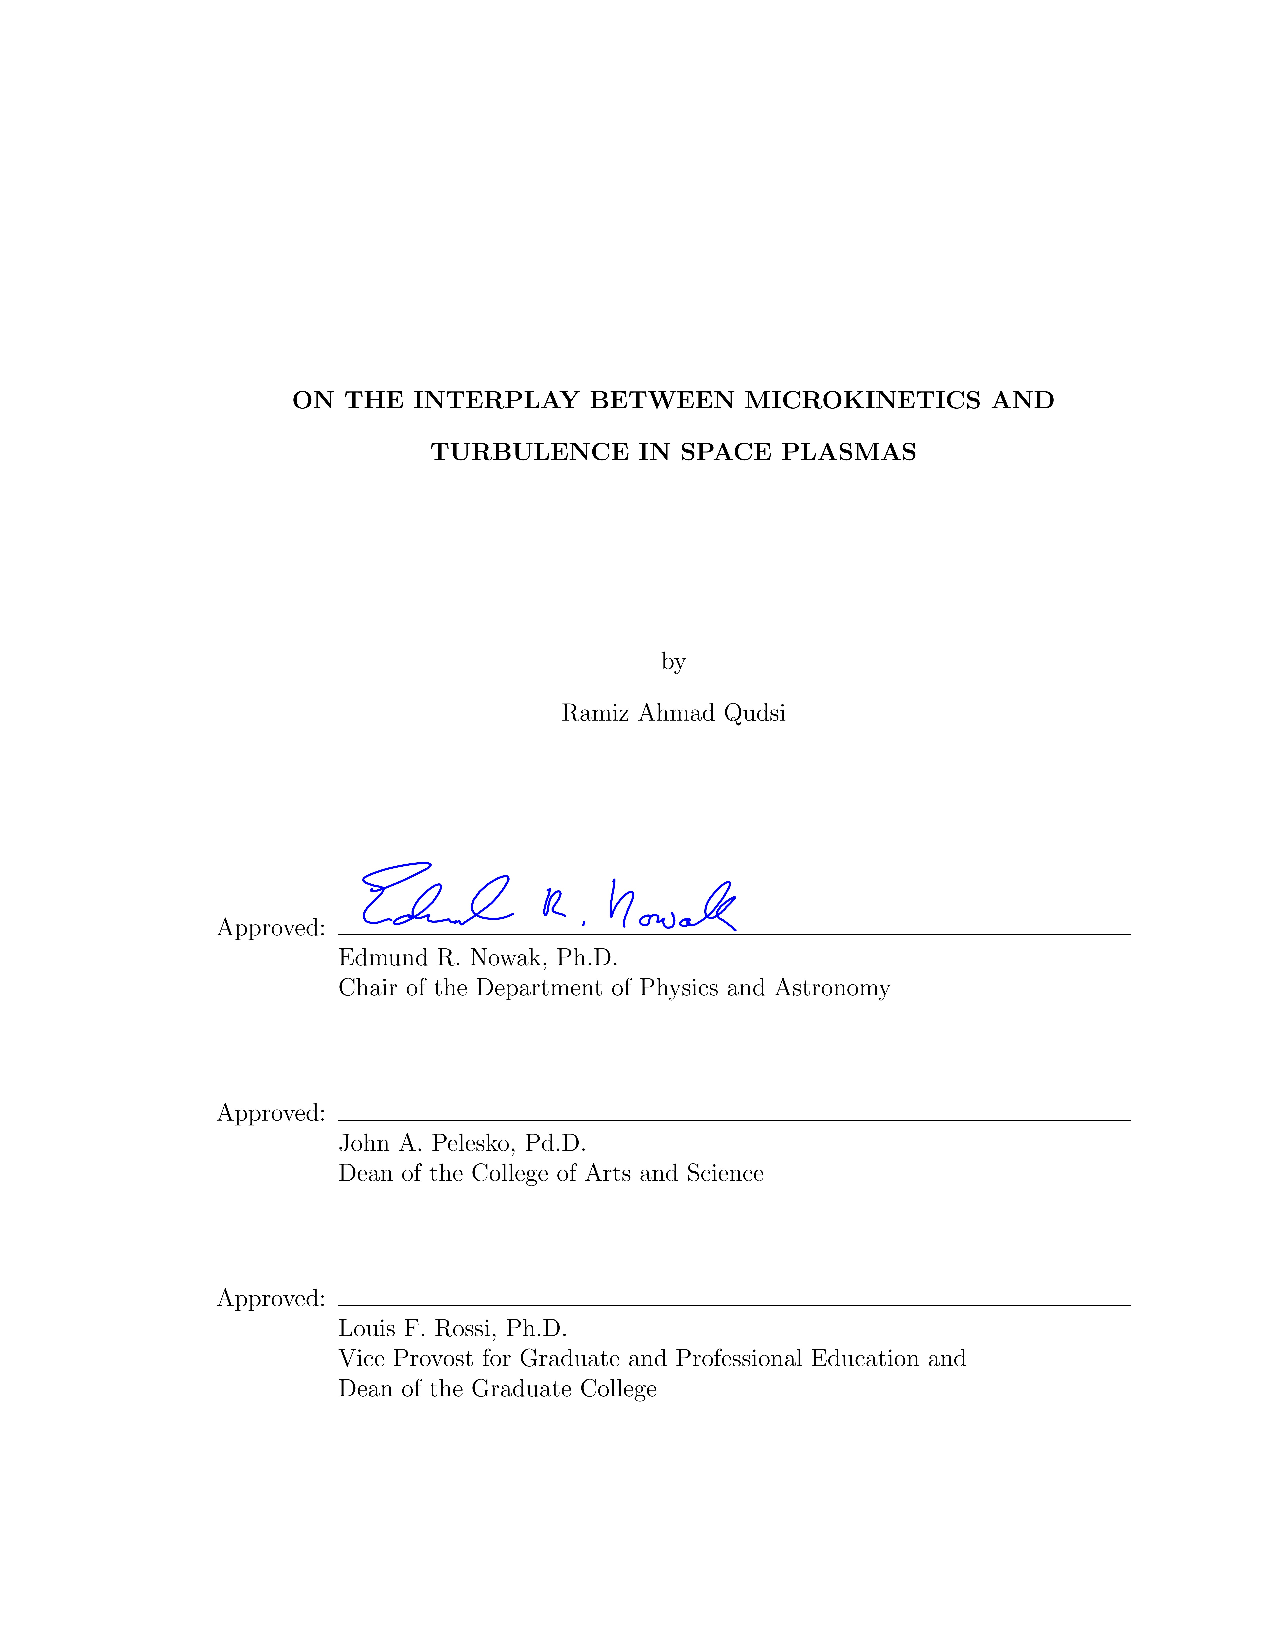
\includepdf{figures/signatures/dissertation-main_signature_pages_p2.pdf}
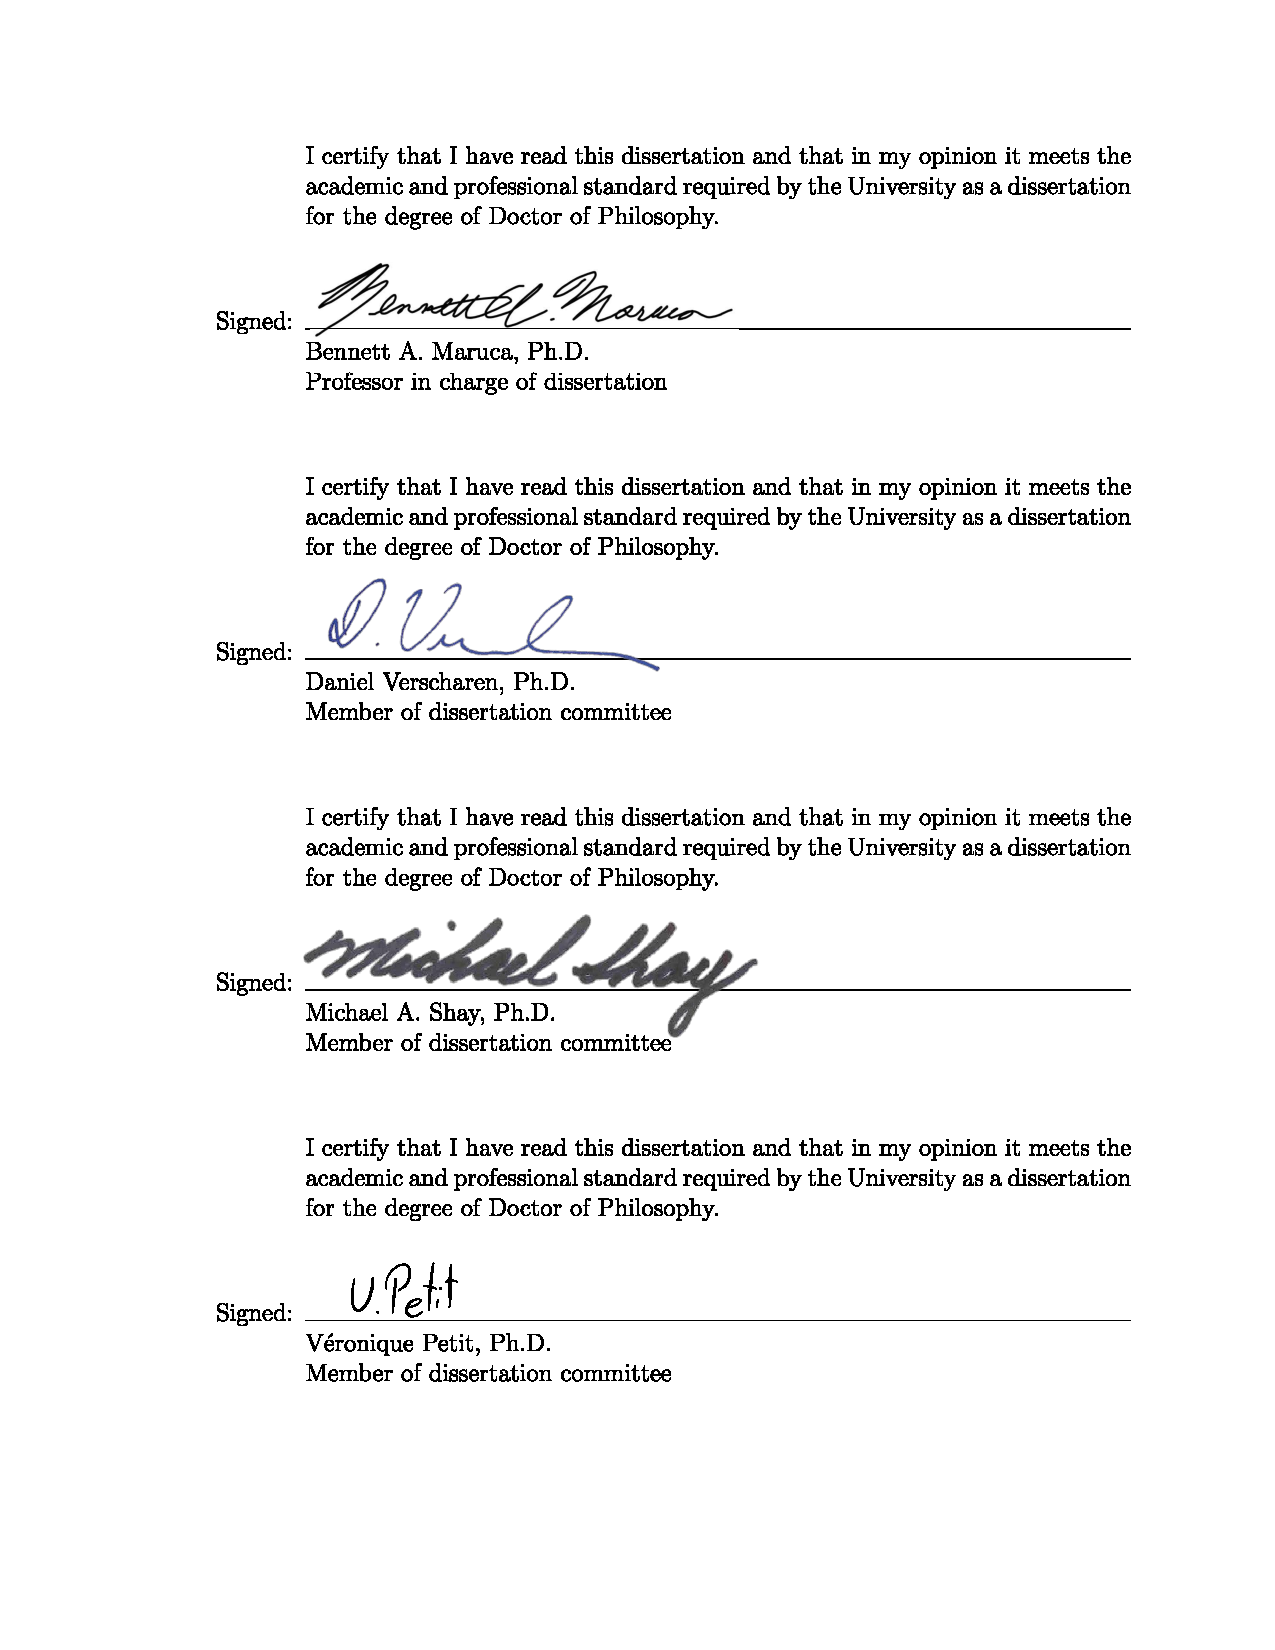
\includepdf{figures/signatures/dissertation-main_signature_pages_p3_v2.pdf}

\includepdf{figures/signatures/dissertation-main_signature_pages_p4-whm.pdf}

\begin{front} % Starts front material (Roman style page numbers)

\newpage\null\thispagestyle{empty}\newpage

\prefacesection{ACKNOWLEDGEMENTS}
%
% This is the acknowledgement file (acknowl.tex)
%
%\Acknowledgement
%\begin{center}
%    \vspace{3em}
%    \LARGE{ACKNOWLEDGEMENTS}   
%\end{center}

I would like to thank my thesis supervisor, Dr.~Bennett Maruca, for his constant support and
understanding during the whole duration of my graduate education. He has been a source of
inspiration and encouragement.

I would like to thank my colleagues in the department with whom I have had innumerable discussions
on all topics, academic and otherwise. A lot of ideas presented in this thesis originated during one
of those discussions. Coffee-shop meetings with Dr.~Bill Matthaeus was THE place for such
discussion. I am especially indebted to Tulasi Parashar and Rohit Chhiber, who were always very
patient while explaining nuances of plasma physics to me. Alexandros Chasapis was always encouraging
and informative as we discussed the subtleties of multi-spacecraft techniques. Discussion with
Riddhi, Mark, Debanjan, and Manuel were always animated, fun, educational and diverse. I am
specially indebted to Bill and Riddhi who always took time to explain finer points of turbulence. I
am so glad to have been part of such a dynamic and diverse group.

I feel lucky to have had the chance to work with Dr.~Peter Gary who was always excited about the
kind of work we were doing. His comments on our results were always insightful and encouraging and
his enthusiasm for discussion was contagious. He will be fondly remembered and dearly missed!

I am very thankful to the MMS and PSP teams for giving me the opportunity and most importantly data
to work with.

Life in Newark was filled with fun and I depart here with lots and lots of memories. Thanks to all
my friends who contributed to the joy of living there. Siddhi, Sucharita, Mehul, Abdul, Sameer,
Mark, Khushboo, Aditya, Abhishek, Prasanna, Anitha, Vrathasha; thank you all for making my stay so
much enjoyable.

Special thanks to Krishna who has been supportive and understanding throughout thesis writing
process and helped in typing a not so insignificant part of this thesis.

I would also like to thank the staff of the Department of Physics and Astronomy, especially Maura,
Elle, Angie and Linda, who have been extremely helpful over the years and very proactive in solving
my non-academic issues. Sansern Somboonsong and Zelphia Johnson were always very responsive to my
queries regarding the computer and network.

I would like to thank my family, who despite their own biases against science, have largely been
supportive my own endeavors in the field.

And lastly I would like to thank my dear friend Abhishek Maniyar. I decided to leave my job, and a
good job it was, because he insisted that I should and pursue my dream of a PhD in Physics. He
guided me through the whole process and I am extremely thankful to him for making me do that. Thank
you Maniyar for being the force behind this!

This research made use of PlasmaPy, a community-developed open source Python package for plasma
science \citep{misc:Plasmapy2020}. I extensively used the SAO/NASA
\href{https://ui.adsabs.harvard.edu/}{Astrophysics Data System (ADS)} in the preparation of this
dissertation. % This file (acknowl.tex) contains the text
                % for the acknowledgments or type text here.

% Table of Contents is always created, but you may set \tablespagefalse and \figurespagefalse if you
% don't want these generated automatically (i.e. List of Tables and List of Figures).  These are set
% to true by default (i.e. \tablespagetrue, \figurespagetrue).

% Uncomment if you do not want a List of Figures.  \figurespagefalse

% Uncomment if you do not want a List of Tables.  \tablespagefalse 

%\tableofcontents
\maketocloflot
%\newpage\null\thispagestyle{empty}\newpage

\prefacesectiontoc{Abstract}
%
% This is the abstract A file (abstract.tex)
%
%\Abstract{Title of Abstract}
Space plasmas in the inner heliosphere exist in a weakly collisional and turbulent state. Though
energy transfer from large scales to smaller scales by turbulent cascade is widely accepted as an
important feature of space plasmas, details of its exact dissipation process are lacking. Features
arising because of turbulence, such as intermittency and temperature anisotropy, play important
roles in the dynamics of space plasmas. Microkinetic linear instabilities induced by temperature
anisotropy have been shown to change the statistical characteristics of plasma in a significant way.

Since the two processes, turbulence cascade and microkinetic instabilities, occur in the same
physical and phase space, there is an interplay at work. In this study we investigated this
interplay and the subsequent competition arising between the two, linear and nonlinear, processes.
We found an explicit connection between intermittency and linear instability growth rates. We also
showed localization of temperature enhancement regions along the intermittent structures, which in
turn can trigger linear instabilities. Investigation of the two processes shed light on why linear
theory works as well as it does, and shows the complicated nature of their interplay.

Information related to the exact spatial structure of the interplanetary magnetic field is vital to
our understanding of the type of turbulence active in the space plasmas and the mechanism of
turbulence cascade. This will help us discern the interplay between the two processes. We thus also
report on a proof of concept study of magnetic field topology reconstruction using Gaussian
Processes in machine learning. % This file (abstract.tex) contains the text
                 % for an abstract or type text here.

%
% This is the epigraph file (epigraph.tex)
%
%\newpage\null\thispagestyle{empty}
%\begin{center}
%    \begin{figure*}
%        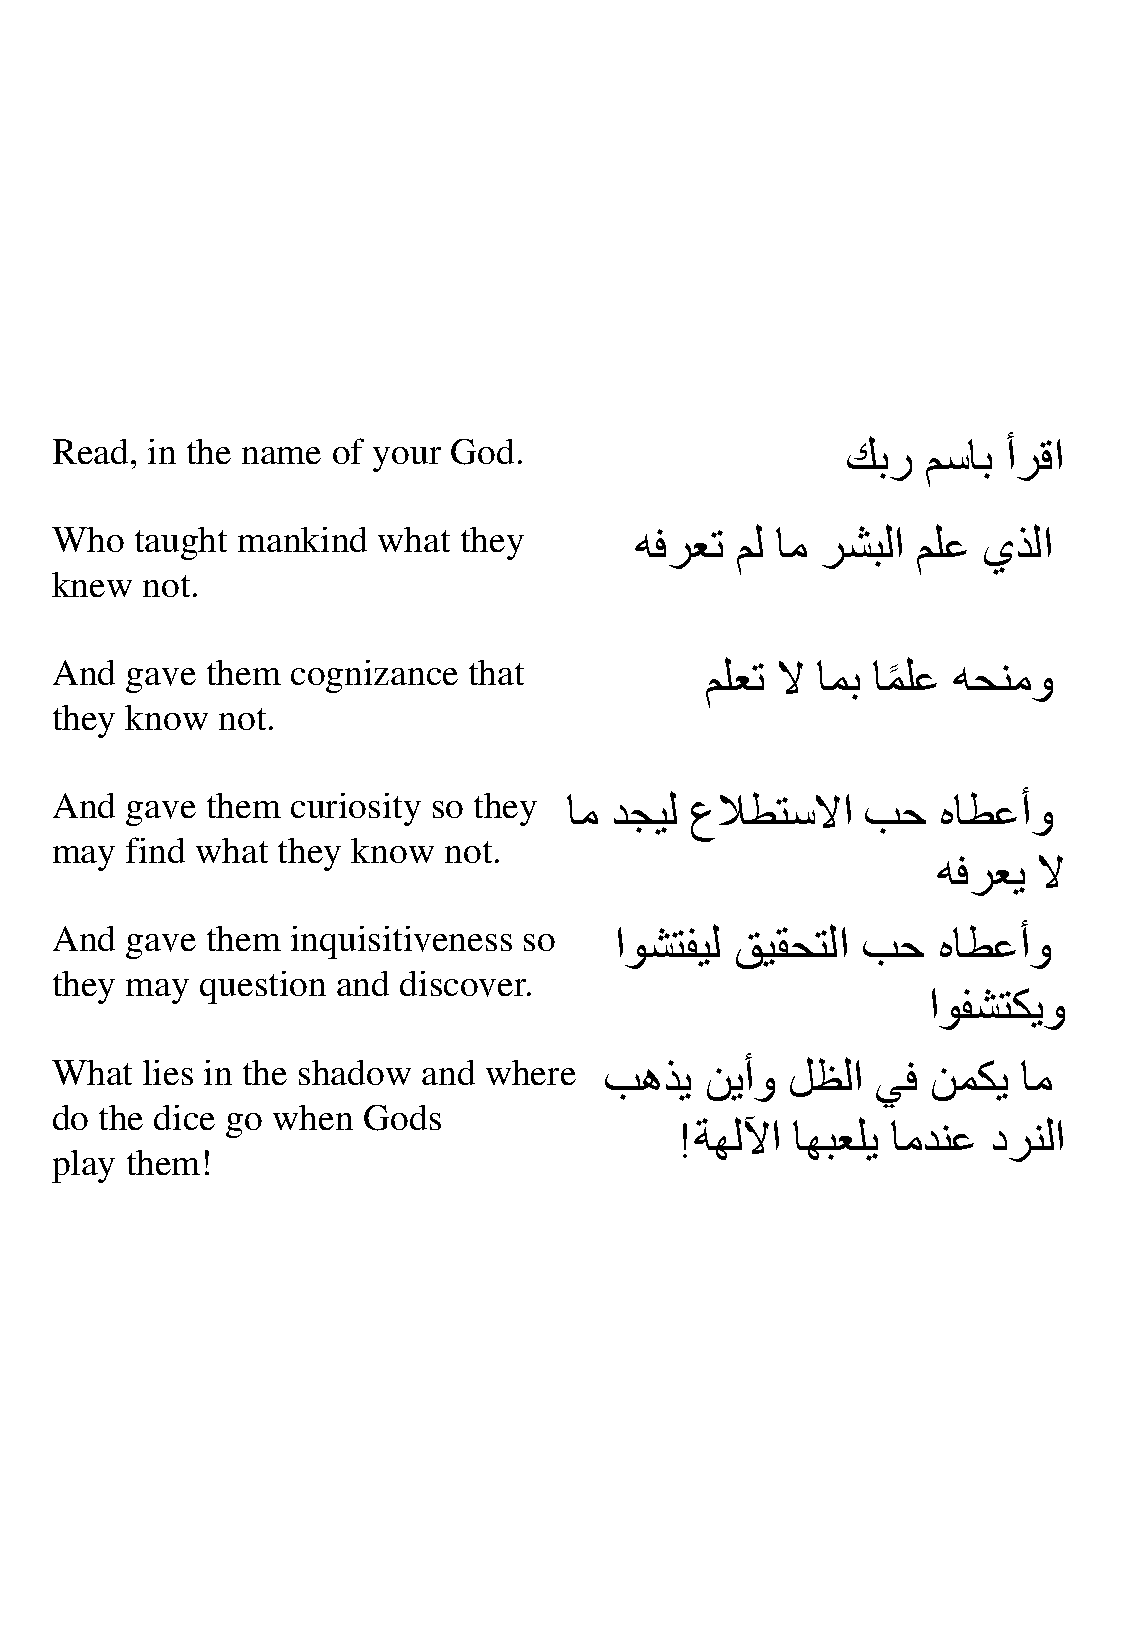
\includegraphics[width=1\textwidth]{figures/epigraph/thesis_epigraph_v2.pdf}
%        \captionsetup{labelformat=empty}
%        \caption[]{}
%    \end{figure*}
%\end{center}

\newpage\null\thispagestyle{empty}\newpage
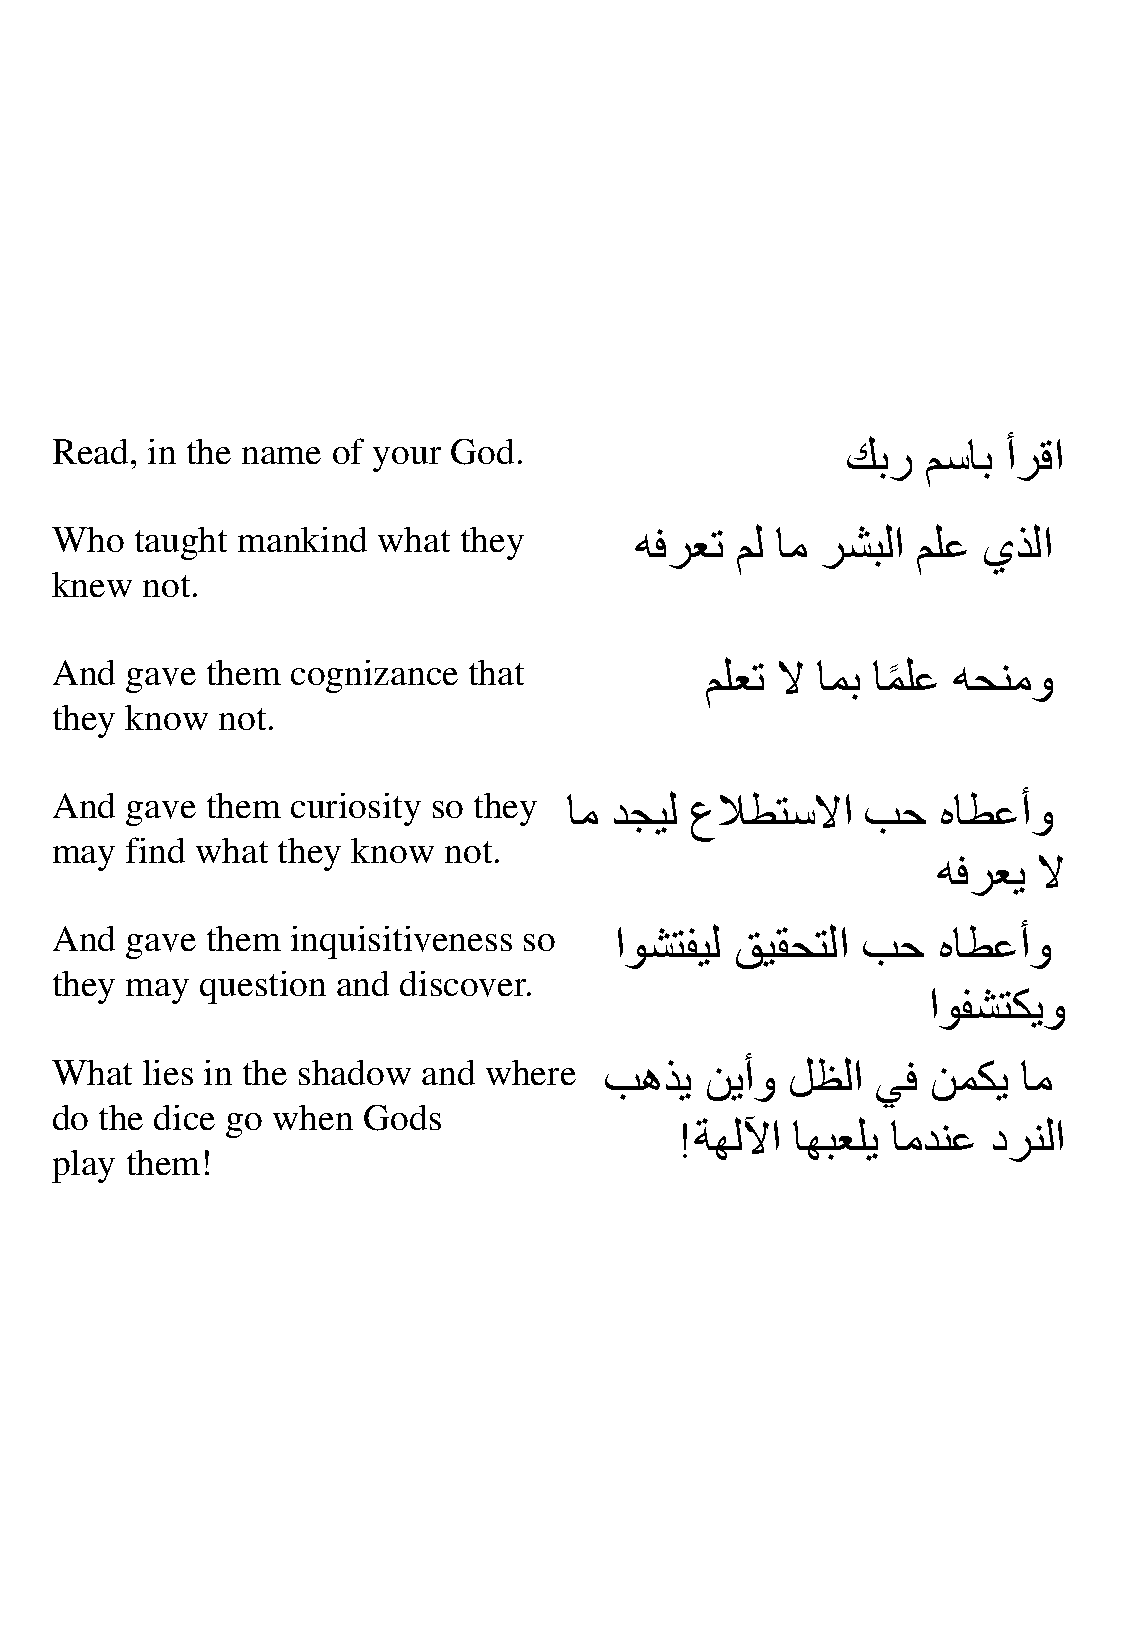
\includepdf{figures/epigraph/thesis_epigraph_v2.pdf}

\newpage\null\thispagestyle{empty}\newpage

\vspace*{\fill} \hspace{-3.2em}“This is a work of fiction. Still, given an infinite number of possible
worlds, it must be true on one of them. And if a story set in an infinite number of possible worlds
is true in one of them, then it must be true in all of them. So maybe, it's not as fictional as we
think.”\\
\hspace*{0pt}\hfill ― Neil Gaiman, InterWorld
\vspace*{\fill}

\newpage\null\thispagestyle{empty}\newpage % This file (epigraph.tex) contains the text
                 % for the epigraph

\end{front}
                   % This file (dissertation-tap.tex) contains the Title
                   % and Approval Page information for a dissertation.

%\newpage\null\thispagestyle{empty}\newpage

%\include{cistercian_numerals}

%%
% This is the epigraph file (epigraph.tex)
%
%\newpage\null\thispagestyle{empty}
%\begin{center}
%    \begin{figure*}
%        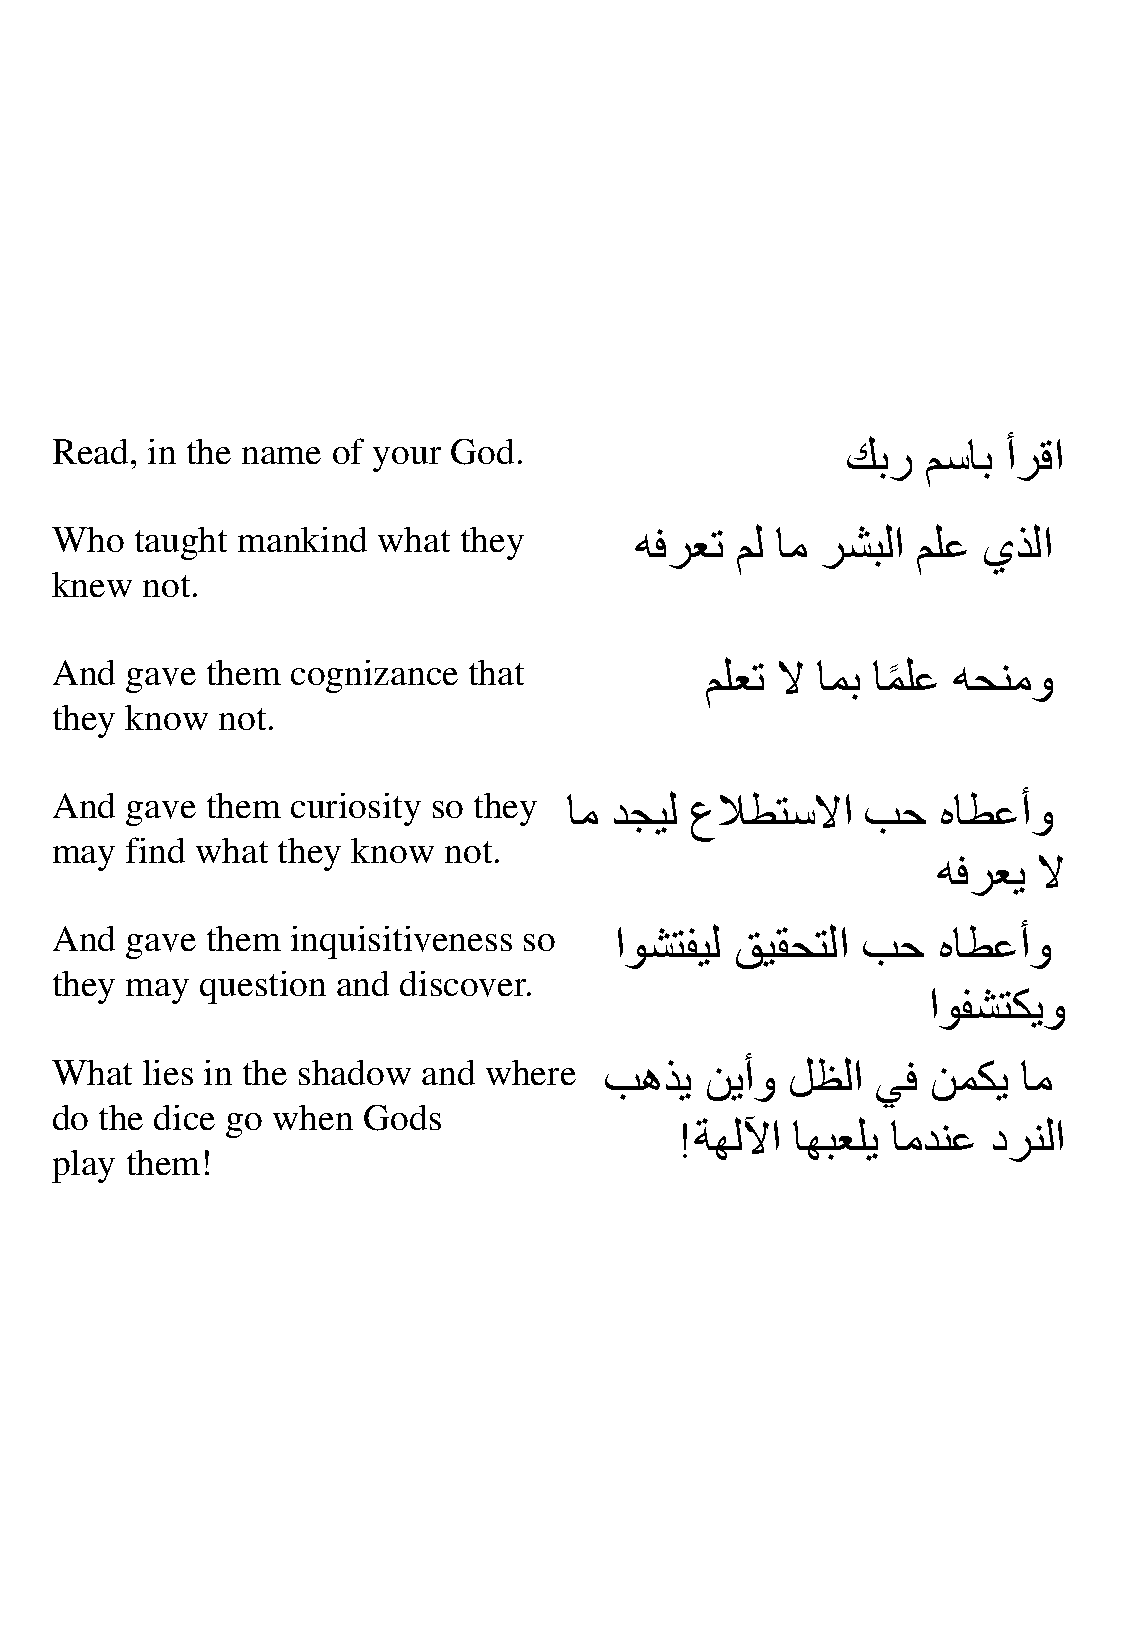
\includegraphics[width=1\textwidth]{figures/epigraph/thesis_epigraph_v2.pdf}
%        \captionsetup{labelformat=empty}
%        \caption[]{}
%    \end{figure*}
%\end{center}

\newpage\null\thispagestyle{empty}\newpage
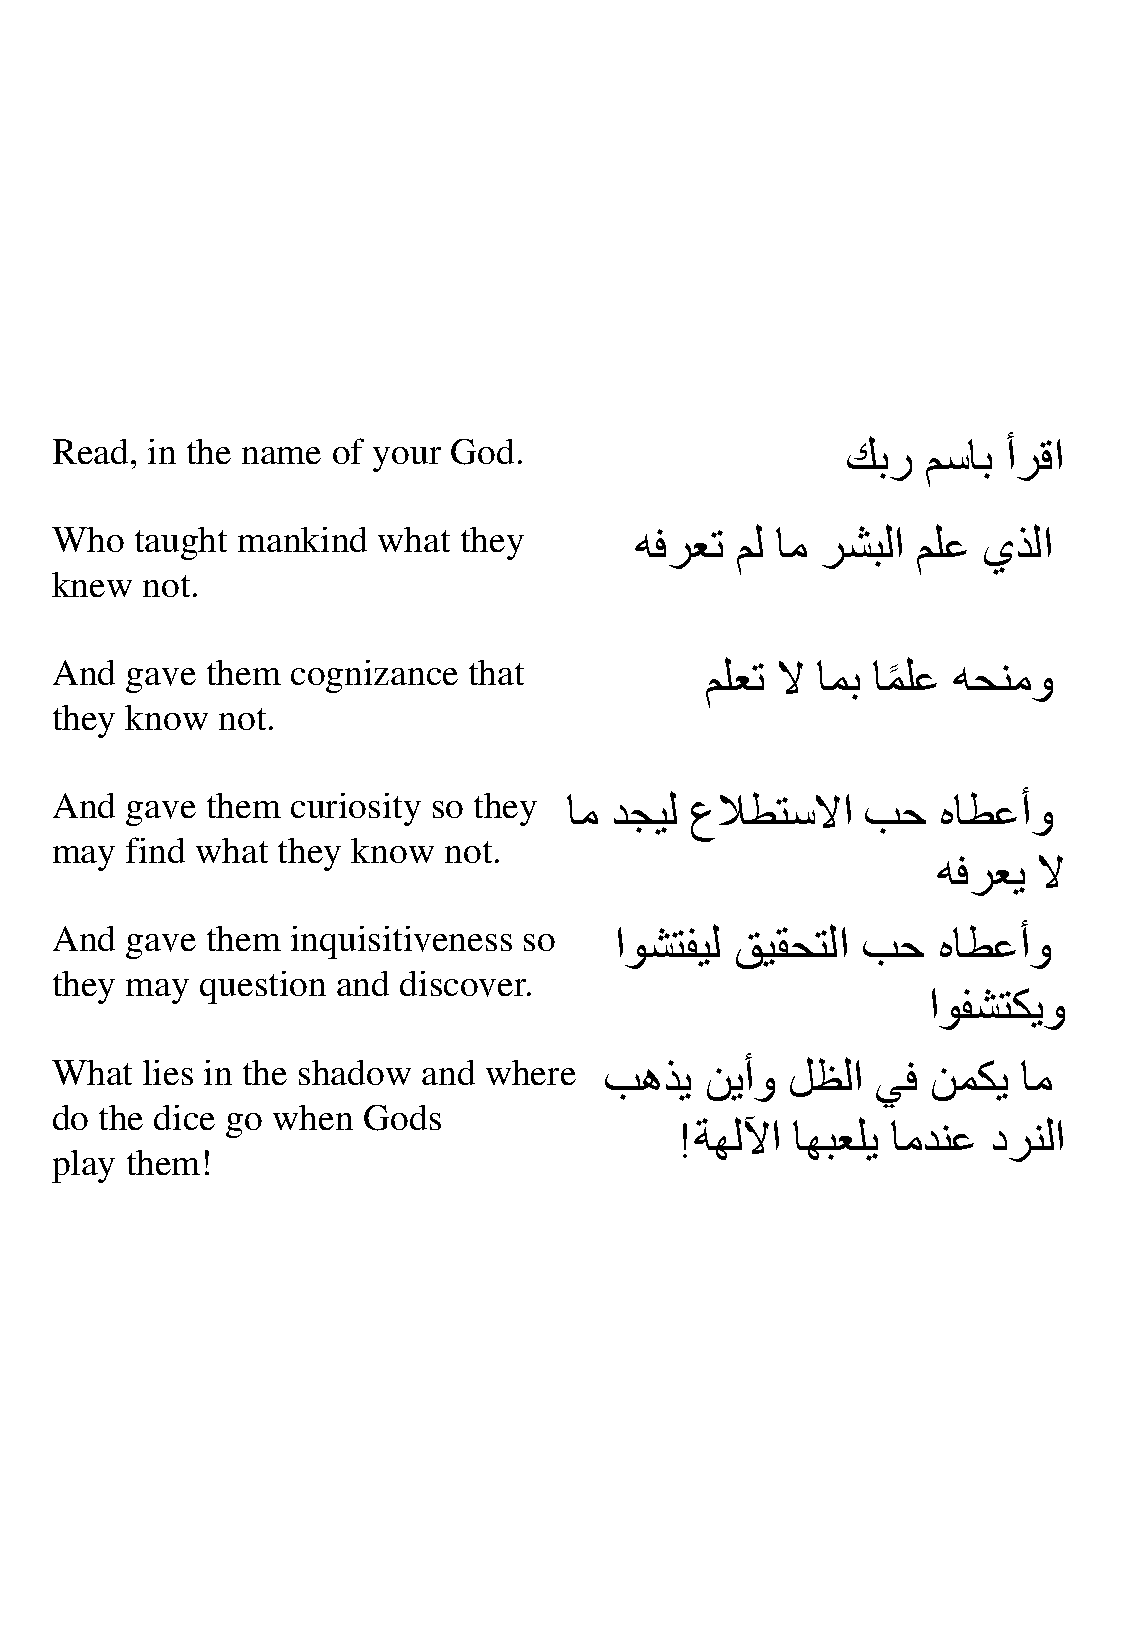
\includepdf{figures/epigraph/thesis_epigraph_v2.pdf}

\newpage\null\thispagestyle{empty}\newpage

\vspace*{\fill} \hspace{-3.2em}“This is a work of fiction. Still, given an infinite number of possible
worlds, it must be true on one of them. And if a story set in an infinite number of possible worlds
is true in one of them, then it must be true in all of them. So maybe, it's not as fictional as we
think.”\\
\hspace*{0pt}\hfill ― Neil Gaiman, InterWorld
\vspace*{\fill}

\newpage\null\thispagestyle{empty}\newpage % This file (epigraph.tex) contains the text
                   % for epigraph.

%
% This is Chapter 1 file (chap1.tex)
%
\chapter{Introduction}\label{chap:chap1}

    \section{Prologue to Plasma}\label{sec:plas0}

        Our daily life is dominated by our interactions with the three classical states of matter:
        solid, liquid and gas. Plasma is the fourth state of matter and by far the most abundant
        one. In fact the observable universe is almost entirely made up of plasma (99.9\% of the
        universe) \citep{Boulos1994}. From the HII region around a huge star to the surface of a
        star, from the super hot Inter Galactic Medium to the inside of a plasma TV, plasma is
        everywhere. Given its abundance and ubiquitous nature, it becomes vitally important to study
        and understand plasma. In the rest of this chapter we define what constitutes a plasma
        (\Cref{sec:plas1}) and  discuss some of its salient properties and the laws of physics that
        govern it. We also shed some light on the local regions around Earth that are made up of
        plasma (\Cref{sec:plas2}) and discuss studying them (\Cref{sec:plas3}). We conclude the
        chapter with with a brief discussion of topics covered in this thesis. (\Cref{sec:plas4}).

    \section{Introduction To Plasma} \label{sec:plas1}

        The term ``plasma" comes from the ancient Greek word ``$\pi \lambda \acute{\alpha} \sigma
        \mu \alpha$" that means something that is moldable. It was first used in the modern context
        by \citet{Langmuir1928} to describe the ``region (around electrodes) containing balanced
        charges of ion and electrons".
        
        A plasma is a sub-type of ionized gas; a gas where significant fraction of the atoms have
        been ionized. There are specific criteria that distinguishes plasmas from other ionized
        gases (discussed later in this section), but first we consider the equations that govern the
        dynamics of charged particles (electrons and ions).

        As is with everything that has mass in the universe, a plasma's dynamics is governed by
        Newton's equation of motion:
        \begin{align}
            %\begin{split}
            \mathbf{F}_{\rm net} = \frac{d \mathbf{P}}{d t} & = m \frac{d^2 \mathbf{x}}{d t^2} \protect\footnotemark \label{eq:nwtn1}
        \end{align}
        \footnotetext{$\mathbf{F}_{\rm net} = m \frac{d^2 \mathbf{x}}{d t^2}$ is only valid when the
        particle is moving at speed much smaller than the speed of light.} where $\mathbf{F}_{\rm
        net}$ is the net external force acting on the system and \textbf{P} is its momentum. t is
        time, \textbf{x} is the position vector and $\frac{d}{dt}$ is the derivative with respect to
        time.
        
        For a charged particle with charge \textit{q}, moving with velocity \textbf{v} in an
        electromagnetic field with electric and magnetic field as \textbf{E} and \textbf{B}
        respectively, the electromagnetic force or Lorentz force is given as:
        \begin{align}
            \mathbf{F}_{\rm EM} = q \left( \mathbf{E} + \mathbf{v} \times \mathbf{B} \right)
            \label{eq:lorentz}
        \end{align}
        These equations (\Crefrange{eq:nwtn1}{eq:lorentz}) coupled with the four Maxwell's equations
        (\Crefrange{eq:maxwell1}{eq:maxwell4}) define the complete dynamics of a plasma.
        \begin{align}
            \nabla \cdot \mathbf{E} & = \frac{\rho}{\epsilon_\circ} \label{eq:maxwell1}\\
            \nabla \cdot \mathbf{B} & = 0 \label{eq:maxwell2}\\
            \nabla \times \mathbf{E} & = -\frac{\partial \mathbf{B}}{\partial t} \label{eq:maxwell3}\\
            \nabla \times \mathbf{B} & = \mu_\circ \mathbf{J} + \frac{1}{c^2} \frac{\partial \mathbf{E}}{\partial t} \label{eq:maxwell4}
            %\end{split}
        \end{align}
        where, $\rho$ is the charge density, $\epsilon_\circ$ is the permittivity of free space,
        $\frac{\partial}{\partial t}$ is the partial derivative with respect to time, $\mathbf{J}$
        is the current density, and c is the speed of light in vacuum.

        The most accurate way to study the behaviour of plasma is to track each particle
        individually using \Crefrange{eq:nwtn1}{eq:maxwell4}, all while accounting for all the
        fields, external as well as those arising because of the charge and motion of particles
        themselves. However, that method is almost impossible to implement not only because of
        difficulty in computing the field arising because of mutual interactions but also because of
        the huge number of particles involved. Consequently, scientists often fall back to
        statistical methods in their studies, such as applying kinetic equations that use physics
        based on ensemble averages (see \Cref{chap:chap2}) or by approximating the plasma as a fluid
        as is done in Magneto-hydrodynamics (MHD).

        Since even the lightest ion, a proton, is nearly 2000 times more massive than an electron
        and the dynamics of particles are often governed by their masses, both the time and length
        scales at which dynamics occur in plasmas are extremely diverse, even when one is studying
        the same phenomena for ions and electrons. Values of some of the parameters associated with
        plasma (generally referred to as \textit{plasma parameters}) can help in understanding the
        scales one is dealing with. Also, as will become apparent in \Cref{chap:chap2,chap:chap3},
        one may choose to focus on a specific scale depending on the interest or scope of the study.
        Here, we list some of the most relevant plasma parameters, what each one of them mean, and
        their mathematical expressions.\\
        \\
        \textbf{Debye Length} ($\lambda_{\rm D}$): The Debye length \index{Debye length} is the scale above which a
        plasma (with no net charge) maintains near charge neutrality --- $\rho \approx 0$ when
        $\rho$ is smoothed over a scale $\gtrsim \lambda_{\rm D}$. On scales smaller than
        $\lambda_{\rm D}$, particles behave as if it were interacting with other moving charges
        individually instead of a smooth macroscopic electromagnetic field. If we have sufficiently
        large number of particles inside a spherical volume with $\lambda_{\rm D}$ as the radius
        ($n_{\rm p} \lambda_{\rm D}^3 > 1$), then particles are shielded by its neighbours from the
        surrounding plasma (called \textit{Debye shielding}). On scales $\lesssim \lambda_{\rm D}$,
        random thermal motions of the particles give rise to isolated regions of non-zero charge
        density.  We would then expect $\lambda_{\rm D}$ to increase with plasma temperature.
        Indeed, for a plasma consisting of ionized hydrogen for which the protons and electrons have
        comparable temperatures, we define Debye length as:
        \begin{align}
            \lambda_{\rm D} & = \frac{\epsilon_\circ k_{\rm B} T_{\rm p}}{n_{\rm e} e^2}^{1/2} \label{eq:debye}
        \end{align}
        where $k_{\rm B}$ is the Boltzmann constant, $n_{\rm e}$ is the electron number density and
        $T_{\rm p}$ is the proton temperature. In order for a system to be classified as plasma, we
        must have the physical length scale (L) of the system much larger than its Debye length.
        \begin{align}
            \lambda_{\rm D} \ll L \label{eq:lambda}
        \end{align}
        \\
        \textbf{Ion-inertial Length \index{Ion-inertial Length}($d_{\rm j}$):} This is the length scale in plasma at which the
        electrons are decoupled from ions and the magnetic field is frozen in with the electrons.
        For species `$j$' of plasma (where $j = p^{+}$ for protons and $j = i^{n+}$ for any other
        ion with n positive charge)\footnote{In this thesis unless otherwise specified ion will
        refer to protons and two terms will be used interchangeably}, it can be written in terms of
        ion plasma frequency ($\omega_{\rm pj}$) as:
        \begin{align}
            d_{\rm j} = \frac{c}{\omega_{\rm pj}} \label{eq:ionint}
        \end{align}
        \\
        \textbf{Plasma Frequency \index{Frequency!plasma} ($\omega_{\rm pj}$)}\footnote{Note that `p' in $\omega_{\rm pj}$
        refers to plasma and not proton.}: It is the frequency at which any given species in plasma
        oscillates and is given by:
        \begin{align}
            \omega_{\rm pj} & = \left(\frac{n_{\rm j} q_{\rm j}^2}{\epsilon_\circ m_{\rm j}}\right)^{\frac{1}{2}} \label{eq:plasf}
        \end{align}
        \\
        \textbf{Cyclotron Frequency \index{Frequency!cyclotron} ($\Omega_{\rm cj}$):} In a magnetized plasma (a plasma which has
        a background magnetic field), due to the perpendicular direction of the magnetic force with
        respect to the particle's velocity, any non-stationary charged particle in a magnetic field
        gyrates around a point called the center of gyration. The frequency of gyration or cyclotron
        frequency is given by:
        \begin{align}
            \Omega_{\rm cj} & = \frac{q_{\rm j} B}{m_{\rm j}} \label{eq:cyclf}
        \end{align}
        where \textbf{B} is the background magnetic field. \\
        \\
        \textbf{Gyroradius \index{Gyroradius}}\textbf{($\rho_{\rm j}$)}: This is the radius of the circular path that a particle takes in
        the presence of a magnetic field, and is dependent on the ratio of thermal speed to that of
        cyclotron frequency.
        \begin{align}
            \rho_{\rm j} = \frac{w_{\rm j}}{\Omega_{\rm cj}} \label{eq:rho}
        \end{align}
        where $w_{\rm j}$ is the thermal speed of the particle. \\
        \\
        \textbf{Alfv\'en Speed \index{Alfv\'en Speed} ($V_{\rm Aj}$)}: It is the speed at which magnetic signals, like a
        fluctuation in the field, travel in a plasma. It depends on the strength of the magnetic
        field in the plasma as well the density and mass of the species and has the following
        expression:
        \begin{align}
            v_{\rm Aj} = \frac{B}{\sqrt{\mu_\circ \sum_{\rm j} n_{\rm j} m_{\rm j}}} \label{eq:alfv}
        \end{align}

    \section{Plasma in Near-Earth Environment} \label{sec:plas2}

        The Sun is the largest source of plasma in our solar system. Huge amounts of charged
        particles emanate from the Sun originating in its outermost atmospheric layer, called the
        Corona \citep{Parker1958,Parker1960,Parker1963,Gringauz1960,Neugebauer1962}. This constant
        outflow of particles is commonly called solar wind. The solar wind is often highly
        magnetized, is weakly collisional, travels at supersonic speed and is primarily composed of
        ionized hydrogen (i.e., protons) \citep{Marsch1982}. \Cref{tab:plaspar1} lists out some of
        the plasma parameters and their typical values for the solar wind at 1\,au.
        \Cref{fig:plas_para_wnd} shows the distribution of some of the parameters listed in
        \Cref{tab:plaspar1}.
        \begin{figure}
            \begin{center}
                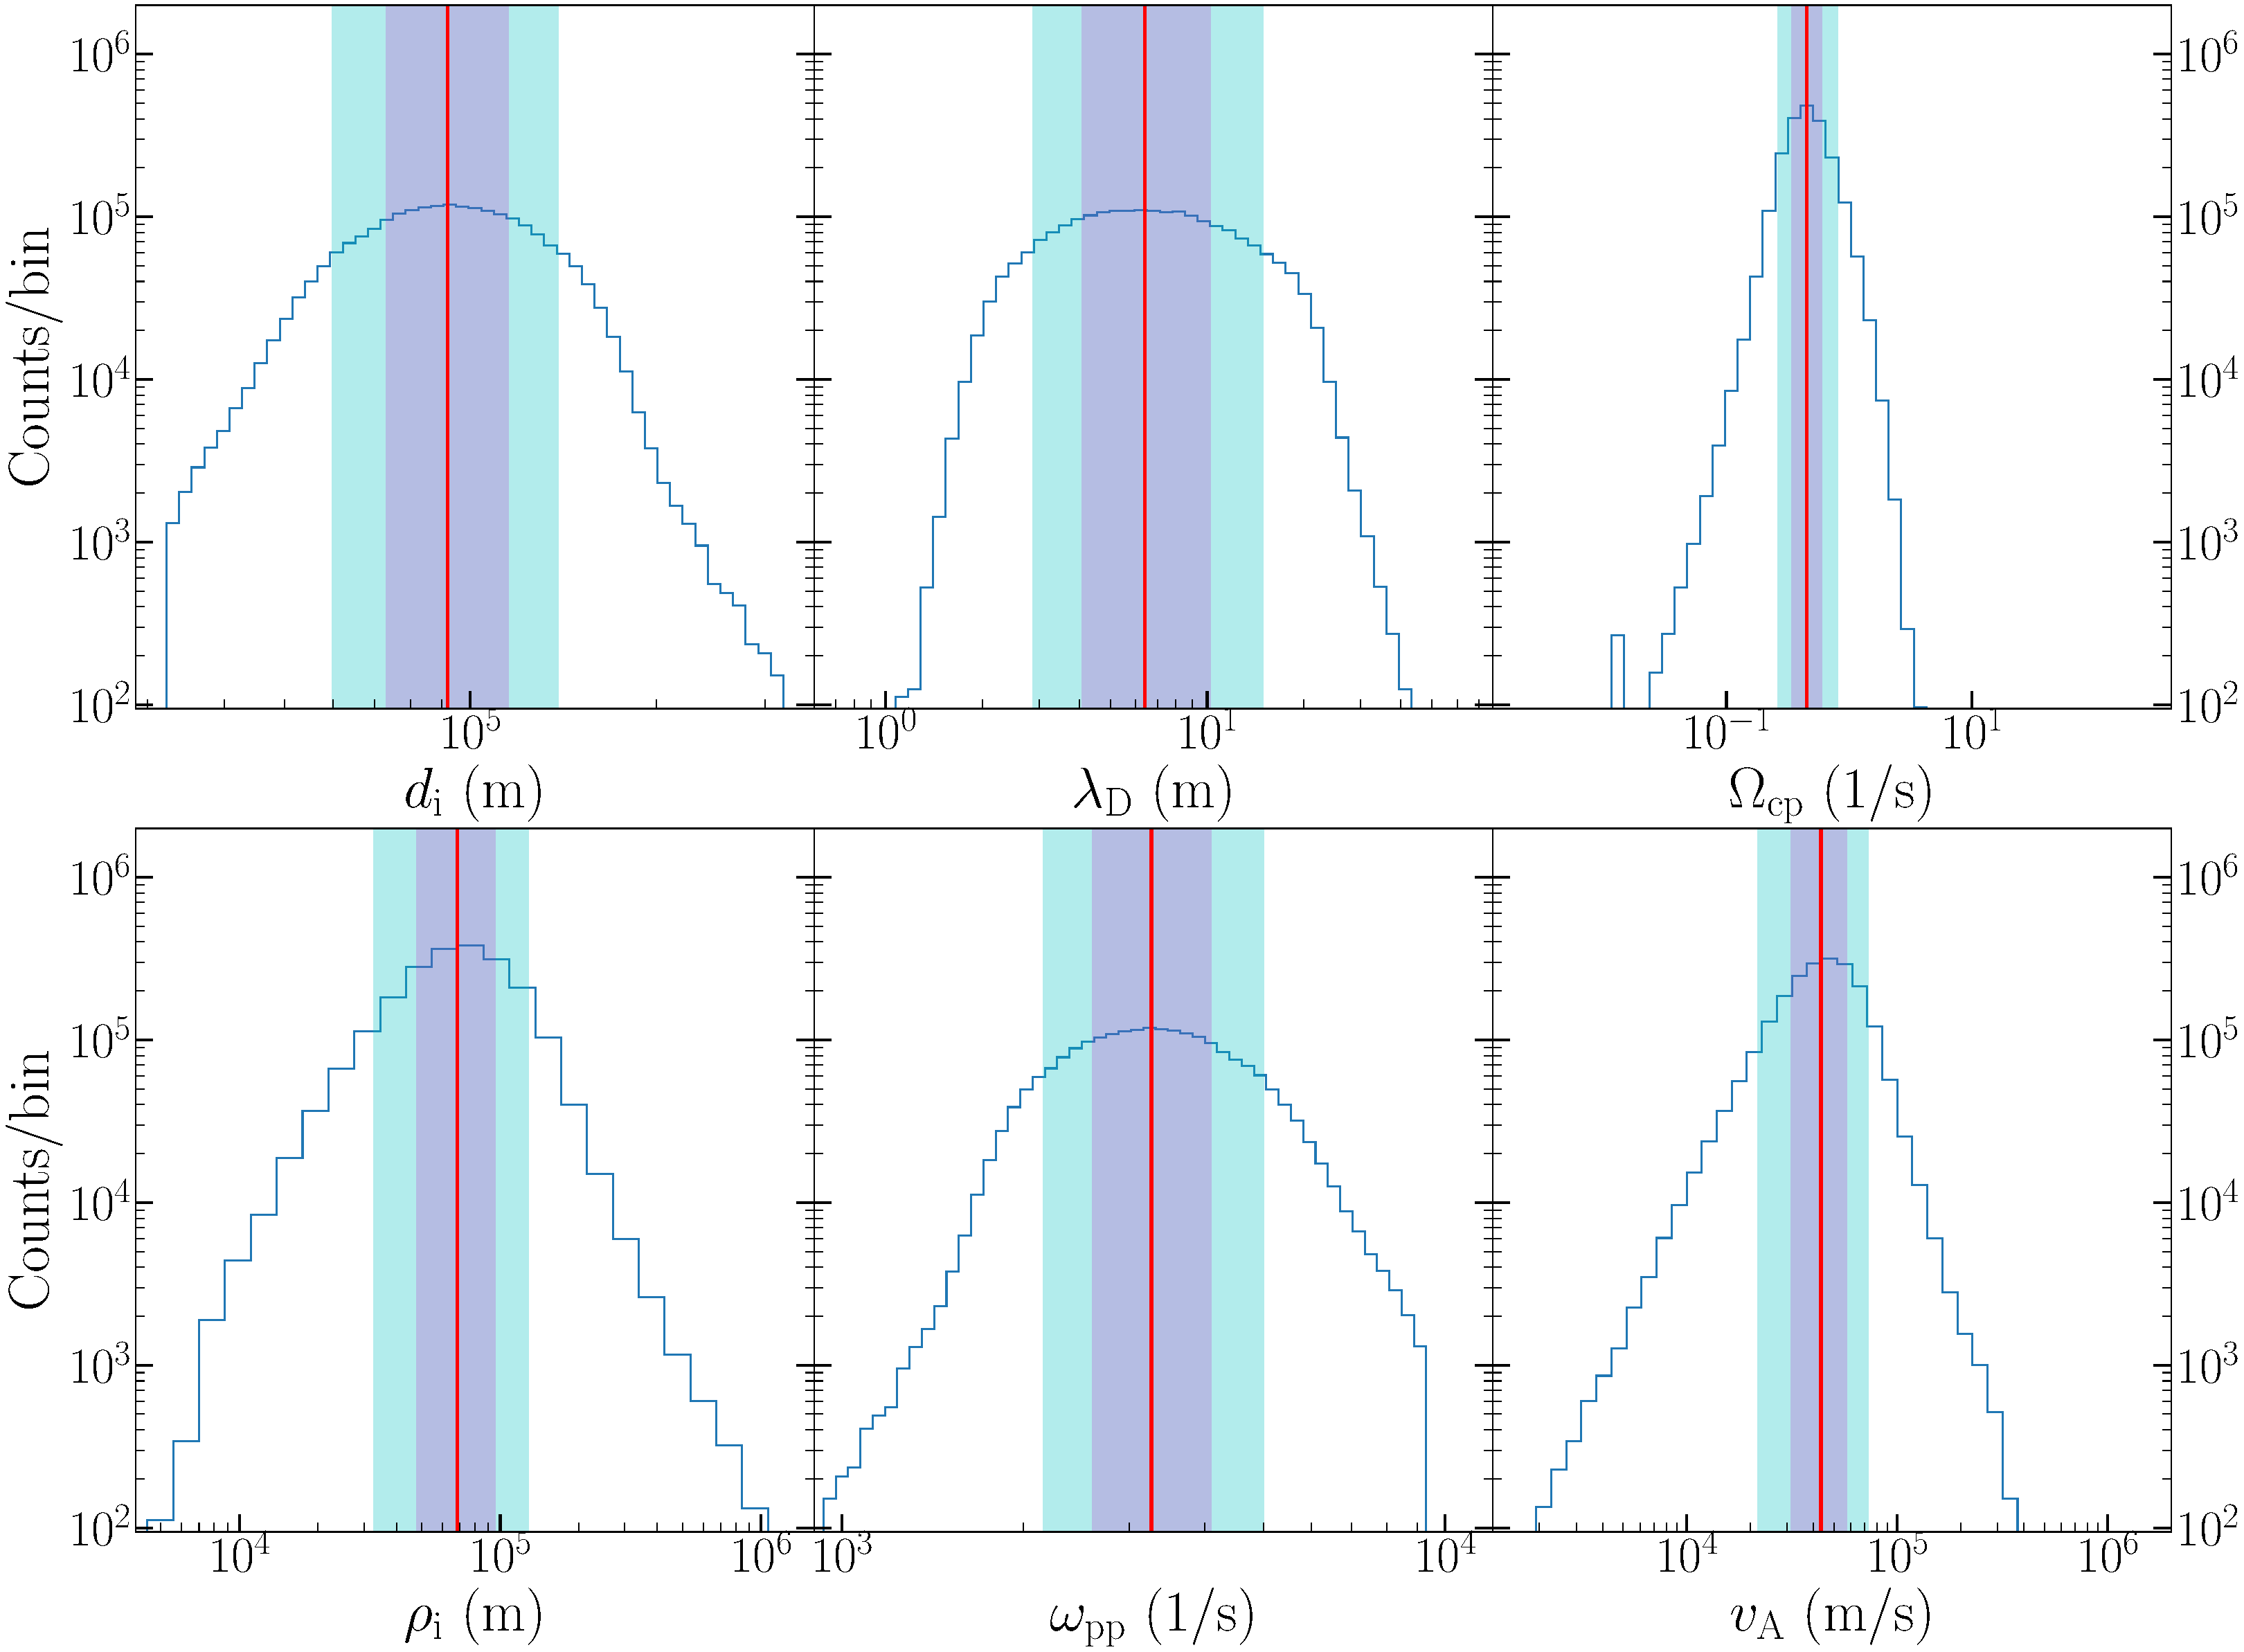
\includegraphics[width=1\textwidth]{figures/chap1/plasma_parameters_wnd.pdf}
                \caption[Plasma parameter distributions at 1\,au ]{Distribution of various plasma
                parameters near Earth, based on data from Wind spacecraft. Top row shows
                distribution for (from left to right) proton-inertial length ($d_{\rm i}$), Debye
                length ($\lambda_{\rm D}$), proton-gyrofrequency ($\Omega_{\rm cp}$) and the lower
                row shows (from left to right) proton-gyroradius ($\rho_{\rm i}$), proton-plasma
                frequency ($\omega_{\rm pp}$) and alfv\'en speed ($v_{\rm A}$). Red line shows the
                median value of each parameter, whereas the shaded region shows $10^{\rm th}$ to
                $90^{\rm th}$ (cyan) and $25^{\rm th}$ to $75^{\rm th}$ percentile (magenta) of each
                parameter.\protect\footnotemark}
                \label{fig:plas_para_wnd}
            \end{center}
        \end{figure}
        \footnotetext{\Cref{fig:plas_para_wnd} is based on data from Wind Spacecraft. See
        \Cref{sec:wind} for more details on data and spacecraft.}

        The Earth's local magnetic field, which arises as a result of dynamo action of its molten
        core \citep{Elsasser1956}, extends far into space (roughly 10 earth radii in the direction
        of the sun and $\sim$ 300 earth radii in the anti-sunward direction) and interacts with the
        incoming solar wind. This interaction gives rise to a plethora of structures.
        \Cref{fig:ms_earth} shows an artistic rendition of Earth's magnetosphere. The layer along
        which solar wind transitions from supersonic to subsonic speed is called the bow shock
        (region 1). The region immediately after the bow shock is called the magnetosheath (region
        2) and is comprised mostly of shock treated solar wind. This region is of special importance
        to the present work (see \Cref{chap:chap5,chap:chap7}). The region beyond the magnetosheath,
        towards Earth, where the pressure exerted by the solar wind and Earth's magnetic field are
        in equilibrium is called the magnetopause (region 3) and forms the boundary between Earth's
        magnetosphere (volume  around  Earth  where the influence  of  its magnetic field is felt
        (region 4)) and the solar wind. There is also a long magnetotail further away from the Sun,
        which extends far beyond the surface of the Earth (regions 5 and 6). The region closest to
        the surface (region 7) is called the plasmasphere, which is made up of relatively cooler
        plasma and is located above the ionosphere. The shape and size of all these structures vary
        greatly depending on the velocity and density of the incoming plasma, the strength of
        magnetic field, and solar activity.

        %Another distinct region of plasma close to the Earth is the ionosphere. It is part of the
        %upper region of Earth's atmosphere and forms because of photoionization of atoms by
        %ultraviolet radiation from Sun \cite[\S 4.4.3]{Wallace2006}. These radiation get absorbed
        %by around 90\,km above the surface and have enough energy and intensity to ``give rise to
        %sufficient number of free electrons" which helps in propagation of radio waves \cite[\S
        %4.4.3]{Wallace2006}. The structure of ionosphere is quite complicated and has a lot of
        %variability, both diurnal and seasonal. Owing to its complicated structure and dynamics it
        %is its own huge field of research and holds considerable interest for both geophysicists
        %and climatologists.\\

        \begin{table}[ht]
            \centering
            \caption[Plasma Parameters - Median values]{Plasma parameters and their typical values for different space plasmas.\protect\footnotemark}
            \begin{tabular}{ p{0.15\linewidth}  p{0.25\linewidth}  p{0.25\linewidth}
            p{0.25\linewidth}  }
                \hline
                \\
                Parameter & Solar Wind (0.15\,au ) & Solar Wind (1\,au ) & Magnetosheath \\ \\
                \hline
                \\
                $d_{\rm i}$ & 15,510 $\pm$ 6,200 m & 91,920 $\pm$ 42,000 m & 45,600 $\pm$ 9,900 m\\
                \\
                %\hline
                \\
                $\lambda_{\rm D}$ & 2.87 $\pm$ 1.98 m & 6.41 $\pm$ 6.20 m & 23.18 $\pm$ 8.00 m\\ \\
                %\hline
                \\
                $\Omega_{\rm cp}$ & 6.47 $\pm$ 2.70 1/s & 0.45 $\pm$ 0.26 1/s & 2.16 $\pm$ 1.00
                1/s\\ \\
                %\hline
                \\
                $\omega_{\rm pp}$ & 19,328 $\pm$ 7,300 1/s & 3,261 $\pm$ 1,500 1/s & 6,574 $\pm$
                1,500 1/s\\ \\
                %\hline
                \\
                $\rho_{\rm p}$ & 12,793 $\pm$ 8,500 m & 68,615 $\pm$ 48,000 m & 97,795 $\pm$ 69,000
                m\\ \\
                %\hline
                \\
                $V_{\rm A}$ & 102,503 $\pm$ 39,000 m/s & 43,390 $\pm$ 26,000 m/s & 94,256 $\pm$
                50,000 m/s\\ \\
                \hline
            \end{tabular}
            \label{tab:plaspar1}
        \end{table}
        \footnotetext{These values are based on datasets as described in \Cref{chap:chap4}.}

        \begin{figure}
            \begin{center}
                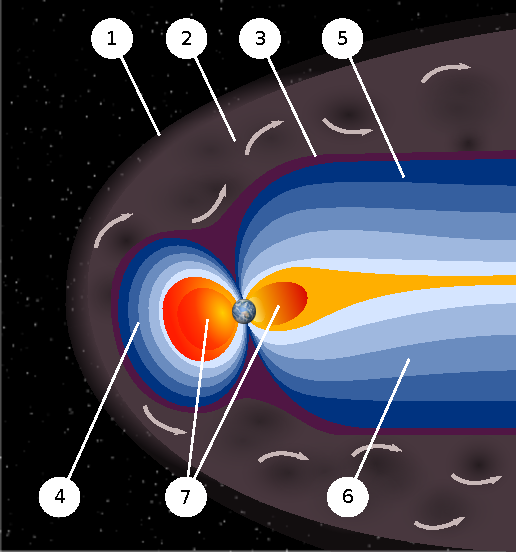
\includegraphics[width=1\textwidth]{figures/chap1/Magnetosphere_Levels.pdf}
                \caption[Earth's Magnetosphere's structure]{Artistic rendition of Earth's magnetosphere, its structure and different layers. The name of each numbered layer is 1.bow shock, 2. magnetosheath, 3. magnetopause, 4. magnetosphere, 5 and 6. tail lobes, 7. plasmasphere.\protect\footnotemark}
                \label{fig:ms_earth}
            \end{center}
        \end{figure}
        \footnotetext{Picture credit: https://commons.wikimedia.org/wiki/File:Magnetosphere\_Levels.svg}

    \section{Studying Space Plasmas} \label{sec:plas3}

        In the previous section (\Cref{sec:plas2}) we discussed two different kinds of naturally
        occurring plasma regions close to Earth. A complete theory of plasma would require us to
        understand the commonality as well as the uniqueness of each of these regions. Consequently,
        over the last century or so the scientific community has devised several methods to study
        them. From Guglielmo Marconi using an antenna on a kite to receive radio signals in 1901 to
        NASA launching a spacecraft costing more than a billion dollars (Parker Solar Probe (PSP))
        in 2018 to study the Sun from a closer distance than ever before, the community has been in
        a constant pursuit to understand them. 
        %\Cref{tab:spcmsn} lists out some of the major programs and missions along with mission
        %objectives, dedicated to such studies.\\
        %\begin{table}[ht] \centering \caption[Major space missions to study space plasmas]{Some of
        %    the major space missions to study space %plasmas \todo{update the table with full
        %    list}} \begin{tabular}{ | p{0.15\linewidth} | p{0.15\linewidth} | p{0.45\linewidth}|}
        %    \hline Spacecraft & Years Active & Major Objective \\
        %        \hline Voyager 1 \newline Voyager 2 & 1977 - \newline 1977 - & Study outer planets
        %         and interplanetary %medium \\
        %        \hline Wind & 1994 - & Study plasma processes in the solar wind near earth and in
        %        magnetosphere and %ionosphere\\
        %        \hline Helios A \newline Helios B & 1974 - 1982 \newline 1976 - 1985 & Observation
        %        of solar wind, electromagnetic fields, cosmic rays\\
        %        \hline MMS & 2016 - & Understanding magnetic reconnection and turbulence\\
        %        \hline Parker Solar Probe & 2018 - & Understanding Coronal heating\\
        %        \hline SoHo & 2018 - & Understanding Coronal heating\\
        %        \hline Ace & 2018 - & Understanding Coronal heating\\
        %        \hline STEREO & 2018 - & Understanding Coronal heating\\
        %        \hline \end{tabular} \label{tab:spcmsn} \end{table}

    \section{In This Thesis} \label{sec:plas4}

        Work done towards this thesis presents an incremental contribution towards understanding the
        nature and behaviour of space plasmas. \Cref{chap:chap2,chap:chap3} provide a theoretical
        background on plasma microkinetics and turbulence, respectively. \Cref{chap:chap4} gives a
        brief overview of all the datasets used in the present document and explains some of the
        data analysis techniques employed in \Crefrange{chap:chap5}{chap:chap7}.

        \Crefrange{chap:chap5}{chap:chap8} report the author's original work. \Cref{chap:chap5}
        discusses the intermittency in space plasmas and simulations as well as its co-development
        with linear instabilities. \Cref{chap:chap6} explores the heating of ions close to the Sun
        as a consequence of intermittent structures. \Cref{chap:chap7} discusses the competition
        between linear and non-linear processes using a statistical approach on six different
        datasets. \Cref{chap:chap8} presents an exploratory study of magnetic field reconstruction
        using machine learning (ML) techniques. \Cref{chap:chap9} provides a summary of the entire
        thesis and a guide for future work.    % This file (chap1.tex) contains the text
                   % for Chapter 1.

%\newpage\null\thispagestyle{empty}

%
% This is Chapter 2 file (chap2.tex)
%
\chapter{Kinetic theory and linear microkinetic instabilities}\label{chap:chap2}

    Kinetic theory forms a significant part of our understanding of plasma, specially at small
    scales (less than a $d_{\rm i}$). In this chapter, we give a brief overview of the salient
    properties of this theory. In \Cref{sec:intr2} we start with the equation of motion for a
    charged particle in an electromagnetic field and extend this idea to an ensemble of particles.
    In \Cref{sec:instab} we discuss anisotropy and linear instabilities arising because of it. We
    also discuss how one can compute rate of growth of these instabilities using kinetic theory. In
    \Cref{sec:app2} we discuss some of the application and observational evidence of linear theory.
    We finish this chapter with a brief discussion of limitations of linear theory in
    \Cref{sec:conc2}.

    \section{Introduction to Plasma Kinetic Theory} \label{sec:intr2}

        \subsection{Equations of motion}\label{sec:eqom}

            Consider a system which consists of a single charged particle of mass $m$ and charge $q$
            in a magnetic field $\mathbf{B}$ and an electric field $\mathbf{E}$. The
            non-relativistic equation of motion for this particle can then be written as:
            \begin{align}
                m \frac{d\mathbf{v}_1}{dt} & = q\left(\mathbf{E} + \mathbf{v}_1 \times \mathbf{B}\right) \label{eq:emot1}
            \end{align}
            and the its exact phase space\index{phase space} density at any point in space can be written as :
            \begin{align}
                \mathcal{F}_1(\mathbf{x},\mathbf{v},t) & = \delta \left(\mathbf{x}-\mathbf{x}_1(t)\right)\delta \left(\mathbf{v}-\mathbf{v}_1(t)\right) \label{eq:dens1}
            \end{align}
            where $\mathbf{x}_1(t)$ and $\mathbf{v}_1(t)$ are the position and velocity of the
            particle at any time $t$ and $\delta(...)$ is the Dirac delta function. The six
            dimensional space spanned by $\mathbf{x}$ and $\mathbf{v}$ is called phase
            space\footnote{Note: $\mathbf{x}$ and $\mathbf{v}$ are independent coordinates in phase
            space.}. If we have $n$ such particles in the system, then for the $i^\mathrm{th}$
            particle, \Cref{eq:emot1} can be written as :
            \begin{align}
                m_{\rm i} \frac{d\mathbf{v}_{\rm i}}{dt} & = q_{\rm i}\left(\mathbf{E}_\mu + \mathbf{v}_{\rm i} \times \mathbf{B}_\mu\right) \label{eq:emotn}
            \end{align}
            where the subscript $\mu$ represents the superposition of all the fields exerted by the
            particles in the system at the position of $i^\mathrm{th}$ particle. The total phase
            space density can now be written as:
            \begin{align}
                \mathcal{F}_{\rm n}(\mathbf{x},\mathbf{v},t) & = \sum_{i=1}^{n}\delta \left(\mathbf{x}-\mathbf{x}_{\rm i}(t)\right)\delta \left(\mathbf{v}-\mathbf{v}_{\rm i}(t)\right) \label{eq:densn}
            \end{align}
            In a closed system where there is no addition or removal of any particle, the total
            phase space density of a fluid element in phase space will remain constant in time.
            Using this conservation of phase space density one can write:
            \begin{align}
                \frac{d}{dt}\left(\mathcal{F}_{\rm n}(\mathbf{x},\mathbf{v},t)\right) & = 0 \label{eq:cons}
            \end{align}
            Since both $\mathbf{x}$ and $\mathbf{v}$ depend on time, we can use the chain rule and
            write \Cref{eq:cons} as:
            \begin{align}
            \frac{\partial \mathcal{F}_{\rm n}}{\partial t} + \frac{d \mathbf{x}}{d t} \cdot \frac{d \mathcal{F}_{\rm n}}{d \mathbf{x}} + \frac{d \mathbf{v}}{d t} \cdot \frac{d \mathcal{F}_{\rm n}}{d \mathbf{v}} & = 0 \label{eq:cons2}
            \end{align}
            where $\frac{\partial}{\partial t}$ is the partial derivative with respect to $t$. In
            \Cref{eq:cons2} we have dropped $(\mathbf{x},\mathbf{v},t)$ for the sake of readability.
            Using the fact that $\frac{d}{d t}\mathbf{x}=\mathbf{v}$ and substituting for $\frac{d
            \mathbf{v}}{d t}$ from \Cref{eq:emotn} in \Cref{eq:cons2}, we have:
            \begin{align}
            \frac{\partial \mathcal{F}}{\partial t} + \mathbf{v} \cdot \nabla_{\mathbf{x}} \mathcal{F} + \frac{q}{m}\left(\mathbf{E}_\mu + \mathbf{v} \times \mathbf{B}_\mu\right) \cdot \nabla_{\mathbf{v}} \mathcal{F} & = 0 \label{eq:cons3}
            \end{align}
            Solving \Cref{eq:cons3} (called the Klimontovich-Dupree equation) is quite a difficult
            task since it contains all the microscopic fields, the computation of which involves
            tracking the position and velocity of all the particles, which as we have already
            discussed is quite impossible to implement. This problem can be mitigated by writing the
            phase density as a sum of two parts, average and fluctuating as below:
            \begin{align}
                \begin{split}
                    \mathcal{F} & = \left<\mathcal{F}\right> + \delta\mathcal{F} \label{eq:pd1}\\
                    & = \mathnormal{f} + \delta\mathcal{F}
                \end{split}
            \end{align}
            where $\left<\mathcal{F}\right>$ denotes the smoothed average or the background value of
            $\mathcal{F}$, and $\delta \mathcal{F}$ is the fluctuation in the smoothed
            $\mathcal{F}$.  For ease of writing, from now on $\left<\mathcal{F}\right>$ will simply
            be denoted by $\mathnormal{f}$, which is also called the distribution function\index{distribution function} and is
            interpreted as the probability of finding a particle at any location within a phase
            space volume d\textbf{x}d\textbf{v}. If we carry out the same process for the fields, we
            can write them as:
            \begin{align}
                \begin{split}
                    \mathbf{E}_{\mu} & = \left<\mathbf{E}_{\mu}\right> + \delta\mathbf{E}_{\mu} \\
                    & = \mathbf{E} + \delta\mathbf{E}_{\mu}
                \end{split}
                \begin{split}
                    \mathbf{B}_{\mu} & = \left<\mathbf{B}_{\mu}\right> + \delta\mathbf{B}_{\mu} \\
                    & = \mathbf{B} + \delta\mathbf{B}_{\mu}\label{eq:pd2}
                \end{split}
            \end{align}
            Since $\mathcal{F}$, \textbf{B} and \textbf{E} are all smoothed averages, their
            fluctuations $(\delta\mathcal{F}, \delta\mathbf{B}, \delta\mathbf{E}$) will form an
            statistical ensemble which would imply that $\left<\delta ... \right> = 0$.

            Using \Cref{eq:pd1,eq:pd2} in \Cref{eq:cons3} and then taking the ensemble average, we
            have:
            \begin{align}
                \frac{\partial \mathnormal{f}}{\partial t} + \mathbf{v} \cdot \nabla_{\mathbf{x}}\mathnormal{f} + \frac{q}{m}\left(\mathbf{E} + \mathbf{v} \times \mathbf{B}\right) \cdot \nabla_{\mathbf{v}} \mathnormal{f} & = \frac{q}{m}\left<\left(\delta\mathbf{E} + \mathbf{v} \times \delta \mathbf{B}\right) \cdot \nabla_{\mathbf{v}} \mathcal{F}\right> \label{eq:kint}
            \end{align}
            This is the kinetic equation and defines the evolution of phase space density with time
            and position.

            Computing the right hand side of \Cref{eq:kint} is quite a difficult task, thus we often
            assume that the correlation between the background field and its fluctuation is
            infinitely small and collisions between particles account for correlation among
            themselves and occur uncorrelated of each other as random events, a consequence of the
            molecular chaos hypothesis\index{chaos hypothesis} (or
            \discolorlinks{\href{https://en.wikipedia.org/wiki/Boltzmann\_equation\#The\_collision\_term\_(Stosszahlansatz)\_and_molecular\_chaos}{\textit{sto\ss
            zahlansatz}}}) \citep{ClerkMaxwell1867}. Under these assumptions we can simply replace
            the right side of \Cref{eq:kint} with a collision operator\index{collision operator}, $\left(\frac{\partial
            \mathnormal{f}}{\partial t}\right)_{\rm c}$, which ideally will have all the information
            related to particle-particle interaction. \Cref{eq:kint} can thus be re-written as:
            \begin{align}
                \frac{\partial \mathnormal{f}}{\partial t} + \mathbf{v} \cdot \nabla_{\mathbf{x}}\mathnormal{f} + \frac{q}{m}\left(\mathbf{E} + \mathbf{v} \times \mathbf{B}\right) \cdot \nabla_{\mathbf{v}} \mathnormal{f} & = \left(\frac{\partial \mathnormal{f}}{\partial t}\right)_{\rm c} \label{eq:bolt}
            \end{align}
            This is the well known Boltzmann equation from statistical mechanics.
            \citet{Baumjohann1996} and references therein give some details about different
            functional forms of collisional operators\index{collision operator}.
            
            Presence of collision can significantly alter the shape of a VDF (see \Cref{sec:dfd} for
            definition). Since collisions can often result in transfer or exchange of energy and
            momentum between particles they work to erode the non-equilibrium features of a VDF
            (more on this later). In a fully ionized plasma where collisions are primarily coulombic
            in nature, computing the collision operator is further complicated by its dependence on
            temperature and density \citep{Baumjohann1996}. \citet{Landau1936} computed the
            collision operator, $\left(\frac{\partial \mathnormal{f}}{\partial t}\right)_{\rm c}$,
            for such a plasma, though solving it even for the simplest of cases is quite a daunting
            ask \citep{Verscharen2019}. However, \citet{Marsch1982, Marsch2010} showed that for
            space plasmas in the inner heliosphere collisions play negligible to minor role. We thus
            simply set the value of collision operator to zero and the Boltzmann equation
            (\Cref{eq:bolt}), in the absence of collision reduces to the Vlasov\index{Vlasov!equation} equation:
            \begin{align}
                \frac{\partial \mathnormal{f}}{\partial t} + \mathbf{v} \cdot \nabla_{\mathbf{x}}\mathnormal{f} + \frac{q}{m}\left(\mathbf{E} + \mathbf{v} \times \mathbf{B}\right) \cdot \nabla_{\mathbf{v}} \mathnormal{f} & = 0 \label{eq:vlas}
            \end{align}
            This equation forms the basis of much of kinetic theory for space plasmas and is used
            extensively in this thesis. We also use the Vlasov equation to derive the dispersion
            relation (see\,\Cref{sec:dpr}), which gives us an idea about the kind of waves and
            instabilities present in the system (more on this later).

        \subsection{Distribution Function and Other Definitions} \label{sec:dfd}

            As discussed in \Cref{sec:eqom}, $\mathnormal{f}(\mathbf{x,v},t)$ gives the probability
            density function (PDF)\index{distribution function!PDF} of particles in phase space. Different statistical moments of the
            PDF gives us macroscopic properties of the whole ensemble. Often, we are interested in
            the behaviour of the system at one particular position in the configuration space at any
            given time. This would mean that the PDF will have no dependence on the position
            (\textbf{x}) or any explicit dependence on time (t). We thus have a PDF with explicit
            dependence on just the velocity given as $\mathnormal{f}(\mathbf{v})$. This is referred
            to as velocity distribution function (VDF)\index{distribution function!VDF}. 

            For a VDF we can define some parameters associated with plasma using its statistical
            moments.\\
            \textbf{Density ($n_{\rm j}$)}: Number density of species $j$, usually expressed in the
            units of $\mathrm{cm^{-3}}$ and can be derived from VDF by computing its zeroth order
            moment as follows:
            \begin{align}
                n_{\rm j} = \int_{\forall \mathbf{v}} d^3\mathrm{v} \mathnormal{f}_{\rm j}\left(\mathbf{v}\right) \label{eq:numden}
            \end{align}
            \textbf{Bulk velocity\index{Bulk velocity} ($\mathbf{v}_{\rm j}$)}: The bulk velocity of the species $j$, or
            the mean particle velocity, usually has units of $\mathrm{km/sec}$ and can be derived
            from the VDF's first-order moment:
            \begin{align}
                \mathbf{v}_{\rm j} = \frac{1}{n_{\rm j}}\int_{\forall \mathbf{v}} d^3\mathrm{v} \mathbf{v} \mathnormal{f}_{\rm j}\left(\mathbf{v}\right) \label{eq:blkvel}
            \end{align}
            \textbf{Thermal Speed\index{Thermal Speed} ($w_{\rm j}$)}: It represents the thermal speed of the species j
            and has units of $\mathrm{km/sec}$. It is a measure of thermal energy of species $j$ and
            the value for it can be derived from the VDF's second-order moment:
            \begin{align}
                \mathrm{v}_{\rm j}^2 + 3\,w_{\rm j}^2 = \frac{1}{n_{\rm j}}\int_{\forall \mathbf{v}} d^3\mathrm{v} \mathbf{v}^2 \mathnormal{f}_{\rm j}\left(\mathbf{v}\right) \label{eq:wtherm}
            \end{align}
            For an anisotropic case, where temperature is different along different directions,
            \Cref{eq:wtherm} is computed for each component separately (see \citet[\S
            1.4.1]{Verscharen2019} for a detailed description).\\
            \\
            \textbf{Temperature ($T_{\rm j}$)}: Using the thermal speed, one can define the
            temperature (in units of K) of the species as:
            \begin{align}
                T_{\rm j} & = \frac{m_{\rm j}\,w_{\rm j}^2}{2k_{\rm B}} \label{eq:temp}
            \end{align}
            In a magnetized plasma, the VDFs commonly exhibit distinct temperatures perpendicular
            and parallel to the magnetic field because of the slightly different heating or cooling
            rates in different directions \citep{Stix1992, Gary1993}. We thus have different
            temperatures in parallel ($T_{\rm \parallel j}$) and perpendicular ($T_{\rm \perp j}$)
            directions and the total temperature of species j is then given as:
            \begin{align}
                 T_{\rm j} = \frac{T_{\rm \parallel j} + 2 T_{\rm \perp j}}{3} \label{eq:ttemp}
            \end{align}
            The ratio of two temperatures (perpendicular and parallel) is called anisotropy\index{anisotropy} and is
            expressed as:
            \begin{align}
                 R_{\rm j} = \frac{T_{\rm \rm \perp j}}{T_{\rm \parallel j}} \label{eq:aniso}
            \end{align}
            \textbf{Parallel Beta ($\beta_{\rm \parallel j}$)}: It is the ratio of parallel thermal
            energy of a species to the magnetic pressure energy stored in the field.
            \begin{align}
                \beta_{\rm \parallel j} = \frac{n_{\rm j}\,k_{\rm B}\,T_{\rm \parallel j}}{B_0^2/(2\mu_\circ)} \label{eq:beta}
            \end{align}
            As we will see later in this chapter (see \Cref{sec:instab2}) the values of parameters
            $R_{\rm j}$ and $\beta_{\rm \parallel j}$ play an important role in determining if a
            region of plasma is stable or unstable. \\
            \\
            \textbf{Shape of a VDF}:\\
            In general the VDF can take a variety of forms as long as they conform to the laws of
            probability. For a plasma in local thermodynamic equilibrium, it takes the shape of a
            Maxwellian distribution\index{distribution function!Maxwellian} as shown in \Cref{eq:vdf}.
            \begin{align}
                \mathnormal{f}_{\rm j}(\mathbf{v}) & = \frac{n_{\rm j}}{\left(\pi w_{\rm j}^2\right)^{3/2}} \mathrm{exp}\left(-\frac{\left|\mathbf{v} - \mathbf{v}_{\rm 0}\right|^2}{w_{\rm j}^2}\right) \label{eq:vdf}
            \end{align}
            where $\mathbf{v}_{\rm 0}$ is the streaming velocity of the plasma. Each species ($j$)
            in the plasma has its own VDF, the statistical moments of which give the species' bulk
            parameters (e.g., density and velocity).

            One can define a direction based on the background field present in the plasma. If we
            assign the direction along the magnetic field as the parallel direction (represented by
            $\parallel$) and the other two orthogonal directions as the perpendicular direction
            (represented by $\perp$), the total magnetic field can be expressed in this new
            coordinate system as:
            \begin{align}
                \mathbf{B} = B_\parallel\,\mathbf{\hat{e}}_\parallel + B_\perp\,\mathbf{\hat{e}}_\perp \label{eq:newdir}
            \end{align}
            where $\mathbf{\hat{e}}_\parallel~\mathrm{and}~\mathbf{\hat{e}}_\perp$ are the unit
            vectors along and perpendicular to the magnetic field.

            It is often easier to work with VDFs in this coordinate system, thus we rewrite
            \Cref{eq:vdf} for a species $j$ in the new coordinate system as:
            \begin{align}
                \mathnormal{f}_{\rm j}(\mathbf{v}) & = \frac{n}{\pi^{3/2} w_{\rm \perp j}^2 w_{\rm \parallel j}} \mathrm{exp}\left(-\frac{(\mathrm{v}_\parallel - \mathrm{v}_{\rm \parallel 0j})^2}{w_{\rm \parallel j}^2} -\frac{|\mathbf{v}_\perp - \mathbf{v}_{\rm \perp 0j}|^2}{w_{\rm \perp j}^2}\right) \label{eq:vdf2}
            \end{align}
            The values of $\mathbf{v}_{\rm \parallel 0j}$ and $\mathbf{v}_{\rm \perp 0j}$ are often
            different resulting in a slightly different VDF in the two directions. For such a case,
            the VDF is referred to as the bi-Maxwellian\index{distribution function!bi-Maxwellian} distribution.
            
            Though in this thesis we use \Cref{eq:vdf2} as the standard/default VDF unless otherwise
            stated, it must be noted that for solar wind, especially at 1\,au, the VDF departs
            significantly from a simple bi-Maxwellian \citep{Feldman1974, Feldman1974a, Marsch1982b,
            Alterman2018}. Ion VDFs often have an asymmetry which can be more accurately accounted
            for by superposition of a differentially flowing bi-Maxwellian \citep{Alterman2018}.
            Other forms of distribution such as kappa distribution has also been used to study the
            non-Maxwellian features of VDF like enhanced tail \citep{Pierrard2010,Pierrard2014,
            Maksimovic1997,Nicolaou2020}.

    \section{Linear Microkinetic Instabilities} \label{sec:instab}

        \subsection{The Linear Dispersion Relation} \label{sec:dpr}
 
            Though in \Cref{sec:eqom} we made several assumptions and used our a priori knowledge of
            the system, solving \Cref{eq:vlas} for even a simple distribution like the bi-Maxwellian
            (\Cref{eq:vdf2}) is quite complicated and computationally expensive. Coupling between
            fields produced by one species with another species complicates it further.
            Linearization (or linear analysis), where one assumes plain wave perturbation in fields
            and the VDF helps simplify the problem while keeping the underlying physics of the
            equations intact as long as the fluctuations have small amplitude relative to the
            background values. In standard linear theory, we assume an equilibrium (i.e., constant)
            background and perturb it with a small-amplitude sinusoidal fluctuation of wave vector
            \textbf{k} and angular frequency $\omega$. The goal then is to derive, for a given
            plasma, the dispersion relation: the relationship between \textbf{k} and $\omega$. Under
            this assumption one can rewrite \Cref{eq:pd1,eq:pd2} as:
            \begin{align}
                \begin{split}
                    \mathnormal{f}_{\rm j}(\mathbf{x}, \mathbf{v}, t) & = \mathnormal{f}_{\rm j}^0(\mathbf{x}, \mathbf{v}) + \mathnormal{f}_{\rm j}^1(\mathbf{x}, \mathbf{v}, t)\\
                    & = \mathnormal{f}_{\rm j}^0(\mathbf{x}, \mathbf{v}) + \mathnormal{f}_{\rm j}^1(\mathbf{k}, \omega, \mathbf{v})~e^{(i(\mathbf{k}\cdot \mathbf{x} -\omega t))}\label{eq:vdfn1}
                \end{split}
            \end{align}
            \vspace{-0.4cm}
            \begin{align}
                \begin{split}
                    \mathbf{B}(\mathbf{x}, t) & = \mathbf{B}^0(\mathbf{x}) + \mathbf{B}^1(\mathbf{x}, t)\\
                    & = \mathbf{B}^0(\mathbf{x}) + \mathbf{B}^1(\mathbf{k},\omega)~e^{(i(\mathbf{k}\cdot \mathbf{x} -\omega t))}\label{eq:mag1}
                \end{split}
            \end{align}
            \vspace{-0.4cm}
            \begin{align}
                \begin{split}
                    \mathbf{E}(\mathbf{x}, t) & = \mathbf{E}^0(\mathbf{x}) + \mathbf{E}^1(\mathbf{x}, t)\\
                    & = \mathbf{E}^0(\mathbf{x}) + \mathbf{E}^1(\mathbf{k},\omega)~e^{(i(\mathbf{k}\cdot \mathbf{x} -\omega t))}\label{eq:efl1}
                \end{split}
            \end{align}
            Where $\mathbf{k}$ and $\omega$ are the wavenumber vector and the frequency of
            perturbation, respectively. \Crefrange{eq:vdfn1}{eq:efl1} along with Maxwell's
            equation's (\Crefrange{eq:maxwell1}{eq:maxwell4}) help us drive the dispersion
            relations. In order to do so, we start with some simple assumptions and conditions. We
            work in a frame of reference where the zeroth order current density
            ($\mathbf{J}^0(\mathbf{x})$) and electric field ($\mathbf{E}^0(\mathbf{x})$) are zero
            and the magnetic field ($\mathbf{B}^0(\mathbf{x})$) is constant. Thus
            \Cref{eq:mag1,eq:efl1} can be rewritten as:
            \begin{align}
                \mathbf{B}(\mathbf{x}, t) & = \mathbf{B}_{\rm 0} + \mathbf{B}^1(\mathbf{x}, t)\label{eq:mag2}\\
                \mathbf{E}(\mathbf{x}, t) & = \mathbf{E}^1(\mathbf{x}, t)\label{eq:efl2}\\
                \mathbf{J}(\mathbf{x}, t) & = \mathbf{J}^1(\mathbf{x}, t)\label{eq:curr2}
            \end{align}
            We choose a co\"ordinate system with $z$-axis along the background magnetic field
            ($\mathbf{B}_{\rm 0}$). The angle between the direction of propagation of fluctuation
            ($\mathbf{k}$) and the magnetic field is:
            \begin{align}
                \cos \left(\theta \right) & = \frac{\mathbf{k}\cdot\mathbf{B}}{k B}\label{eq:theta}
            \end{align}
            Substituting expressions for $\mathbf{J}, \mathbf{B}~\mathrm{and}~\mathbf{E}$ into
            Maxwell's equations (\Crefrange{eq:maxwell1}{eq:maxwell4}) and simplifying we have:
            %by substituting $\frac{\partial}{\partial t}$ with $\omega$ and $\nabla$ with
            %$\mathbf{k}$, we get:
            \begin{align}
                \mu_\circ\,\mathbf{J}^1(\mathbf{k}, \omega) & = \frac{i}{\omega}\,\mathbf{k} \times \left[\mathbf{k} \times \mathbf{E}^1(\mathbf{k}, \omega)\right] + \frac{i\,\omega}{c^2}\,\mathbf{E}^1(\mathbf{k}, \omega) \label{eq:curr3}
            \end{align}
            In similar fashion to the particle velocity in \Cref{eq:blkvel} one can write the flux
            density as:
            \begin{align}
                \Gamma_{\rm j}^1(\mathbf{k}, \omega) = \int_{-\infty}^{\infty}d^3 v\,\mathbf{v}\,\mathnormal{f}_{\rm j}^1(\mathbf{k}, \omega, \mathbf{v}) \label{eq:flux1}
            \end{align}
            and thus define the current density as:
            \begin{align}
                \mathbf{J}^1(\mathbf{k}, \omega) & = \sum_{\rm j} q_{\rm j}\,\mathbf{\Gamma}_{\rm j}^1(\mathbf{k}, \omega) \label{eq:curr4}
            \end{align}
            For species $j$ we can define the dimensionless conductivity tensor $\mathbf{S}_{\rm j}$
            as:
            \begin{align}
                \mathbf{\Gamma}_{\rm j}^1(\mathbf{k}, \omega) & = - \frac{i\,\epsilon_\circ\,k^2\,c^2}{q_{\rm j}\,\omega}\,\mathbf{S}_{\rm j}(\mathbf{k},\omega)\cdot \mathbf{E}^1(\mathbf{k},\omega) \label{eq:curr5}
            \end{align}
            Combining \Cref{eq:curr2,eq:curr3,eq:curr4} gives us:
            \begin{align}
                \mathbf{D}(\mathbf{k},\omega)\cdot \mathbf{E}^1(\mathbf{k},\omega) & = 0 \label{eq:disp1}
            \end{align}
            where,
            \begin{align}
                \mathbf{D}(\mathbf{k},\omega) = \left(\omega^2 - c^2\,k^2\right)\mathbf{I} + c^2\,\mathbf{k}\,\mathbf{k} + c^2\,k^2\,\sum_{\rm j}\,\mathbf{S}_{\rm j}(\mathbf{k},\omega) \label{eq:disp2}
            \end{align}
            with \textbf{I} being the 3-dimensional identity matrix and \textbf{k}\,\textbf{k} being
            the dyadic\footnote{The dyadic product between two vectors \textbf{a} and \textbf{b} is
            simply the product between the vector and its transpose, so one has
            $\mathbf{a}\,\mathbf{b} = \mathbf{a}\,\mathbf{b}^T$, which results in a rank-two
            tensor.} product of the wavevector. For \Cref{eq:disp2} to be true, $\mathbf{E}^1$
            cannot be allowed to go to zero since that would allow perturbations in the system to
            vanish. Hence we must have the determinant of $\mathbf{D}(\mathbf{k},\omega)$ go to
            zero, thus:
            \begin{align}
                \mathrm{det}(\mathbf{D}(\mathbf{k},\omega)) & = 0 \label{eq:disp3}
            \end{align}
            which is the plasma dispersion relation\index{dispersion relation}. \citet{Gary1993} notes that this equation can
            be solved ``either as a boundary value problem ($\omega$ is given as real, one solves
            for a complex component of $\mathbf{k}$) or as an initial value problem ($\mathbf{k}$ is
            given as real, one solves for complex $\omega$)''.
            
            \Cref{eq:disp3} in general gives infinite number of solutions for $\omega$ for any value
            of \textbf{k} and a set of plasma parameters. Thus $\omega (\mathbf{k})$ is a multi
            valued function with multiple branches corresponding to different modes (see
            \citet[Figure 2]{Schwartz1980}). However most modes are strongly damped and thus
            dissipate before they can substantially effect the plasma.

        \subsection{Temperature Anisotropy Induced Instabilities} \label{sec:instab2}

            In a homogeneous plasma (PDF is independent of position) in local thermodynamic
            equilibrium (LTE), all fluctuations (at any \textbf{k} and $\omega$) are damped and thus
            have a decaying amplitude. However, departure from LTE because of the non-Maxwellian
            properties of VDFs (temperature anisotropy or relative drift between two different
            species, etc.) introduce free energy into the system. This results in circumstances
            where instead of getting damped some perturbations grow exponentially and make the
            system unstable. The rate at which such a perturbation propagates and gets damped or
            grows is computed by solving the dispersion relation (\Cref{eq:disp3}). Solutions of
            \Cref{eq:disp3} using the initial value problem method gives $\omega$, which is in
            general complex and can be written as:
            \begin{align}
                \omega = \omega_{\rm r} + i \gamma \label{eq:omega}
            \end{align}
            where, $\omega_{\rm r}$ is the real component and $\gamma$ is the damping rate ($\gamma
            < 0$) or growth rate\index{microinstability!growth rate} ($\gamma > 0$). In the presence of a growth rate, the fluctuations
            present in the system start to grow exponentially. If the process continues,
            fluctuations start having amplitudes comparable to the background value, which makes the
            assumption of linearity void and makes the system non-linear. The state of the system
            can no longer be predicted by linear theory and instead relies on non-linear dynamics.

            When an instability has $\gamma = 0$ for any wave vector, we call it threshold\index{threshold} of the
            associated instability. We also define $\gamma_{\max}$ for a given branch of dispersion
            solutions as the maximum value of $\gamma$ for different wavenumbers ($\mathbf{k}$) and
            for all propagation directions ($\theta$). $\omega_{max}$ and $\mathbf{k}_{\max}$ are
            then defined as the values of $\omega$ and $\mathbf{k}$ corresponding to $\gamma =
            \gamma_{\max}$ respectively. Mathematically this can be written as:
            \begin{align}
                \begin{split}
                    \gamma_{\max}^j = \mathrm{\max}\left(\gamma^j\left(\mathbf{k},\theta\right)\right)~~\forall \left(\mathbf{k}, \theta\right) \label{eq:gammamax}
                \end{split}
            \end{align}
            where $j$ represents the branch of dispersion solutions for which $\gamma$ was computed.

            In this thesis we consider ion temperature anisotropy as the only source of free energy.
            For instability driven by ion temperature anisotropy, there are four distinct modes
            depending on the anisotropy value ($R_{\rm p}$) and the direction of propagation
            ($\theta$). For parallel propagation ($\theta=0$), there are two modes: ion cyclotron
            for $R_{\rm p} > 1$ and parallel firehose for $R_{\rm p} < 1$. In the oblique direction
            ($0 < \theta < 90$), the corresponding instabilities are mirror ($R_{\rm p} > 1$) and
            oblique firehose ($R_{\rm p} < 1$). It is worth noting that neither of these two oblique
            instabilities propagate. \Cref{tab:instab} gives a summary of all four instabilities
            discussed.

            \begin{table}[ht]
                \centering
                \caption[Microkinetic instabilities]{List of four temperature-anisotropy induced instabilities in plasma}
                \begin{tabular}{ | p{0.25\linewidth} | p{0.25\linewidth} | p{0.25\linewidth}| }
                    \hline
                    Anisotropy Range & Parallel ($\omega_{\rm r} > 0$) & Oblique ($\omega_{\rm r} =
                    0$)\\
                    \hline
                    $R_{\rm p} > 1$ & Ion cyclotron & Mirror\\
                    \hline
                    $R_{\rm p} < 1$ & Parallel firehose & Oblique firehose\\
                    \hline
                \end{tabular}
                \label{tab:instab}
            \end{table}

        \subsection{Computing Growth Rates}\label{sec:cgr}

            Computation of growth rates ($\gamma$) for any given value of the plasma parameters for
            a given branch of instability means solving \Cref{eq:disp3} for all different values of
            \textbf{k}. This is generally done by using a numerical dispersion solver. This project
            used tables of $\gamma_{\max}$ as a function of the plasma parameters developed by
            \citet{Maruca2012} using the software of \citet{Gary1993}. For our case, given a value
            of $R_{\rm p}$ and $\beta_{\parallel \rm p}$, we check the table for values of ($R_{\rm
            p}, \beta_{\parallel \rm p}$) that are closest to the input value and then use an
            interpolation technique (cubic spline interpolation) to get the value at that exact
            input point.

            Once we get the $\gamma_{\max}$ value corresponding to an instability, we normalize it
            to the cyclotron frequency of protons ($\gamma_{\max} \rightarrow
            \gamma_{\max}/\Omega_{\rm cp}$). However, not all computed values of the growth rate
            will have a significant effect on the plasma dynamics. As is expected if growth rate is
            high, the instability grows faster and conversely it will take the instability a long
            time to manifest or change the dynamics if it has a small growth rate. Thus, one can
            think of $1/\gamma$ as a proxy for the amount of time it will take for the instability
            to manifest itself. For a positive but an infinitesimal value of $\gamma_{\max}$, the
            value of time will be much, much greater than the other characteristic time scales of
            the system, which means the instability will never have time to significantly affect the
            plasma. We thus define a cut-off\index{microinstability!cut-off} value of growth rates, in units of proton cyclotron
            frequency, as:
            \begin{align}
                \gamma_{\max, \mathrm{cut\textrm{-}off}}^j & = 10^{-5}\,\Omega_\mathrm{{cp}} \label{eq:gammacutoff}
            \end{align}
            For any combination of ($R_{\rm p}, \beta_{\parallel \rm p}$) if the value of
            $\gamma_{\max}/\Omega_\mathrm{{cp}}$ is less than $10^{-5}$ we essentially set those
            values to zero and assume that the plasma is completely stable at those points. Choosing
            this cut-off is a bit arbitrary. Different studies have chosen different threshold
            values. For example \citet{Gary1999} and \citet{Gary2006} chose $\gamma =
            10^{-2}\,\Omega_{\rm cp}$ as their cut-off, whereas both \citet{Hellinger2006} and
            \citet{Klein2018} settled on cut-off value of $\gamma = 10^{-3}\,\Omega_{\rm cp}$. As
            long as the cut-off value of $\gamma$ is significantly smaller than that of other
            relevant time scales (see \Cref{sec:nlts,sec:data7}) it can comfortably be set to zero.

    \section{Application of linear theory and observational evidence}\label{sec:app2}

        The low density and extreme dynamics of space plasmas, such as  solar wind and the
        magnetosheath (see \Cref{sec:plas2}), ensure that they almost invariably deviate
        substantially from local thermal equilibrium \citep{Marsch2006a,Verscharen2019}. For
        example, even though the majority of solar wind ions are protons (ionized hydrogen) or
        $\alpha$-particles (fully ionized helium), these two particle species rarely have equal
        temperatures or bulk velocities \citep[see,
        e.g.,][]{Feldman1974a,Marsch1982,Hefti1998,Kasper2008,Maruca2013a}. \Cref{fig:temp_1au}
        shows the distribution of temperature for these two species using data from the Wind
        spacecraft (\Cref{sec:wind} for more details on the dataset used). Furthermore, the VDF of
        any given ion species often significantly departs from the entropically favored Maxwellian
        functional form \citep{Feldman1973a,Feldman1974,Marsch1982b, Alterman2018}. Observations of
        solar wind and magnetosheath from multiple spacecraft
        \citep{Feldman1973b,Marsch1982b,Kasper2002} have shown that the protons exhibit distinct
        kinetic temperatures, $T_{\rm \perp p}$ and $T_{\rm \parallel p}$. Both values of $R_{\rm p}
        > 1$ and $R_{\rm p} < 1$ are commonly observed in the solar wind and in Earth's
        magnetosheath, making it an ideal candidate for the application of linear Vlasov theory\index{Vlasov!linear Vlasov theory}.
        \Cref{fig:aniso_wnd_mms} shows distribution of $R_{\rm p}$ for solar wind at 1\,au and
        magnetosheath.
        \begin{figure}
            \begin{center}
                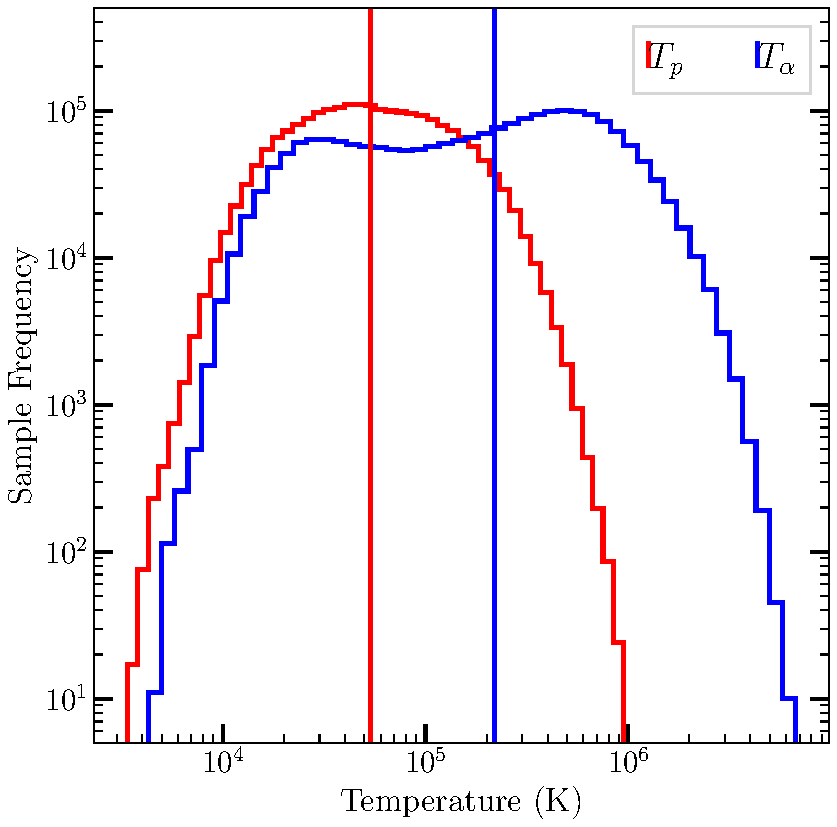
\includegraphics[width=0.55\textwidth]{figures/chap2/proton_alpha_temp_dist_wnd.pdf}
                \caption[Temperature distribution at 1\,au]{Distribution of proton and $\alpha$-temperatures at 1\,au. Vertical lines show the median temperature of each species.}
                \label{fig:temp_1au}
            \end{center}
        \end{figure}

        \begin{figure}
            \begin{center}
                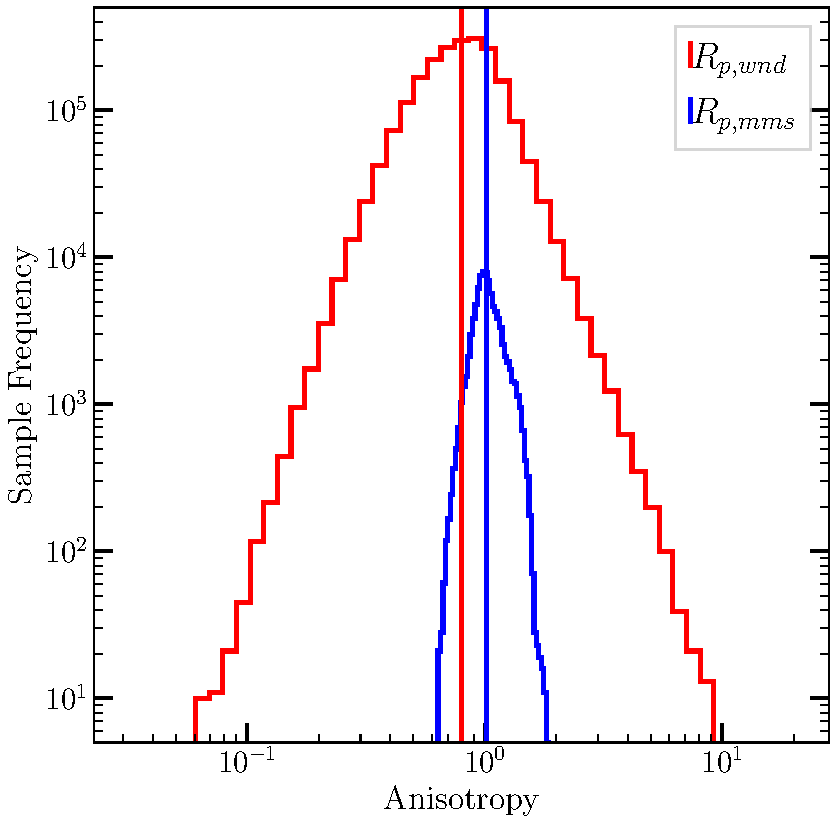
\includegraphics[width=0.55\textwidth]{figures/chap2/proton_aniso_dis_mms_wnd.pdf}
                \caption[$R_{\rm p}$ distribution at 1\,au and in magnetosheath]{Distribution of proton temperature anisotropy at 1\,au (red) and in the magnetosheath (blue). Vertical lines show the median values at each location.}
                \label{fig:aniso_wnd_mms}
            \end{center}
        \end{figure}

        As discussed in \Cref{sec:instab2} if $R_{\rm p}$ departs sufficiently from unity, it can
        trigger a kinetic microinstability\index{microinstability}: a short-wavelength fluctuation with an exponentially
        growing amplitude. The threshold $R_{\rm p}$-value for the onset of a proton
        temperature-anisotropy instability depends on all plasma parameters (e.g., composition and
        relative temperatures), depending most strongly on proton parallel beta ($\beta_{\parallel
        \rm p}$). \Cref{fig:gamma_cntr} shows various thresholds on an ($R_{\rm p}, \beta_{\rm
        \parallel p}$) plane for the four modes of instabilities. As is evident, at fixed $R_{\rm
        p}$ a slight increment in $\beta_{\parallel \rm p}$ can lead to significant increase in the
        growth rate.

        \begin{figure}
            \begin{center}
                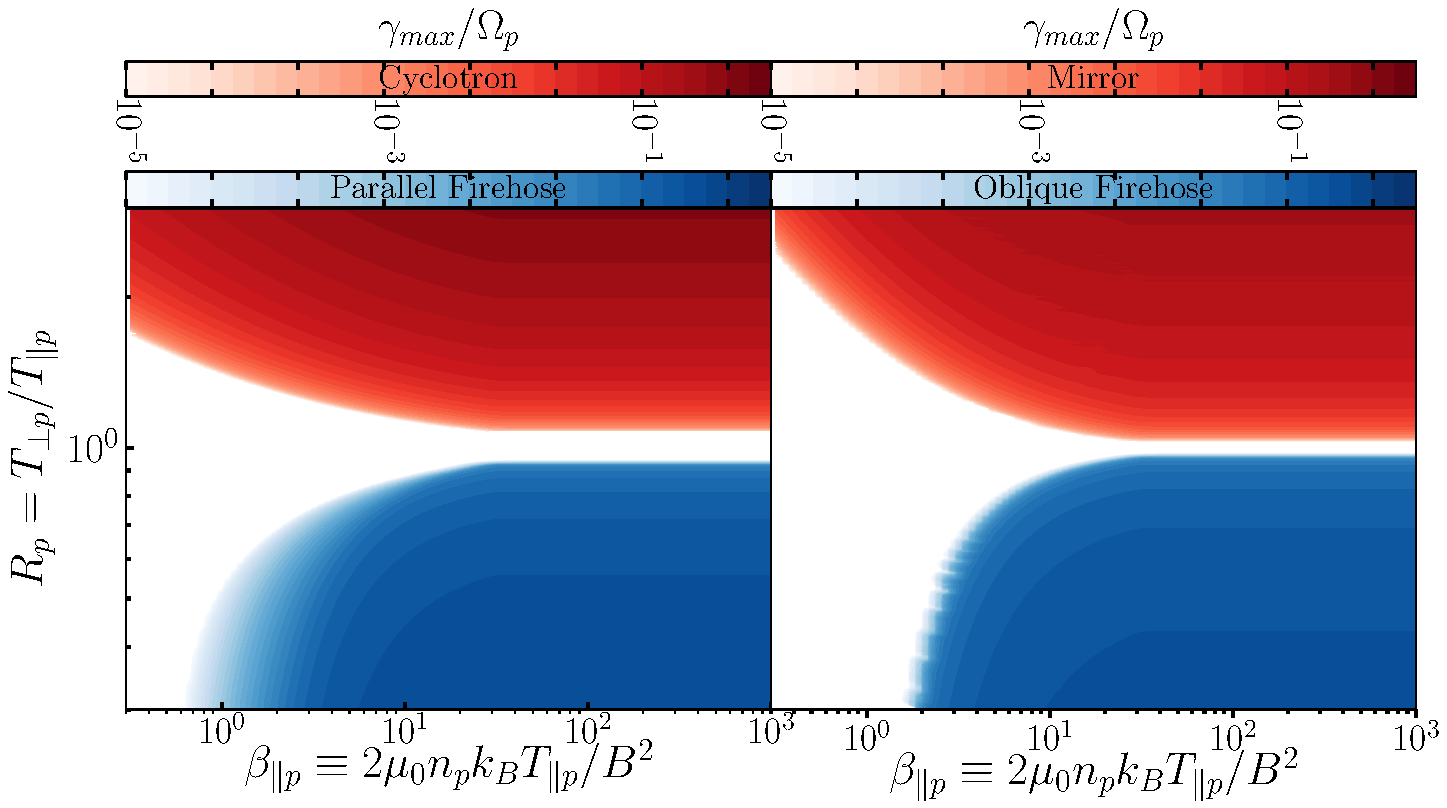
\includegraphics[width=1\textwidth]{figures/chap2/growth_rate_contours.pdf}
                \caption[$\gamma$ Contours]{Contours of constant growth rates.}
                \label{fig:gamma_cntr}
            \end{center}
        \end{figure}

        These instabilities have threshold $R_{\rm p}$-values, which means that they can effectively
        limit the degree to which proton temperature can depart from isotropy. If an unstable mode
        grows and does not saturate, it eventually becomes nonlinear, continues to scatter particles
        in phase space, and eventually drives the VDF toward local thermal equilibrium. Multiple
        studies have analyzed large datasets from various spacecraft and under the assumptions of a
        spatially homogeneous plasma and a bi-Maxwellian proton velocity distribution; such studies
        have found that the joint distribution of $(\beta_{\parallel \rm p},R_{\rm p})$-values from
        the interplanetary solar wind largely conform to the limits set by the instability
        thresholds \citep{Gary2001,Kasper2002,Hellinger2006,Matteini2007}.
        \Cref{fig:brazil_prob_wnd} shows the joint probability distribution of ($R_{\rm p},
        \beta_{\parallel \rm p}$) and the thresholds\index{threshold} corresponding to different instability modes
        for $\gamma_{\max}/\Omega_{\rm cp} = 10^{-2}$ \footnote{Please see \Cref{apdx:A} for more
        details on how these figures were made and how thresholds were computed}. We can see that
        the probability density decreases significantly as one moves closer to any of the threshold
        values. A recent study by \citet{Maruca2018} confirmed the same effect in Earth's
        magnetosheath, which is shown in \Cref{fig:brazil_prob_mms} (see \Cref{apdx:A} for examples
        of a $(\beta_{\parallel \rm p},R_{\rm p})$-plot in other systems). Additional studies have
        found that plasma with unstable $(\beta_{\parallel \rm p},R_{\rm p})$-values is
        statistically more likely to exhibit enhancements in magnetic fluctuations \citep{Bale2009}
        and proton temperature \citep{Maruca2011}. These findings suggest that the instabilities not
        only regulate temperature anisotropy in space plasmas but, in doing so, play an integral
        role in the large-scale evolution of the plasmas.

        \begin{figure}
            \begin{center}
                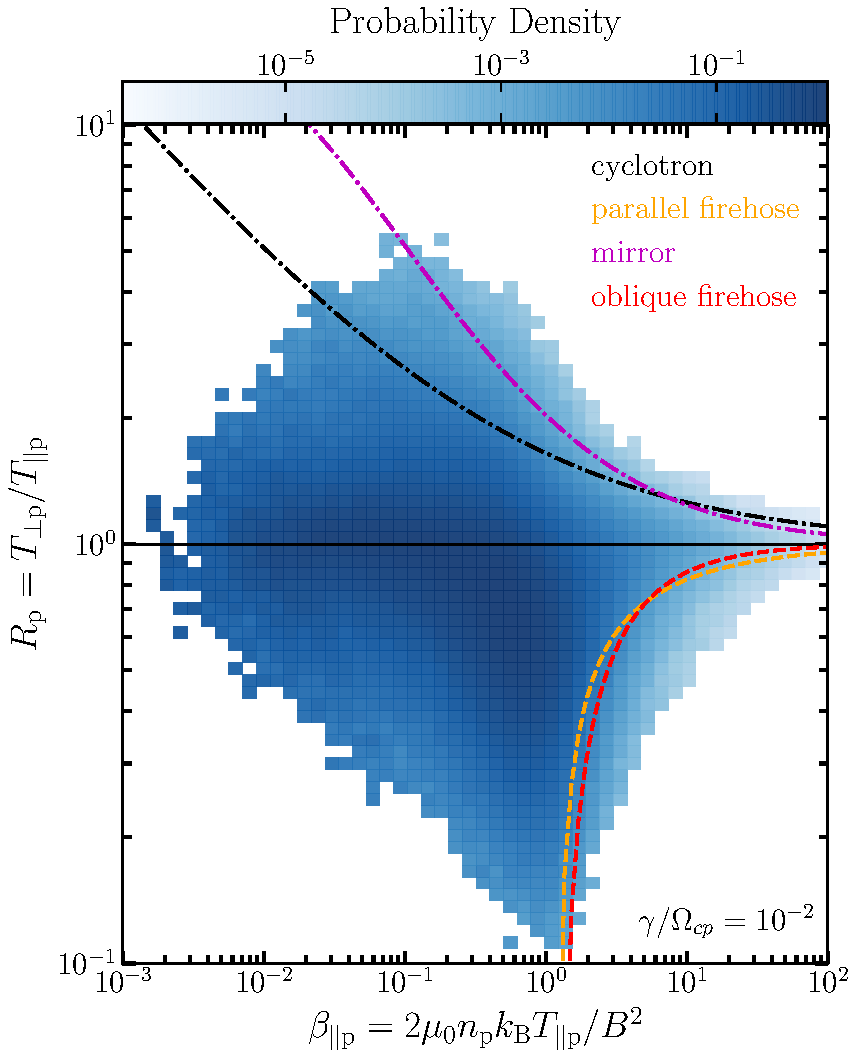
\includegraphics[width=1\textwidth]{figures/chap2/brazil_prob_wnd.pdf}
                \caption[Brazil-plot at 1\,au]{Plot of estimated probability density, $\Tilde{p}$ of
                ($R_{\rm p}, \beta_{\parallel \rm p}$) for solar wind at 1\,au (from \texttt{wnd}
                dataset, see \Cref{chap:chap4}) and thresholds associated with different
                instabilities for threshold value of $\gamma_{\max}/\Omega_{\rm cp} = 10^{-2}$.}
                \label{fig:brazil_prob_wnd}
            \end{center}
        \end{figure}
        \begin{figure}
            \begin{center}
                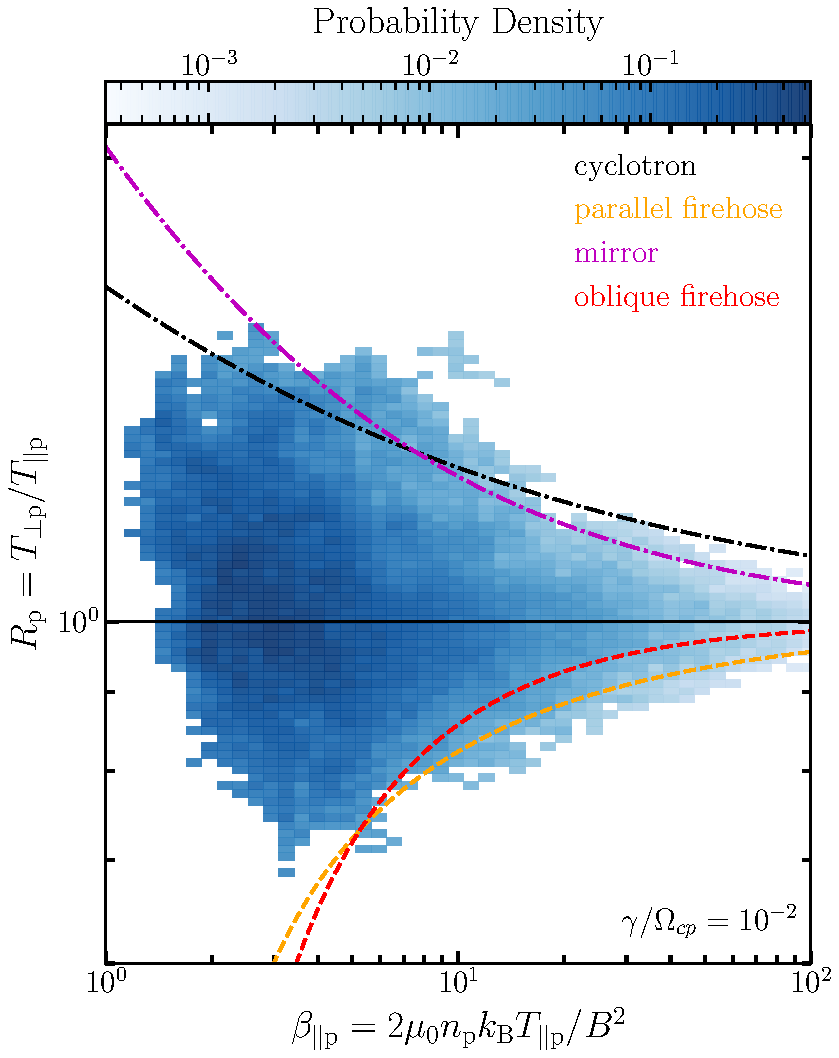
\includegraphics[width=1\textwidth]{figures/chap2/brazil_prob_mms.pdf}
                \caption[Brazil-plot in magnetosheath]{Plot of estimated probability density,
                $\Tilde{p}$ of ($R_{\rm p}, \beta_{\parallel \rm p}$) for Earth's magnetosheath
                (from \texttt{mms} dataset, see \Cref{chap:chap4}) and thresholds associated with
                different instabilities for threshold value of $\gamma_{\max}/\Omega_{\rm cp} =
                10^{-2}$.}
                \label{fig:brazil_prob_mms}
            \end{center}
        \end{figure}

        The empirical studies of $(\beta_{\parallel \rm p},R_{\rm p})$-distributions --- especially
        that by \citet{Matteini2007} --- indicate that the instabilities globally limit proton
        temperature anisotropy and affect the large-scale thermodynamics of expanding solar wind
        plasma. Nevertheless, the instabilities themselves act on far smaller scales. Indeed,
        \cite{Osman2012} found that unstable $(\beta_{\parallel \rm p},R_{\rm p})$-values are
        statistically more likely to exhibit enhanced values of the partial variance of increments
        (PVI)\index{PVI}, which is an indicator of intermittent structure (see \Cref{sec:intmt}). This result
        suggests that long-wavelength turbulence may play a substantial role in generating the local
        plasma conditions that drive these microinstabilities. Also, advancements made in numerical
        simulation by \citet{Servidio2012a, Greco2012, Servidio2015}, with corroboration from space
        plasma observations \citep{Marsch1992, Sorriso-Valvo1999, Osman2011, Osman2012, Kiyani2009}
        show the importance of intermittency in interpretation of these observations. We discuss
        these in more detail in \Cref{chap:chap3}.

    \section{Limitations of linear theory}\label{sec:conc2}

        Though linear theory works well for plasma with a homogeneous background, when it comes to
        its application to study the characteristics of space plasmas, the method is not without
        caveats. Multiple studies have shown space plasma to be highly structured and thus
        inhomogeneous \citep{Burlaga1968, Tsurutani1979, Ness2001, Osman2012, Osman2012a,
        Greco2012}. In fact, by all accounts, inhomogeneity is ubiquitously present in space plasma,
        and thus any study of instabilities in plasma should take into account the inhomogeneity of
        the background among variation in other parameters.

        Consequently, use of linear theory for such studies of course presents a theoretical
        inconsistency in the application of computed instability thresholds\index{threshold} to study the properties
        of plasma because of the underlying disparity between the assumptions of linear theory and
        the observed space plasma. However, several studies over the last three decades have
        presented empirical evidence of agreement between the observations and theoretical
        predictions \citep{Gary1991, Gary1994, Gary2001, Gary2006, Kasper2002, Hellinger2006,
        Maruca2011, Maruca2012, Maruca2018}. These studies strongly suggest that linear instability
        thresholds are indeed efficient in restricting the plasma/plasma VDF in a narrow region of
        ($\beta_{\parallel \rm p}, R_{\rm p}$)-plane, inhibiting the excursion of plasma VDFs to
        extreme anisotropy regions at high $\beta_{\parallel \rm p}$. Although limitations on
        spatial and temporal resolution using present-day spacecraft make it difficult to directly
        demonstrate the existence of such instabilities in space plasmas, work done by,
        \citet{Bale2009, He2011, Podesta2013, Jian2009, Jian2010, Jian2014, Klein2014, Telloni2016,
        Gary2016} among others provide indirect evidence for the presence of various different
        instabilities. More details can be found in \citet{Verscharen2019} and references therein.

        Given these limitations of linear theory and its application, we have to look into the
        non-linear processes and study how those processes affect the dynamics of the plasma.
        \Cref{chap:chap3} introduces some the non-linear processes in plasmas and discusses how they
        affect the dynamics.    % This file (chap2.tex) contains the text
                   % for Chapter 2.

\newpage\null\thispagestyle{empty}

%
% This is Chapter 3 file (chap3.tex)
%
\chapter{Non-linear Plasma Dynamics}\label{chap:chap3}

    \section{Introduction to Turbulence}\label{sec:intr3}

        In laminar flow, different layers of fluid move smoothly without much mixing between layers,
        and the characteristic quantities/parameters - like velocity, pressure, or density - vary
        smoothly in a predictable way. A system where these quantities fluctuate in a chaotic
        fashion is called turbulent and the phenomena is called turbulence\index{turbulence}. Because of the chaotic
        nature of the fluctuations, unlike the laminar flow, prediction of the exact state of the
        system is essentially impossible. This makes a system extremely complicated to study, so
        much so that Sir Horace Lamb once remarked \citep{Goldstein1969}:

        \begin{quote}
             I'm an old man now, and when I die and go to heaven there are two matters on which I
             hope for enlightenment. One is quantum electrodynamics, and the other is turbulent
             motion of fluids. And about the former I'm rather optimistic.
            %\footnote{To be honest as an Indian, I find the idea of a $19^{th}$ century British's
            %assumption that they would go to heaven rather optimistic.}
        \end{quote}

        Turbulence is extremely complicated and the fact that it is ubiquitous in nature (and in
        most man made processes involving fluids) makes it
        unavoidable.%\footnote{Not that we would have avoided it anyway.}.

        Whether a given fluid system will develop turbulence largely depends on its viscosity, which
        is the liquid equivalent of friction and is a measure of how easy it is to for the liquid to
        flow \citep{Chapman1916, Jeans1905} and its Reynolds number
        \citep{Reynolds1883,Reynolds1886,Matthaeus1980}. A small Reynolds number\index{Reynolds number} means that the
        system is laminar whereas a high value Reynolds number implies turbulent flow. For a neutral
        fluid it is defined as:
        \begin{align}
            R_{\rm e} = L \frac{u}{\nu} \label{eq:rnld}
        \end{align}
        where $L$ is the characteristic length of the system, $u$ is the mean flow velocity and
        $\nu$ is the kinematic viscosity. For a similar amount of force or external pressure, a
        highly viscous fluid or one with low $R_{\rm e}$ can maintain laminar flow for much longer
        duration than a fluid with low viscosity or high $R_{\rm e}$. Presence of viscosity in a
        fluid leads to interaction between different layers or scales and results in energy transfer
        from larger to smaller scales through eddies which eventually reaches the smallest scale and
        dissipate as heat \citep{Kolmogorov1941a, Kolmogorov1941} in a process called energy cascade
        in turbulence. In a weakly collisional and magnetized plasma, the presence of charged
        particle and magnetic field complicates the process. For a system like solar wind, the
        situation is further complicated because of the relatively similar size of the system and
        the mean free path\footnote{Mean free path is defined as the average distance travelled by
        particles between two successive collisions.}\citep[Appendix 2]{Echim2010} both of which are
        of the order of 1\,au \citep[Table 1]{Verscharen2019} and thus one cannot use the classic
        methodology developed by \citet{Enskog1917} and \citet{Chapman1918}.

        Turbulence cascade has far reaching consequences for both neutral fluids and plasmas. It
        provides a pathway for the dissipation or transfer of energy from large scales, where they
        can be introduced, to smaller scales. In the next section (\Cref{sec:inter3b}) we will look
        at some of the consequences of turbulence in space plasmas. We discuss only those which are
        relevant to this thesis. In \Cref{sec:nlts} we discuss the linear and non-linear time scales
        associated with their respective phenomena.

    \section{Consequences of Turbulence in Space Plasmas} \label{sec:inter3b}

        In-situ observations and theoretical interpretations have established the ubiquitous
        presence of turbulence in space plasmas \citep[and references
        therein]{Matthaeus2011,Matthaeus2021}. In this section we discuss three of the major
        consequences that arise because of turbulence in space plasmas. Though these three are not
        the only consequences of turbulence, these were selected because of their relevance to this
        thesis, as we will see in \Cref{chap:chap5,chap:chap6,chap:chap7}.

        \subsection{Heating of plasma} \label{sec:hop}

            In space plasmas, under the assumption that the magnetic field changes slowly (slower
            than the ion gyrotropic time scale), the magnetic moment ($\mu$) of the particle is
            conserved \citep{Baumjohann1996,Verscharen2019}. Thus, we can write:
            \begin{align}
                \frac{d \mu}{dt} & = 0 \label{eq:mu_0}
            \end{align}
            where, $\mu = m_{\rm p}\,w_{\rm \perp p}^2/(2B)$, $m_{\rm p}$ is the proton mass,
            $w_{\rm \perp p}^2$ is the perpendicular thermal velocity and $B$ is the magnitude of
            magnetic field. Writing \Cref{eq:mu_0} in terms of the proton-perpendicular temperature
            using \Cref{eq:temp}, we have:
            \begin{align}
                \frac{d}{dt} \left(\frac{k_{\rm B} T_{\rm \perp p}}{B}\right) & = 0 \label{eq:mu_1}
            \end{align}
            or:
            \begin{align}
                T_{\rm \perp p} & \propto B \label{eq:mu_2}
            \end{align}
            In a similar vein for the parallel direction, under the assumption of no dissipation, we
            have:
            \begin{align}
                \frac{d}{dt} \left(\frac{k_{\rm B} T_{\rm \parallel p} B^2}{n_{\rm p}^2}\right) & = 0 \label{eq:mu_3}
            \end{align}
            or:
            \begin{align}
                T_{\rm \parallel p} & \propto \left(\frac{n_{\rm p}}{B}\right)^2 \label{eq:mu_4}
            \end{align}
            These two conservation laws (\Cref{eq:mu_2,eq:mu_4}) for the \textit{double-adiabatic
            invariants} are also called \textit{Chew–Goldberger–Low or CGL invariants} (for a bit
            more detailed discussion and derivation of CGL invariants, see see \Cref{apdx:B}).

            In the inner heliosphere, the magnitude of magnetic field (B) varies with solar distance
            as $B \propto r^{-1.5}$ \citep{Hellinger2013,Hanneson2020}, and the proton density
            varies as $n_{\rm p} \propto r^{-1.9}$ \citep{Hellinger2013}. If the CGL invariants were
            actively being conserved, the radial dependence for the perpendicular and parallel
            temperatures would be:
            \begin{align}
                %\begin{split}
                    T_{\rm \perp p} & \propto r^{-1.5} \label{eq:tperp_trend}\\
                    T_{\rm \parallel p} & \propto r^{-0.8} \label{eq:tpar_trend}
                %\end{split}
            \end{align}
            However, in-situ observations in the inner as well as outer heliosphere show a much
            flatter curve than those predicted by \Cref{eq:tperp_trend,eq:tpar_trend}. Based on
            Helios 1 and Helios 2 data, \citet{Hellinger2013} reported the value of exponents to be
            $-0.58$ and $-0.59$ for perpendicular and parallel temperatures respectively and $-0.58$
            for the scalar temperature for $r \in [0.3, 1]\,\rm{au}$.

            Flatter than expected temperature curves imply the existence of some mechanism which
            continues to heat the solar wind beyond the corona in both the parallel and
            perpendicular directions. Indeed, several studies
            \citep{ColemanJr1968,Verma1995,SorrisoValvo2007,MacBride2008} predict around
            $1000\,\rm{kJ/kg/sec}$ is being added as internal energy to the plasma at 1\,au.
            %\citet{Bandyopadhyay2020a} observed almost 2 order of magnitude higher heating rate
            %closer to the sun at $r \approx 0.2\,\rm{au}$.
            The dissipation of this energy at least partially accounts for the flatter radial trend
            in solar-wind temperature than that predicted by the double adiabatic expansion
            assumption.

        \subsection{Anisotropy} \label{sec:aniso}
        
            In \Cref{sec:instab2} we discussed the fact that because of anisotropy\index{anisotropy}, VDFs have excess
            free energy that results in development of microkinetic instabilities, though we did not
            discuss the origin of such anisotropies. As we saw in \Cref{sec:hop}, turbulence results
            in the transfer of heat from larger to smaller scales. However, in presence of an
            external background magnetic field the rate at which transfer occurs is not identical in
            each direction. Because of an uneven transfer along the parallel and perpendicular
            direction relative to the average magnetic field (inhibition along the direction of
            magnetic field), there is an imbalance between the amount of heating in different
            directions, resulting in anisotropy \citep{Shebalin1983,Oughton1994}.

        \subsection{Intermittency\index{Intermittency}}\label{sec:intmt}

            The solar wind at 1\,au exhibits localized structures that have been studied since the
            pioneering work of \citet{Burlaga1968}, \citet{Hudson1970}, \citet{Tsurutani1979}, and
            more recently by \citet{Ness2001}, \citet{Neugebauer2006}, \citet{ErdHoS2008}. Several
            studies have found evidence that plasma turbulence generates these structures
            dynamically \citep{Matthaeus1986, Veltri1999, Osman2013}. The structures are
            inhomogeneous and highly intermittent \citep{Osman2011, Osman2013,Greco2008}.
            Intermittency or burstiness in measured properties of turbulence is typically associated
            with the dynamical formation of coherent structures in space. These arise as a direct
            consequence of discontinuities in the magnetic field
            \citep{Greco2008,Greco2009,Vasquez2007}.

            One method for identifying a discontinuity in a time series of magnetic-field (or any
            other field in general) data is Partial Variance of Increments (PVI) \citep{Greco2008}.
            PVI is a powerful and reliable tool for identifying and locating such regions and it is
            unbiased towards any special structure since it cares only about the discontinuities in
            the magnetic field. This also manifests as a shortcoming of the technique since one
            cannot use it to study different kinds of discontinuities like radial or tangential
            discontinuities. \citet{Greco2008} defines PVI\index{PVI} as:
            \begin{align}
                \mathcal{I}(t, \delta t) & = \frac{|\Delta \mathbf{B}(t, \delta t)|}{
                    \sqrt{\langle |\Delta \mathbf{B}(t, \delta t)|^2 \rangle}} \label{eq:pvi}
            \end{align}
            where, $\Delta \mathbf{B}(t, \delta t) = \mathbf{B}(t+\delta t) - \mathbf{B}(t)$, is the
            vector increment in magnetic field at any given time $t$ and a time lag of $\delta t$.
            $\langle ...  \rangle$ is the ensemble average over a period of time, and $\mathcal{I}$
            is the normalized PVI. For studying local structures induced by turbulence, $\delta t$
            is typically chosen to be, assuming the validity of Taylor's hypothesis
            \citep{Taylor1938} which was found to be valid for inner heliosphere
            \citep{Chasapis2021}, of the order of $d_{\rm i}$.

    \section{Linear and Non-linear Time Scales} \label{sec:nlts}

        Since turbulence is not the only process that governs the dynamics, we must compare its
        characteristic timescale with other with those of other relevant processes. As we saw in
        \Cref{sec:instab2}, linear instabilities grow at growth rates of $\gamma_{\max}$. Inverse of
        $\gamma_{\max}$ gives us a linear time scale\index{time scale!linear} associated with such microinstabilities.
        \begin{align}
            \tau_{\rm lin} & = \frac{2\,\pi}{\left(\gamma_{\max}/\Omega_{\rm cp}\right)} \label{eq:lt}
        \end{align}
        Here we have scaled time scale with the proton cyclotron frequency ($\Omega_{\rm{cp}}$) to
        get a dimensionless timescale. This gives us an idea of timescales required by such linear
        processes to affect the local plasma.

        In a similar vein, one can compute nonlinear frequency associated with turbulence at any
        position \textbf{r} for a lag length scale of $\ell$ as follows\footnote{Ideally, velocity
        and not the magnetic field should be used for computing $\omega_{\rm nl}$. However, neither
        of the spacecraft data we used has enough resolution for such computation. We thus fall back
        to using magnetic field under the assumption of Alfv\'enic fluctuations.}:
        \begin{align}
            \omega_{\rm nl} \sim \delta b_\ell/\ell \label{eq:omnl}
        \end{align}
        where $\delta b_\ell$ is the change in the longitudinal magnetic field:
        \begin{align}
            \delta b_{\ell} = \left \lvert\hat{\boldsymbol{\ell}}
            \mathbf{\cdot} \left[\mathbf{b} (\mathbf{r} + \boldsymbol{\ell}) - \mathbf{b}
            (\mathbf{r})\right]\right\lvert \label{eq:db}
        \end{align}
        where \textbf{b} is the total magnetic field expressed in local Alfv\'en speed units
        ($\mathbf{b} = \mathbf{B}/\sqrt{\mu_\circ n_{\rm p} m_{\rm p}}$). Thus nonlinear time scale\index{time scale!nonlinear}
        has the expression:
        \begin{align}
            \tau_{\rm nl} & = \frac{2\,\pi}{\left(\omega_{\rm nl}/\Omega_{\rm cp}\right)} \label{eq:nlt}
        \end{align}
        These two processes under certain conditions might compete with each other and depending on
        the value of other kinetic or turbulent parameters one or the other may dominate. A
        simplistic understanding of this competition would imply that if one time scale is
        significantly smaller than the other, then the processes associated with former time scale
        will dominate the dynamics of the plasma. However, as we will see in \Cref{chap:chap7} the
        situation is a bit more complicated than that.    % This file (chap3.tex) contains the text
                   % for Chapter 3.

%
% This is Chapter 4 file (chap4.tex)
%
\chapter{Datasets and Analysis Methods}\label{chap:chap4}

    We utilized multiple datasets (both observational and theoretical) while working on this thesis.
    This chapter gives a brief overview of all the datasets. \Cref{tab:datachap} summarizes these
    datasets and how they were used.

    \section{Spacecraft datasets}\label{sec:intr41}

        \subsection{Wind}\label{sec:wind}

            The Wind spacecraft\index{spacecraft!Wind} was launched on November 1, 1994 as part of international Solar
            terrestrial Physics (ISTP) with the objective of studying plasma processes in the solar
            wind near earth and in magnetosphere and ionosphere \citep{Acuna1995}. Wind is spin
            stabilized and makes one complete rotation every $\sim$\,3 seconds about axis aligned to
            perpendicular to the ecliptic plane \citep{Acuna1995, WilsonIII2021}. Wind's instruments
            collectively produce $\sim$\,1,100 data variables or datasets \citep{WilsonIII2021}. The
            instruments of interest to this thesis are the Magnetic Field Investigation (MFI) and
            the Faraday Cup (FC). 

            \paragraph*{MFI}\label{sec:mfi}

                MFI consists of two fluxgate magnetometers mounted on a boom at distances of 8 and
                12 meters from the spacecraft \citep{Lepping1995}. Though occasionally MFI can
                provide data as fast as 44\,Sa/s\footnote{Samples per second.} with great accuracy
                ($< 0.08\,\rm nT$), though 10.9\,Sa/s is the standard product and was used for this
                thesis.

            \paragraph*{FC}\label{sec:fc}

                The Solar Wind Experiment (SWE) suite includes two Faraday cups (FC)
                \citep{Ogilvie1995}. Each cup measures the current from incoming charged ions for a
                different energy bin during each rotation measuring current in 20 different look
                directions. It has 31\,energy bins which defines its resolution of the VDF. Since
                each rotation lasts about 3\,seconds, it takes FC roughly 93\,seconds to collect the
                full spectra. The current can then be converted to velocity of particle assuming an
                appropriate charge to mass ratio. Since it takes roughly 93\,seconds to get the full
                VDF, we get one measurement of parameters like density, velocity, temperature etc.
                every 93\,seconds. Consequently, while pairing FC data with MFI data, we further
                averaged MFI data to 93\,Sa/s. For an in depth discussion of extracting VDF from FC
                observation and computation of higher order moments see \citet{Maruca2012a}.

            \paragraph*{The \texttt{wnd} dataset} \label{sec:wndds}

                In this thesis we use the Wind data from 1994 to 2008, which henceforth shall be
                referred as \texttt{wnd} dataset. In the initial data cleaning process we discarded
                any point which had $R_{\rm p} < 0.1$ or $R_{\rm p} > 10$. We also only selected
                data from the pristine solar wind and discarded everything within the bow shock
                region of the Earth. A more detailed description of the data selection process can
                be found in \citet[\S4.1]{Maruca2012a}.

                \textbf{Computing linear growth rate and non-linear frequency}: In order to compute
                the value of linear growth rates at any point, we use the methodology mentioned in
                \Cref{sec:cgr} by using the local values of $R_{\rm p}$ and $\beta_{\parallel \rm
                p}$. We computed $\omega_{\rm nl}$ using \Cref{eq:omnl}, where we used
                $x$-component\footnote{For Wind, $x$-direction is defined by the line joining the
                Earth and the Sun.} of magnetic field for the longitudinal direction of \textbf{B}.
                Use of \textbf{x}-component instead of radial component introduces a small error in
                the computation of $\omega_{\rm nl}$ since the magnetic field at 1\,au is not
                perfectly aligned with the radial direction (on average, the angle between magnetic
                field and radial direction is $45^\circ$). The field also strongly fluctuates around
                the average value. Alfv\'en speed was computed using the average field from MFI data
                and $n_{\rm p}$ from FC as per equation \Cref{eq:alfv}. For lag we used $\ell =
                1/k_{\max}$, where $k_{\max}$ is the wave number corresponding to $\gamma_{\max}$.
                The lag of was taken as $1/k_{\max}$ in order to ensure that both $\gamma_{\max}$
                and $\omega_{\rm nl}$ are being computed at the same scale.

        \subsection{MMS}\label{sec:mms}

            Magnetospheric Multiscale (MMS)\index{spacecraft!MMS} is a constellation of four spacecraft which was launched
            by NASA on March 12, 2015. Main objective of the mission was to study how reconnection
            happens in a collisionless plasma in the Earths magnetosphere \citep{Russell2016}. MMS
            has 6 major instrument suites \citep{Russell2016} and in this thesis we used the data
            from FIELDS and Fast Plasma Investigation (FPI).

            \paragraph*{FIELDS} \label{sec:fields}

                The FIELDS instrument suite consists of 2 different kind of fluxgate magnetometers,
                a search coil magnetometer and an electron drift instrument \citep{Torbert2016}. The
                flux gate magnetometers are mounted at the end of two 5\,m booms of each spacecraft
                \citep{Russell2016}. The cadence of this FGMs is 128\,Hz meaning we get 128 samples
                of magnetic field vector every 1 second with an accuracy of $\sim$\,0.1\,nT
                \citep{Russell2016, Torbert2016}.

            \paragraph*{FPI} \label{sec:fpi}

                FPI uses electrostatic analyzer to measure the VDF of ions and electrons
                \citep{Pollock2016}. It has $\mathrm{180}^\circ$ instantaneous polar field of view
                at a resolution of $\mathrm{15}^\circ$. We use the proton density and temperature
                anisotropy which are among the standard products of FPI. FPI works in 2 modes:

                (a) \textbf{Slow/Survey mode}: which gives full 3-D VDF of ions every 1\,second.

                (b) \textbf{Fast/Burst Mode}: which gives 1 measurement of ion VDF every 150\,ms.

                \paragraph*{\texttt{mms} dataset} \label{sec:mmsds}

                    Though in burst mode cadence of FPI is very high they generally last for only a
                    few minutes. In our studies we thus used data from several different burst modes
                    spread over multiple years and when the spacecraft was in magnetosheath.
                    \Cref{tab:mmsdata} lists out all the dates and time from which data was used as
                    well as gives value of the plasma parameters.
                    \begin{table}[ht]
                        \centering
                        \caption[\texttt{mms} dataset details]{Burst data duration and median values of some plasma parameters}
                        \begin{tabular}{  m{0.20\linewidth}  m{0.20\linewidth}  m{0.20\linewidth}
                        m{0.25\linewidth}  }
                            \hline
                            \\
                            \multirow{2}{\linewidth}{Date \scriptsize{(YYYYMMDD)}} &
                            \multicolumn{2}{|c|}{Time \scriptsize{(HH:MM:SS) (GMT)}} &
                            \multirow{2}{\linewidth}{Median Values} \\
                            \cline{2-3}
                            & Start \newline HH:MM:SS & End \newline HH:MM:SS & \\
                            \hline
                            \\
                            20160111 & 00:57:04 & 01:00:33 & $n_{\rm p}$ = 52.04 $cm^{-3}$, \newline
                            $v_{\rm p}$ = 261.47 $km/s$, \newline $T_{\rm p}$ = 2.53 $\times
                            \mathrm{10^6} K$, \newline $R_{\rm p}$ = 1.09, \newline
                            $\beta_{\parallel \rm p}$ = 6.54\\
                            \\
                            \hline
                            \\
                            20160124 & 23:36:14 & 23:47:33 & $n_{\rm p}$ = 32.57 $cm^{-3}$, \newline
                            $v_{\rm p}$ = 242.21 $km/s$, \newline $T_{\rm p}$ = 3.98 $\times
                            \mathrm{10^6} K$, \newline $R_{\rm p}$ = 0.99, \newline
                            $\beta_{\parallel \rm p}$ = 12.57\\ \\
                            \hline
                            \\
                            %20160125 & & & \\
                            %\hline
                            20170118 & 00:45:54 & 00:49:43 & $n_{\rm p}$ = 198.26 $cm^{-3}$,
                            \newline
                            $v_{\rm p}$ = 135.11 $km/s$, \newline $T_{\rm p}$ = 1.31 $\times
                            \mathrm{10^6} K$, \newline $R_{\rm p}$ = 0.97, \newline
                            $\beta_{\parallel \rm p}$ = 10.66\\ \\
                            \hline
                            \\
                            %20170127 & & & \\
                            %\hline
                            20171226 & 06:12:43 & 06:52:22 & $n_{\rm p}$ = 22.29 $cm^{-3}$, \newline
                            $v_{\rm p}$ = 243.50 $km/s$, \newline $T_{\rm p}$ = 2.66 $\times
                            \mathrm{10^6} K$, \newline $R_{\rm p}$ = 1.04, \newline
                            $\beta_{\parallel \rm p}$ = 4.29\\
                            \\
                            \hline
                            %20181103 & & & \\
                            %\hline
                            \\
                            All & & & $n_{\rm p}$ = 2.94 $cm^{-3}$, \newline $v_{\rm p}$ = 240.15
                            $km/s$, \newline $T_{\rm p}$ = 2.74 $\times \mathrm{10^6} K$, \newline
                            $R_{\rm p}$ = 1.01, \newline $\beta_{\parallel \rm p}$ = 5.34\\
                            \\
                            \hline
                        \end{tabular}
                        \label{tab:mmsdata}
                    \end{table}

            Once we have the required parameters we compute other derived parameters like $\gamma$
            and $\omega_{\rm {nl}}$ in the same way as mentioned in \Cref{sec:wndds}. We refer to
            the complete MMS dataset as \texttt{mms}.


        \subsection{PSP}\label{sec:psp}

            Parker Solar Probe\index{spacecraft!PSP} was launched on August 12, 2018 with the objective to understand the
            dynamical structure of the sun, study and find the processes behind coronal heating and
            find out the process that accelerates energetic particles \citep{Fox2015}. The
            spacecraft has 4 major instrument suites: FIELDS, SWEAP, WISPR, \isois \citep{Fox2015}.

            \paragraph*{FIELDS}\label{sec:fields2}

                With main objective of measuring wave and turbulence in the inner heliosphere FIELDS
                measures the magnetic field using both, search coils and fluxgate magnetometers
                \citep{Bale2016}. All three magnetometers are mounted on a boom (search coil at
                3.08\,m and 2 magnetometers at 1.9\,m and 2.7\,m). For this thesis we use the
                magnetic field data from flux gate magnetometer. At the highest cadence magnetometer
                can record field at a rate of 292.969\,Sa/s or 256\,Sa/NYS, where 1\,NYsecond is
                defined as 0.837\,seconds \citep{Bale2016}\footnote{An alternate and definitely more
                magically colorful definition of a New York second is given by Sir Terry Pratchett
                as ``The shortest unit of time in the multiverse is the New York Second, defined as
                the period of time between the traffic lights turning green and the cab behind you
                honking.”}. Though for this thesis we mostly used data recorded at a slightly lower
                cadence of 64\,Sa/S unless otherwise specified.

            \paragraph*{SWEAP}\label{sec:sweap}

                Solar Wind Electrons Alphas and Protons or SWEAP is the particle instrument suite on
                PSP and is comprised of 4 sensor instruments and provides complete measurement of
                electron, alpha and protons which makes up for almost 99\% of solar wind
                \citep{Kasper2016}. Solar Probe Cup (SPC) and Solar Probe Analyzer (SPAN) make up
                SWEAP. We are mostly interested in SPC which is a fast Faraday cup and looks
                directly at the sun to measure the ion flux and its angle. The native cadence of SPC
                is 1\,Hz or 1\,Sa/s at an angular resolution of $\mathrm{10}^\circ$, though in
                another mode cadence can go as high as 16\,Hz at $\mathrm{1}^\circ$ resolution
                \citep{Kasper2016}. For this thesis we used 1\,Hz data from SPC. Though for the
                purpose of computation of anisotropy we resampled the data to 0.1\,Hz (see
                \Cref{chap:chap7}).

            \paragraph*{\texttt{psp} dataset} \label{sec:pspds}

                We used the PSP data from its first encounter with the Sun (October 31 to November
                11, 2018). From SPC we got the radial proton temperature/thermal speed. Since SPC
                only measures radial temperature, and proton temperature is significantly
                anisotropic \citep{Huang2020}, for computation of $\beta_{\parallel \rm p}$ we
                needed to ensure that the temperature we were measuring was indeed parallel
                temperature. Thus, we only considered data points where magnetic field was mostly
                radial. Any interval where the angle between $B_{\rm r} \mathbf{\hat{r}}$ and
                $\mathbf{B}$ was more than 30\,degrees was not considered. This ensured that the
                temperature measured by SPC was indeed the parallel temperature. We compute
                temperature anisotropy at a much lower cadence than the temperature measurement
                ($\sim$\,0.1\,Sa/S) using the methodology described in \citet{Huang2020}. Once we
                have the anisotropy data along with proton density and magnetic field strength we
                compute the $\beta_{\parallel \rm p}$ according to \Cref{eq:beta}. We then calculate
                $\gamma$ and $\omega_{\rm {nl}}$ using the same methodology as mentioned in
                \Cref{sec:wndds}. 

    \section{Simulation datasets}\label{sec:intr42}

        Though spacecraft provide plenty of in-situ data, because of several restrictions (e.g.,
        cost, planning, resolution, and cadence) not every phenomena of plasma can be studied using
        spacecraft data. Thus physicists often use simulations to study different systems or verify
        predictions made by theories under certain conditions. For space plasmas there are 3 types
        of simulations that are usually carried out.

        \subsection{MHD Simulations}\label{sec:mhd}

            MHD simulation\index{simulation!MHD} treats the plasma as an electromagnetic, conducting fluid having one
            characteristic velocity and temperature and studies its dynamics by numerically solving
            the required MHD equations. For more details about the underlying physics and some of
            the relevant equations see \citep{Hossain1995}.

        \subsection{Hybrid Simulations}\label{sec:hybd}

            In hybrid simulations\index{simulation!hybrid}, instead of treating the whole system as a fluid, electrons are
            treated as massless fluid and protons are treated as massive particles. For the details
            of such simulations and equations used for it refer to \citep{Terasawa1986, Vasquez1995,
            Parashar2009}.

        \subsection{Kinetic Simulations}\label{sec:kntc}

            In kinetic simulations\index{simulation!kinetic} with particle in cell (PIC) we solve Vlasov\index{Vlasov} equation (see
            \Cref{eq:vlas}) along with Maxwell's equation (see \Crefrange{eq:maxwell1}{eq:maxwell4})
            by treating plasma as a collection of individual particles. PIC simulations are often
            performed on either a 2.5D system or a full 3-D system.

        \paragraph*{3-D PIC Simulations}\label{sec:3pic}

            In full 3-D system\index{simulation!3-D PIC} the parameters are setup such that the vectors can fluctuate in all
            three directions. For this thesis, we used the output of a fully kinetic 3-D simulation
            performed by \citep{Roytershteyn2015}. In the simulation the system was initially
            perturbed ($|\delta\mathbf{B}^2| = \mathbf{B}_{\rm 0}^2$) and was then left to evolve
            under its own forcing. The undisturbed state of particle distribution was Maxwellian
            (for both proton and electron) at equal temperature ($T_{\rm p} = T_{\rm e}$). Some
            other parameters were $\beta_{\rm p}=\beta_{\rm e}=\, 0.5, R_{\rm p}=1, \omega_{\rm
            pe}/\Omega_{\rm ce} = 2$, $m_{\rm p}/m_{\rm e} = 50$ and the background magnetic field
            was in $z$-direction. Size of the box was $l \approx 42\,d_{\rm p}$, with a resolution
            of $2048^3$ cells. Average number of particles in each cell was 150 making a total of
            $\sim\,2.6 \times 10^{12}$. We refer to this dataset as \texttt{ros}.

        \paragraph*{2.5-D Simulations}\label{sec:2pic}

            In case of a 2.5D simulation\index{simulation!2.5-D} the plasma parameters are allowed to vary only in 2
            dimensions, though they have all 3 components. Depending on the direction of background
            magnetic field one can further classify 2.5-D simulation in following classes:

            (a) \textbf{2.5D perpendicular PIC simulation}: The parameters are allowed to vary only
            in 2 spatial dimensions with background magnetic field perpendicular to the simulation
            plane.

            (b) \textbf{2.5D oblique PIC simulation}: The parameters are allowed to vary only in 2
            spatial dimensions with background magnetic field neither parallel nor perpendicular to
            the simulation plane.

            (c) \textbf{2.5D parallel PIC simulation}: The parameters are allowed to vary only in 2
            spatial dimensions with background magnetic field parallel to the simulation plane.\\

        In this thesis we used both perpendicular and parallel simulations. For the 2.5-D
        perpendicular simulation we used the output from a P3D code \citep{Zeiler2002}. The initial
        conditions were such that we have $m_{\rm p}/m_{\rm e} = 25, T_{\rm p} = T_{\rm e},
        \beta_{\rm p} = \beta_{\rm e} = 0.6, \delta B = 0.5\,B_{\rm 0}$ and the length of the box
        was $l = 149.6\,d_{\rm p}$ at a resolution $4096^2$ of with each cell having an average of
        3200 particles with each species resulting in a total of $1.07 \times 10^{11}$ particles.
        For more details on the simulation refer to \citep{Parashar2018}. We refer to this dataset
        as \texttt{149p6}.

        We also used a 2.5-D parallel simulation where the background magnetic field was in the
        plane with $\mathbf{B}_{\rm 0} = B_{\rm 0} \hat{x}, m_{\rm p}/m_{\rm e} = 25, \omega_{\rm
        pe}/\Omega_{\rm ce} = 8, \beta_{\rm p}= \beta_{\rm e} = 0.6$. The size of the box was
        $l_\parallel = 149.6\,d_{\rm p}$ (in parallel direction) and $l_\perp = 37.4\,d_{\rm p}$ (in
        perpendicular direction) at a resolution of $4043 \times 1000$ with an average of 800
        particles/cell resulting in a total of $6.5 \times 10^{9}$ particles.  More information
        about this simulation can be found in \citep{Parashar2019, Gary2020}. We refer to this
        dataset as \texttt{kaw}.

        For 2 datasets of simulations (\texttt{kaw} and \texttt{149p6}), once we have the value of
        $R_{\rm p}$ and $\beta_{\parallel \rm p}$ we compute $\gamma$ and $\omega_{\rm nl}$ in the
        same way as mentioned in \Cref{sec:wndds}. For the case \texttt{ros}, for computation of
        $\omega_{\rm nl}$, because of some computational limitations, the value of lag was kept
        fixed at $1\,d_{\rm p}$.

        \begin{table}[ht]
            \centering
            \caption{Datasets used in this study}
            \begin{tabular}{ m{0.1\linewidth}  m{0.3\linewidth}  m{0.20\linewidth} m{0.3\linewidth}}
            \\
                \hline
                \\
                Dataset & Type of data & median values & List of chapters\\
                \\
                \hline
                \\
                \texttt{149p6} & PIC Simulation (2.5-D) & $R_{\rm p} = 0.89$, \newline
                $\beta_{\rm \parallel p} = 0.67$ & \Cref{chap:chap5,chap:chap7}\\ \\
                %\hline
                \\
                \texttt{kaw} & PIC Simulation (2.5-D) & $R_{\rm p} = 0.83$, \newline
                $\beta_{\parallel \rm p} = 0.64$ & \Cref{chap:chap5,chap:chap7} \\ \\
                %\hline
                \\
                \texttt{ros} & PIC Simulation (3-D) & $R_{\rm p} = 1.04 $, \newline
                $\beta_{\parallel \rm p} = 0.84$ & \Cref{chap:chap5,chap:chap7,chap:chap8} \\ \\
                %\hline
                \\
                \texttt{mms} &Spacecraft Observation (Magnetosheath) & see \Cref{tab:mmsdata} &
                \Cref{chap:chap5,chap:chap7} \\ \\
                %\hline
                \\
                \texttt{wnd} & Spacecraft Observation (Solar Wind at 1\,au) & $R_{\rm p} = 0.50$,
                \newline
                $\beta_{\parallel \rm p} = 0.69$ & \Cref{chap:chap5,chap:chap7} \\ \\
                %\hline
                \\
                \texttt{psp} & Spacecraft Observation (Solar Wind at 0.2\,au) & $R_{\rm p} = 1.44 $,
                \newline $\beta_{\parallel \rm p} = 0.50$ & \Cref{chap:chap6,chap:chap7} \\ \\
                \hline
            \end{tabular}
            \label{tab:datachap}
        \end{table}    % This file (chap4.tex) contains the text
                   % for Chapter 4.

%
% This is Chapter5 file (chap5.tex)
%
\chapter{Association of Intermittency and Microinstabilities} \label{chap:chap5}

    \section{Overview} \label{sec:ovrvw5}

        As discussed in \Cref{sec:app2}, weakly collisional space plasmas are rarely in local
        thermal equilibrium and often exhibit non-Maxwellian electron and ion velocity distributions
        that lead to the growth of microinstabilities (see \Cref{sec:app2}). These instabilities
        play an active role in the evolution of space plasmas (see \Cref{sec:app2}), as does
        ubiquitous broadband turbulence induced by turbulent structures (see \Cref{sec:inter3b}).
        This \nameCref{chap:chap5} compares linear and non-linear phenomena of a variety of
        2.5-dimensional and 3-dimensional Particle-In-Cell (PIC) simulation for the forward cascade
        of Alfv\'enic turbulence in a collisionless plasma against the same properties of turbulence
        observed by the Magnetospheric Multiscale Mission (MMS) in the terrestrial magnetosheath and
        the Wind spacecraft in the solar wind at 1\,au.

        Both the simulation and the observations show that strong temperature anisotropies and
        growth rates occur highly intermittently in the plasma, and the simulation further shows
        that such anisotropies preferentially occur near current sheets. This suggests that, though
        microinstabilities may affect the plasma globally, they act locally and develop in response
        to extreme temperature anisotropies generated by turbulent structures.

        \Cref{sec:intr5} starts with the introduction of the topic and the motivation for such a
        study. We discuss the data analysis technique in \Cref{sec:danl5} (PIC data in
        \Cref{sec:pic5} and spacecraft data in \Cref{sec:sco5}). \Cref{sec:res5} presents the result
        highlighting the observations made using the different datasets and ends with the conclusion
        and some discussion of further possibilities in \Cref{sec:conc5}.\footnote{Part of this
        study was published in \citet{Qudsi2020a}.}

    \section{Introduction}\label{sec:intr5}

        The focus of this study was protons and in particular their temperature anisotropy\index{anisotropy} ($R_{\rm
        p}$) (see \Cref{eq:aniso}). As discussed in \Cref{sec:instab}, a sufficient departure of
        $R_{\rm p}$ from $R_{\rm p}=1$ triggers one or more modes of \index{microinstability}. These linear
        instabilities and their thresholds are predicted by linear Vlasov theory (see
        \Cref{sec:instab}) under the assumption of a homogeneous background of magnetic field.
        However, the space plasma is rarely homogeneous which raises a fundamental issue of
        reconciling the assumptions of theory of microinstabilites with the observed state of space
        plasma. Multiple studies have shown space plasma to be highly structured and thus
        inhomogeneous \citep{Burlaga1968, Tsurutani1979, Ness2001, Osman2012, Osman2012a,
        Greco2012}. This has been a persistent question in the field and a prime motivation for our
        work which formalizes the implications of \citet{Osman2012}.

        As was highlighted in \Cref{sec:conc2}, owing to inhomogeneous nature of the plasma
        background an ideal study would include the effect of these background inhomogenities in
        computing the growth rates. However we do not have any such established methodology and
        development of such a method is beyond the scope of this study. We thus are restricted to
        use the established theory of microinstabilities, and calculate instability thresholds from
        linear Vlasov equations as discussed in \Cref{sec:intr2}.

    \section{Data and Analysis} \label{sec:danl5}

        \subsection{PIC Simulation}\label{sec:pic5}

            Linear Vlasov calculations were applied to the output of a variety of fully kinetic,
            particle-in-cell (PIC) simulation in homogeneous, collisionless, magnetized plasmas.
            \Cref{tab:datachap} gives detail of different simulation and the starting value of
            important parameters of each data set.

            For 2.5-D simulations, though all vector quantities (like magnetic field $\mathbf{B}$,
            current density $\mathbf{J}$ etc.) had three components they varied only in the
            $xy$-plane for simulation \texttt{149p6} and perpendicular to the $xy$-plane for
            simulation \texttt{kaw} (see \Cref{chap:chap4} for a detailed discussion of different
            types of dataset used in this study). For \texttt{149p6} the initial conditions were
            chosen such that the particle distribution was Maxwellian, $\beta_{\rm p}=\beta_{\rm
            e}=\, 1.2, R_{\rm p}=1, T_{\rm p} = T_{\rm e}$ and the rms value of fluctuations in
            magnetic and velocity fields were half of the background values. For \texttt{kaw} the
            simulation had $\beta_{\rm p}=\beta_{\rm e}=\, 0.6, R_{\rm p}=1, T_{\rm p} = T_{\rm e}$
            as the initial condition whereas for the full 3-D simulation (\texttt{ros}) we had
            $\beta_{\rm p}=\beta_{\rm e}=\, 0.5, R_{\rm p}=1, T_{\rm p} = T_{\rm e}$ and the
            background magnetic field was in $z$-direction. \Cref{tab:datachap} lists out the
            details of all three simulations (and other datasets) in tabular form. It is worth
            noting that high $\beta$-values as well as values much lower than 1 makes the PIC
            computations very expensive and thus were avoided. After the initial condition was
            finalized, the system was allowed to evolve without any external forcing. Fluctuation in
            the observed magnetic and velocity fields produce and drive the turbulence in the
            plasma.

            Once the simulation data was ready, we computed the value of linear growth rates
            ($\gamma_{\max}$) at each point using methodology discussed in \Cref{sec:cgr}. Results
            pertaining to this analysis is discussed in \Cref{sec:picr5}

        \subsection{Space Observations}\label{sec:sco5}

            Similar analysis was carried out on data from two separate space missions: MMS and Wind.
            MMS is a constellation of four identical spacecraft designed to study reconnection in
            the magnetosphere of the Earth \citep{Burch2016}. We used proton density and
            temperature-anisotropy data from the Fast Plasma Investigation (FPI) and magnetic-field
            data from the Fluxgate Magnetometer (FGM). In burst mode FPI measures one proton
            distribution every 150 ms \citep{Pollock2016}, and the cadence of FGM is 128 Hz~
            \citep{Russell2016} (see \Cref{sec:mms} for a more detailed discussion of MMS and some
            of its instruments).

            The measured temperature-anisotropy and magnetic field vectors were used to compute the
            value of the linear instability growth rates ($\gamma_{\max}$) for each point in the
            time series using the same methodology as described in \Cref{sec:intr2}. Though the
            analysis was carried out on several intervals of burst-mode (high cadence) measurements,
            here only results from a 40-minute long period of burst data from 26-12-2017 starting at
            06:12:43 UTC is being presented (see \Cref{tab:mmsdata}). This period was chosen in part
            because of its relatively long duration compared to typical burst mode intervals. During
            this period, average proton density was $22 \,\mathrm{cm}^{-3}$, the average value of
            $\beta_{\parallel \rm p}\, \mathrm{was}$ 4.5 and average bulk velocity of the plasma was
            $238\, \mathrm{km/s}$. \citet{Parashar2018a} describes this data interval in more
            detail.

            For the case of solar wind, we used the data from Wind spacecraft's Faraday Cup (FC) and
            Magnetic Field Investigation (MFI) instruments (see \Cref{sec:wind} for a more detailed
            discussion of instruments and dataset).

    \section{Results} \label{sec:res5}

        \subsection{PIC simulation} \label{sec:picr5}

            \Crefrange{fig:brjhb}{fig:brjros} show five parameters --- $R_{\rm p}$,
            $\beta_{\parallel \rm p}$, $J_{\rm z}$, $\gamma_{\parallel \max}$ and
            $\gamma_{\nparallel \max}$ --- across the simulation box for three different simulations
            (\texttt{149p6}, \texttt{kaw} and \texttt{ros} respectively). For the 3-D case
            (\Cref{fig:brjros}), we show the variation of parameters for a selected slice of
            $xy$-plane.

            Panels (a) to (c) of each (\Crefrange{fig:brjhb}{fig:brjros}) show the three parameters
            --- $R_{\rm p}$, $\beta_{\parallel \rm p}$, and $J_{\rm z}$ --- across the simulation
            box. In all the cases the system is strongly turbulent and exhibits structures of
            various scales. The extreme values of each parameter occur in distinct regions that
            occupy only small fractions of the total volume. That is, these quantities are
            intermittent, which is correlated with the existence of sharp gradients and coherent
            structures \citep{Greco2014, Matthaeus2015, Greco2016, Perrone2016, Perrone2017}.
            Further, extreme values of $R_{\rm p}$ and $\beta_{\parallel \rm p}$ reside near (but
            are not exactly coincident with) extreme values of $J_{\rm z}$. These concentrations of
            current densities frequently correspond to current sheets, as reported by
            \citet{Parashar2016}.

            \begin{figure}
                \begin{center}
                    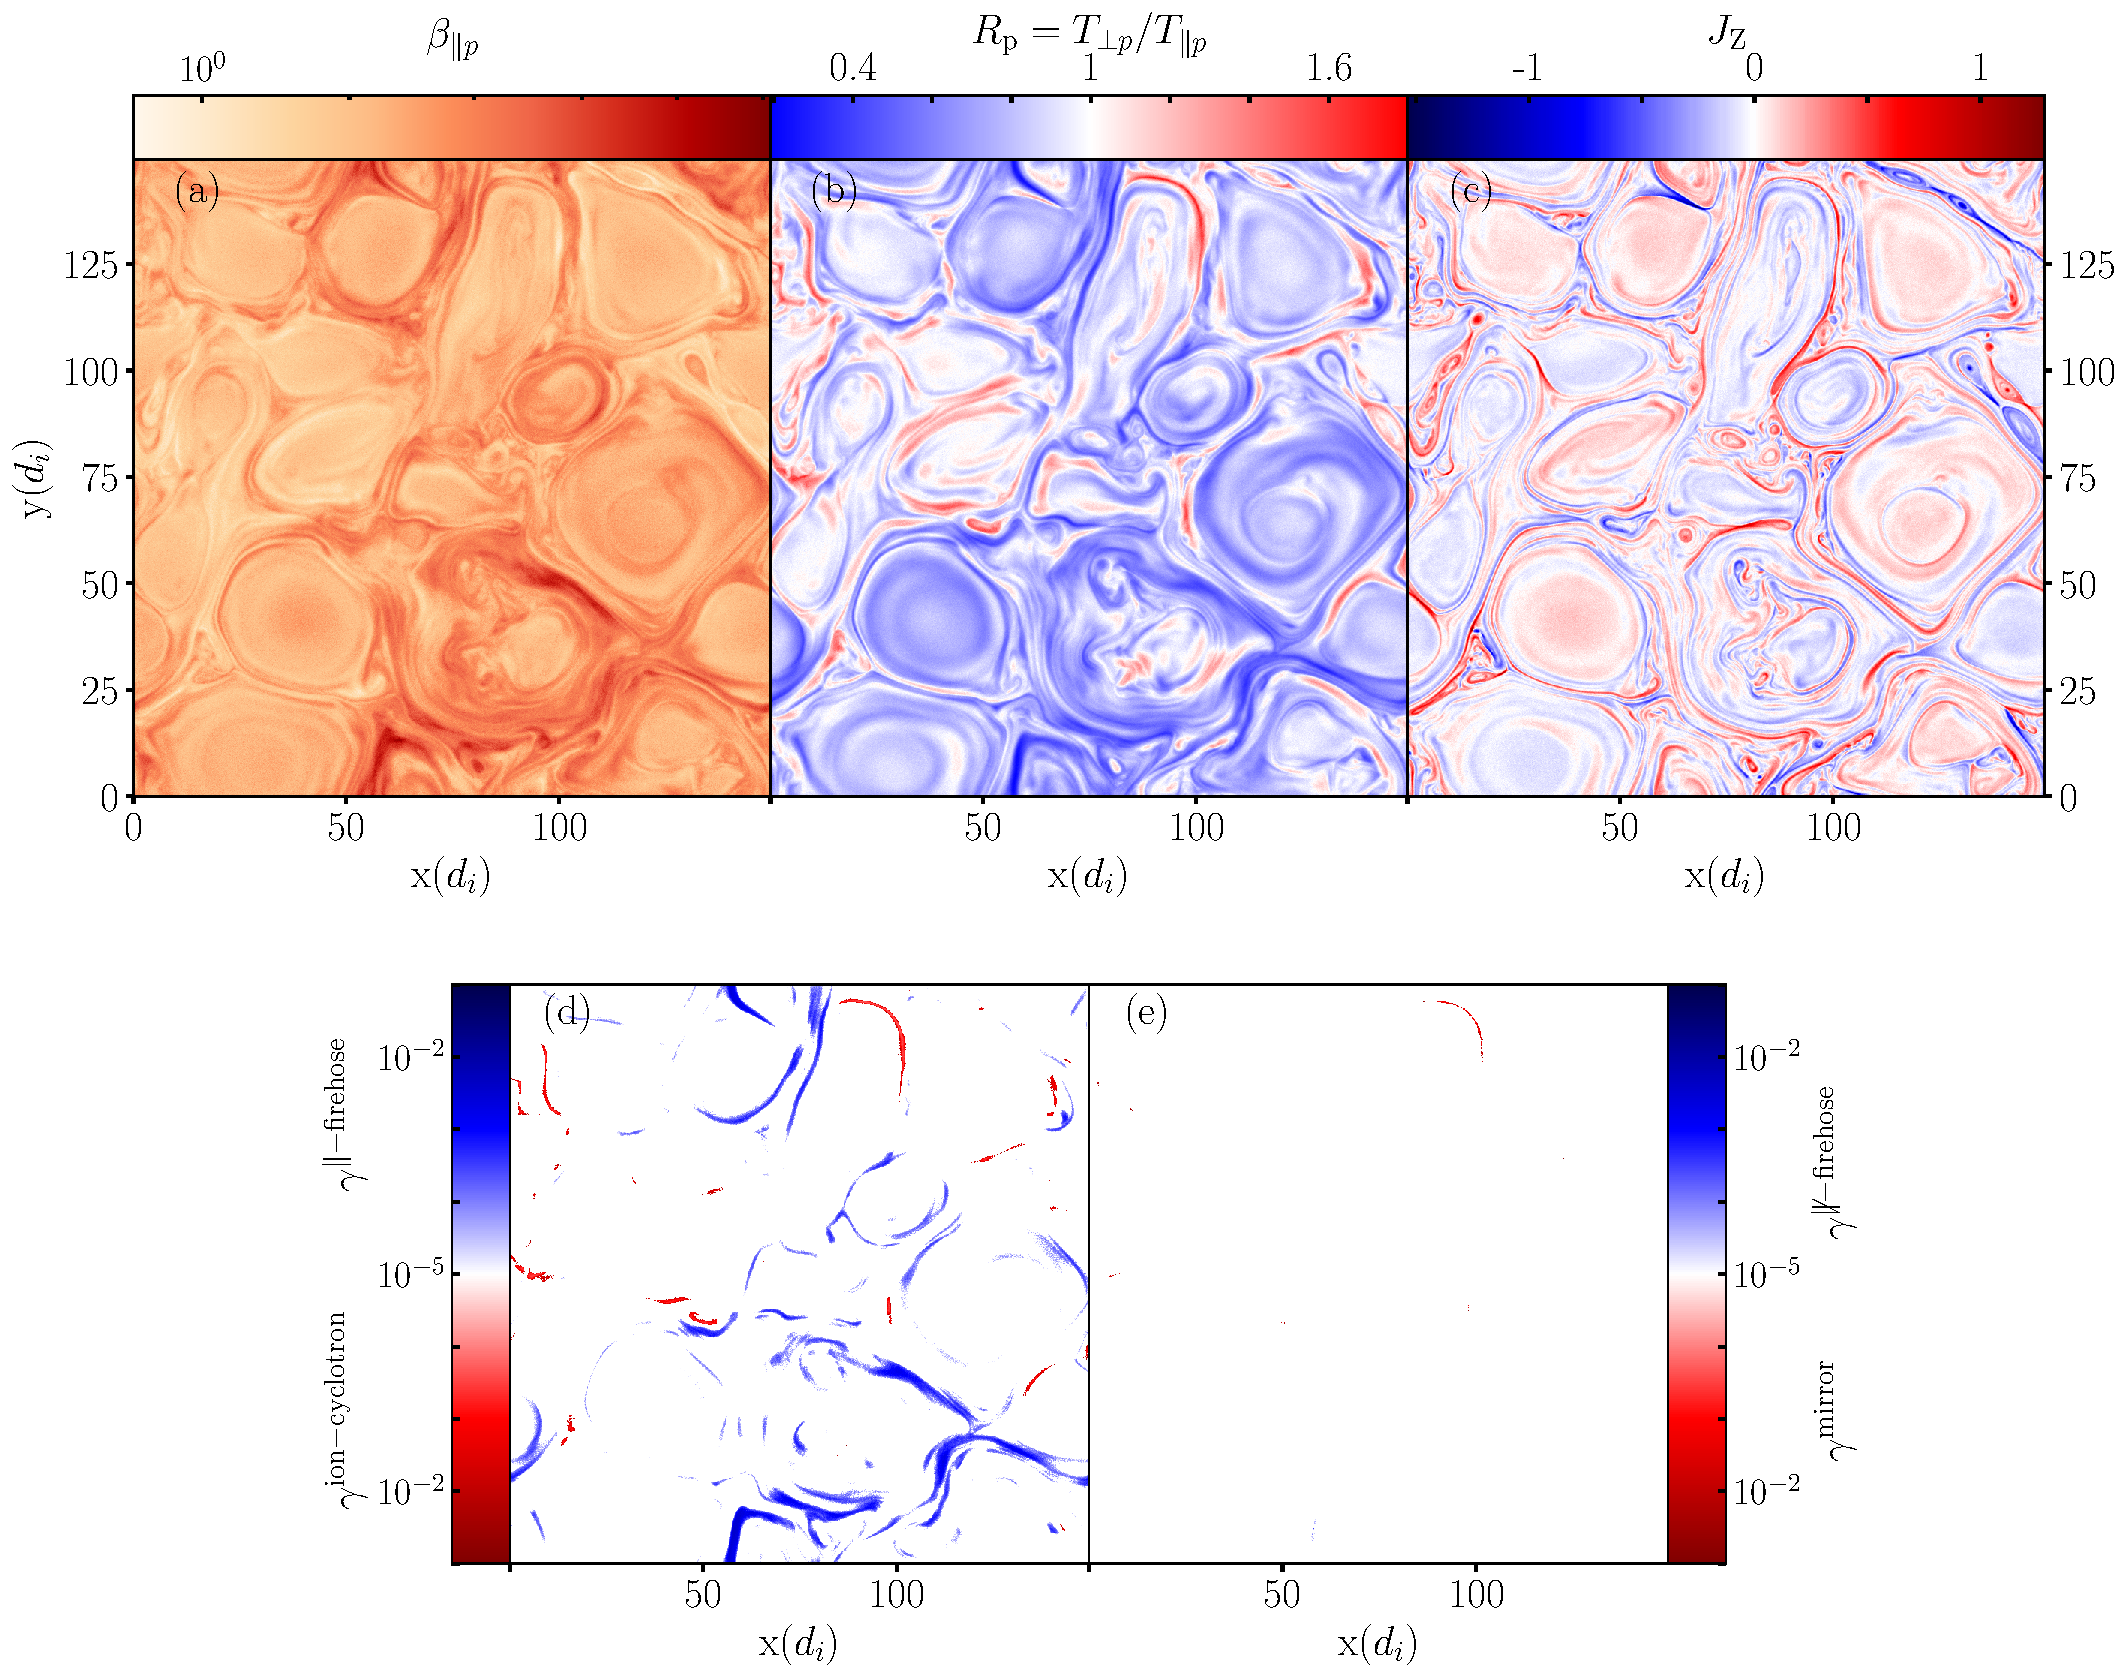
\includegraphics[width=1\textwidth]{figures/chap5/data_Rp_betap_jz_b_149p6_hb_gamma_k_149p6_hb.pdf}
                    \caption[Plot of $\beta_{\parallel \rm p}, R_{\rm p}, J_{\rm z} \mathrm{\,and\,}
                    \gamma$ for \texttt{149p6} dataset]{Colorplot of (top row, left to right)
                    $\beta_{\parallel \rm p}, R_{\rm p} \mathrm{\,and\,} J_{\rm z}$ for
                    \texttt{149p6} dataset. Panel (d) and (e) (bottom row) show the spatial
                    distribution of $\gamma_{\max}$ for parallel and oblique propagation
                    respectively corresponding to first two panels. \textit{Figure reproduced from
                    \citet{Qudsi2020a} with the permission of
                    \href{https://publishing.aip.org/}{AIP Publishing}} (see
                    \Cref{apdx:D}).}
                    \label{fig:brjhb}
                \end{center}
            \end{figure}

            \begin{figure}
                \begin{center}
                    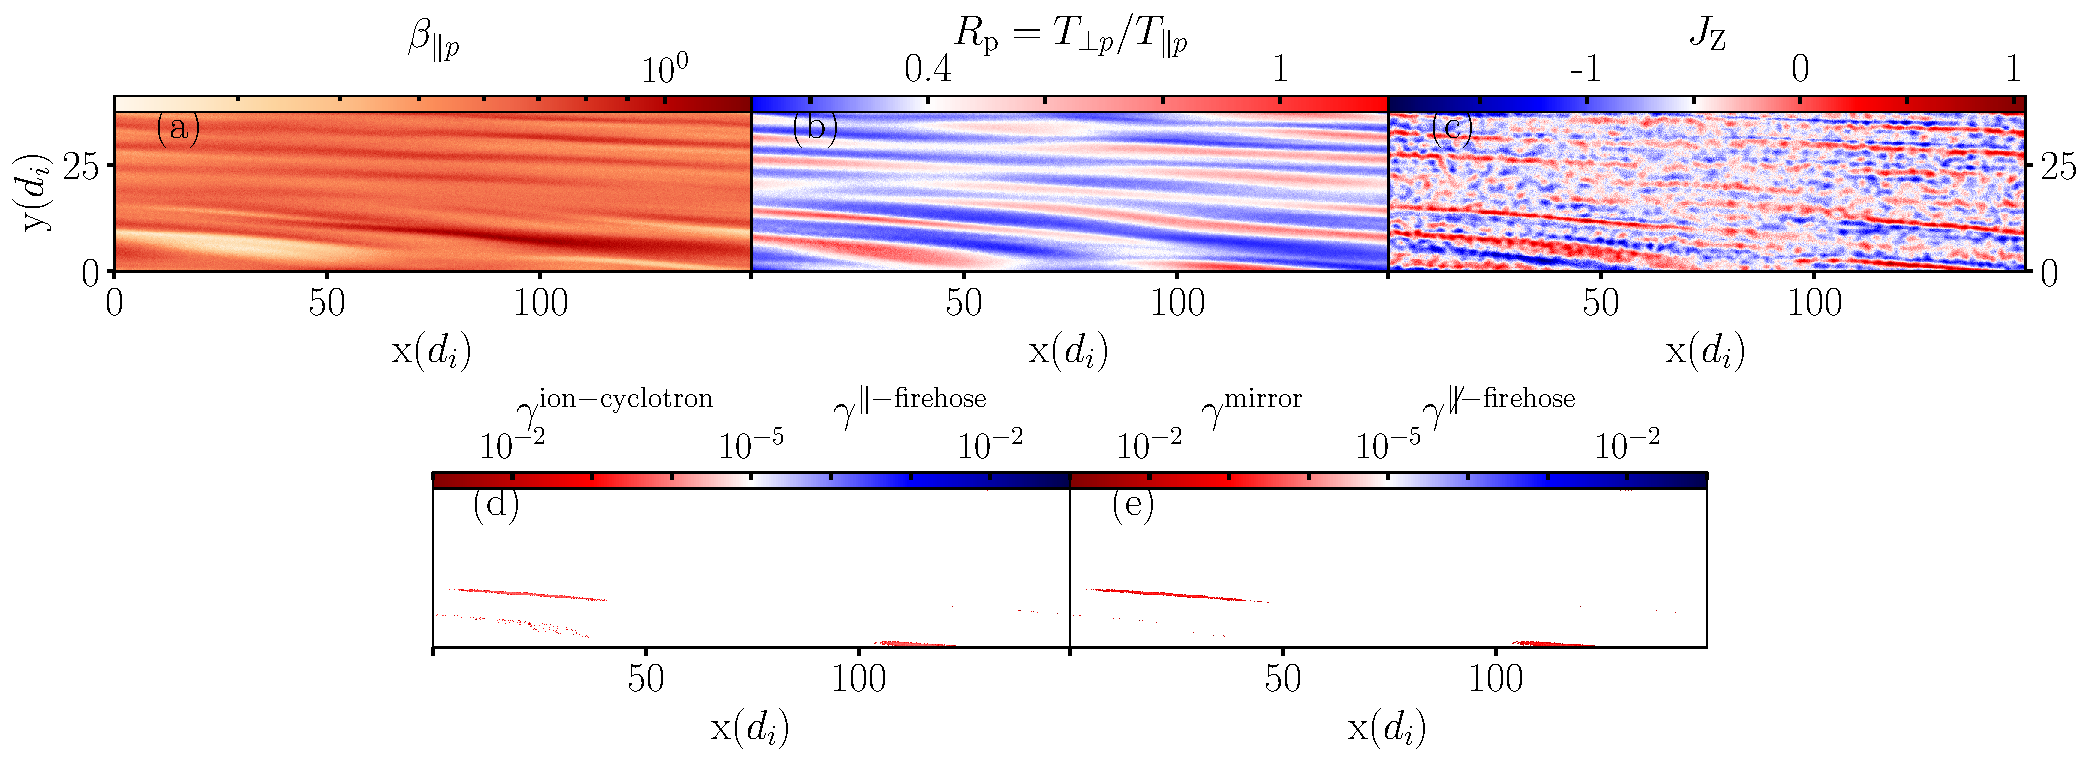
\includegraphics[width=1\textwidth]{figures/chap5/data_Rp_betap_jz_b_kaw_ti0p6te0p6_Time6000wpe_gamma_k_kaw_ti0p6te0p6_Time6000wpe.pdf}
                    \caption[Plot of $\beta_{\parallel \rm p}, R_{\rm p}, J_{\rm z} \mathrm{\,and\,}
                    \gamma$ for \texttt{kaw} dataset]{Colorplot of (top row, left to right)
                    $\beta_{\parallel \rm p}, R_{\rm p} \mathrm{\,and\,} J_{\rm z}$ for \texttt{kaw}
                    dataset. Panel (d) and (e) (bottom row) show the spatial distribution of
                    $\gamma_{\max}$ for parallel and oblique propagation respectively corresponding
                    to first two panels.}
                    \label{fig:brjkaw}
                \end{center}
            \end{figure}

            \begin{figure}
                \begin{center}
                    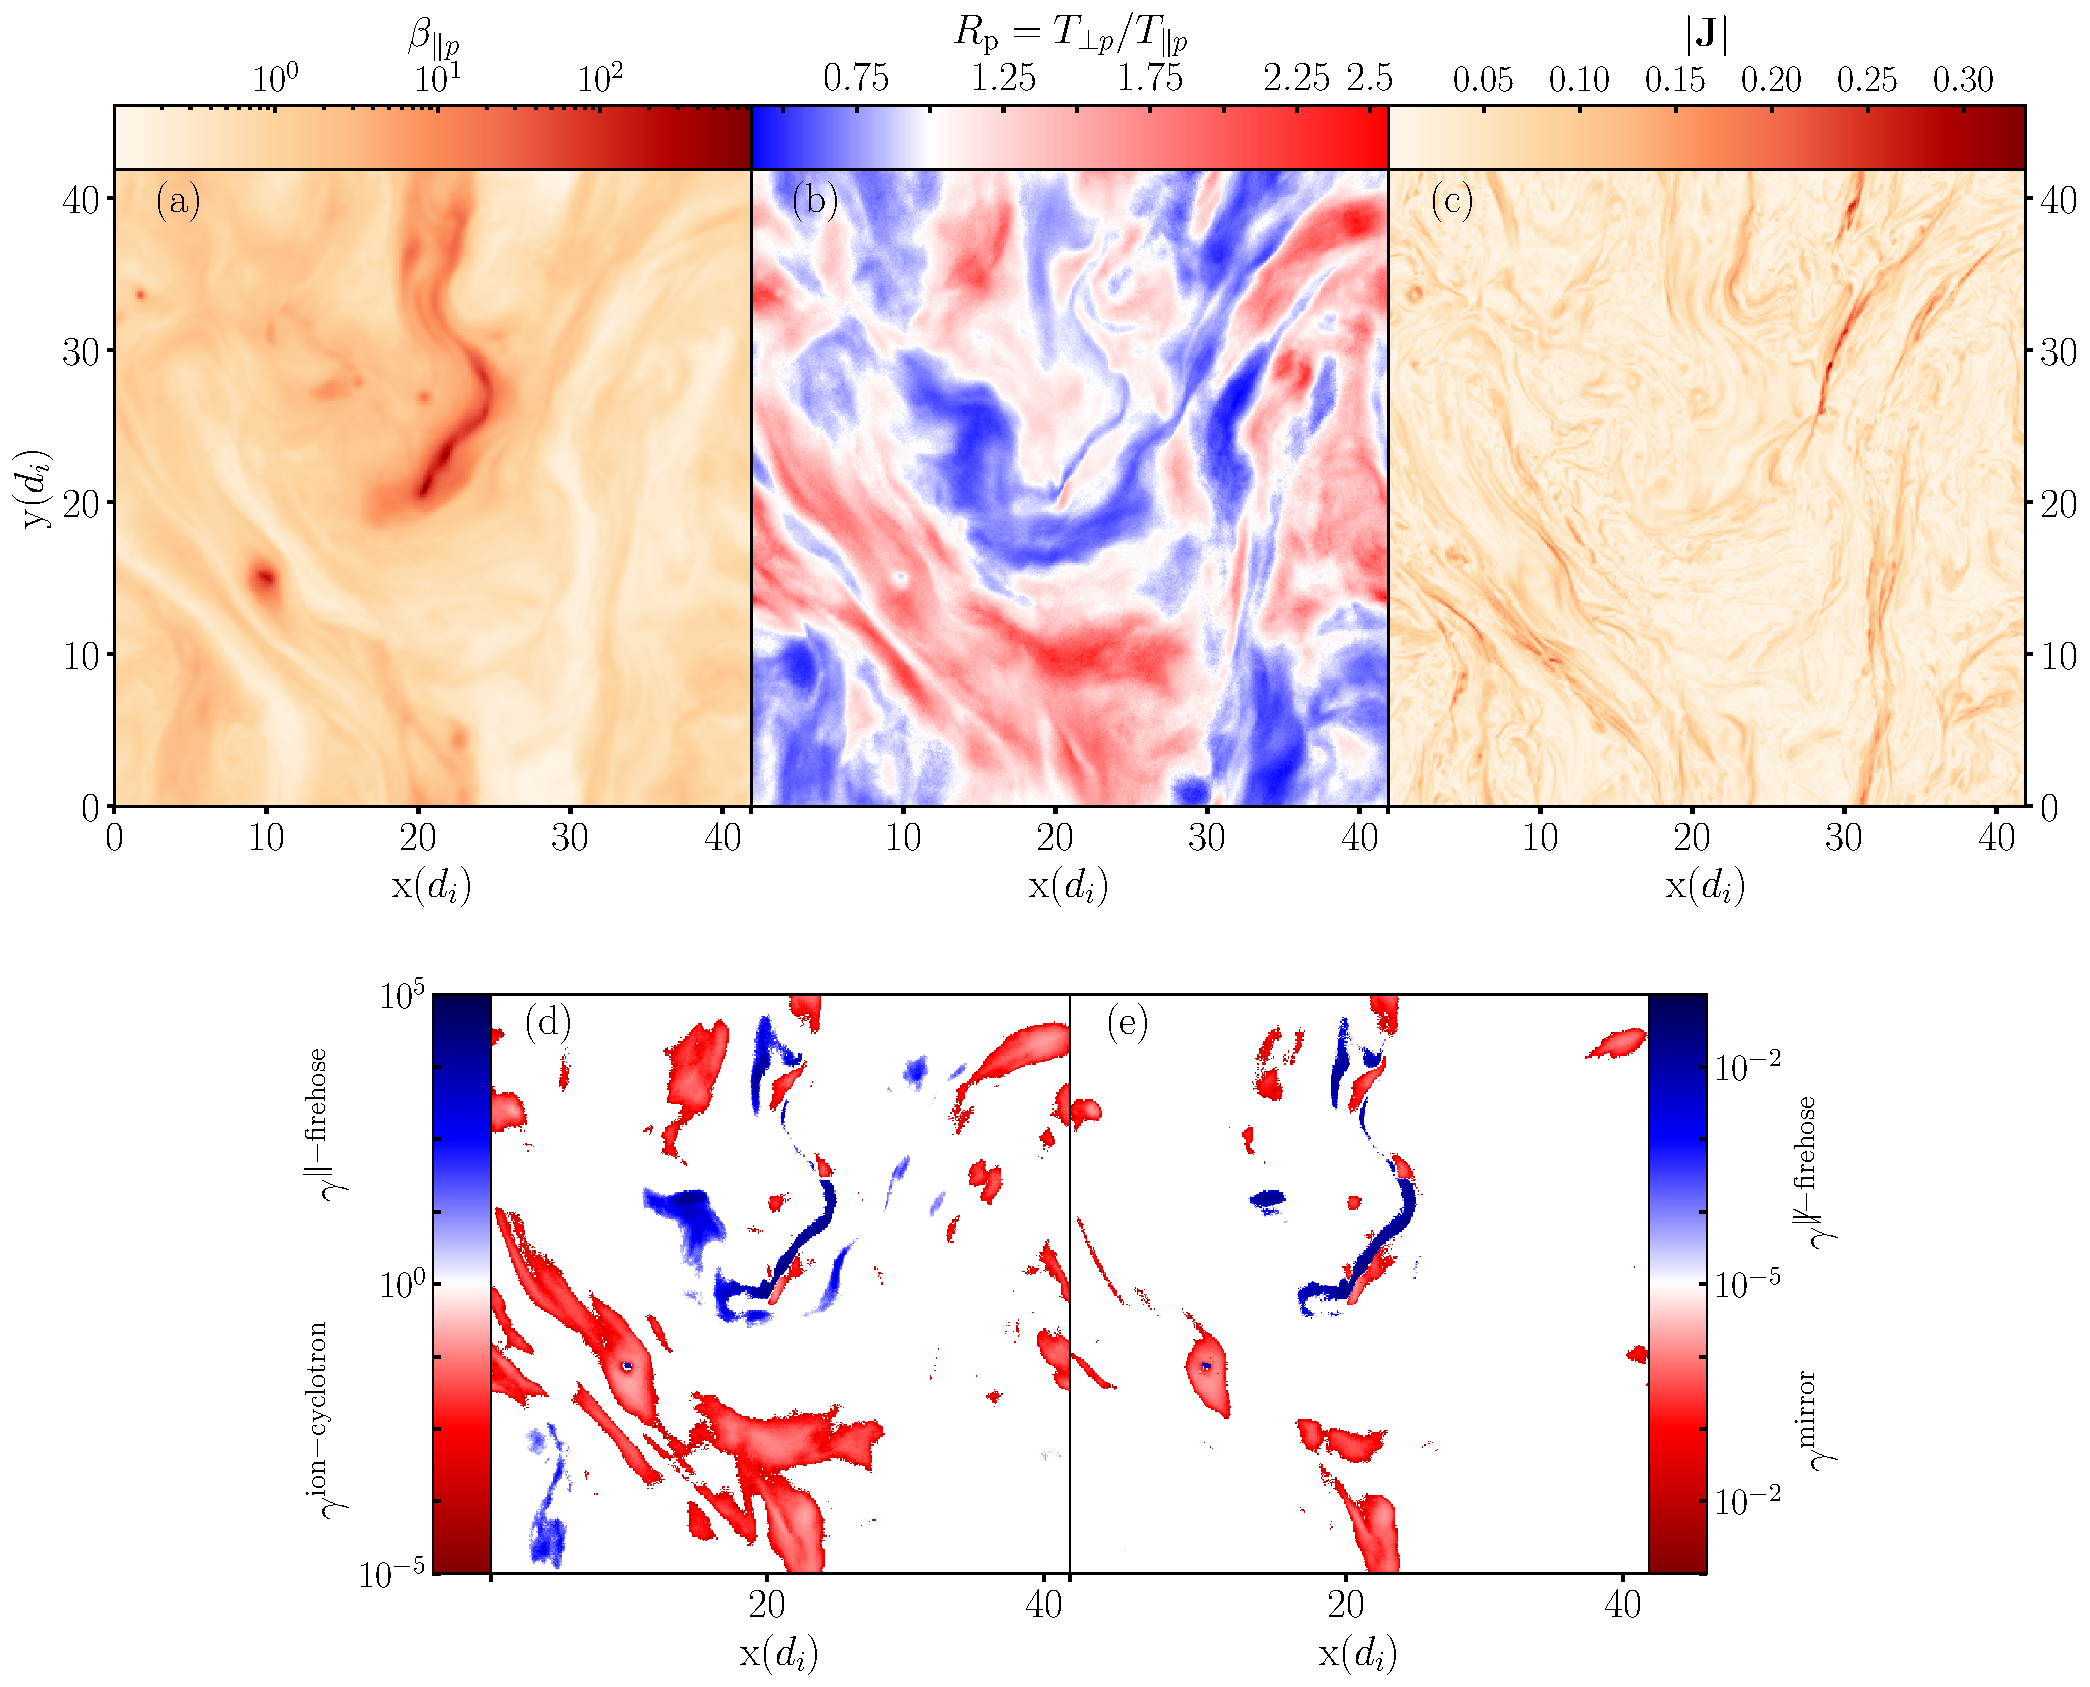
\includegraphics[width=1\textwidth]{figures/chap5/3Ddata_Rp_betap_b_yan512_gamma_k_yan_512.pdf}
                    \caption[Plot of $\beta_{\parallel \rm p}, R_{\rm p}, J_{\rm z} \mathrm{\,and\,}
                    \gamma$ for \texttt{ros} dataset]{Colorplot of (top row, left to right)
                    $\beta_{\parallel \rm p}, R_{\rm p} \mathrm{\,and\,} J_{\rm z}$ for \texttt{ros}
                    dataset. Panel (d) and (e) (bottom row) show the spatial distribution of
                    $\gamma_{\max}$ for parallel and oblique propagation respectively corresponding
                    to first two panels.}
                    \label{fig:brjros}
                \end{center}
            \end{figure}

            Using the method described in \Cref{sec:cgr,chap:chap4}, we computed
            $\gamma_\mathrm{\max}$ for the $(\beta_{\parallel \rm p},R_{\rm p})$-pair at each grid
            point of the simulation box, where $\gamma_\mathrm{\max}$ is the maximum value of growth
            rate for all possible values of propagation vector (\textbf{k}). The fourth and fifth
            Panels (d) and (e) of \Crefrange{fig:brjhb}{fig:brjros} show the spatial distribution of
            growth rates for the solutions with positive growth rates, corresponding to the first
            two panels of the same figure. As described in \Cref{sec:cgr}, for
            $\gamma_\mathrm{max}$, we imposed a cut-off at $10^{-5}\,\Omega_{\rm p}$; thus growth
            rates less than $10^{-5}\,\Omega_{\rm p}$ are considered to be 0. The Panel (d) of each
            figure (\Crefrange{fig:brjhb}{fig:brjros}) corresponds to the parallel modes (cyclotron
            for $R_{\rm p} > \,1$ and parallel firehose for $R_{\rm p} < \,1$), whereas the Panel
            (e) are for the oblique propagation (mirror for $R_{\rm p} > \,1$ and oblique firehose
            for $R_{\rm p} < \,1$). The paucity of blue color in the fifth panel of
            \Cref{fig:brjhb,fig:brjkaw} implies that the $\beta_{\parallel \rm p}$ (and/or $R_{\rm
            p}$) was rarely high (low) enough to excite any mode of oblique firehose instability.

            Comparing Panel (b) to Panel (d) and (e) of these figures, we see that values of
            $\gamma_\mathrm{max}>0$ are concentrated in distinct, thin regions of the $xy$-plane
            where extreme values of temperature anisotropy also occur. We also note that, for
            \Cref{fig:brjhb} because the simulation is 2.5D with $\mathbf{B_{\rm 0}}$ perpendicular
            to the simulation plane, the growth of instabilities such as the proton cyclotron and
            the parallel proton firehose with maximum growth at $\mathbf{k \times B_{\rm 0} = 0}$ is
            suppressed. However, for the other two simulations (\Cref{fig:brjkaw,fig:brjros}) that
            is not the case. Consequently, we see a lot of parallel instability in \Cref{fig:brjros}
            and a much higher value of average growth rate for \texttt{kaw} and \texttt{ros}
            datasets compared to \texttt{149p6} (see \Cref{fig:ratio_kde_all} and associated
            discussion). However, despite not being suppressed in the parallel direction, parallel
            instabilities in \Cref{fig:brjkaw} remain relatively sparse because of very low value of
            $\beta_{\parallel \rm p}$ (see \Cref{tab:datadetail4a}). Comparatively \Cref{fig:brjros}
            shows much less sparsity as a consequence of high value of $R_{\rm p}$ over an extended
            region of the simulation box.

        \subsection{Spacecraft Observations} \label{sec:spcr5}

            \begin{sidewaysfigure}
                \begin{center}
                    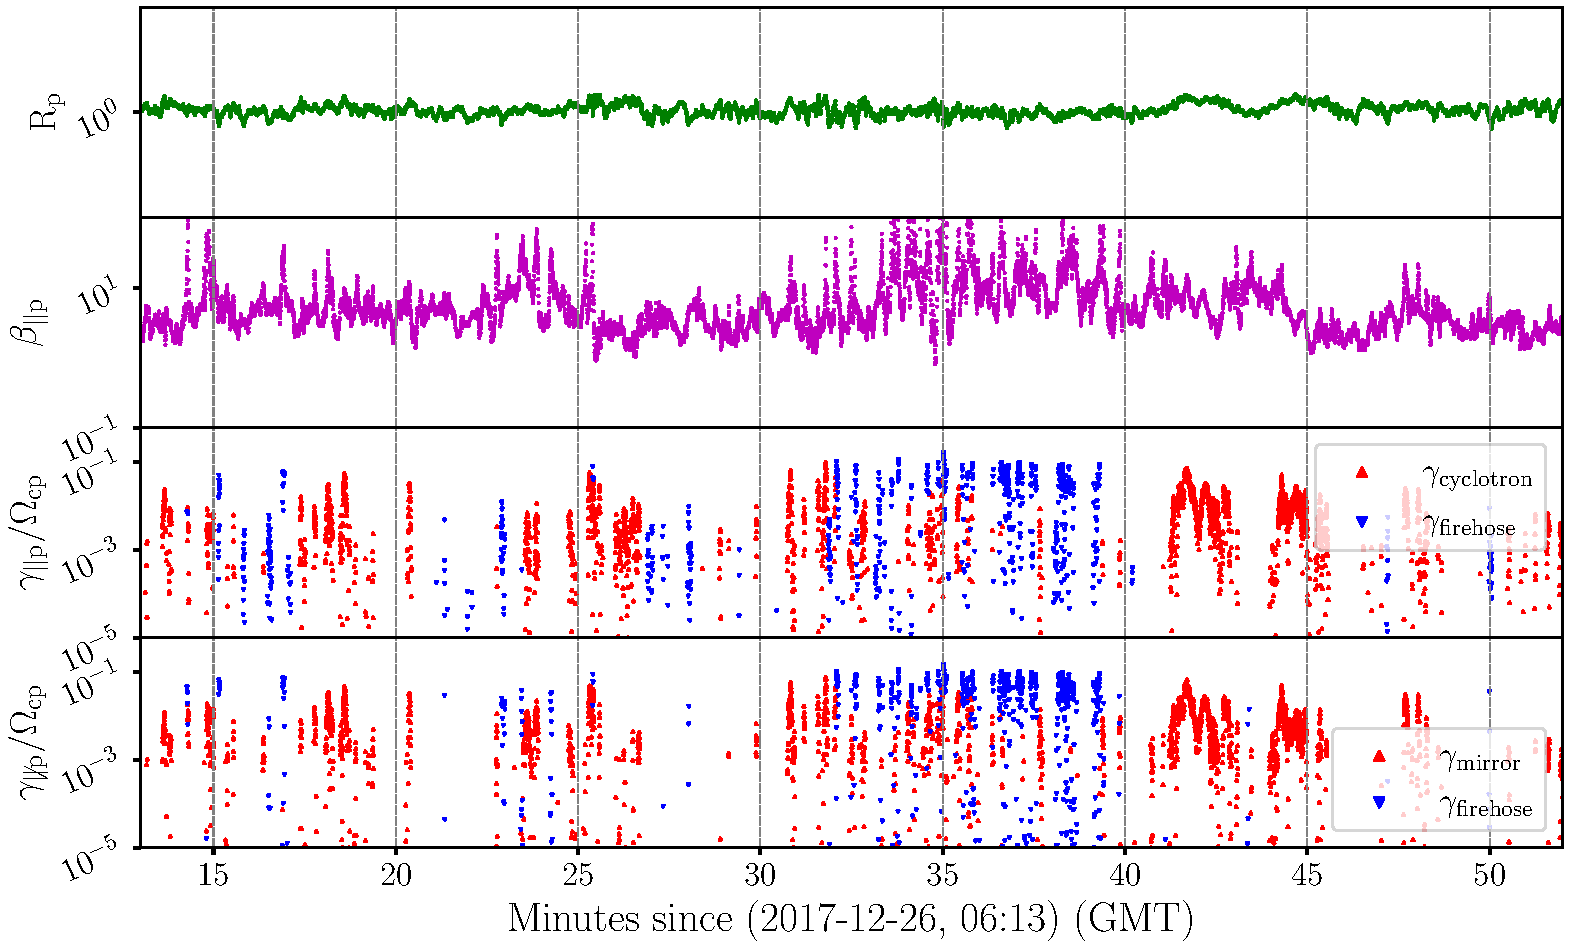
\includegraphics[width=1.\textwidth]{figures/chap5/mms_all_piecewise_2017-12-26_2017-12-26_00000108_00015707.pdf}
                    \caption[Time series plot of $\beta_{\parallel \rm p}, R_{\rm p}, J_z
                             \mathrm{\,and\,} \gamma$ for \texttt{mms} dataset]{Time series plot of
                             proton anisotropy ratio $(R_{\rm p})$, proton parallel beta
                             $(\beta_{\parallel \rm p})$, total current density in
                             $\mathrm{nA/m^2}$, parallel instability growth rates (proton-cyclotron,
                             in red and parallel firehose in blue), and oblique instability growth
                             rates (mirror in red and oblique firehose in blue), as observed by MMS
                             on 2017 December 26.}
                    \label{fig:brjmms}
                \end{center}
            \end{sidewaysfigure}

            \begin{sidewaysfigure}
                \begin{center}
                    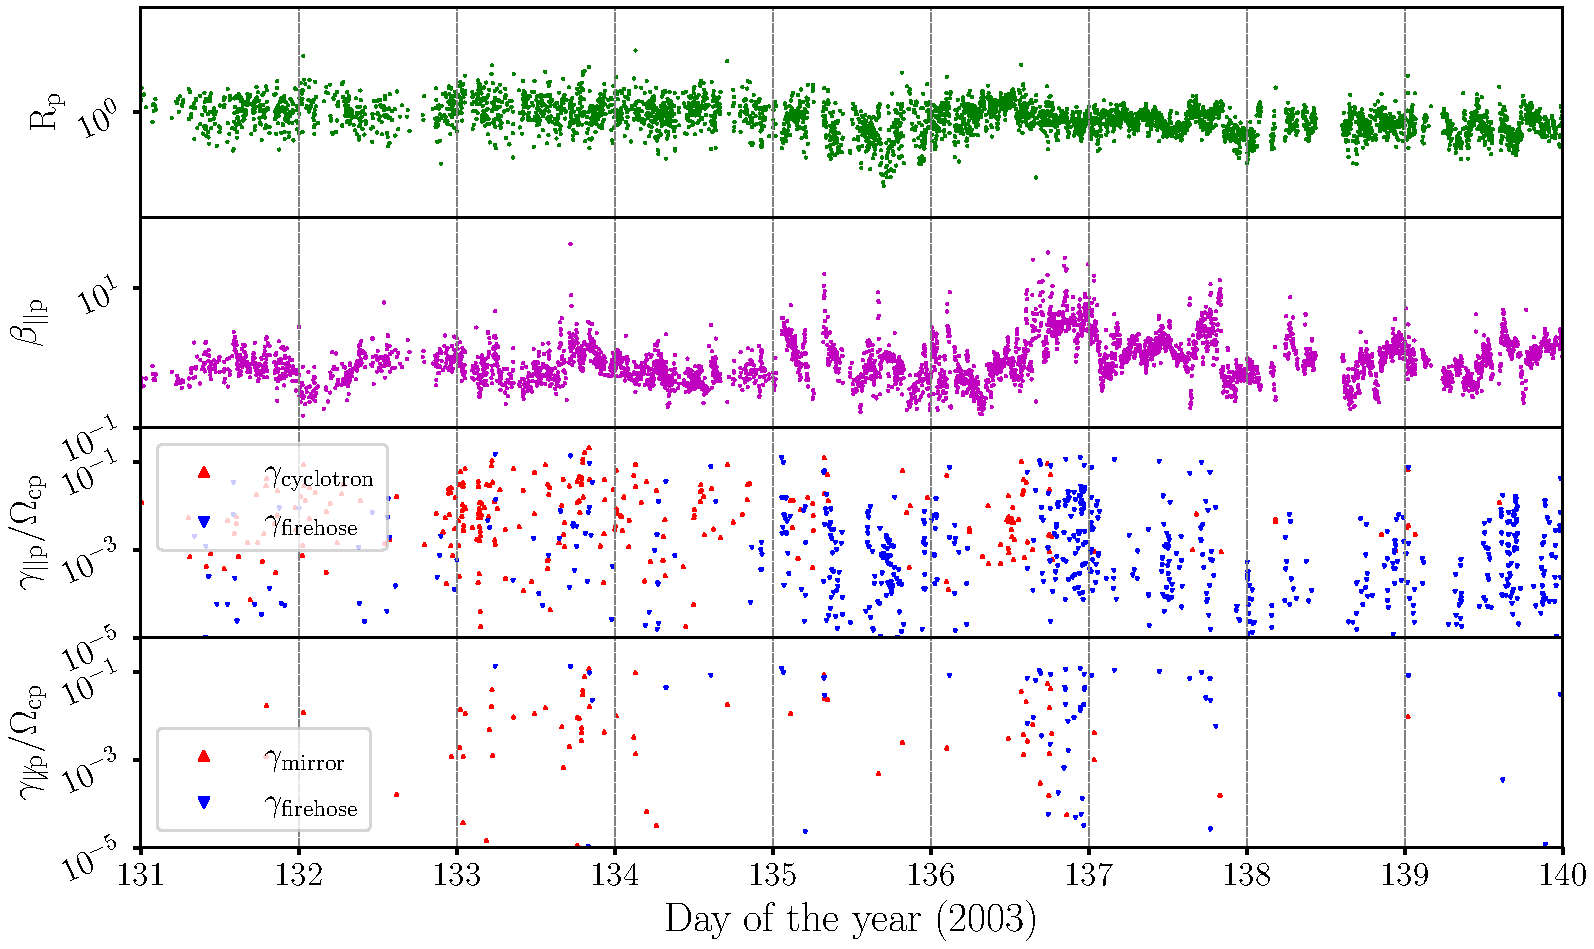
\includegraphics[width=1.\textwidth]{figures/chap5/wind_all_piecewise_2003-5-11_2003-5-19_01207878_01212368.pdf}
                    \caption[Time series plot of $\beta_{\parallel \rm p}, R_{\rm p}, J_{\rm z}
                             \mathrm{\,and\,} \gamma$ for \texttt{wnd} dataset]{Time series plot of
                             proton anisotropy ratio $(R_{\rm p})$, proton parallel beta
                             $(\beta_{\parallel \rm p})$, parallel instability growth rates
                             (proton-cyclotron, in red and parallel firehose in blue), and oblique
                             instability growth rates (mirror in red and oblique firehose in blue),
                             as observed by Wind.}
                    \label{fig:brjwnd}
                \end{center}
            \end{sidewaysfigure}

            \begin{figure}
                \begin{center}
                    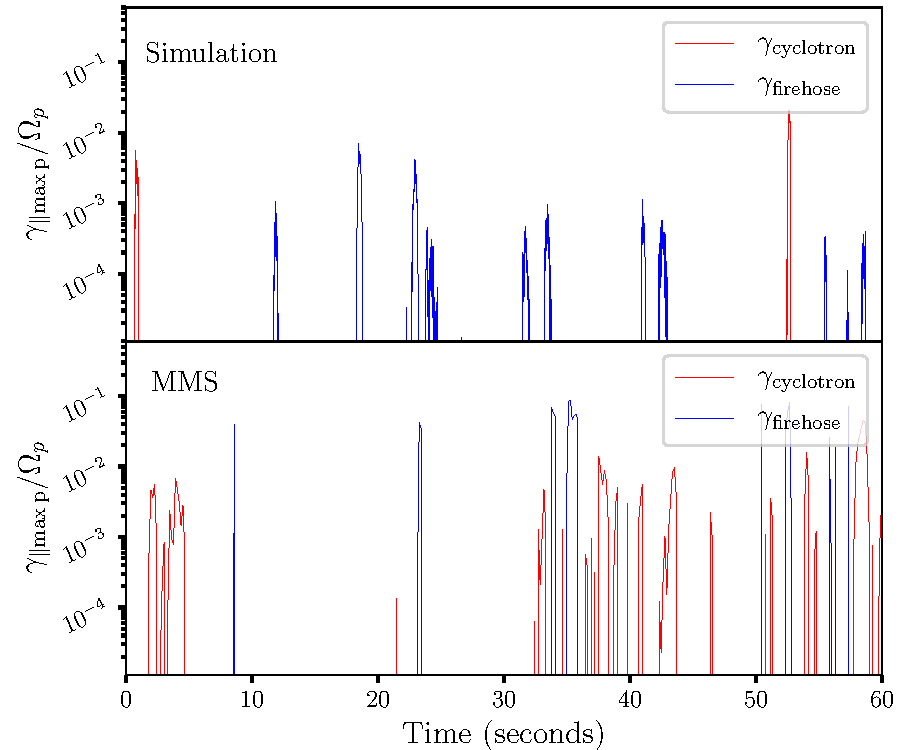
\includegraphics[width=1.\textwidth]{figures/chap5/SpaceCraft_simulation_mms.pdf}
                    \caption[Spacecraft and simulation comparison of $\gamma$ time
                            series]{Comparison of simulation and MMS time series for
                            $\gamma_{\parallel max}$ values for a 1-minute period. The top panel
                            shows the distribution for a 1-minute long flight through the simulation
                            box and the lower panel shows the distribution of $\gamma_\mathrm{max}$
                            starting at 06:34 on 2017 December 26. \textit{Figure reproduced from
                            \citet{Qudsi2020a} with the permission of
                            \href{https://publishing.aip.org/}{AIP Publishing}} (see
                            \Cref{apdx:D}).}
                    \label{fig:spcsim}
                \end{center}
            \end{figure}

            \Cref{fig:brjmms} and \Cref{fig:brjwnd} show a typical portion of the time series data
            from two spacecraft: MMS and Wind. The panels, from top to bottom show $R_{\rm p},
            \beta_{\parallel \rm p}, |\mathbf{J}|$ and maximum growth rates ($\gamma_\mathrm{max}$)
            for parallel and oblique instabilities respectively for both the spacecraft. Time
            intervals were chosen so that the figures showed approximately equal numbers of
            correlation time scales in the magnetosheath and solar wind at 1\,au. For magnetosheath
            10 minute corresponds to roughly 20 $\tau_{\rm cr}$ \citep{Le1993,Gutynska2008} whereas
            for solar wind which has a correlation time length of about 55 minutes the interval of
            24 hours corresponds to about 25 times $\tau_{\rm cr}$ \citep{Matthaeus1982,Wicks2010}.

            Both the \Cref{fig:brjmms,fig:brjwnd} show an intermittent distribution of instability
            growth rates, though in case of Wind since the variation in $\beta_{\parallel \rm p}$ is
            much smaller than that observed in magnetosheath the number of unstable points are
            significantly smaller. \Cref{tab:datadetail4a} lists out the variation in these
            parameters for all the different cases discussed so far.

            \begin{table}[ht]
                \centering
                \caption[Average value of parameters for datasets]{Average values of parameters for
                different datasets}
                \begin{tabular}{ p{0.1\linewidth} p{0.30\linewidth} p{0.1\linewidth}
                p{0.1\linewidth} p{0.12\linewidth}}
                    \hline
                    \\
                    Name & Type of data & $\left<\beta_{\parallel \rm p}\right>$ & $\left<R_{\rm
                    p}\right>$ & $n_\gamma/N$ (\%)\\
                    \\
                    \hline
                    \\
                    \texttt{149p6} & Simulation & 0.64 & 0.83 & 6.82 \\
                    \\
                    \hline
                    \\
                    \texttt{kaw} & Simulation & 0.61 & 0.89 & 0.90 \\
                    \\
                    \hline
                    \\
                    \texttt{ros} & Simulation & 0.84 & 1.04 & 16.39 \\
                    \\
                    \hline
                    \\
                    \texttt{mms} & Spacecraft \newline Observation\newline (Magnetosheath) & 4.29 &
                    1.04 & 24.51 \\
                    \\
                    \hline
                    \\
                    \texttt{wnd} & Spacecraft \newline Observation\newline (Solar Wind) & 0.69 &
                    0.50 & 14.22 \\
                    \\
                    \hline
                \end{tabular}
                \label{tab:datadetail4a}
            \end{table}

            Comparing \Cref{fig:brjhb} and \Cref{fig:brjmms} we see that a larger fraction the MMS
            data ($30\%$) are unstable versus grid points from the simulation ($0.8\%$), with
            $\gamma_\mathrm{max}$ values above the cut-off ($10^{-5}\,\Omega_{\rm p}$). This
            discrepancy arises in part because MMS data have much higher values of $\beta_{\parallel
            \rm p}$ than the simulation (median values of 4.5 and 1.2, respectively). Furthermore,
            \citet{Servidio2015} found that, for a given value of $\beta_{\parallel \rm p}$,
            simulations of the turbulence type, like in the present 2.5D cases, generally admit less
            extreme temperature-anisotropy than are seen in space observations, because typical
            simulations are of modest size resulting in modest Reynolds number and lack large scale
            coherent driving.

            The time series for MMS observation (\Cref{fig:brjmms}) exhibits intermittent structure
            in the distribution of growth rates that are similar to what we see in Panels (d) and
            (e) of \Cref{fig:brjhb} for simulation. \Cref{fig:spcsim}, which shows the comparison of
            the time series of simulation and MMS data for a 1\,minute period, shows that
            qualitatively they have similar distribution. Time series for the simulation was
            computed by flying a virtual spacecraft, travelling at the plasma bulk speed (238\,km/s,
            same speed as that of plasma during MMS observation), through the entire box at an angle
            of 75 degrees with respect to $x$-direction.

            In \Cref{fig:brjmms} the points of instabilities ($\gamma_\mathrm{max}>0$) are
            concentrated together, spreading over a small time interval lasting typically a few
            seconds (4-8\,seconds) with sharp peaks. Though in this study we did not quantify the
            length scale of all the peaks, we found that typically they are spread over a length
            scale of $\sim 20-40\,\mathrm{d_{\rm i}}$, where $\mathrm{d_{\rm i}}$ is the
            ion-inertial length and the length scale was calculated using the flow speed of the
            plasma and the duration of the peak.

    \section{Discussions} \label{sec:conc5}

        In recent years, two different perspectives have been widely used to explain the behavior of
        the solar wind, magnetosheath, and similar space plasmas. In the first picture, the linear
        theory of plasma instability, at high $\beta_{\parallel \rm p}$, for extreme $R_{\rm p}$,
        different instability thresholds become active, thereby confining the plasma population to
        lower values of $R_{\rm p}$
        \citep{Gary2001,Kasper2002,Hellinger2006,Matteini2007,Klein2018}. In the second, turbulence
        generates sharp gradients in the plasma that produce temperature anisotropy
        \citep{Osman2011,Greco2012,Valentini2014,Parashar2016}.

        These two theories have been non-reconcilable because of the basic underlying assumption.
        The linear theory of plasma instability assumes a homogeneous background magnetic field
        whereas turbulence relies on large fluctuations in the field. It was hitherto unclear if
        these two seemingly disparate processes--microinstabilities and turbulence\index{turbulence}--are connected in
        any way in configuration space. The apparent contradiction---homogeneity against
        intermittent inhomogeneity---between the two interpretations poses a question of fundamental
        importance in the study of space plasmas specifically and collisionless plasmas in general:
        How can an inhomogeneous phenomenon such as turbulence be consistent with
        temperature-anisotropy constraints derived from linear theory of homogeneous plasmas? Our
        simulations show that the turbulence indeed heats the plasma anisotropically, making it more
        susceptible to instability. But the simulation also show that these anisotropies are
        strongly localized; furthermore the 2.5-D character of the simulation with a strong
        background magnetic field out of the simulation plane acts against the growth of the proton
        cyclotron and parallel proton firehose microinstabilities. Clearly, further studies are
        necessary to resolve this apparent contradiction.

        Although there is no discussion of the consequences of electron anisotropies here, it should
        be noted that both simulations and magnetosheath observations \citep{Gary2005} have shown
        that electron temperature anisotropies in collisionless plasmas can drive whistler
        instabilities which, in turn, scatter the electrons to establish a constraint on the
        anisotropy of that species \citep{Gary1996}, in full analogy with the case of ion
        instabilities and anisotropy constraints discussed here.

        In \Crefrange{fig:brjhb}{fig:brjros} the regions of significant growth rates are close to
        the regions of peak current values. This suggests that current sheets are producing the
        extreme temperature-ansiotropies that ultimately drive the instabilities. Note, though, that
        the high-$\gamma_{\max}$ regions and the high-$J_{\rm z}$ regions do not perfectly overlap:
        they tend to be adjacent to each other rather than co-located, as seen by \citet{Greco2012}.
        Thus, traditional methods of correlation calculation would be inadequate to quantify the
        relationship between these two structures. Instead, an analysis using cross correlations of
        these quantities \citep[see, e.g.,][]{Parashar2016} or joint distributions \citep[see,
        e.g.,][]{Yang2017} to explore the causal connection between instabilities and
        turbulence-generated current sheets would be the next step forward.

        In this study we found an explicit connection between intermittency in plasma turbulence and
        indication of the local enhancement of linear instability growth rates. Intermittency is
        clearly influential in the interpretation of observations, while its theoretical importance
        derives from its potential connection to the nature and statistics of dissipation
        \citet{Kolmogorov1962, Karimabadi2013, Wan2016, Howes2015, Matthaeus2015}. The connection we
        have found here---that linear instability growth rates computed from (admittedly
        oversimplified) homogeneous plasma theory, also occur in intermittent bursts---adds to this
        emerging understanding of plasma dissipation. Previous studies found that pathways, such as
        inertial range transfer \citep{SorrisoValvo2019}, electromagnetic work \citep{Wan2012},
        electron energization \citep{Karimabadi2013}, and pressure-strain interactions
        \citep{Yang2017} concentrate in small sub-volumes of plasma turbulence. Dynamical processes
        that lead to dissipation such as magnetic reconnection, also occur in spatially localized
        regions \citep{Drake2008}. Along with these we now have observed strong indication that
        velocity-space driven phenomena \citep{Servidio2012a, Greco2012, Schekochihin2016,
        Servidio2015} also occur in similar highly localized sub-volumes. Observation and study of
        wave signatures which propagate in both directions and thus implying proximity to the
        generation region may provide a more conclusive evidence. The nature of the spatial or
        regional correlations of these kinetic processes to the surrounding dynamical processes that
        drive them largely remains to be explored.    % This file (chap5.tex) contains the text
                   % for Chapter 5.

\newpage\null\thispagestyle{empty}

%
% This is Chapter 6 file (chap6.tex)
%
\chapter{Temperature Enhancement Along Intermittent Structures}\label{chap:chap6}

    \section{Overview} \label{sec:ovrvw6}

        The solar wind proton temperature at 1\,au has been found to be correlated with small-scale
        intermittent magnetic structures, i.e., regions with enhanced temperature are associated
        with coherent structures such as current sheets. Using Parker Solar Probe data from the
        first encounter, we study this association using measurements of radial proton temperature,
        employing the Partial Variance of Increments (PVI)\index{PVI} technique to identify intermittent
        magnetic structures. We observe that the probability density functions of high-PVI events
        have higher median temperatures than those with lower PVI, The regions in space where PVI
        peaks were also locations that had enhanced temperatures when compared with similar regions
        suggesting a heating mechanism in the young solar wind that is associated with intermittency
        developed by a nonlinear turbulent cascade in the immediate vicinity. We also look into
        magnetosheath ion temperature using MMS and report on the findings.\footnote{Part of this
        study was published in \citet{Qudsi2020}.}

    \section{Introduction} \label{sec:intr6}

        As discussed in \Cref{sec:plas2}, solar wind is a stream of charged and highly magnetized
        plasma streaming at supersonic speed originating from the Sun. Solar wind is primarily
        composed of ionized hydrogen \citep{Marsch1982a, Kasper2012} with varying amount of helium
        nucleus \citep{Maruc2012} and minor heavier ions.

        Despite decades of observation, the exact process that originally heats and accelerates
        solar wind plasma remain unknown, but several candidates have been proposed. Turbulence
        cascade transfers energy from large to small scales (see \Cref{sec:inter3b} for more
        details), which can ultimately lead to dissipation and heating \citep{Velli1989, Velli1993,
        Matthaeus1999, Dmitruk2002, Cranmer2005, Cranmer2007, Cranmer2012, Cranmer2014, Verdini2007,
        Verdini2009, Verdini2009a, Chandran2009, Perez2013, Lionello2014}. Current sheets, generated
        by cascading vortices, can also lead to localized heating \citep{Parashar2009, Osman2011,
        Osman2012, Osman2012a, Gingell2015}. Wave particle interactions --- including, e.g.,
        microinstabilities, Landau damping, and ion-cyclotron resonance --- can likewise result in
        significant changes to the particles' phase-space distribution \citep{Gary1993,
        Sahraoui2010, Klein2015}. Though there are several linear and non-linear mechanisms which
        heats the space plasma, here we focused on one such mechanism, coherent structures: features
        in the plasma that are persistent through time, concentrated in space, or both
        \citep{Greco2018}. As discussed in \Cref{sec:intmt} such structures can be produced by
        turbulent cascade \citep{Osman2012a} and are also associated with current sheets
        \citep{Yordanova2016}. \citet{Osman2011, Osman2012a} analyzed in-situ observations and of
        near-Earth solar wind and found clear indications that coherent structures correlate with
        local enhancements in temperature.

        So far most of the studies have been done using either numerical simulation data or solar
        wind data at 1\,au. However, plasma conditions are a lot different at 1\,au from those very
        close to the Sun, say 0.2\,au. Magnetic field near 0.2\,au is $\sim$\,70\,nT compared to
        $\sim$\,5\,nT at 1\,au. Plasma at 0.2\,au is also much denser and hotter ($\sim$\,200\,
        /$\mathrm{cm^{-3}}$ and $\sim\,10^6$\,K compared to $\sim$\,5\,/$\mathrm{cm^{-3}}$ and
        $\sim\,10^4$\,K respectively) \citep{Kasper2019}. And even though solar wind is mostly
        collisionless, plasma at 1\,au has gone through more processing compared to the young solar
        wind \cite[\S3.3 \& references therein]{Verscharen2019}. The recently launched Parker Solar
        Probe (PSP) provides an unprecedented opportunity to study the nascent solar wind in great
        detail.

        In this study, we revisit the techniques of \citet{Osman2011, Osman2012a}, and, by applying
        them to observations from
        \discolorlinks{\href{https://www.nasa.gov/content/goddard/parker-solar-probe}{Parker Solar
        Probe}} (PSP), explore the relationship between plasma structures and heating in nascent
        solar wind plasma. We also look into the heating of terrestrial magnetosheath plasma using
        data from MMS. \Cref{sec:bgnd6} provides the background on such structures and introduces
        the reader to the physics of technique employed in data analysis which is described in
        \Cref{sec:data6}. In \Cref{sec:diss6} we present the results and discuss its implication.
        \Cref{sec:conc6} summarizes the results along with a conclusion and potential future works.

    \section{Background} \label{sec:bgnd6}

        Some recent studies, both observational and numerical, have shown that intermittent
        structures are correlated with the regions of enhanced temperature in the plasma
        \citep{Osman2012, Osman2011, Greco2012} and understanding the mechanisms by which the
        turbulence heats the plasma may also help solve the coronal heating problem
        \citep{Osman2012a}. This is a particularly attractive scenario especially given the ubiquity
        of the localized structures. Study performed on data from PIC simulation by \citet{Wu2013}
        shows that the correlation between enhanced temperature and coherent structures exists for
        sub ion inertial length ($d_{\rm i}$). Further evidence of this is provided by
        \citet{TenBarge2013} for Gyrokinetic simulation, \citet{Parashar2009, Wan2012,
        Karimabadi2013, Wan2015} for PIC and \citet{Servidio2012, Servidio2015} for Vlasov
        simulations respectively. Work done by \citet{Chasapis2015} and \citet{Yordanova2016} on
        from Cluster and MMS data show similar results from observation vantage point.

        In this study, we investigate these discontinuities in the magnetic field and explore their
        association with local enhancements in ion temperature. As discussed in \Cref{sec:intmt} we
        use PVI (see \Cref{eq:pvi} for the expression of PVI) to identify the discontinuities.
        Although these structures constitute only a small fraction of total data set their
        contribution to the total internal energy per unit volume is high. This emphasizes the
        importance of using the PVI technique for such studies. We also note that an analogous
        examination of the association of PVI events with energetic particles was carried out at
        1\,au, \citep{Tessein2016}.

    \section{Data Selection and Methodology} \label{sec:data6}

        We analyzed data from PSP's first encounter with the Sun (October 31 to November 11, 2018).
        The FIELDS fluxgate magnetometers provided measurements of the local magnetic field at a
        rate of 64\,samples/NYseconds. Radial proton temperature/thermal speed data was obtained
        from the Solar Probe Cup (SPC), part of the Solar Wind Electron, Alpha and Proton suite
        \citep{Kasper2016} (See \Cref{sec:psp} for a more detailed discussion of PSP, SPC, FIELDS
        and the dataset used in this study). The average speed of solar wind during the first
        encounter was around 350\,km/s for the most part and crossed 500\,km/s only on the last day
        of the encounter. Thus, using Taylor’s Hypothesis, 1\,NYs corresponds to a length scale of
        300\,km.

        For the calculation of PVI according to \Cref{eq:pvi}, we used 64\,NYHz data, with a lag of
        1\,NYs, which is the native cadence of SPC \citep{Kasper2016}. The ensemble averaging was
        done over 8\,hours, which is several times the estimated correlation time. In this study we
        used the correlation time computed in \citet{Parashar2020}. However there are few subtleties
        associated with this calculation, and \citet{Smith2001, Isaacs2015, KrishnaJagarlamudi2019,
        Bandyopadhyay2020} offer more insights and discussion on this topic along with potential
        issues in such determination. We also carried out the analysis for various different
        averaging times (from 1 to 12\,hours) and different lags (from 1 to 100\,seconds) and it was
        observed to have minimal affect on the outcome. \Cref{fig:pvi_comp_psp} plots the relative
        changes in PVI for $6^{th}$ of November, 2018 for these different inputs, and shows that the
        value of computed PVI barely changes for different lags and averaging times, thereby
        reaffirming the robustness of this method. Though changing the lag or averaging times or
        both slightly changes the overall value of PVI, they remain highly correlated with respect
        to each other over the entire interval. PVI time series was then resampled to ion cadence of
        1\,NYHz in the way such that for each interval of 1\,NYs, the maximum value of PVI in that
        interval was chosen.

        \begin{sidewaysfigure}
            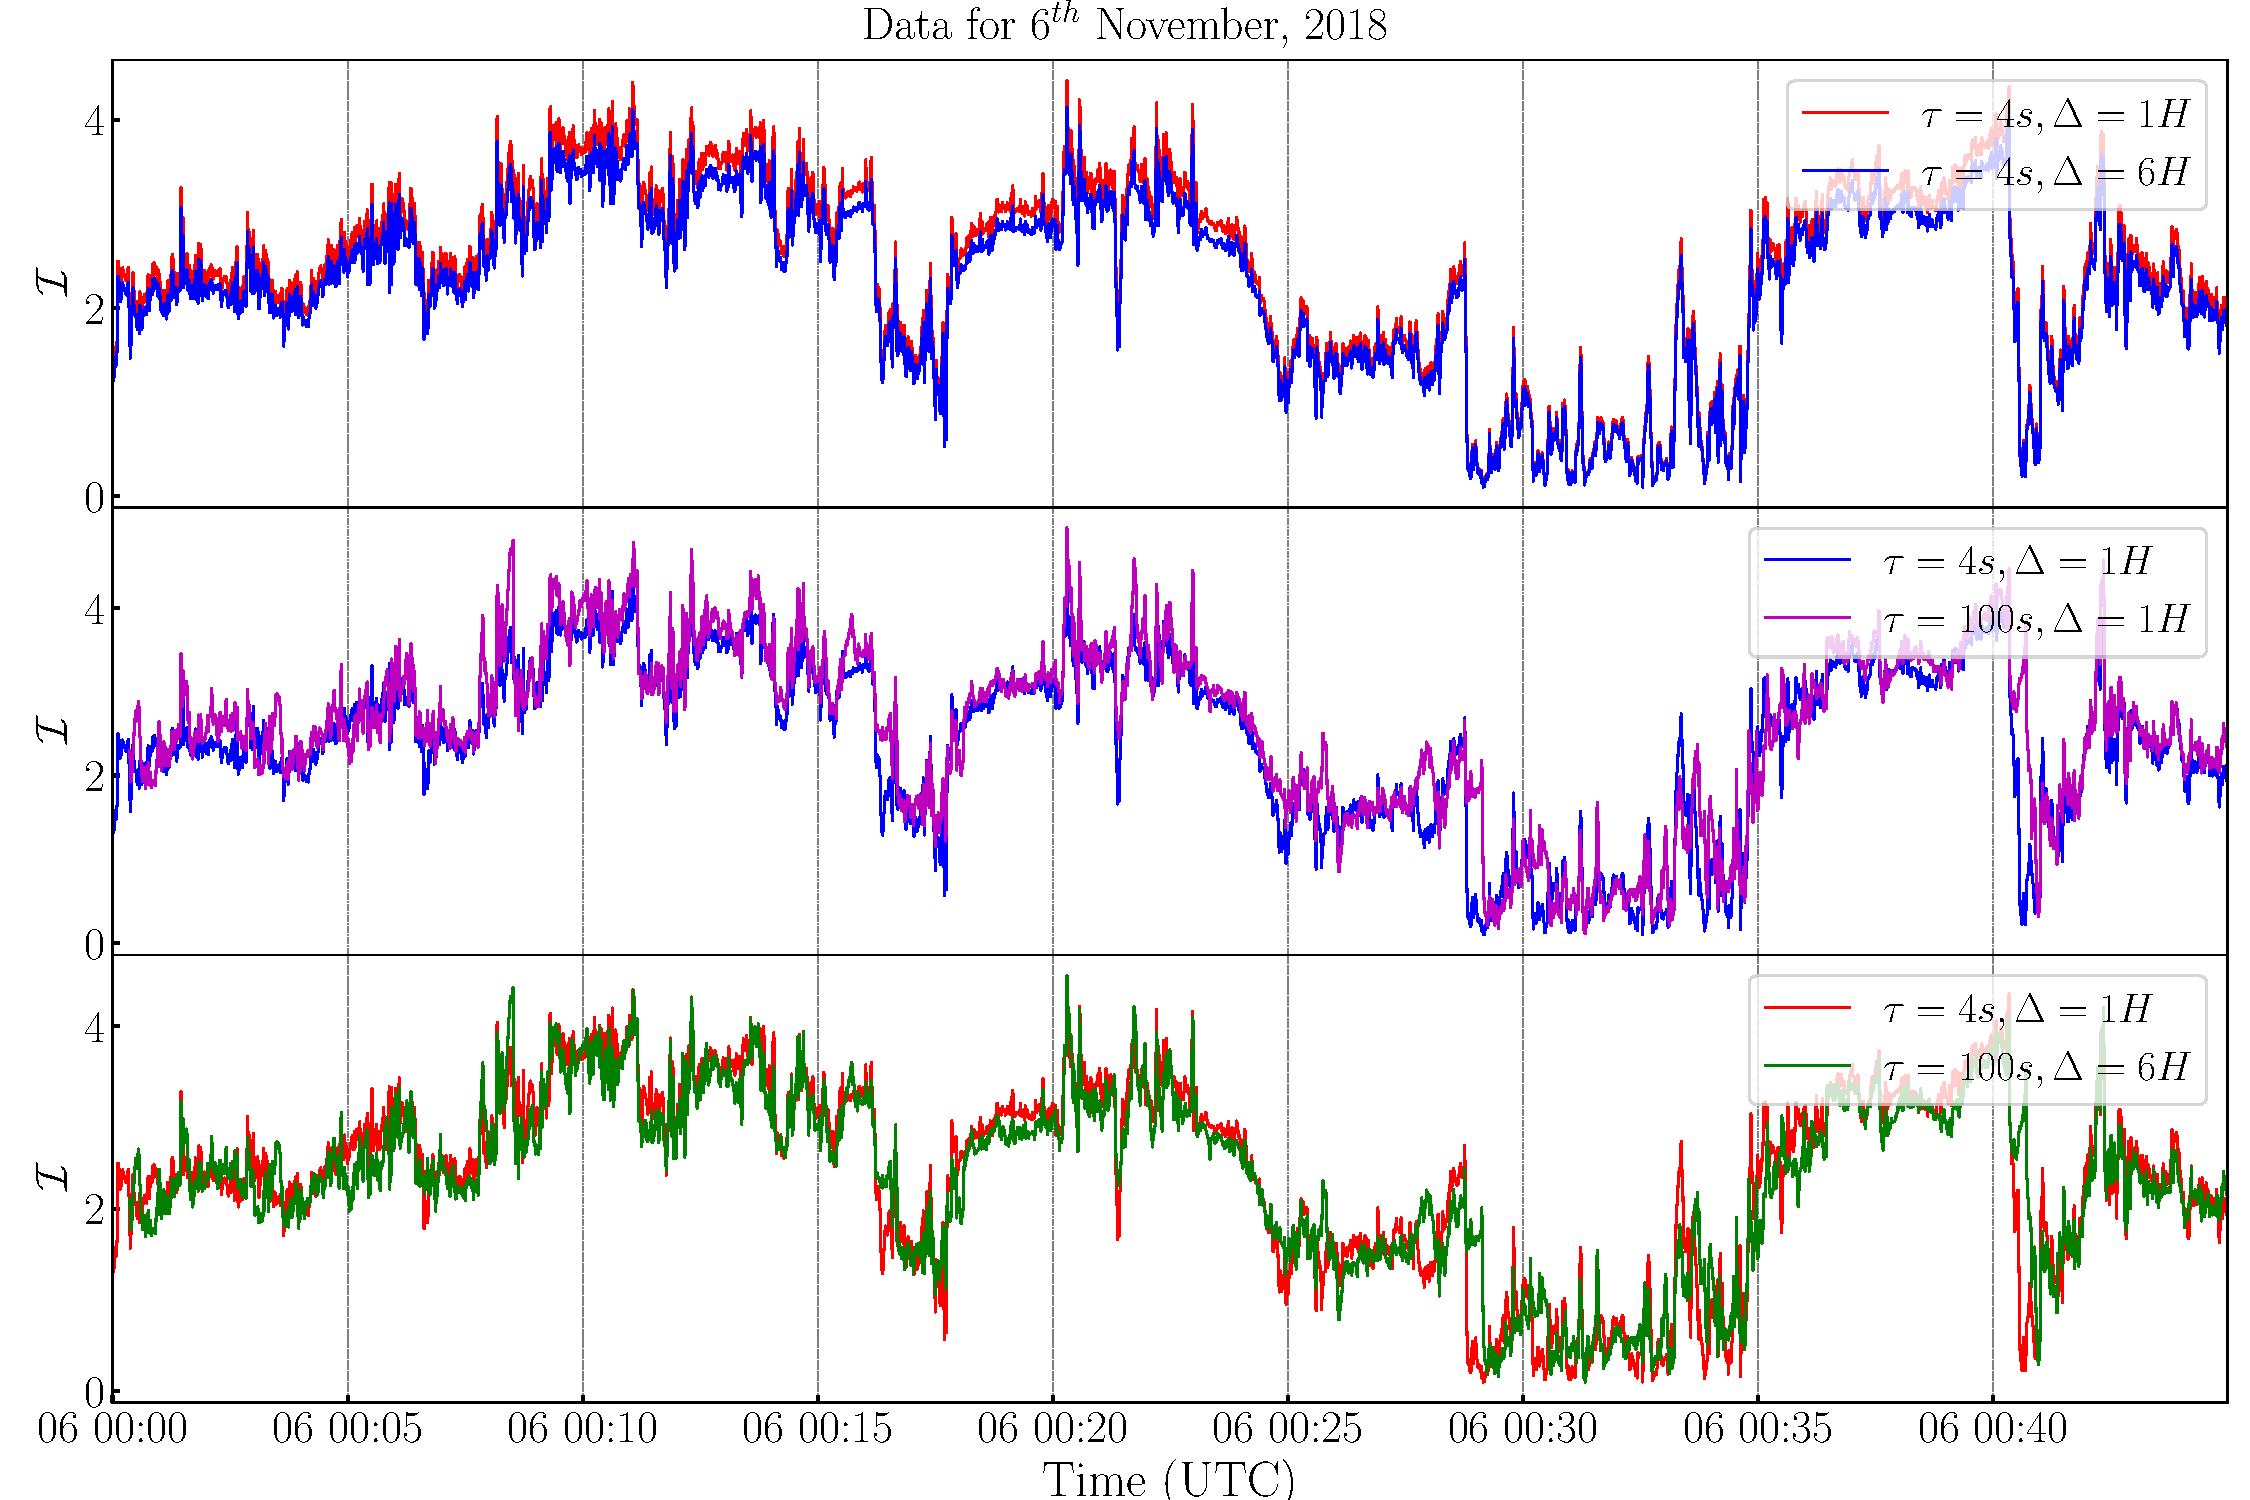
\includegraphics[width=1.\textwidth]{figures/chap6/pvi_comp_psp.pdf}
            \caption[$\mathcal{I}$ comparisons for different $\tau$]{Comparison of PVI computed for
            PSP for various different set of lag and averaging time. Though changing the lag or
            averaging times or both slightly changes the overall value of PVI, they remain highly
            correlated with respect to each other over time.}
            \label{fig:pvi_comp_psp}
        \end{sidewaysfigure}

        In this study we focused on the second half of the encounter, immediately after PSP was at
        its perihelion. The second half of the encounter has very different properties compared to
        the first half. A greater number of energetic particles were observed \citep{McComas2019},
        the solar wind speed was comparatively higher \citep{Kasper2019}, and there were many more
        switchbacks or polarity reversal of magnetic fields \citep{Bale2019}.
        \citet{Bandyopadhyay2020} observed enhanced local energy transfer, which points towards a
        more turbulent period in general, and thus a suitable environment for PVI study.

        For MMS analysis, we used the same data set as reported in \Cref{sec:sco5,sec:mms}.

    \section{Results} \label{sec:diss6}

        \begin{figure}
            \begin{center}
                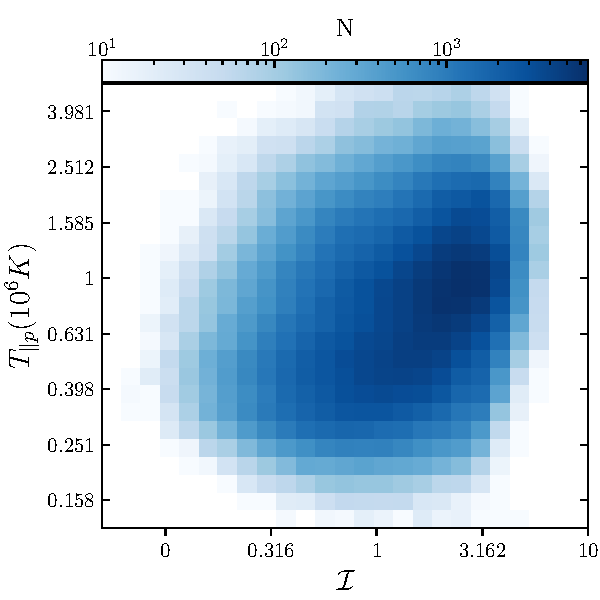
\includegraphics[width=1.\textwidth]{figures/chap6/PVIvsT_hist_masked_lin_mag_psp_par.pdf}
                \caption[Joint histogram of $T_{\parallel p}$ and $\mathcal{I}$]{Joint histogram of
                radial proton-temperature and PVI for the second half of first encounter on a
                log-log scale. There is an upward trend between PVI and temperature as the deep blue
                region in the plot tilts upwards showing an increase of temperature as PVI
                increases. \textit{Figure reproduced from \citet{Qudsi2020} with the permission of
                \href{https://publishing.aip.org/}{AIP Publishing}} (see
                \Cref{apdx:D}).}
                \label{fig:pvi_hst_psp}
            \end{center}
        \end{figure}

        \begin{figure}
            \begin{center}
                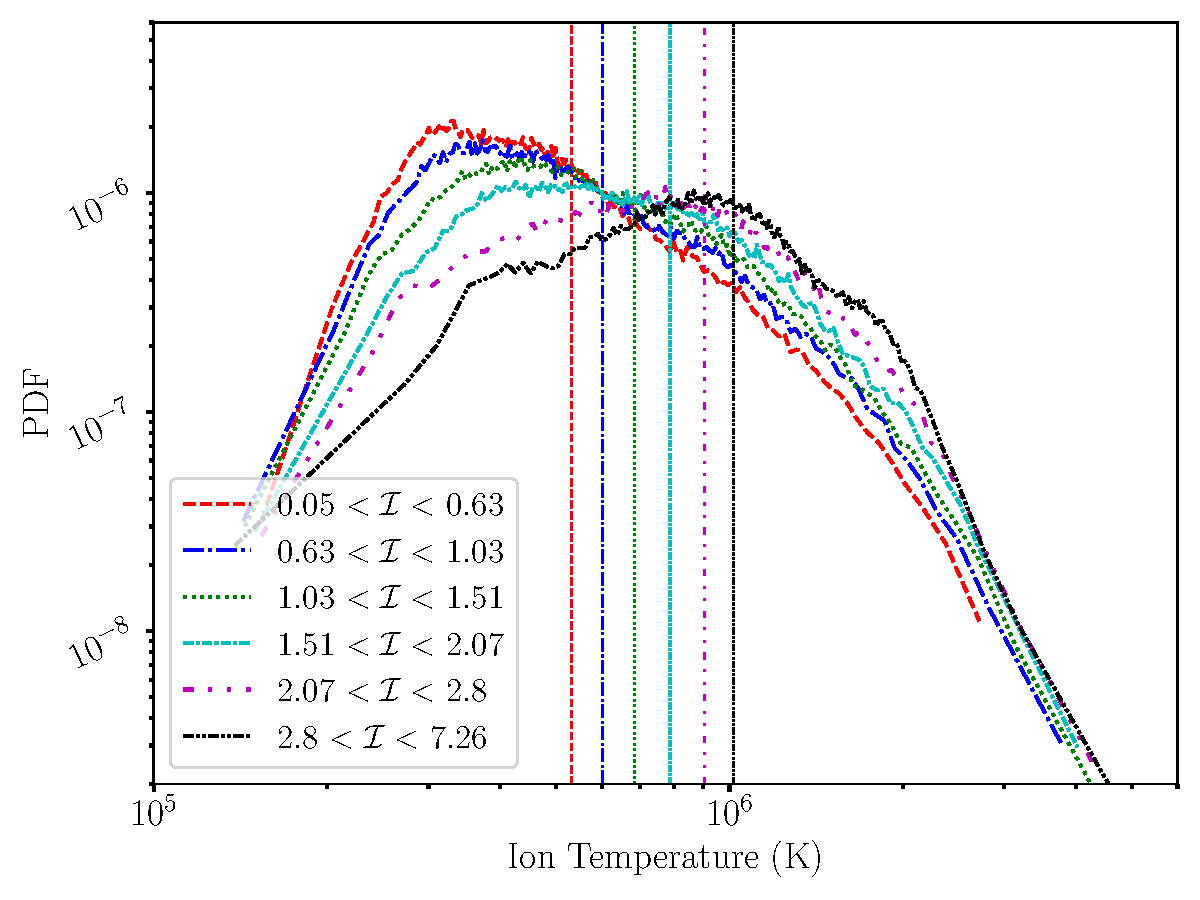
\includegraphics[width=1.\textwidth]{figures/chap6/T_pdf_pvi_psp.pdf}
                \caption[PDF of $T_{\rm \parallel p}$ for various $\mathcal{I}$ for \texttt{psp}
                dataset]{PDFs for the radial proton-temperature for the second half of first
                encounter. Each PDF corresponds to a different PVI range such that each PVI bin has
                equal number of data points. The probability density increases with increase in
                temperature for high PVI events and peaks at comparatively higher value of
                temperature, whereas it decreases for low PVI PDF. Vertical lines show the median
                temperature for each of the PDF plot. \textit{Figure reproduced from
                \citet{Qudsi2020} with the permission of \href{https://publishing.aip.org/}{AIP 
                Publishing}} (see \Cref{apdx:D}).}
                \label{fig:pvi_pdf_psp}
            \end{center}
        \end{figure}

        %\begin{figure} \begin{center}
        %    \includegraphics[width=1.\textwidth]{figures/chap6/%PVIvsT_hist_masked_lin_mag_mms_total.pdf}
        %    \caption{Joint histogram of total proton-temperature and PVI for the 40 minutes burst
        %    observation from MMS. Unlike the PSP case there doesn't seem to be a positive trend
        %    between temperature and PVI.} \label{fig:pvi_hst_mms} \end{center} \end{figure}

        \begin{figure}
            \begin{center}
                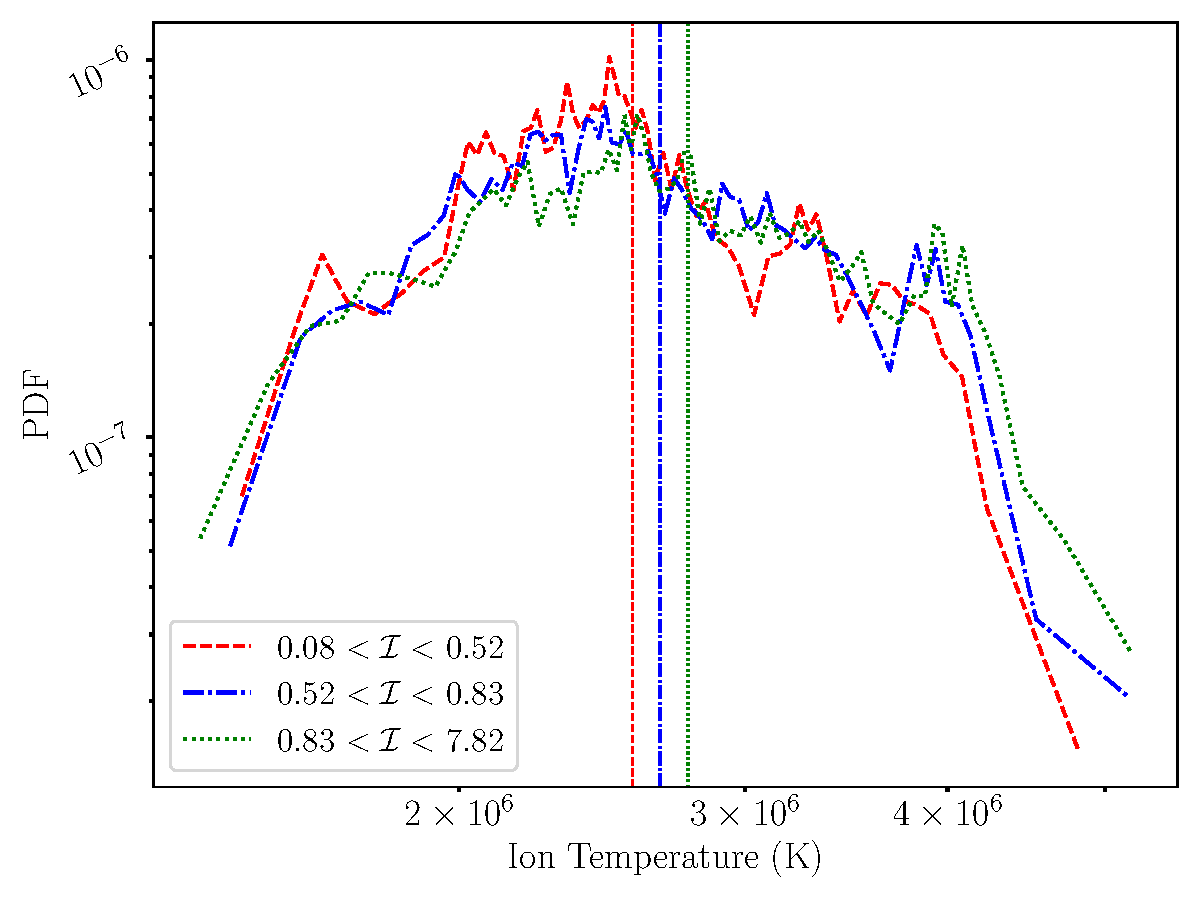
\includegraphics[width=1.\textwidth]{figures/chap6/T_pdf_pvi_mms_20171226_4.pdf}
                \caption[PDF of $T_{\rm \parallel p}$ for various $\mathcal{I}$ for \texttt{mms}
                dataset]{PDFs for the total proton-temperature for 40 minutes burst observation from
                MMS. Each PDF corresponds to a different PVI range such that each PVI bin has equal
                number of data points. The probability density increases with increase in
                temperature for high PVI whereas it decreases for low PVI PDF. Vertical lines show
                the median temperature for each of the PDF plot.}
                \label{fig:pvi_pdf_mms}
            \end{center}
        \end{figure}

        \Cref{fig:pvi_hst_psp} shows the joint histogram of radial proton-temperature and PVI for
        the first encounter of PSP. Increasing PVI color contours have an upwards trend, as we see
        temperature distribution showing a positive slope with increase in value of PVI. The
        positive correlation between temperature and PVI suggest some kind of heating in the regions
        with high PVI. We then conditionally sampled radial proton temperature. Conditionally
        sampled means that we arrange the data by increasing value of PVI and then divide all the
        data points in 6 bins such that each bin has equal number of points. We then calculate the
        temperature distribution within each bin which is shown in \Cref{fig:pvi_pdf_psp}.

        As PVI increases, the probability density increases for the higher temperature and decreases
        for the lower temperature which is opposite of what we see at the low temperatures where
        probability density is highest for the lowest PVI. Median temperature, shown by vertical
        lines in \Cref{fig:pvi_pdf_psp}, for each of the distribution increases implying presence of
        stronger and stronger heating as we go to higher and more extreme values of PVI. For PVI $<$
        1, median value of the temperature is $5.32 \times 10^5$\,K whereas for PVI $>$ 6, the
        median temperature increases to $1.01 \times 10^6$\,K. \citet{Osman2011} observed similar
        increase in average temperature in their study of solar wind at 1\,au. This is consistent
        with heating occurring in the regions with small scale coherent structure in MHD turbulence.

        Though distribution of total proton temperature from magnetosheath shows similar trend in
        the median temperature of each bin as seen in \Cref{fig:pvi_pdf_psp}, the enhancement in
        temperature is comparatively smaller. The median temperature corresponding to three bins
        shown in \Cref{fig:pvi_pdf_psp} are $2.56 \times 10^6$\,K, $2.66 \times 10^6$\,K and $2.77
        \times 10^6$\,K, which is barely an increment. However, this is reflective of two features
        of magnetosheath temperature and PVI compared to that of nascent solar wind. The radial
        temperature of solar wind varies over more than an order of magnitude whereas for
        magnetosheath it is less than half an order. Also, comparatively, solar wind has much higher
        values of PVI than that of magnetosheath, mean value of $1.69$ versus $0.78$. There are
        other factors to be considered as well. Short interval of observation which results in
        smaller amount of data could be another contributing factor. Also, in the case that
        fluctuation event lasts longer than the interval length, we won't detect any enhancement in
        the observed temperature. Though we did not see a conclusive evidence of temperature
        enhancement for ions, it is worth noting that \citet{Chasapis2018} did observe it for
        electrons. A comparative statistical study of PVI for datasets of different length of
        observation time will can help in quantifying how prominent is the effect of duration of
        observations on the value of computed PVI.

        In order to further demonstrate the relationship between PVI and enhanced temperature for
        PSP, we looked at the temperature at the point of high PVI event and its immediate
        surrounding in space using the methodology described by \citet{Osman2012a}. We compute the
        mean value of temperature at the point of the PVI event and for points near the PVI events
        separated from it by up to one correlation length. Formally, these averages may be expressed
        as:
        \begin{align}
            \widetilde{T}_{\rm p}( \delta t, \theta_{\rm 1}, \theta_{\rm 2}) = \langle T_{\rm p}(t_{\mathcal{I}}+\delta t)| \theta_{\rm 1} \leq \mathcal{I}(t_\mathcal{I}) < \theta_{\rm 2} \rangle \label{eq:tts}
        \end{align}
        where $\widetilde{T}_{\rm p}$ is the conditionally averaged temperature for all the events,
        $\delta t$ is the time difference relative to the position of PVI events, $t_\mathcal{I}$ is
        the time of PVI events between the threshold $\theta_{\rm 1}$ and $\theta_{\rm 2}$. In
        \Cref{eq:tts}, for a given threshold of PVI, we record the temperature at each point where
        PVI satisfies the expression $\theta_{\rm 1} \leq \mathcal{I}(t_\mathcal{I}) < \theta_{\rm
        2}$. We then record the temperature around that point, moving up to 1 correlation length
        away from the point of PVI event. Once we have the temperature at all such points, we take
        the average of all temperatures which were at same distance from the event.

        \begin{figure}
            \begin{center}
                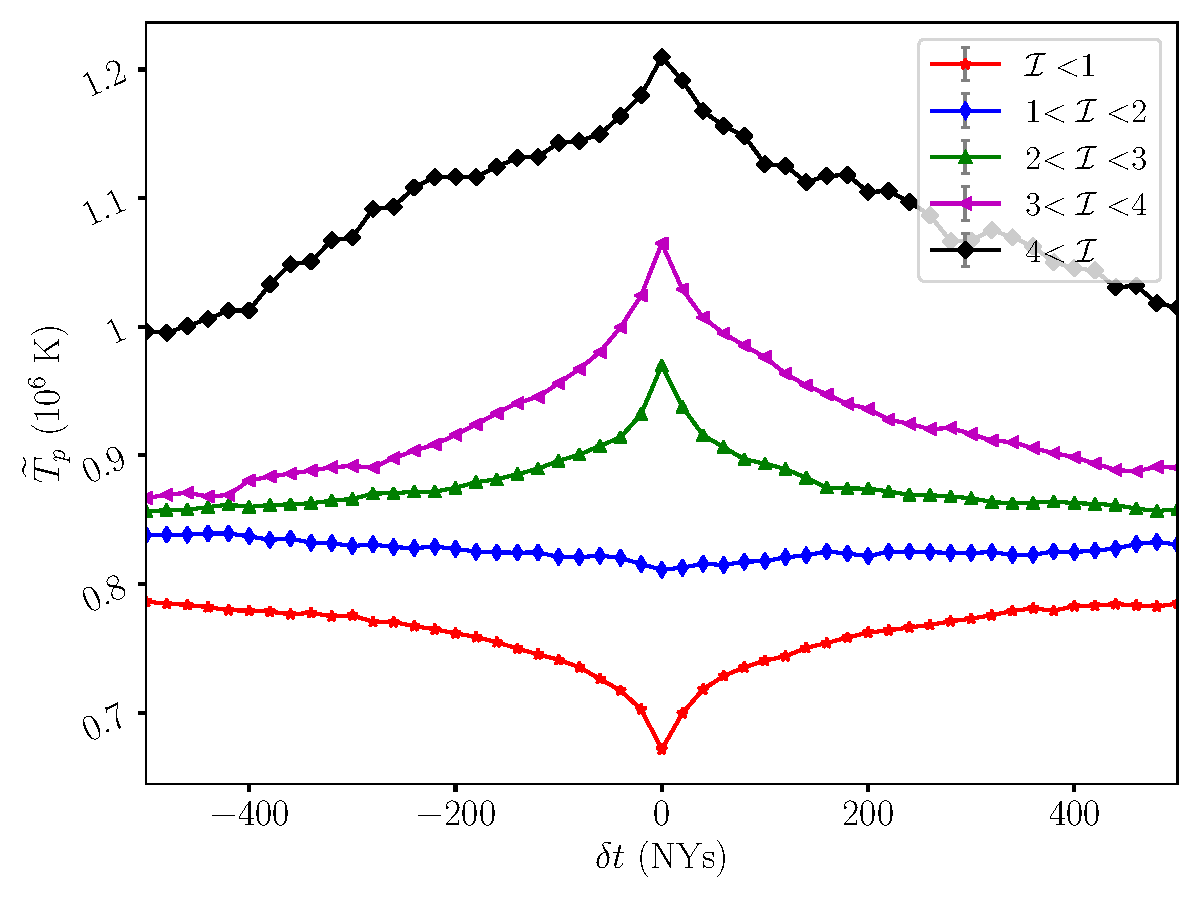
\includegraphics[width=1.\textwidth]{figures/chap6/tem_pvi_lag_psp.pdf}
                \caption[Conditionally averaged $T_{\rm \parallel p}$ from a $\mathcal{I}$
                event]{Figure shows conditional average temperature for different PVI thresholds at
                the point of a PVI event. $\widetilde{T}_{\rm p}$ peaks at the instant of PVI event
                and continues to have elevated temperature in its vicinity within the correlation
                time scale. Red curve, corresponding to lowest PVI shows a dip suggesting no heating
                when the magnetic field is very smooth. The error bars are smaller than the symbols
                and thus not easily visible in the figure. \textit{Figure reproduced from
                \citet{Qudsi2020} with the permission of \href{https://publishing.aip.org/}{AIP
                Publishing}} (see \Cref{apdx:D}).}
                \label{fig:tem_pvi_lag}
            \end{center}
        \end{figure}

        \Cref{fig:tem_pvi_lag} shows the plot of $\widetilde{T}_{\rm p}$ for various thresholds for
        the second half of the encounter. Not only do we observe enhanced temperature at the point
        of high PVI events, suggesting localized heating at those points, we also see that
        $\widetilde{T}_{\rm p}$ for a higher PVI event is consistently higher than nearby points
        separated by up to a correlation length. This implies that the points nearby an identified
        PVI event have an elevated average temperature, continuously approaching the elevated
        average temperature found at the PVI event itself. Some of this effect may be due to
        clustering of PVI events (see \citet{Chhiber2020}). Another point worth noting in
        \Cref{fig:tem_pvi_lag} is the valley in the temperature profile for small PVI. This is the
        region where background magnetic field is smooth and it appears that in such regions, the
        temperature is lower than the temperature of plasma in its immediate surrounding, which is
        concurrent with the fact that in those places there is no turbulence heating.
        \citet{Osman2012a} found similar result in their study at 1\,au. However, in our study we
        find a significant dip compared to the dip reported in \citet{Osman2012a}, $\sim 10^5$\,K
        compared to $\sim 2\times 10^3$\,K.

    \section{Discussions} \label{sec:conc6}

        In this study, we used in-situ observations from PSP's first encounter with the Sun and the
        magnetosheath data from MMS to explore the association of proton heating with coherent
        magnetic structures in space plasmas. We identified enhancements of PVI \citep{Greco2008} as
        indicative of the presence of such a structure \citep{Osman2011, Osman2012a}. We observed
        that the joint histogram of PVI and proton radial temperature, for solar wind, shows
        positive trend as shown in \Cref{fig:pvi_hst_psp}. We also observed that the PDF of data, as
        shown in \Cref{fig:pvi_pdf_psp,fig:pvi_pdf_mms}, with higher PVI has higher median
        temperature compared to those with lower PVI for both solar wind and terrestrial
        magnetosheath. These observations strongly supports the theory that the solar wind in those
        regions are heated by coherent structures which are generated by plasma turbulence. Though
        owing to certain characteristics of magnetosheath data, a more in-depth analysis is required
        to draw any final conclusion.

        The present results demonstrate both the shifting of the PDF of temperature towards higher
        values with increasing PVI condition, (in \Cref{fig:pvi_pdf_psp}) and the spatial/temporal
        localization of the temperature enhancement near PVI events (in \Cref{fig:tem_pvi_lag}).
        Both of these are fully consistent with findings in the two papers that examine these
        effects (\citet{Osman2011, Osman2012}, respectively). It is interesting that these effects
        are present clearly in the PSP first orbit where turbulence is presumably younger and
        possibly less well developed than it is at 1\,au. It is possible that the temperature
        differential between low and high PVI is somewhat less in the PSP data than in the ACE data
        at 1\,au \citep{Osman2011}, but additional samples by PSP will be needed to draw any firm
        conclusion of this type.

        In order to further demonstrate this association we looked at the conditionally average
        temperatures at the point of a high PVI event and in its immediate surrounding up to
        1\,correlation length. We observed that not only the point of event has the highest
        temperature, its vicinity shows enhanced temperature compared to lower PVI events. The local
        maxima of these temperature profiles are most prominent for higher PVI events suggesting
        stronger heating. The plateau region of each thresholds are distinct, and for higher
        threshold they maintain a high value suggesting clustering of PVI events around a large
        discontinuity. For very smooth magnetic field we see a dip in the average temperature at
        that point. \citet{Osman2012a} found similar behavior in their study of solar wind at 1\,au,
        though neither the heating nor the dip in temperature for small PVI that they reported in
        their study was as high as what we observed in our study. This suggests that either coherent
        structures are more efficient in heating the plasma near the Sun compared to 1\,au or we
        have a lot more such structures as we move closer to the Sun. Since these coherent
        structures are generated by plasma turbulence, these observations suggest that non-linear
        turbulence cascade play a crucial role in heating the nascent solar wind. Given the
        ubiquitous nature of such structures, this process can help explain the coronal heating or
        be at least a part of the explanation.

        A significant limitation of this study was unavailability of temperature-anisotropy data.
        The temperature measures we used were not the scalar temperature but rather the radial
        temperature, for which reason we limited our observations to period of nearly-radial
        magnetic field (see \Cref{sec:data6,sec:psp}). Once reliable ion temperature-anisotropy data
        are available, the present study could be revisited to explore both scalar and anisotropic
        heating. Theoretical studies have found that turbulent cascade can generate strong
        temperature anisotropy near coherent structures \citep{Parashar2016}.

        A careful inspection of \Cref{fig:tem_pvi_lag} reveals a very slight asymmetry in the shape
        of the temperature profile right before and after the PVI event. The phenomenon was also
        noted in 1\,au solar wind by \citep{Osman2012a}. The cause and significance of this
        asymmetry remain unclear, but it may it suggests a connection between local heating and
        large-scale processes such as heat flux.    % This file (chap6.tex) contains the text
                   % for Chapter 6.

%
% This is Chapter 7 file (chap7.tex)
%
\chapter{Interplay between linear and non-linear processes} \label{chap:chap7}

    \section{Overview} \label{sec:ovrvw7}

        In the last two chapters, \Cref{chap:chap4} and \Cref{chap:chap5}, we discussed two
        different processes which result in heating or temperature enhancements in the space
        plasmas. As we found in \Cref{chap:chap5} two processes occur simultaneously in both space
        and time and are entangled together at different scales. Consequently, there is an implied
        competition between the two processes to determine which one dominates given a set of
        conditions in the space plasmas. In this chapter we look at the two processes simultaneously
        to see the result of this competition as well as the dynamics between the two. We compare
        the time scales of two processes to see which one dominates and report our results in this
        chapter.\footnote{Part of this study was published in \citet{Bandyopadhyay2020b} and
        \citet{Gary2020}.}

    \section{Introduction} \label{sec:intr7}
    
        Solar wind is weakly collisional. The VDFs of solar wind ions exhibit non-Maxwellian
        features which introduce significant free energy in the system (see \Cref{chap:chap2}). The
        presence of additional features like secondary beam population\footnote{A field aligned
        secondary population of species which moves at a higher speed compared to the core
        population along the magnetic field lines.} \citep[and references therein]{Verscharen2019}
        signifies additional departure from the  local thermodynamic equilibrium and thus provide
        one form of free energy. All this often results in significant departure from temperature
        isotropy ($T_{\perp} = T_{\parallel}$), which leads to the development of kinetic
        microinstabilities\index{microinstability} fueled by the free energy in the system. As discussed in
        \Cref{chap:chap2,chap:chap5}, these instabilities then act to make the system more isotropic
        by scattering of particles in phase space.

        Turbulence is another process by which the opposite affect can be achieved, enhancement in
        anisotropy of the plasma, and because of its ubiquitous nature, it is expected to play
        important role in the dynamics of the plasmas. Thus at any point these two processes are
        either feeding off of each other or are competing in the system. Recent studies have shown
        that coherent structures (e.g., current sheets) generated by solar wind turbulence can
        generate extreme anisotropies \citep{Greco2012,Servidio2015,Karimabadi2013} which results in
        development of linear growth rates as predicted by the Vlasov dispersion equation
        \citep{Qudsi2020a}. Other studies \citep{Karimabadi2013,Matthaeus2015} have shown that local
        instabilities may arise occasionally in the presence of shear driven turbulence\index{turbulence}.
        \citet{Bale2009} found enhancements in magnetic fluctuations in regions of solar wind plasma
        that are susceptible to the development of one or more microinstabilities. \citet{Osman2013}
        showed the presence of high cascade rate in the same regions, suggesting that these two,
        linear and non-linear, processes exist in the same space.

        However, since these two processes compete with each another to influence the plasma, it
        remain unclear as of now which one dominates and drive the large scale phenomenon. We thus
        decided to study the time scales at which the two processes work and compare them in
        different types of plasmas. For kinetic microinstabilities we study the linear growth rates
        (see \Cref{sec:instab2}) whereas for time scales associated with turbulence we look at the
        non-linear frequency and time scales as computed in \Cref{sec:nlts}. We carry out this
        analysis for six different datasets: 3 from simulation and 3 from in-situ measurement of
        space plasmas (see \Cref{chap:chap4} and \Cref{tab:datachap} for details of data and some
        other relevant quantities).

    \section{Data Selection and Methodology} \label{sec:data7}

        Since we are to compare the two time scales, we look at the linear and non-linear rates
        present in the plasma locally. For the linear growth rates, we consider all the four growth
        rates\footnote{Under the assumption of no secondary beam populations and an isotropic
        electron population.} which might be active at any point and compute the maximum of the 4
        rates, where each growth rate was computed by the method described in
        \Cref{sec:cgr,sec:intr42}. \Cref{eq:lin_max_gamma} puts this succinctly in the form of an
        equation.
        \begin{align}
            \Gamma_{\max} & = \max\left( \gamma_{\rm \max, cyclotron}, \gamma_{\rm \max, mirror}, \gamma_{\rm \max, \parallel firehose}, \gamma_{\rm \max, \nparallel firehose} \right) \label{eq:lin_max_gamma}
        \end{align}
        For the non-linear rate, we computed the local nonlinear frequency\index{Frequency!nonlinear} ($\omega_{\rm nl}$) at
        any position \textbf{r} for a lag length scale of $\ell$ as :
        \begin{align}
            \omega_{\rm nl} \sim \delta b_l/\ell \label{eq:nln_time}
        \end{align}
        Where $\delta b_\ell$ is the change in the longitudinal magnetic field and is given by :
        \begin{align}
            \delta b_{\ell} = \left \lvert\hat{\boldsymbol{\ell}} \mathbf{\cdot} \left[\mathbf{b} (\mathbf{r} + \boldsymbol{\ell}) - \mathbf{b} (\mathbf{r})\right]\right\lvert \label{eq:db2},
        \end{align}
        Where \textbf{b} is the total magnetic field expresses in local Alfv\'en speed units (see
        \Cref{sec:nlts}). As mentioned in \Cref{sec:2pic} for all cases except the 3-D dataset,
        since the goal was to carefully evaluate the nonlinear frequency at the scale of the fastest
        growing mode, the value of $\ell$ is given by $1/k_{\max}$, where $k_{\max}$ is the wave
        number corresponding to $\Gamma_{\max}$ as computed in \Cref{eq:lin_max_gamma}. Since for
        marginally unstable plasma, $k_{\max}$ is typically of the same order as the ion inertial
        length ($d_{\rm i}$) \citep[Figures 6.6 to 6.9]{Maruca2012a}, for the case of 3-D
        simulation, because of some computation limitation, we set $\ell = d_{\rm i}$.

    \section{Results} \label{sec:diss7}

        \Cref{fig:ratio_allsim} shows the comparison between the two time scales (linear and
        non-linear) for three different simulations (see \Cref{chap:chap4} for more detail). The
        first panel of each row shows the maximum value of linear growth rates
        $\left(\Gamma_{max}\right)$ as defined by \Cref{eq:lin_max_gamma}. The second panel shows
        the non-linear growth rates $\left(\omega_{\rm nl}\right)$ computed using
        \Cref{eq:nln_time}. Though $\omega_{\rm nl}$ is largely uniform over the simulation box,
        heightened values of it lie close to the regions with high current density and/or where
        temperature anisotropy has extreme values (see \Crefrange{fig:brjhb}{fig:brjros}). The third
        panel shows the ratio between the two growth rates. This ratio is only computed for regions
        where the condition $\Gamma_{\max} > 10^{-5}\Omega_{\rm cp}$ is satisfied, consequently
        there are very few points of comparison compared to the total number of points inside the
        box (see \Cref{tab:ngamma}). The third panel shows that there are very few points where
        $\Gamma_{\max} > \omega_{\rm nl}$, which implies the dominance of non-linear phenomena over
        the linear one for all three different kinds of simulation conditions. This means that it
        takes longer time for the linear instability to affect the system than the eddy turnover
        time and thus it will be the nonlinear processes and not linear instability which will
        dictate the evolution of the system. Counting the number of data points where both the
        conditions ($\Gamma_{\max} > 0$ and $\Gamma_{\max}/\omega_{\rm nl} > 1$) were satisfied, we
        found that the conditions were true only for 0.019, 0.053 and 0.59 percentages of cases for
        \texttt{149p6}, \texttt{kaw} and \texttt{ros} datasets respectively.
        
        \begin{table}[ht]
            \centering
            \caption[Dataset detail for $\Gamma_{\max}$ and $\omega_{\rm nl}$]{Number of points in
            each datasets, and where we have active linear instability present ($\Gamma_{\max} >
            10^{-5}\,\Omega_{\rm cp}$) and where $\Gamma_{\max}/\omega_{\rm nl} > 1$ with associated
            percentages in parenthesis}
            \begin{tabular}{  m{0.15\linewidth}  m{0.25\linewidth}  m{0.25\linewidth}
            m{0.25\linewidth}}
                \hline
                \\
                \multirow{2}{\linewidth}{Datasets} & \multicolumn{3}{|c|}{Number of } \\
                \cline{2-4}
                & total data points & points where \newline $\Gamma_{\max} > 10^{-5}\,\Omega_{\rm
                cp}$ (\%) & points where \newline $\Gamma_{\max}/\omega_{\rm nl} > 1$ (\%)\\
                \hline
                \\
                \texttt{149p6} & 16,777,216 & 1,144,615 (6.82) & 3,347 (0.019)\\ \\
                \hline
                \\
                \texttt{kaw} & 4,194,304 & 37,560 (0.90) & 2,227 (0.053) \\ \\
                \hline
                \\
                %20160125 & & & \\
                %\hline
                \texttt{ros} & 134,217,728 & 22,001,875 (16.39) & 794,220 (0.59) \\ \\
                \hline
                \\
                %20170127 & & & \\
                %\hline
                \texttt{mms} & 15,857 & 3,887 (24.51) & 174 (1.10)\\ \\
                \hline
                \\
                \texttt{wnd} & 1,316,621 & 187,338 (14.22) & 2,7857 (2.11) \\ \\
                \hline
                \\
                \texttt{psp} & 95,034 & 5,347 (5.62) & 1,483 (1.56) \\ \\
                \hline
            \end{tabular}
            \label{tab:ngamma}
        \end{table}

        \begin{sidewaysfigure}
            \begin{center}
                \includegraphics[width=0.95\textheight]{figures/chap7/all_sim_gamma_omega_ratios_blues.pdf}
                \caption[Comparison plot of $\Gamma_{\max}$, $\omega_{\rm nl}$ and
                $\Gamma_{\max}/\omega_{\rm nl}$ for simulations]{Plots (from left to right) of
                maximum linear growth rate ($\Gamma_{\max}$), nonlinear frequency ($\omega_{\rm
                nl}$) and the ratio $\Gamma_{\max}/\omega_{\rm nl}$ for the three different kinds of
                PIC simulation. First row shows the data for \texttt{149p6} dataset, middle row is
                for \texttt{kaw} dataset and the bottom row shows the data from \texttt{ros}
                dataset.}
                \label{fig:ratio_allsim}
            \end{center}
        \end{sidewaysfigure}

        \Crefrange{fig:ratio_mms}{fig:ratio_psp} show the time series equivalent of
        \Cref{fig:ratio_allsim} for three different spacecraft (MMS, Wind and PSP respectively),
        located in different space plasmas: Earth's magnetosheath, 1\,au solar wind, and near-Sun
        solar wind ($\sim$ 0.2\,au) (see \Cref{sec:plas2} and \Cref{chap:chap4}). Similar to
        \Cref{fig:ratio_allsim}, for each of these figure the first panel shows the time series for
        $\Gamma_{\max}$, the second shows that for $\omega_{\rm nl}$, and the third shows ratio of
        the two. The dashed red line in each third panel demarcates $\Gamma_{\max} = \omega_{\rm
        nl}$. Though in all three sets of observations, fraction of data with $\Gamma_{\max} >
        \omega_{\rm nl}$ is higher than in the simulations (see \Cref{tab:ngamma}), it remains well
        below 50\%. Though \citet{Klein2018} used a different method to compute the condition of
        plasma instability and a different condition for calculation of $\omega_{\rm nl}$, they
        found a similar result for solar wind at 1\,au.
        \begin{sidewaysfigure}
            \begin{center}
                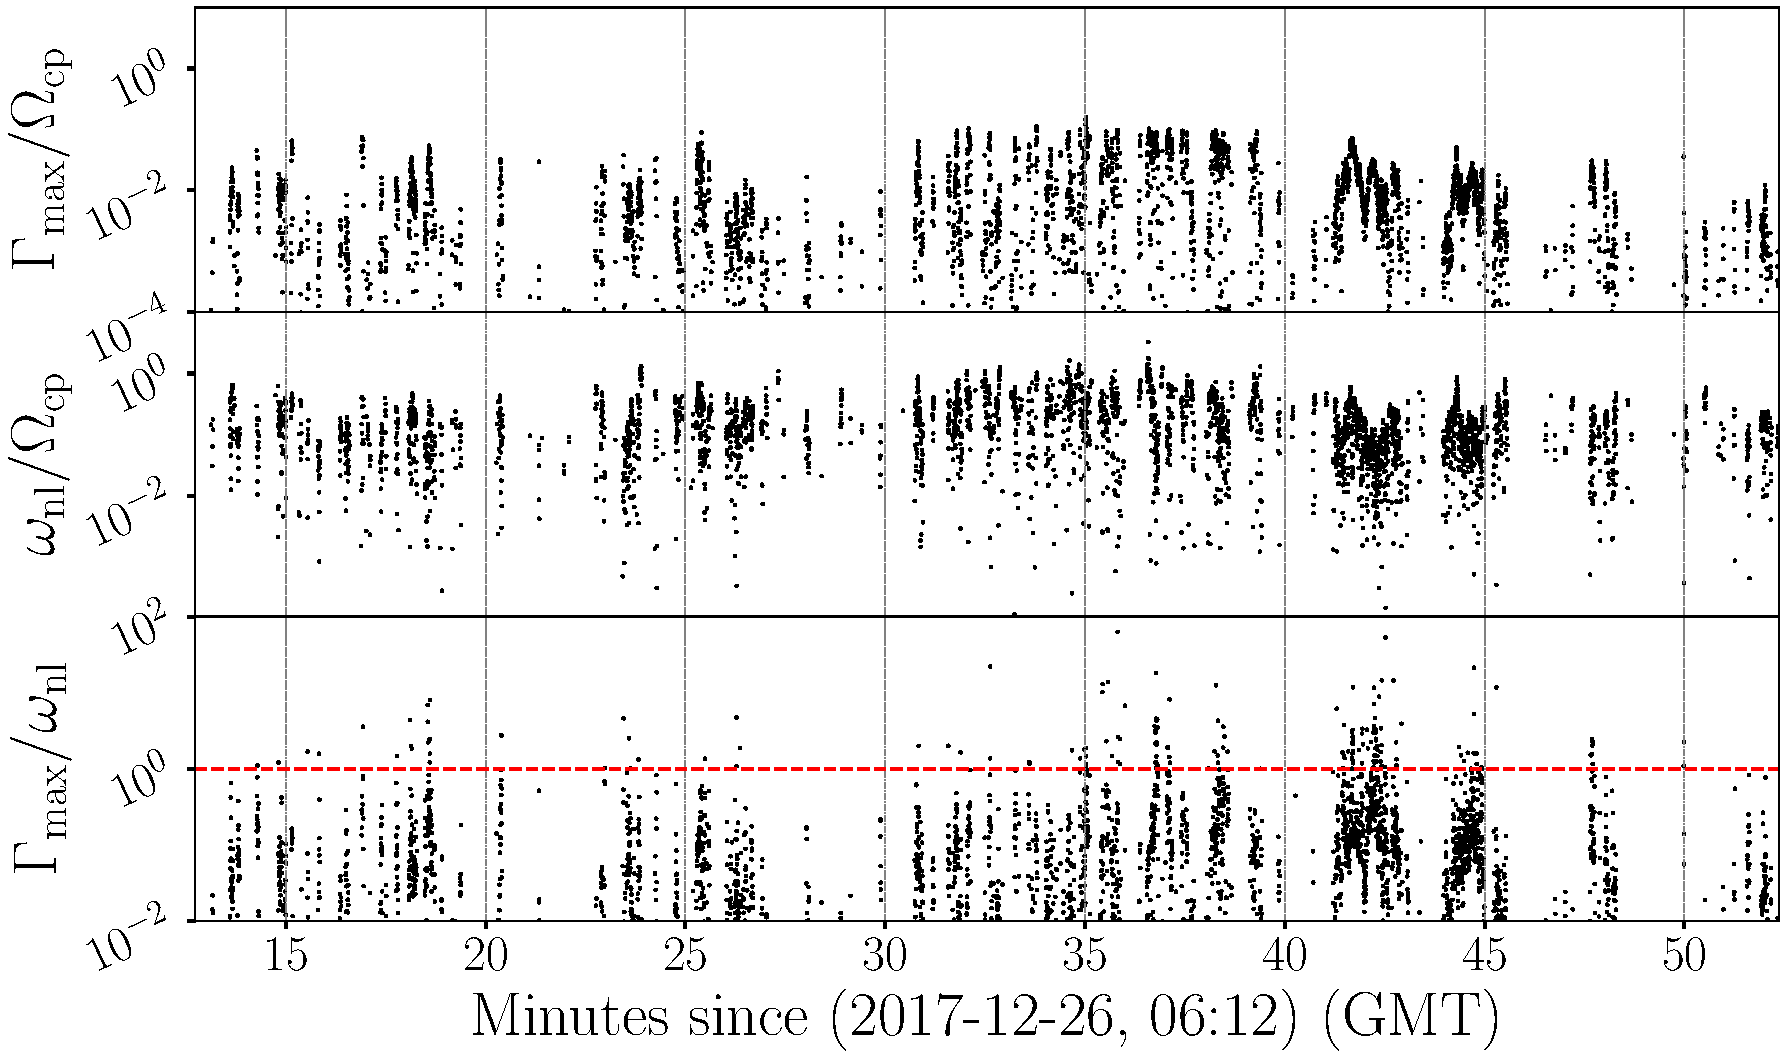
\includegraphics[width=1.\textwidth]{figures/chap7/mms_gamma_omega_ratio_2017-12-26_2017-12-26_00000000_00015856.pdf}
                \caption[Comparison plot of $\Gamma_{\max}$, $\omega_{\rm nl}$ and
                $\Gamma_{\max}/\omega_{\rm nl}$ for \texttt{mms} dataset]{Time series plot of (top
                to bottom) of maximum linear growth rate ($\Gamma_{\max}$), nonlinear frequency
                ($\omega_{\rm nl}$) at 1\,$d_{\rm i}$, and the ratio $\Gamma_{\max}/\omega_{\rm nl}$
                at z\,=\,0.\,$d_{\rm i}$ from terrestrial magnetosheath.}
                \label{fig:ratio_mms}
            \end{center}
        \end{sidewaysfigure}

        \begin{sidewaysfigure}
            \begin{center}
                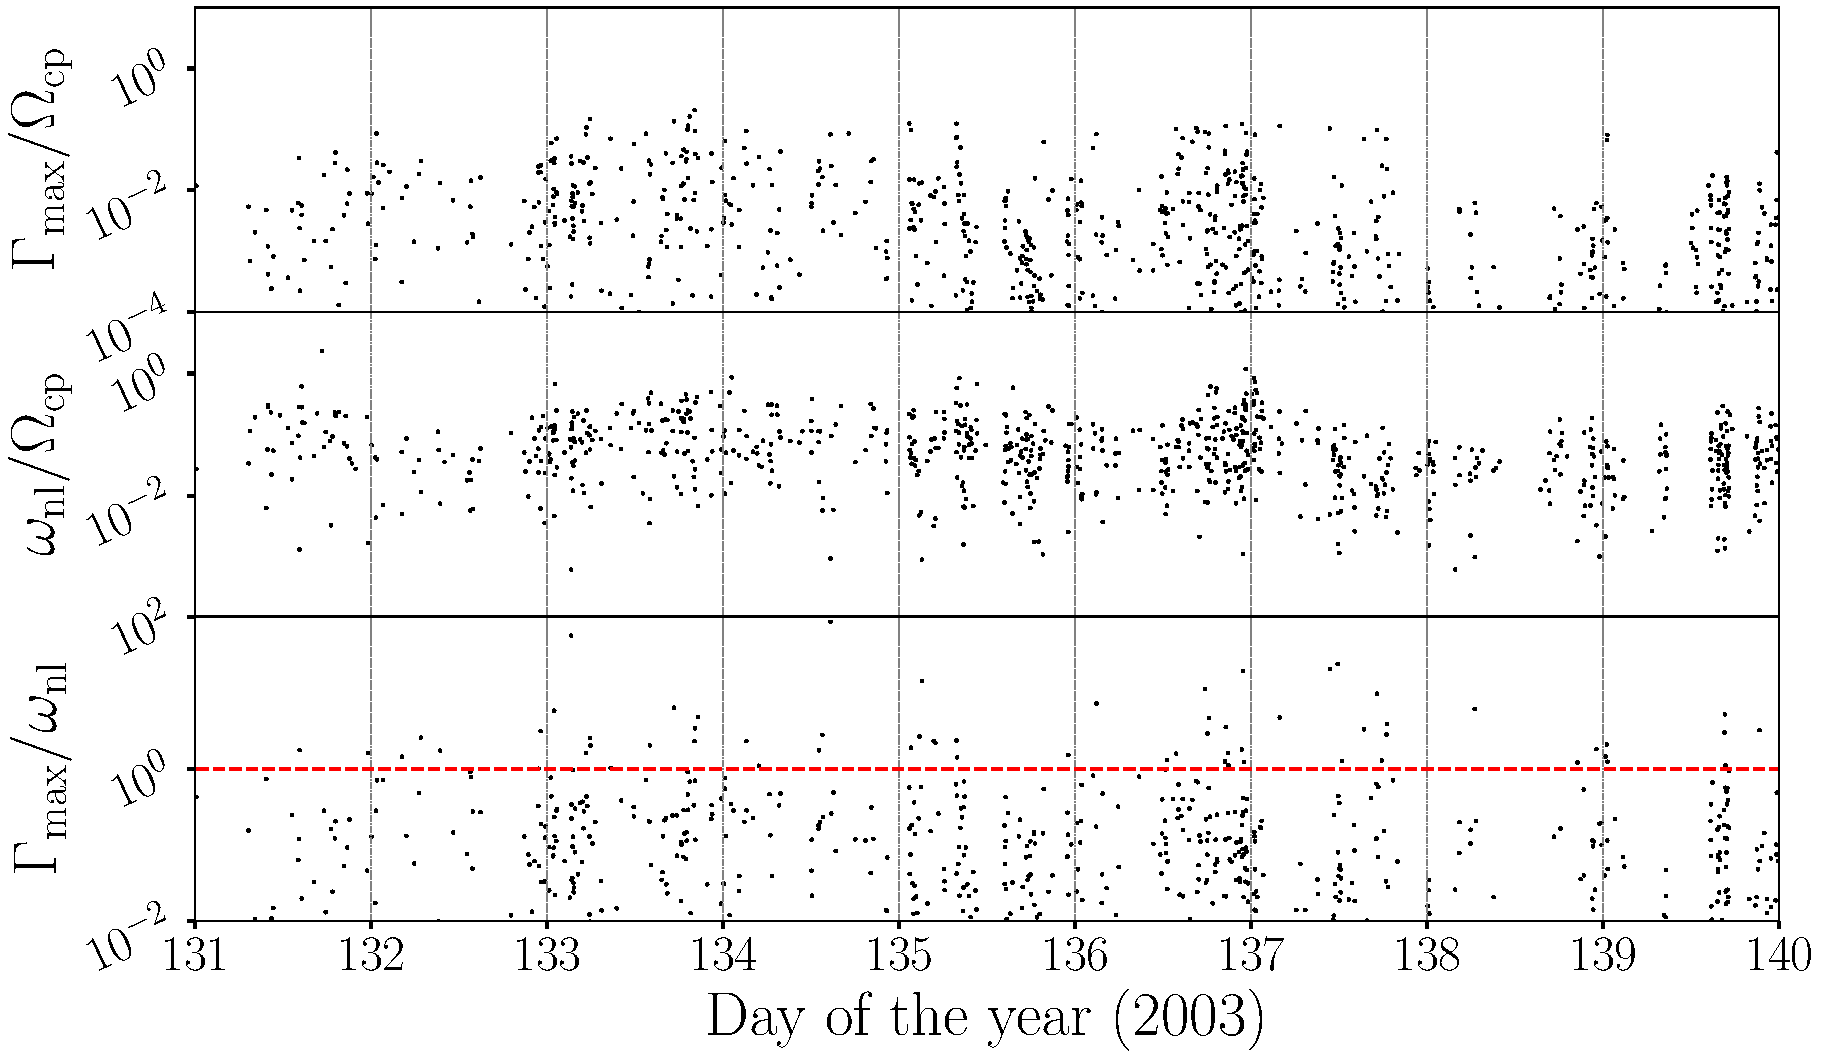
\includegraphics[width=1.\textwidth]{figures/chap7/wnd_gamma_omega_ratio_2003-5-11_2003-5-19_01207878_01212368.pdf}
                \caption[Comparison plot of $\Gamma_{\max}$, $\omega_{\rm nl}$ and
                $\Gamma_{\max}/\omega_{\rm nl}$ for \texttt{wnd} dataset]{Time series plot of (top
                to bottom) of maximum linear growth rate ($\Gamma_{\max}$), nonlinear frequency
                ($\omega_{\rm nl}$) at 1\,$d_{\rm i}$, and the ratio $\Gamma_{\max}/\omega_{\rm nl}$
                at z\,=\,0.\,$d_{\rm i}$ from solar wind at 1-au.}
                \label{fig:ratio_wnd}
            \end{center}
        \end{sidewaysfigure}

        \begin{sidewaysfigure}
            \begin{center}
                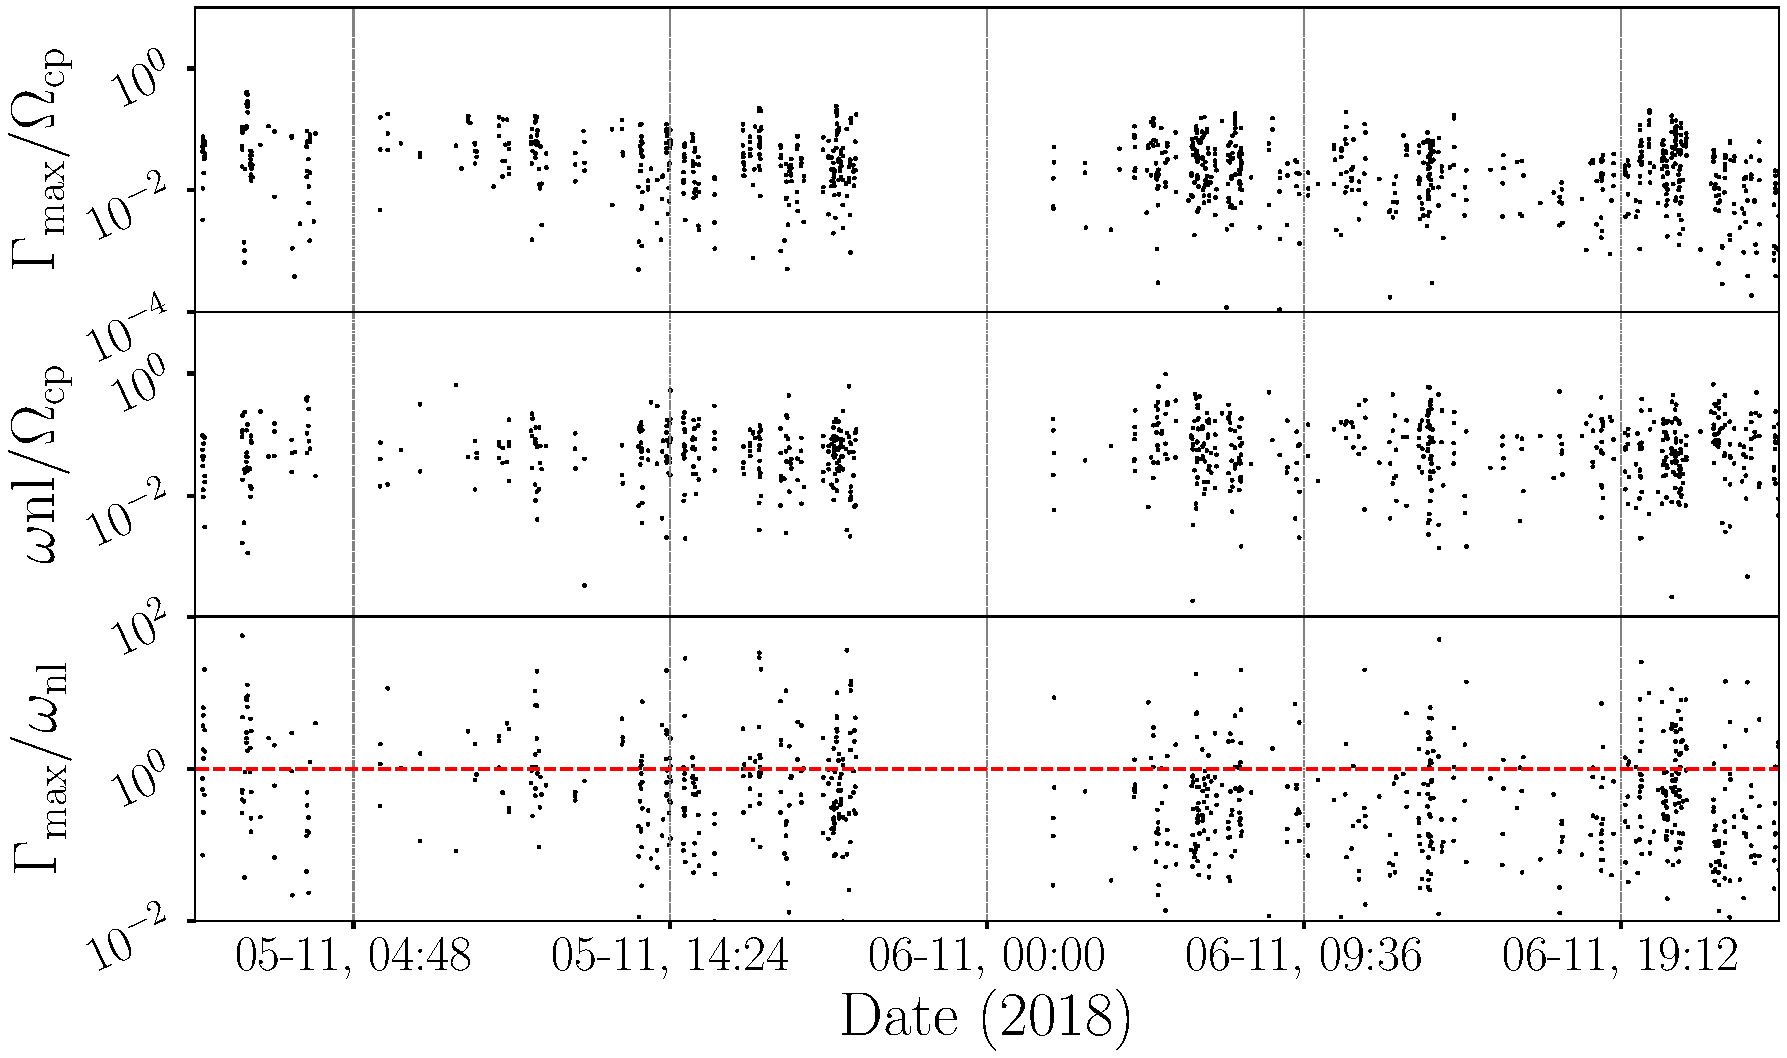
\includegraphics[width=1.\textwidth]{figures/chap7/psp_gamma_omega_ratio_2018-11-5_2018-11-7_00043197_00060477.pdf}
                \caption[Comparison plot of $\Gamma_{\max}$, $\omega_{\rm nl}$ and
                $\Gamma_{\max}/\omega_{\rm nl}$ for \texttt{psp} dataset]{Time series plot of (top
                to bottom) of maximum linear growth rate ($\Gamma_{\max}$), nonlinear frequency
                ($\omega_{\rm nl}$) at 1\,$d_{\rm i}$, and the ratio $\Gamma_{\max}/\omega_{\rm nl}$
                at z\,=\,0.\,$d_{\rm i}$ from solar wind close to the Sun.}
                \label{fig:ratio_psp}
            \end{center}
        \end{sidewaysfigure}
        \Cref{fig:ratio_kde_all} shows the kernel density estimate (KDE) \footnote{KDE is a
        non-parametric method of probability density estimation of a random variable.} plot for each
        of the aforementioned six datasets generated using \texttt{seaborn} package in Python. As
        expected, in all the cases the core of KDE is below $\Gamma_{\max} = \omega_{\rm nl}$ line
        (dashed red line). Though for simulation dataset \texttt{149p6} the core of the distribution
        is centered between $\Gamma_{\max} = 10^{-4}$ and $\Gamma_{\max} = 10^{-3}$, for both
        \texttt{kaw} and \texttt{ros} datasets centroid of KDE is more than an order of magnitude
        higher at $\Gamma_{\max} = 10^{-2}$. This can be attributed to the fact that in both of
        these simulations the background magnetic field ($\mathbf{B_{\rm 0}}$) in the plane of the
        fluctuations is non-zero, by design for the \texttt{kaw} dataset and for \texttt{ros}
        dataset because there are fluctuations in all 3 directions. This results in the case that
        $\textbf{k}_\parallel \neq 0$ for these two simulations, whereas for \texttt{149p6}
        simulation since there is no spatial variation in the direction parallel to $\mathbf{B_{\rm
        0}}$, wave vector components parallel to $\mathbf{B_{\rm 0}}$ are zero. This results in
        limited application of both Landau (fluctuations of zero frequency) and cyclotron resonance
        (fluctuations with $n^{th}$ species cyclotron frequencies)\citep{Gary2020}. This makes both
        the resonances independent of particle velocities and thus the particles are constrained to
        fluid-like behavior. Because of this, \texttt{149p6} simulation fails to account for
        velocity dependent wave-particle interactions which may represent critical elements of
        turbulent dissipation at wavelengths of the order of or shorter than $d_{\rm
        i}$\citep{Gary2020}.
        \begin{sidewaysfigure}
                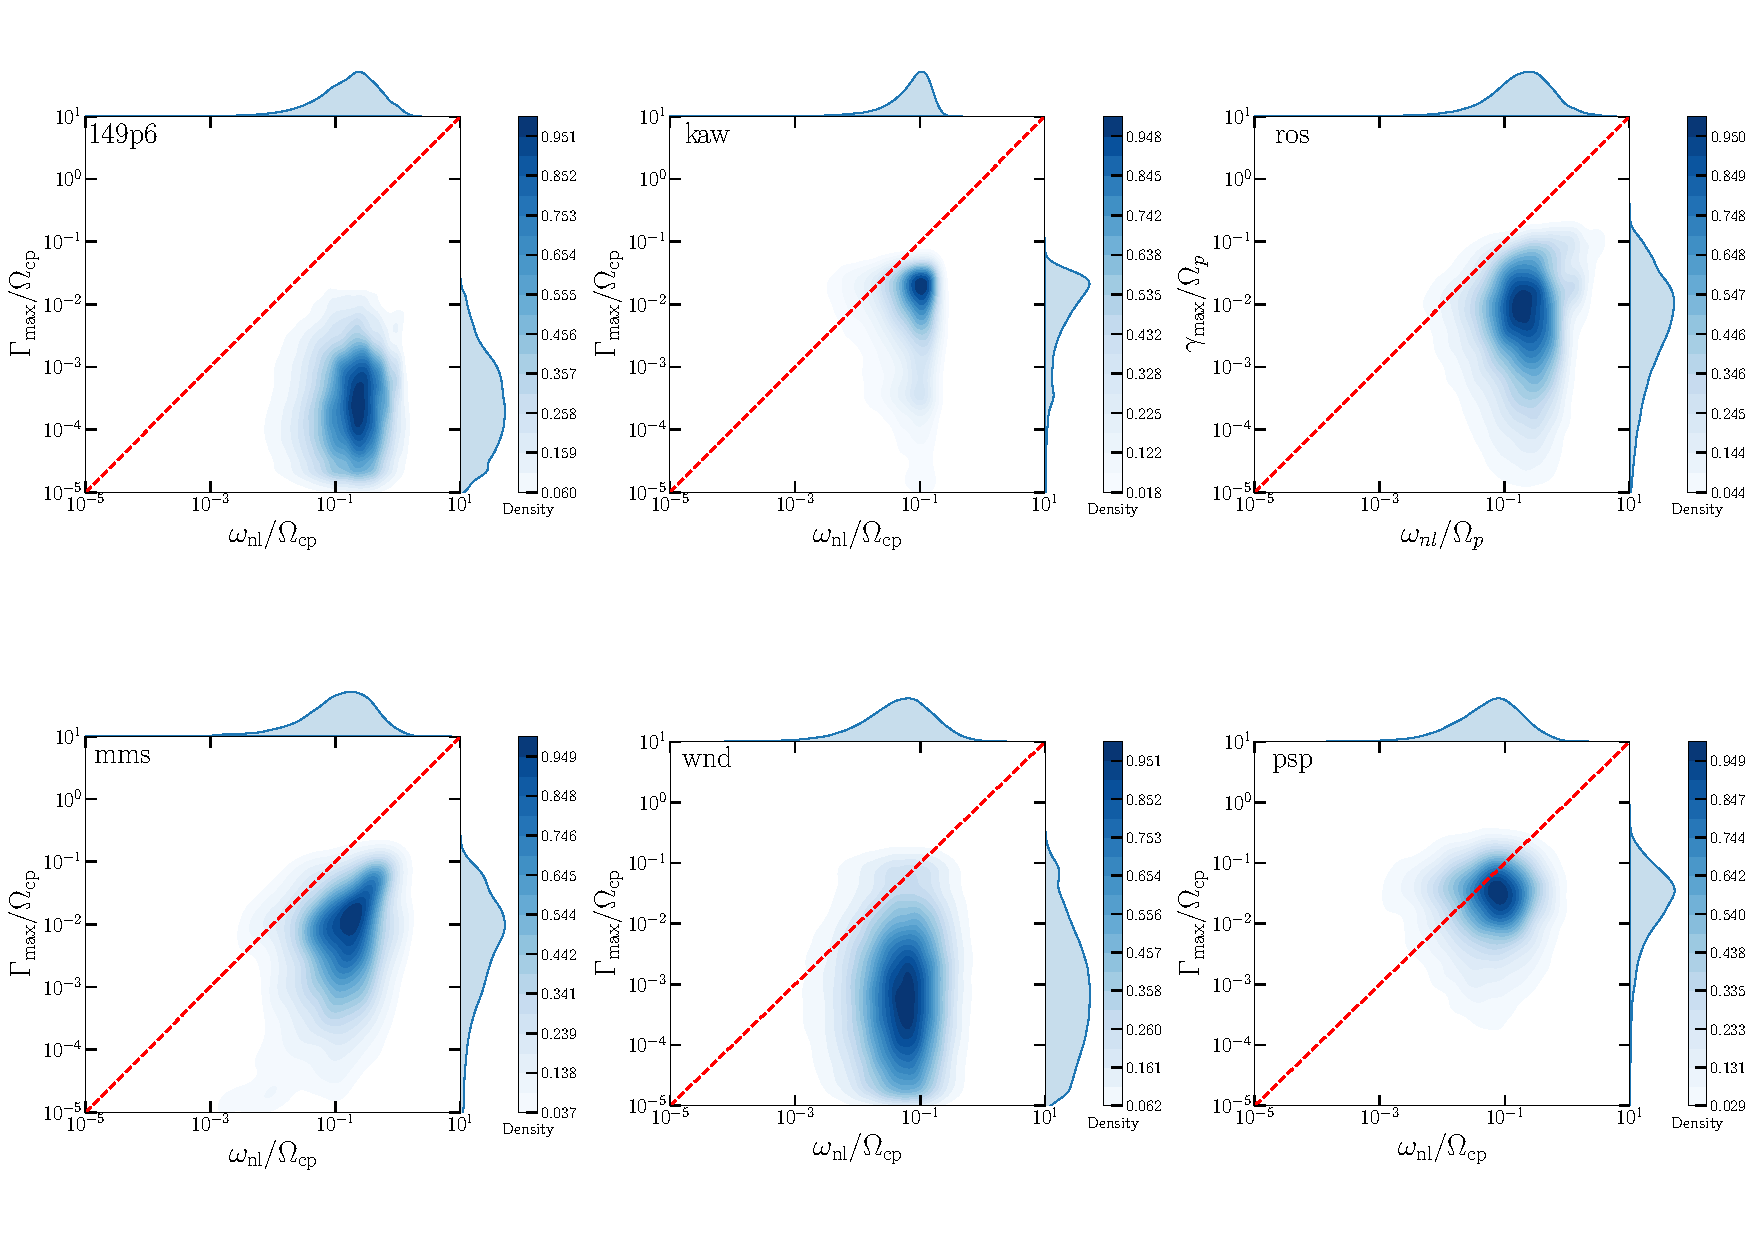
\includegraphics[width=1.\textwidth]{figures/chap7/kdeplots_merged_v9.pdf}
                \caption[KDE plots for all six datasets]{Kernel density plot for all six datasets
                used in this study. For all the cases the centroid of distribution is well below the
                $\Gamma_{\max} = \omega_{\rm nl}$} line, shown as dashed-red line, implying the
                dominance of non-linear processes over linear ones in all kind of plasmas.
                \label{fig:ratio_kde_all}
        \end{sidewaysfigure}
        Another interesting feature of these KDE plots is how much closer to the $\Gamma_{\max} =
        \omega_{\rm nl}$ line the centroid of the distribution is for the PSP data compared to other
        spacecraft data, implying substantially more competition between the linear and non-linear
        processes closer to the Sun. \citet{Klein2021} observed similar enhancements in the linear
        growth rates for plasma closer to the Sun. Further analysis is needed, though, since the
        available PSP data were from such a short time interval (see \Cref{sec:psp}), and
        temperature anisotropy was computed using an entirely novel technique  \citep{Huang2020}. As
        was remarked in \Cref{sec:conc6} close to the Sun the turbulence is quite young and not
        developed enough implying presence of weaker non-linear instabilities. Presence of faster
        linear growth rates closer to the Sun would also explain the stronger-than-expected plasma
        heating as evident in \Cref{fig:tem_pvi_lag}. Another factor could also be the proximity of
        plasma to the Alfv\'en critical region and thus it exhibits wave like bahaviour which are a
        lot stronger than those at 1\,au or in the terrestrial magnetosheath.

        Each of the datasets shows that non-linear time scales are in general faster than linear
        timescales. This would imply that in most cases linear processes never have enough time to
        act on the plasma in a way that is significant enough to affect the dynamics or the
        statistical behaviour of whole plasma. However, as discussed in \Cref{sec:app2} as well as
        in \Cref{sec:conc5}, linear theory is very efficient at predicting the boundaries of
        $(R_{\rm p}, \beta_{\parallel \rm p})$ plots which implies that linear growth rates work
        well enough to regulate extreme values of $R_{\rm p}$ at high $\beta_{\parallel \rm p}$. We
        thus look at the distribution of the two frequencies ($\Gamma_{\max}$ and $\omega_{\rm nl}$)
        and their ratio for the three spacecraft datasets (\texttt{mms}, \texttt{wnd} and
        \texttt{psp}) on the ($R_{\rm p}, \beta_{\parallel \rm p}$) plane.

        \Crefrange{fig:ratio_brz_mms}{fig:ratio_brz_psp} show the distribution of data on a $(R_{\rm
        p}, \beta_{\parallel \rm p})$-plot. The first panel of each figure show the number of data
        points in each bin, the second panel shows the average value of $\Gamma_{\max}$ in each bin,
        $\omega_{\rm nl}$ is shown in the third panel and their ratio in the fourth panel. As
        expected the region along the edges which is most susceptible to instability is where most
        of the instability is present. What is interesting to note is the distribution of
        $\Gamma_{\max}/\omega_{\rm nl}$ along the edges. For all the three spacecraft data, ratio of
        the two frequencies is increasing as we move outside from the centroid (as seen in the first
        panel) distribution. This is evident in all three cases, specially for the solar wind at
        1\,au (\Cref{fig:ratio_brz_wnd}) and near the Sun (\Cref{fig:ratio_brz_psp}) it appears that
        linear time scales are a lot faster than their non-linear counterpart. Signifying that
        though in most cases $\Gamma_{\max} < \omega_{\rm nl}$, it is greater than $\omega_{\rm nl}$
        where it needs to be (along the periphery of $(R_{\rm p}, \beta_{\parallel \rm p})$-plots),
        and thus is quite efficient at limiting the exertion of plasma population to high anisotropy
        regions at high $\beta_{\parallel \rm p}$.

            \begin{sidewaysfigure}
                \begin{center}
                    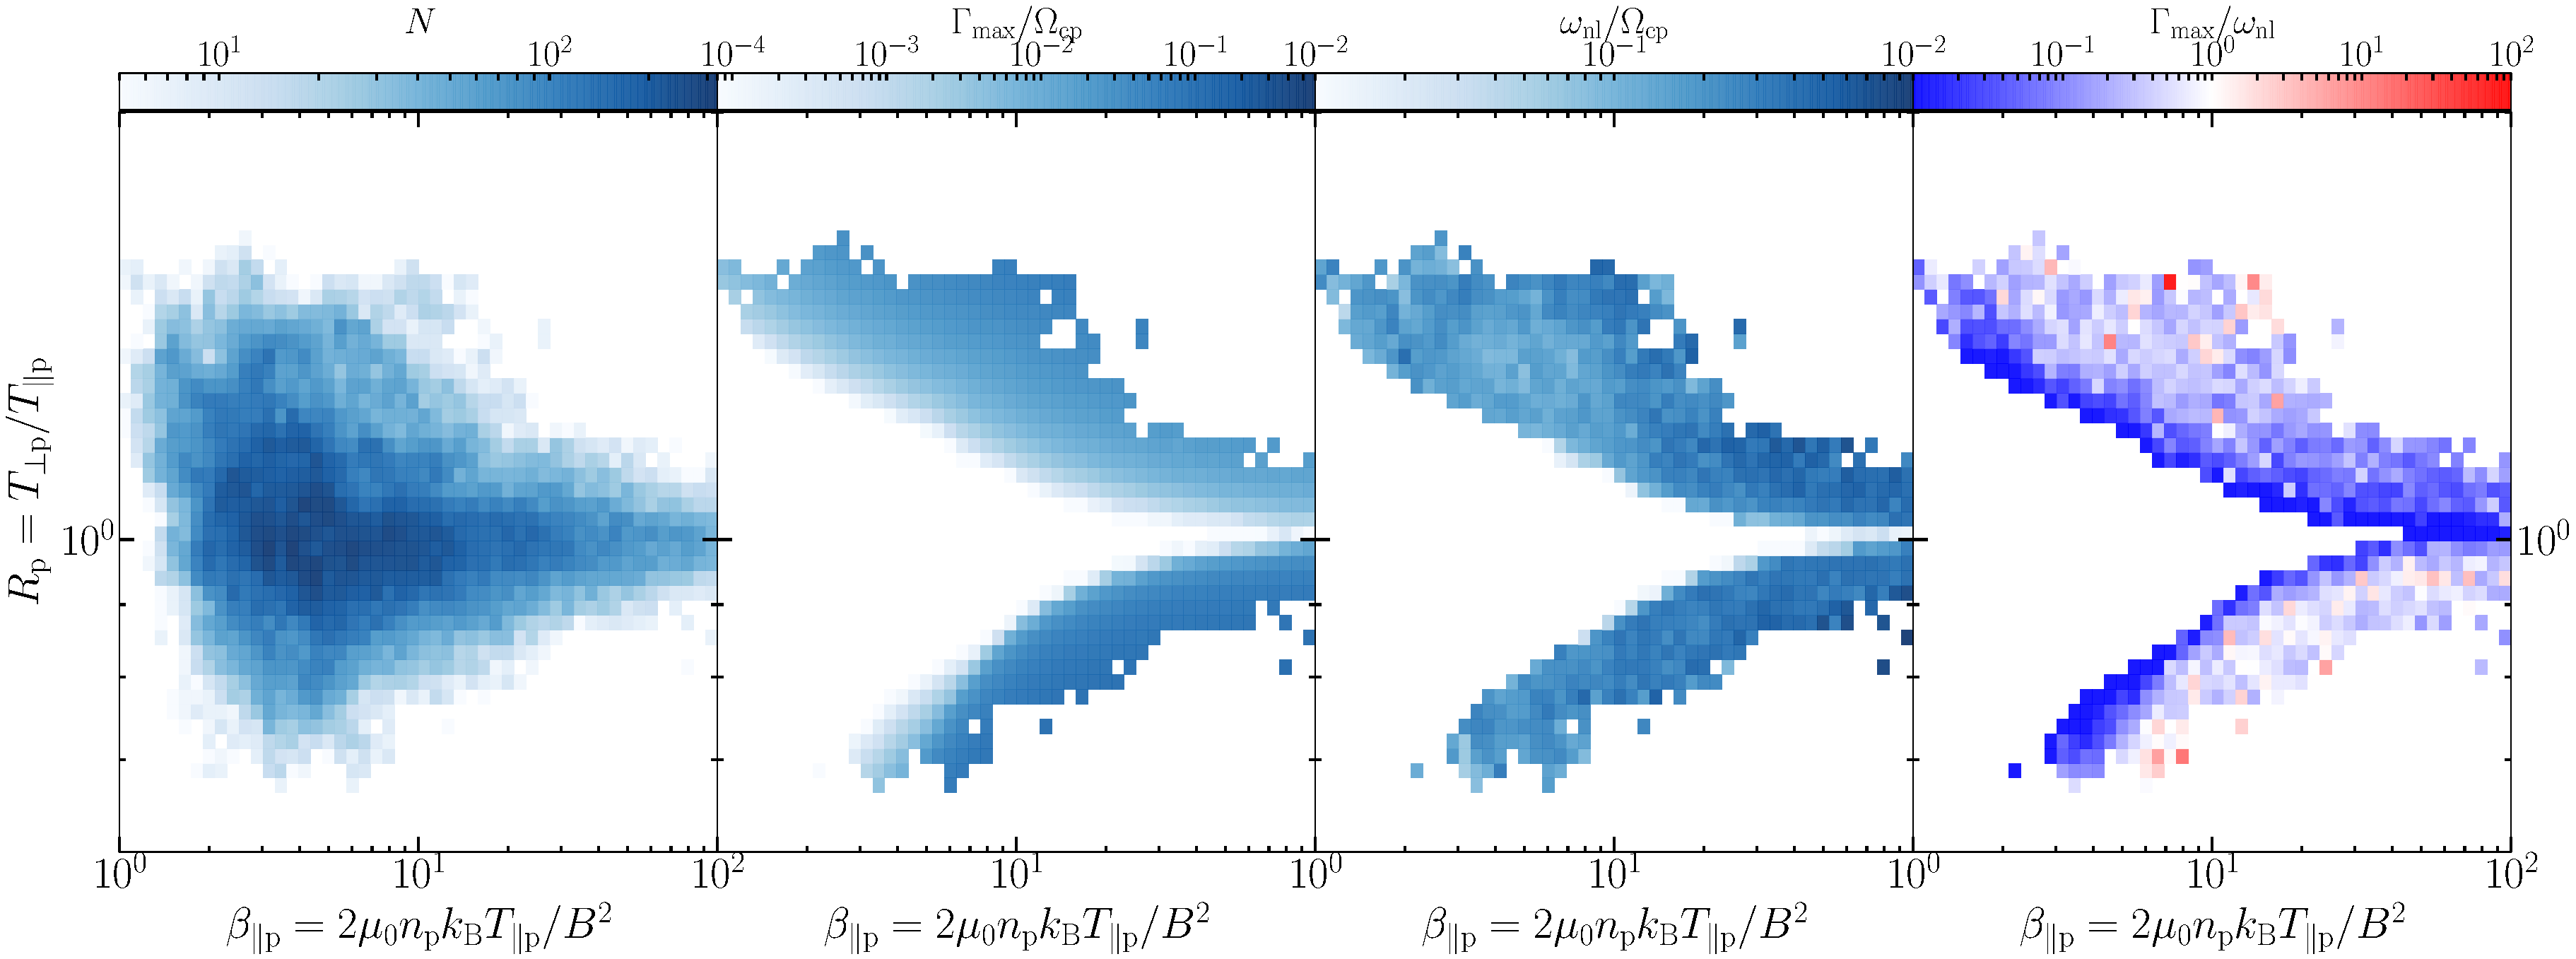
\includegraphics[width=1.\textwidth]{figures/chap7/mms_brz_omega_gamma_mean.pdf}
                    \caption[$(R_{\rm p}, \beta_{\parallel \rm p})$-plot of $\Gamma_{\max}$,
                    $\omega_{\rm nl}$ and $\Gamma_{\max}/\omega_{\rm nl}$ for \texttt{mms}
                    dataset]{$(R_{\rm p}, \beta_{\parallel \rm p})$ plots (from left to right) of
                    distribution of data, maximum linear growth rate ($\Gamma_{\max}$), nonlinear
                    frequency ($\omega_{\rm nl}$), and their ratio ($\Gamma_{\max}/\omega_{\rm nl}$)
                    for earth's magnetosheath.}
                    \label{fig:ratio_brz_mms}
                \end{center}
            \end{sidewaysfigure}

        \begin{sidewaysfigure}
            \begin{center}
                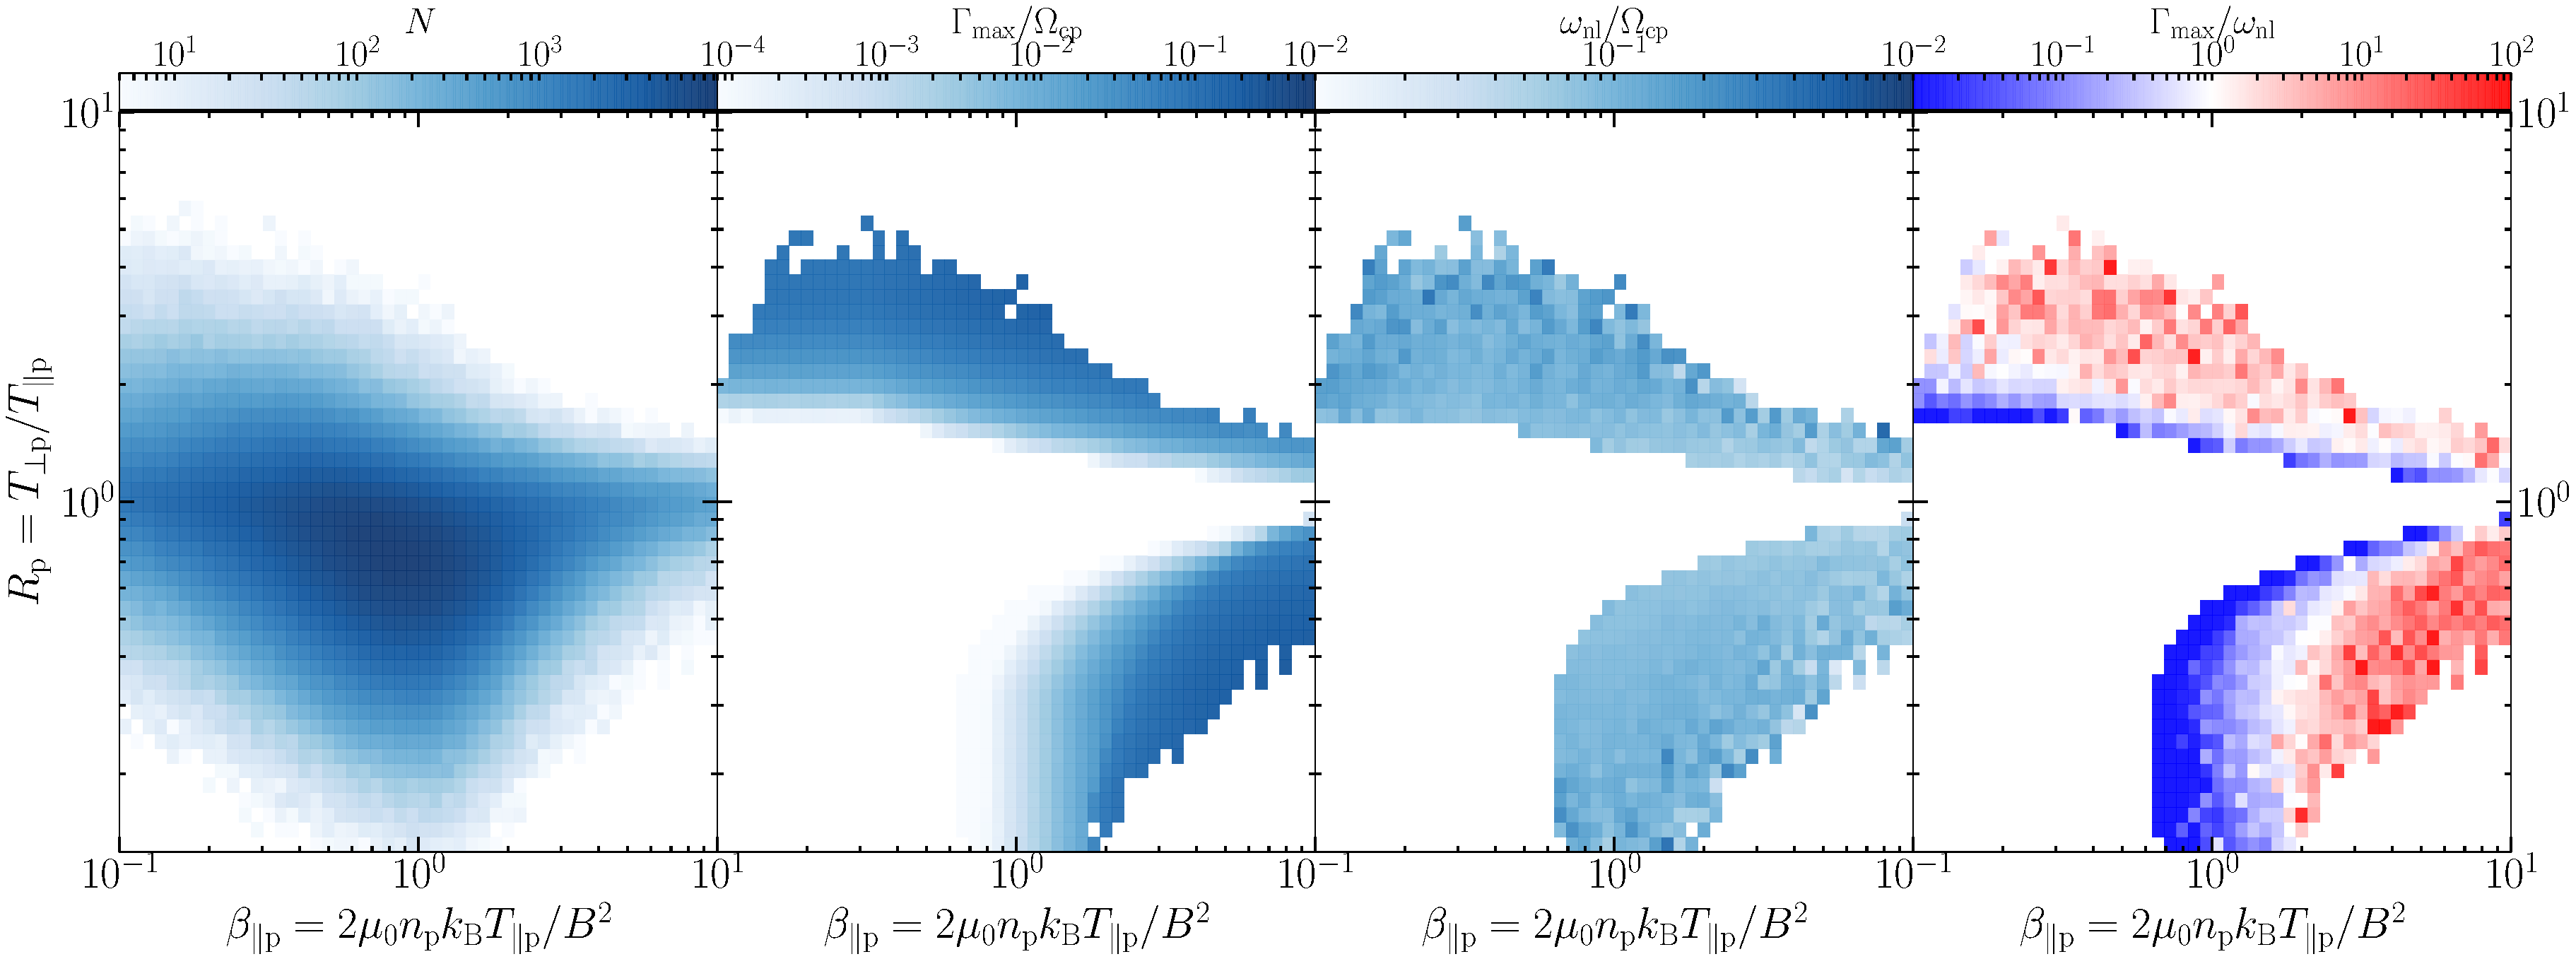
\includegraphics[width=1.\textwidth]{figures/chap7/wnd_brz_omega_gamma_mean.pdf}
                \caption[$(R_{\rm p}, \beta_{\parallel \rm p})$-plot of $\Gamma_{\max}$,
                $\omega_{\rm nl}$ and $\Gamma_{\max}/\omega_{\rm nl}$ for \texttt{wnd}
                dataset]{$(R_{\rm p}, \beta_{\parallel \rm p})$ plots (from left to right) of
                distribution of data, maximum linear growth rate ($\Gamma_{\max}$), nonlinear
                frequency ($\omega_{\rm nl}$), and their ratio ($\Gamma_{\max}/\omega_{\rm nl}$) for
                solar wind at 1-au.}
                \label{fig:ratio_brz_wnd}
            \end{center}
        \end{sidewaysfigure}

        \begin{sidewaysfigure}
            \begin{center}
                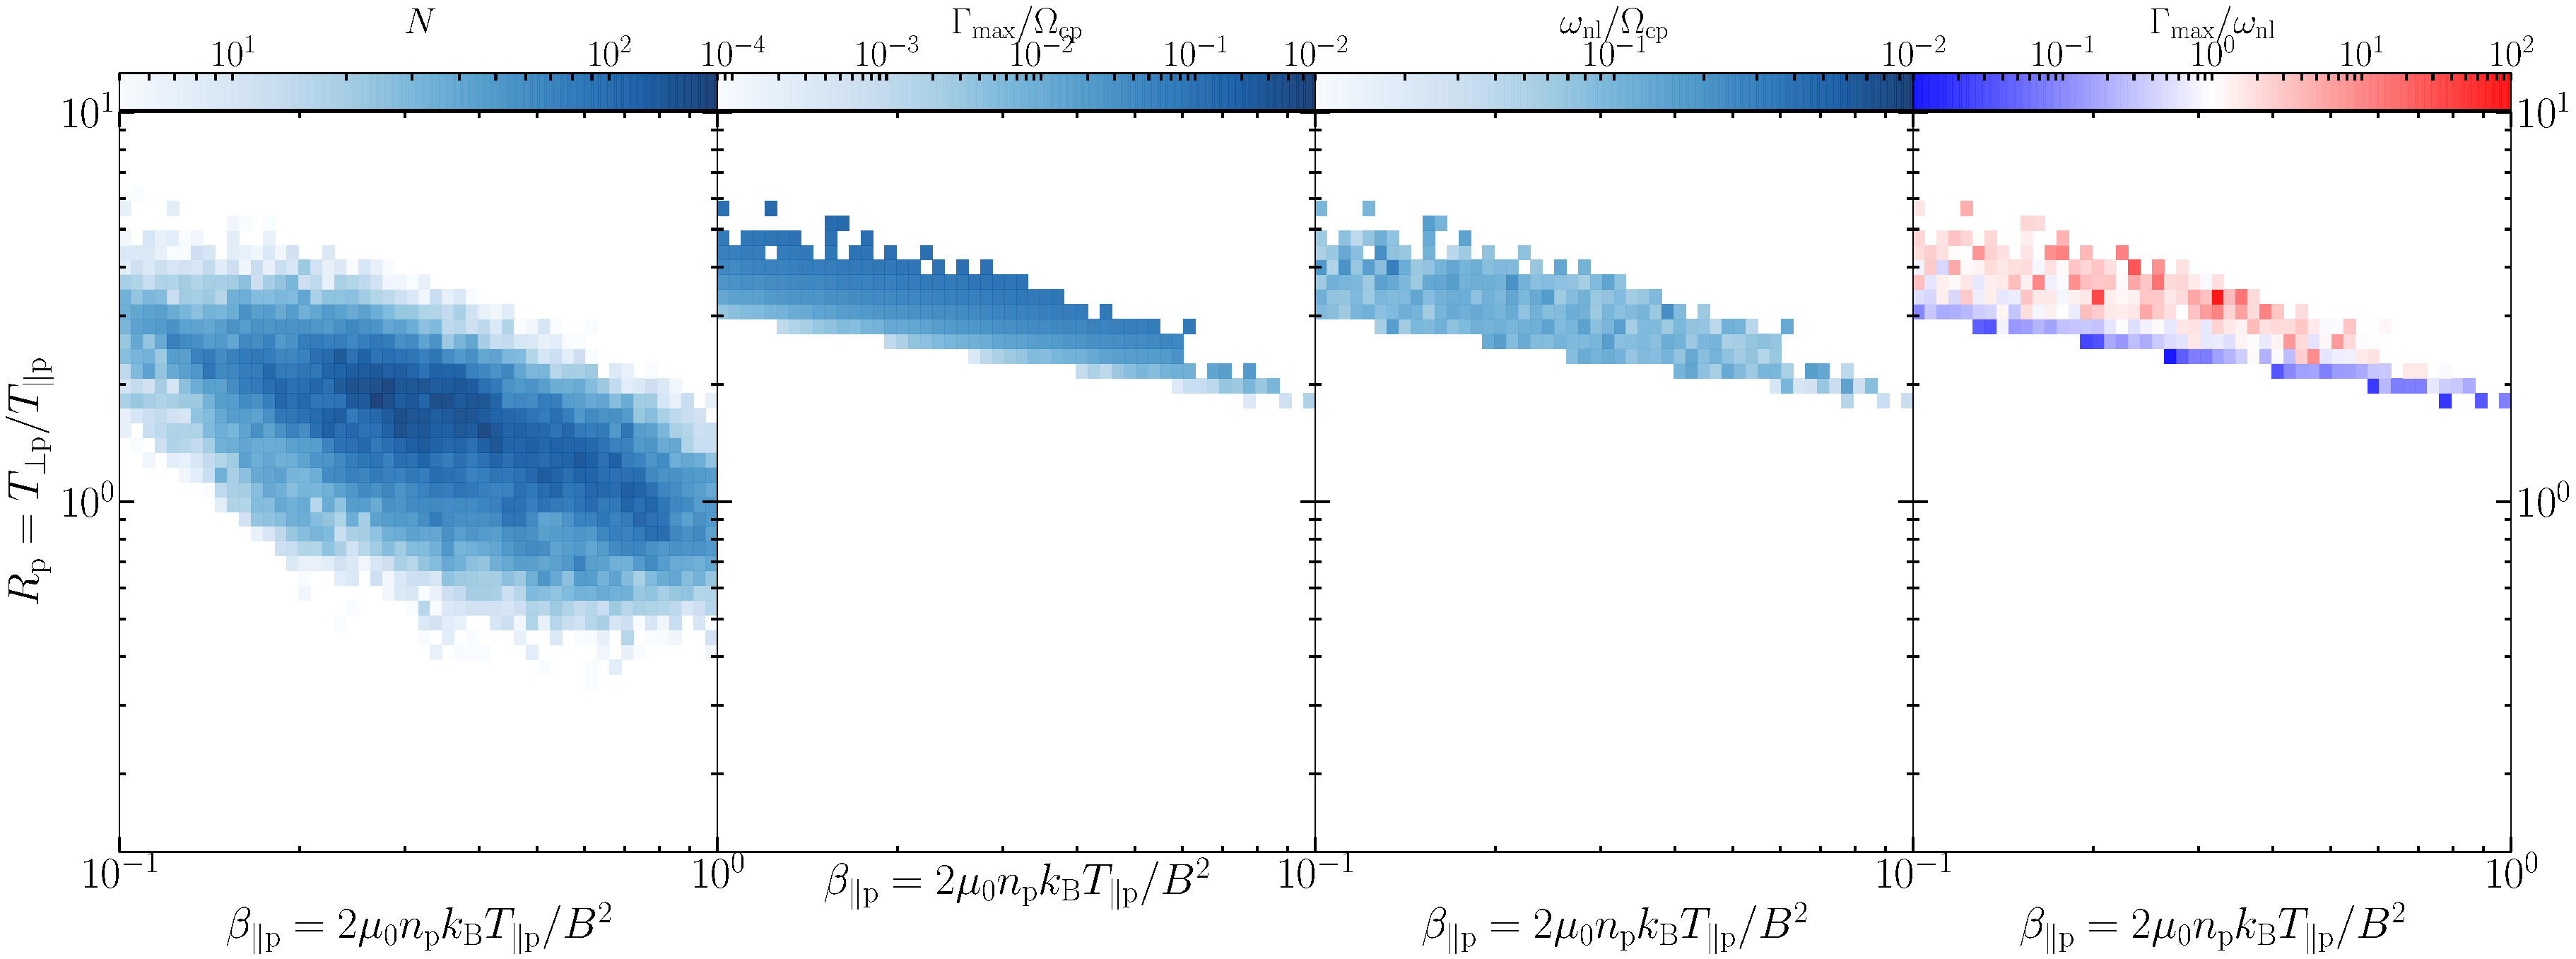
\includegraphics[width=1.\textwidth]{figures/chap7/psp_brz_omega_gamma_mean.pdf}
                \caption[$(R_{\rm p}, \beta_{\parallel \rm p})$-plot of $\Gamma_{\max}$,
                $\omega_{\rm nl}$ and $\Gamma_{\max}/\omega_{\rm nl}$ for \texttt{psp}
                dataset]{$(R_{\rm p}, \beta_{\parallel \rm p})$ plots (from left to right) of
                distribution of data, maximum linear growth rate ($\Gamma_{\max}$), nonlinear
                frequency ($\omega_{\rm nl}$), and their ratio ($\Gamma_{\max}/\omega_{\rm nl}$) for
                solar wind close to the Sun.}
                \label{fig:ratio_brz_psp}
            \end{center}
        \end{sidewaysfigure}

    \section{Discussions} \label{sec:conc7}

        We investigated the competition between linear and non-linear time scales for 6 different
        datasets. We observed that non-linear processes arising because of turbulence dominate
        linear ones overwhelmingly (\Crefrange{fig:ratio_allsim}{fig:ratio_psp}). This would imply
        that the linear processes are of little consequence as far as dynamics and statistical
        properties of a turbulent plasmas is concerned. Yet, in-situ observations of space plasmas
        present strong evidence that linear microinstabilities regulate ion temperature anisotropy.
        Multiple studies of in-situ observations
        \citep{Gary1991,Gary1994,Gary2001,Gary2006,Kasper2002,Hellinger2006,Maruca2011,Maruca2012,Maruca2018},
        have found that the distribution of plasma over the ($R_{\rm p}, \beta_{\parallel \rm p}$)
        plane well restricted by thresholds predicted by linear Vlasov theory\index{Vlasov} one must conclude that
        linear theory works. Observations made in \Crefrange{fig:ratio_brz_mms}{fig:ratio_brz_psp}
        provide further evidence. We observed that though $\omega_{\rm nl} > \Gamma_{\max}$ for most
        part, along the lines of threshold where microkinetic instabilities are most active, linear
        processes disrupt the turbulence cascade and dominate. However, as we saw in
        \Cref{fig:ratio_brz_mms} even when the two processes have comparable values along the edges,
        it still gave rise to expected $(R_{\rm p}, \beta_{\parallel \rm p})$ plot
        \citep{Maruca2018}. Recent studies have shown that regions of extreme temperature anisotropy
        are produced because of generation of sharp gradients by turbulence
        \citep{Osman2011,Greco2012,Valentini2014,Parashar2016}, and we know that kinetic
        microinstabilities are most active where $R_{\rm p}$ deviates significantly from unity.
        \citet{Osman2013} showed that turbulence cascade rates are highest along the edges as well.
        All this indicates a complicated interplay between turbulent and microkinetic phenomena.

        In this chapter we compared linear growth rates derived using linear dispersion relation
        under the assumption of homogeneity of background fields. An ideal method would involve
        computation of $\gamma$ based on theory which takes such inhomogeneities as are present in
        plasmas into account. Understanding the kind of turbulence present in the system can further
        assist us in an accurate computation of $\omega_{\rm nl}$. Since it is extremely difficult
        to gauge the kind of turbulence present in a system without the knowledge of magnetic
        structure a full 3-D image of magnetic field can help substantially. Though development of
        linear theory based on inhomogeneities has been deferred to future work, in
        \Cref{chap:chap8} we discuss a probable future mission and proof of concept for measuring
        full 3-D structure of magnetic field from kinetic to mesoscales at 1\,au.    % This file (chap7.tex) contains the text
                   % for Chapter 7.

%
% This is Chapter 8 file (chap8.tex)
%
\chapter{Magnetic Field Topology Reconstruction Using Machine Learning Algorithm} \label{chap:chap8}

    \section{Overview} \label{sec:ovrvw8}

        Machine learning\index{Machine Learning}, over the last decade has become increasingly relevant in data and image
        analysis. Both, image reconstruction and data imputation, specifically in a time series,
        have increasingly relied on machine learning techniques and algorithm \citep{Wang2018,
        Bertsimas2017}. In this chapter we apply one such algorithm/technique to a synthetically
        generated time series dataset of the magnetic field derived from a fully kinetic 3-D
        simulation of space plasma. This work serves as a proof of concept for a future mission
        consisting of multiple spacecraft that would map out the topology of the solar-wind's
        magnetic field.

        \Cref{sec:intr8} motivates the multi-spacecraft observation of space plasmas and the
        reconstruction of 3-D magnetic field structure. \Cref{sec:bgnd8} presents the current state
        of the field. Synthetic data generation is discussed in \Cref{sec:data8} and
        \Cref{sec:meth8} discusses the methodology used in detail. \Cref{sec:diss8} presents the
        results of the implemented algorithm. The conclusion of the study is summarized in
        \Cref{sec:conc8} along with some discussion and suggestions of future works\footnote{Part of
        this study was published in \citet{Maruca2021}.}.

    \section{Introduction} \label{sec:intr8}

        Over the last 7 decades in-situ observation of solar wind has been carried by different
        spacecraft starting with Sputnik in 1957 and on going with the most recent mission Solar
        Orbiter which was launched in 2020. Majority of such missions launched a single spacecraft.
        Observations from these missions have vastly improved and enhanced our understanding of
        solar wind and its dynamics, thanks to ever increasing, more precise and detailed
        observations. However, single spacecraft missions cannot differentiate between a temporal
        and spatial fluctuation. This also means we do not have detailed information of the full 3-D
        structure of the interplanetary magnetic field. To address this, a few missions have flown
        with 4 or 5 spacecraft (e.g.,
        \discolorlinks{\href{http://www.esa.int/Science_Exploration/Space_Science/Cluster_overview2}{Cluster}},
        \discolorlinks{\href{https://www.nasa.gov/themis-and-artemis}{THEMIS-ARTEMIS}}, and
        \discolorlinks{\href{https://www.nasa.gov/mission_pages/mms/overview/index.html}{MMS}}), and
        missions with even more spacecraft have been proposed \citep{Klein2019a}. Though work done
        by \citet{Fu2015} and \citet{Torbert2020} using MMS data are promising, they are limited to
        a single scale. Methodology employed by \citet{Fu2015} also becomes inaccurate if the
        distance between spacecraft is of the order of ion-inertial length ($d_{\rm i}$). Given the
        multi-scale nature of solar wind \citep{Verscharen2019} we must have a system where we can
        study the magnetic field by reconstructing it at multiple scales. So far no mission has
        succeeded in generating a full three dimensional image of the magnetic vector field in the
        solar wind, mostly because of large number of spacecraft required to carry out such a task
        and at various length scales. A full 3-D image would provide magnetic field vector at every
        point within the area being imaged and thus will be able to trace the interplanetary
        magnetic field lines. It will also get us information related to structure and topology,
        which are extremely important for understanding turbulence and its evolution in space
        plasmas, especially how energy is stored in and transported through the plasma.

        Though an active field of research, not much work has been done in this from the vantage
        point of machine learning. In this study we present a proof of concept of magnetic field’s
        topology reconstruction using multi-point observation in a 3-D simulation box. For
        multi-point observation, we fly a constellation of virtual spacecraft through a simulation
        box (see \Cref{sec:data8}), and carry out the interpolation on observed vector data in the
        3-D space along its trajectory using Gaussian Processes Regression in machine learning. The
        study also explores the number of spacecraft, the relative separation between them, and
        their configuration required for resolving structures of various scales.

    \section{Background} \label{sec:bgnd8}

        Spacecraft make regular in-situ measurement as plasma convects over them. Reconstructing the
        full 3-D topology of interplanetary magnetic field thus requires interpolating the data from
        the finite set of spacecraft observations. Different interpolation techniques can be used to
        achieve this result. Since solar wind is multi-scale in nature \citep{Verscharen2019} we
        will need sufficiently large number of observations to reliably construct the magnetic field
        at various different scales. For a planar configuration of a constellation of spacecraft
        where normal to the plane of orientation is in parallel (or anti-parallel) to the solar wind
        direction, as employed in this study (see \Cref{sec:data8} and \Cref{fig:spc_conf}), we can
        make more observations in the parallel flow direction by increasing the cadence of measuring
        instrument, whereas in the direction perpendicular to the flow, same effect can be achieved
        by increasing the number of spacecraft.
        
        For interpolation between the observation points, because of the presence of non-linear
        structures (see \Cref{chap:chap5}) and sharp discontinuities (see \Cref{chap:chap6}), linear
        interpolation techniques might not be best suited. We thus turn to machine learning
        algorithms in an effort to minimize the number of spacecraft needed and maximize the
        feasibility of such a space mission. Several such machine learning methods for the purpose
        of data imputation have been explored in literature \citep{Lin2019, Bertsimas2017,
        Wang2018}. As discussed in \citet{Lin2019}, the best solution or the most appropriate method
        depends largely on the domain of the problem. What works for one kind of dataset might
        completely fail for a slightly different one, as we will see in this study as well. For our
        purpose, we decided to explore GP and develop an algorithm based on it. The rest of this
        section gives a brief description of GP, some of its salient features, and its key
        advantages and disadvantages.

        \subsection{Gaussian Processes Regression} \label{sec:gpr}

            Gaussian Processes\index{Machine Learning!Gaussian Processes} (GP) as a generic term means that a dataset with finite number of
            observation is modelled as if it were a multivariate normal distribution
            \citep{Gramacy2020}. It is a probability distribution over possible functions that fit a
            given finite dataset. Just as a Gaussian distribution is fully characterised by its mean
            ($\mu$)~and covariance~($\Sigma$), a GP is completely defined by (1) a mean function
            $m(x)$ indicating the mean at any point of the input space and (2) a covariance function
            $K(x,x')$ that sets the covariance between input pairs \textbf{x} and \textbf{x}$'$
            \citep{Rasmussen2006}. These can be written as:
            \begin{align}
                \begin{split}
                    m(\mathbf{x}) & = \mathbb{E}[f(\mathbf{x})] \\
                    k(\mathbf{x},\mathbf{x}') & = \mathbb{E}[(f(\mathbf{x})- m(\mathbf{x}))(f(\mathbf{x}')- m(\mathbf{x}'))] \label{eq:gpr_mx_kx}
                \end{split}
            \end{align}
            and Gaussian processes can be written as:
            \begin{align}
                 f(\mathbf{x}) & \sim \mathcal{GP}\left(m(\mathbf{x}), k(\mathbf{x}, \mathbf{x}')\right) \label{eq:gpr_gp}
            \end{align}
            The covariance matrices in \Cref{eq:gpr_mx_kx} can be computed using a predefined
            function, which are referred as kernels in GP. This sets a prior to the set of functions
            which must be considered for a given dataset and the type of kernel chosen defines the
            characteristics of this prior.

            There are several standard kernels (see \Cref{sec:meth8}). For this study, we tried a
            few which were available through one the Python packages and selected the one most
            suitable for our dataset.

            One of the advantages of using GP in this application is that it is non-parametric and
            thus, doesn't require a priory fit function to model the input data. It is particularly
            relevant to our case since we do not have much information about the structure of the
            solar wind. Rather than relying on fit function, GP look at every possible model and
            probabilistically explore the space to find the most optimal one for a given dataset.
            Naively, it will appear that there are infinite functions to be considered here since
            the probabilistic approach used in GP considers all possible functions. In reality, this
            is not the case since each function is assigned a prior and the infinite number of
            functions are defined by their statistics, making the whole method a lot more
            manageable. Another advantage of GP is its computational tractability
            \citep{Rasmussen2006}.
            
            Selection of an appropriate kernel, though important to the whole process is not
            critical, as even if we choose a random kernel it often does a decent job of data
            imputation.  Recent development in Deep GP in fact do away with the issue of
            pre-defining a kernel since it is designed to learn the kernel which works best for a
            given dataset \citep{Bui2016}. Well calibrated predictive uncertainty estimates and ease
            of generalization, for both regression and classification analyses, are other benefits
            of using GP.

            As with any method, there are some disadvantages associated with it. One of the major
            drawback of GP is its computational cost. Since inversion of matrices is required, which
            makes the method of $\mathcal{O}(n^3)$, it is computationally very expensive to run for
            large number of data points (n~$>$~2000) \citep{Gramacy2020}.

    \section{Kernels in Gaussian Processes} \label{sec:meth8}

        For this study we implemented GP using
        \discolorlinks{\href{https://scikit-learn.org/stable/index.html}{SciKit Learn}} package
        available in Python \citep{Pedregosa2011}. SciKit has a few default kernels\index{Machine Learning!kernels} implemented in
        the package, we list out some of them here:

        \begin{enumerate}[]
            \item Constant Kernel (CK)
            \item Radial-basis Function Kernel (RBF)
            \item Mat\'ern Kernel (MK)
            \item Rational Quadratic Kernel (RQ)
            \item Exponential-Sine-Squared Kernel (ESS)
        \end{enumerate}
        For our study we used these five kernels either individually or in combination with each
        other. We briefly discuss each of the aforementioned kernels here. A more in-depth
        discussion of each kernel can be found in \citet{Rasmussen2006} or on the
        \discolorlinks{\href{https://scikit-learn.org/stable/modules/gaussian_process.html\#kernels-for-gaussian-processes}{SciKit
        Learn}}
        web-page\footnote{https://scikit-learn.org/stable/modules/gaussian\_process.html\#kernels-for-gaussian-processes}.\\
        \\
        \textbf{1.\,Constant Kernel\index{Machine Learning!kernels!constant}}: By definition this is simply a constant number or a vector for
        all points in the space. This is largely useful in combination with other kernels where
        either modification of magnitude (Product kernel) or change of mean (Sum kernel) is
        required. The kernel can be written as:
        \begin{align}
            \begin{split}
                k(x_{\rm i},x_{\rm j}) & = constant\_value \;\forall\; x_{\rm i}, x_{\rm j} \label{eq:cst_ker}
            \end{split}
        \end{align}
        \\
        \textbf{2.\,Radial-basis Function kernel\index{Machine Learning!kernels!RBF}}: The RBF kernel is also known as ``squared
        exponential kernel". The kernel has one length parameter `$l$' which can be set to either a
        scalar or something which has same dimension as the input ($x_{\rm i}$). The length
        parameter controls the smoothness of the kernel. The kernel is stationary, meaning its
        covariance function is invariant under translation, and it is infinitely differentiable
        resulting in smooth outputs. The kernel is given as follows:
        \begin{align}
            \begin{split}
                k(x_{\rm i}, x_{\rm j}) & = \exp\left(- \frac{d(x_{\rm i}, x_{\rm j})^2}{2l^2} \right) \label{eq:rbf_ker}
            \end{split}
        \end{align}
        where $d(x_{\rm i}, x_{\rm j})$ is the Euclidean distance between the two points.\\
        \\
        \textbf{3.\,Mat\'ern Kernel\index{Machine Learning!kernels!Mat\'ern}}: Mat\'ern kernel is the generalized form of RBF with an
        additional parameter `$\nu$' which controls the smoothness of the resulting function. As
        $\nu \rightarrow \infty$, Mat\'ern kernel approaches RBF. Generally since `$\nu$' is set to
        some finite value, the resulting output may not be very smooth. However, it gives a mode to
        control the smoothness of the output. The Mat\'ern kernel is given as:
        \begin{align}
            \begin{split}
                k(x_{\rm i}, x_{\rm j}) & = \frac{1}{\Gamma(\nu)2^{\nu-1}}\left(\frac{\sqrt{2\nu}}{l} d(x_{\rm i} , x_{\rm j})\right)^\nu K_\nu\left(\frac{\sqrt{2\nu}}{l} d(x_{\rm i} , x_{\rm j} )\right) \label{eq:mat_ker}
            \end{split}
        \end{align}
        where $K_{\nu}(\cdot)$ is a modified Bessel function and $\Gamma(\cdot)$ is the gamma
        function. For most cases we set `nu' to 3/2 or 5/2 for once or twice differentiability
        respectively.\\
        \\
        \textbf{4.\,Rational Quadratic Kernel\index{Machine Learning!kernels!RQ}}: The kernel is an infinite sum of RBF with various
        length scales. Just like RBF, RQ has the `$l$' parameter. It also has an additional
        parameter `$\alpha$' which is the scale mixture parameter. The kernel can be written as:
        \begin{align}
            \begin{split}
                k(x_{\rm i}, x_{\rm j}) & = \exp\left(- \frac{d(x_{\rm i}, x_{\rm j})^2}{2\alpha l^2} \right)^{-\,\alpha} \label{eq:raq_ker}
            \end{split}
        \end{align}
        \\
        \textbf{5. Exponential-Sine-Squared Kernel\index{Machine Learning!kernels!exponential sine squared}}: The kernel has two parameters, length scale
        `$l$' and periodicity `$p$' consequently making it most suitable for modelling functions
        with some kind of periodic nature. The kernel can be written as:
        \begin{align}
            \begin{split}
                k(x_{\rm i}, x_{\rm j}) & = \exp\left(- \frac{2~sin^2(\pi d(x_{\rm i},x_{\rm j})/p)}{l^2} \right) \label{eq:ess_ker}
            \end{split}
        \end{align}

        For our purpose, we mostly used kernels in combination with each other, since most kernels
        can be added or multiplied to others. After Using several kernels, we observed that a
        combination of constant and Mat\'ern kernels gave the best result for circular
        configuration, as shown in \Cref{fig:spc_conf}, whereas for grid-like distribution (see
        \Cref{fig:gpr_cas_bx}) of spacecraft we found that constant and RQ kernels gave the best
        result. Thus, the final kernel used to obtain results reported in this study were:\\


        \vspace{-1em}
        \begin{itemize}
            \item For a grid-like configuration,
            \begin{align}
                \begin{split}
                    {\rm kernel}_{\blacksquare} = {\rm CK}(2, (10^{-2}, 10^{2})) + {\rm CK}(2, (10^{-2}, 10^{2})) \cdot      {\rm RQ}(l=2, \alpha=0.1) \label{eq:fin_ker_grd}
                \end{split}
            \end{align}
            \item For a circular configuration,
            \begin{align}
                \begin{split}
                    {\rm kernel}_{~\Newdot} = {\rm CK}(5, (10^{-2}, 10^{2})) + {\rm CK}(5, (10^{-2}, 10^{2}))\cdot {\rm        MK}(l= [2,2,6], \nu=5/2) \label{eq:fin_ker_cir}
                \end{split}
            \end{align}
        \end{itemize}


        Where the symbols have the same meaning as defined for \Crefrange{eq:cst_ker}{eq:ess_ker}.

    \section{Synthetic Data Generation} \label{sec:data8}

        For implementing the GP as discussed in \Cref{sec:gpr}, we would need observation dataset
        from a constellation of spacecraft. However, since we do not have such a constellation we
        use the output from a fully kinetic 3-D simulation, \texttt{ros} (see \Cref{sec:3pic} for
        more details). This enables us to test the effect of various number of spacecraft and their
        relative orientation and positioning on the quality of reconstructed image. For the ease of
        computation we down-sampled the original data to have resolution of 1\,$d_{\rm i}$ in the
        $xy$-plane and $\sim$\,1/3\,$d_{\rm i}$ along the $z$-axis. To generate synthetic data from
        the simulation data, we flew constellations of different number of spacecraft (4 to 36) in
        different configurations through the simulation box. \Cref{fig:spc_conf} shows one such
        configuration (radial and planar) for 24 spacecraft. Note that all 24 spacecraft are in one
        plane and record the time series as plasma passes by at typical solar wind speed
        ($\sim$\,500\,km/s). We simulate the observation at a cadence of $\sim$\,13\,Hz which is
        comparable to modern instruments (see \Cref{chap:chap4}). Under the assumption of Taylor's
        hypothesis \citep{Taylor1938}, which lets us convert from a time scale to length scale using
        the speed of the plasma, solar-wind speed corresponds to consecutive data points separated
        by approximately $0.3\,d_{\rm i}$ along the $z$-axis. This spacing is small compared to
        distance between spacecraft ($2 - 22\,d_{\rm i}$) and thus reconstruction along $z$-axis is
        limited by the cadence of observation, whereas along $xy$-plane the number of spacecraft
        limits the resolution.
        \begin{figure}
            \begin{center}
                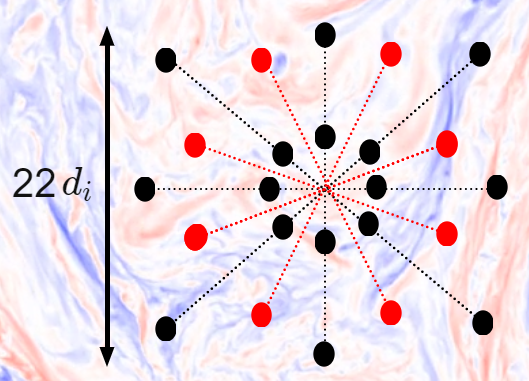
\includegraphics[width=1.\textwidth]{figures/chap8/spc_config_24.png}
                \caption[Configuration for 24 spacecraft]{One of the many configuration of
                spacecraft for 24 spacecraft. The inner black circles represent spacecraft at a
                distance of 2 $d_{\rm i}$ from the center whereas the outer ones are at 11 $d_{\rm
                i}$. The red dots are the spacecraft at 7 $d_{\rm i}$ from the center.}
                \label{fig:spc_conf}
            \end{center}
        \end{figure}

    \section{Methodology} \label{sec:method8}

        Simulation box size is $41.9\,d_{\rm i}$, and thus it takes the constellation roughly 10
        seconds to cross the whole box and each spacecraft makes 128 measurement in one flight. We
        use the synthetic time series data generated from the virtual spacecraft trajectory to train
        our GP model (see \Cref{sec:meth8} and \Cref{apdx:C}). If we have $N$ spacecraft in a given
        configuration and we have 128 observation along the $z$-axis. For one configuration we get
        $128 \times N$ data points for each component of the magnetic field to train our model. Once
        the training is complete, we feed in the coordinates of every point inside the disk of size
        28\,$d_{\rm i}$ (a few $d_{\rm i}$'s larger than the size of the constellation) for all the
        different planes, a total of 128 planes. This means for any number of spacecraft we must
        make predictions at $\sim 28 \times 28 \times 128$ points. This implies that greater number
        of spacecraft in any given configuration will give us better result since it will increase
        the amount of data used to train the model. However, as with any machine learning algorithm,
        there is a limit to how well trained a given model can be no matter the amount of input
        data. We discuss this in further detail in next section.

        Once we have the time series data, we trained the specified model on the observed data
        providing it one component at a time. Once the model is trained and the parameters of the
        model are learned based on the training set, we provide the model with all the locations in
        3-D space where we need to find the value of magnetic field. \Cref{apdx:C} gives the detail
        of implementation and also provide the code for the same.
    
    \section{Results} \label{sec:diss8}

        \Crefrange{fig:gpr_cas_bx}{fig:gpr_cas_bm} show one of the slice along xy-plane of the
        actual simulation data in Panel (\textbf{a}) (down sampled to 1\,$d_{\rm i}$ resolution) and
        the reconstructed field corresponding to different number of spacecraft employed (4 to 36,
        represented by the black dots) for observation (Panels \textbf{b} to \textbf{f}). For these
        figures, as discussed in \Cref{sec:meth8} reconstructed field were generated using kernel as
        defined in \Cref{eq:fin_ker_grd}. The configurations with 4 and 9 spacecraft poorly
        reproduce the original simulated field. Only when we have at least 16 spacecraft some
        structure is captured. Only for a constellation of 25 or more spacecraft does the
        reconstructed field closely resemble the original field structure. Though there is slight
        improvement in how well the original field is being captured when we  from 25 to 36
        spacecraft (as expected), whether this is worth additional expense of adding 11 more
        spacecraft need further investigation and a quantitative comparison.

        \begin{figure}
            \begin{center}
                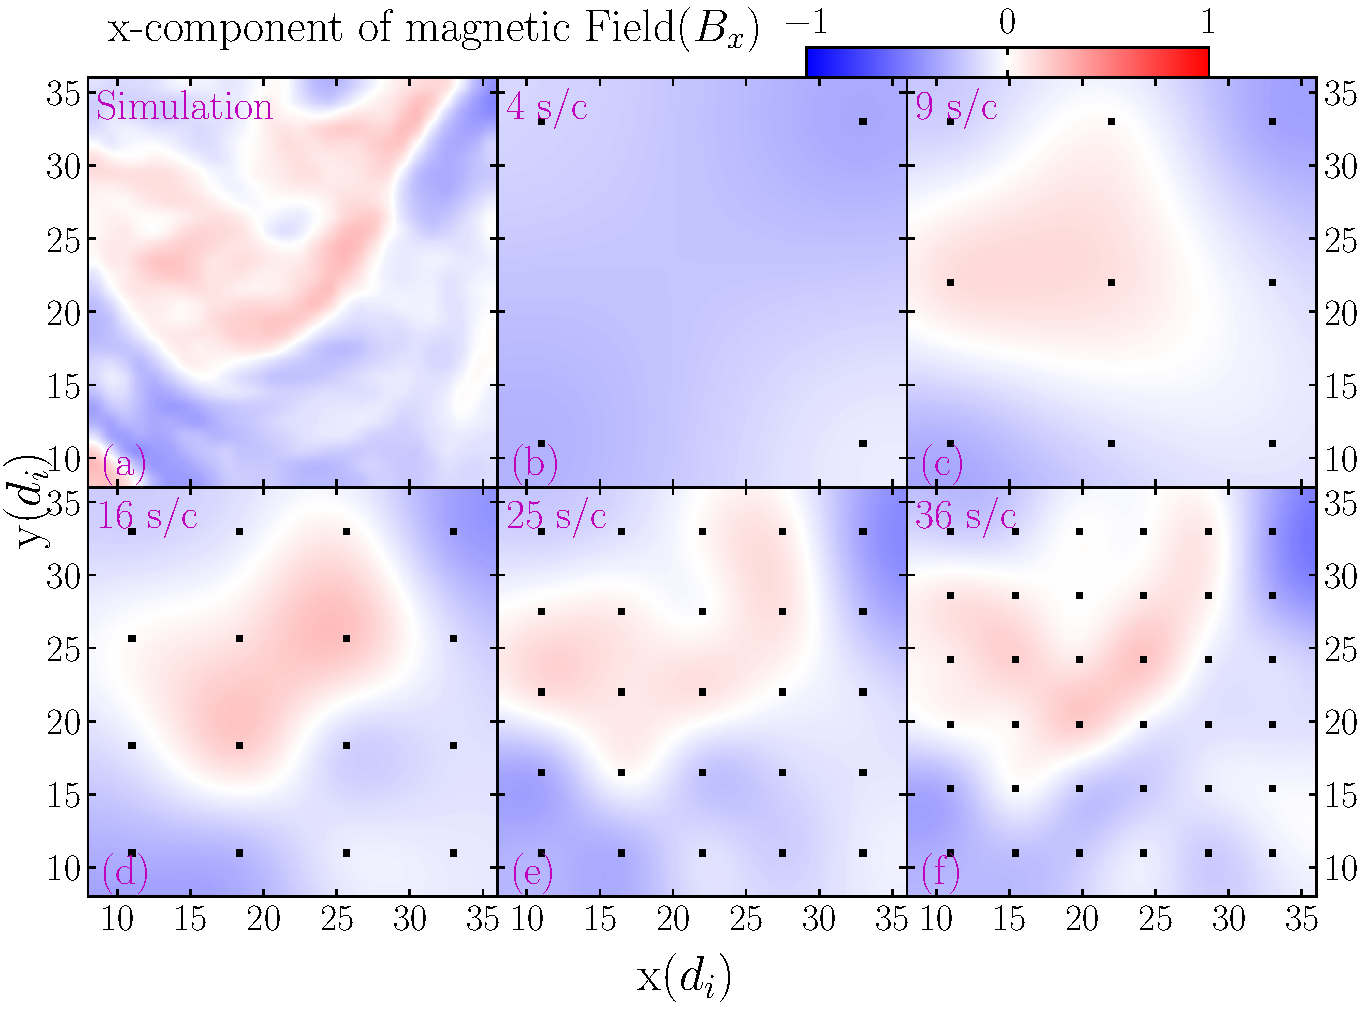
\includegraphics[width=0.85\textwidth, height=3.65in]{figures/chap8/all_spc_bx_4_9_16_25_36_001_cas1.pdf}
                \caption[Reconstructed field (x-component), linear configuration]{x-component of
                magnetic field from simulation (Panel \textbf{a}) and reconstructed field
                corresponding to different number of spacecraft (Panels \textbf{b} to \textbf{f})}
                \label{fig:gpr_cas_bx}
            \end{center}
        \end{figure}

        \begin{figure}
            \begin{center}
                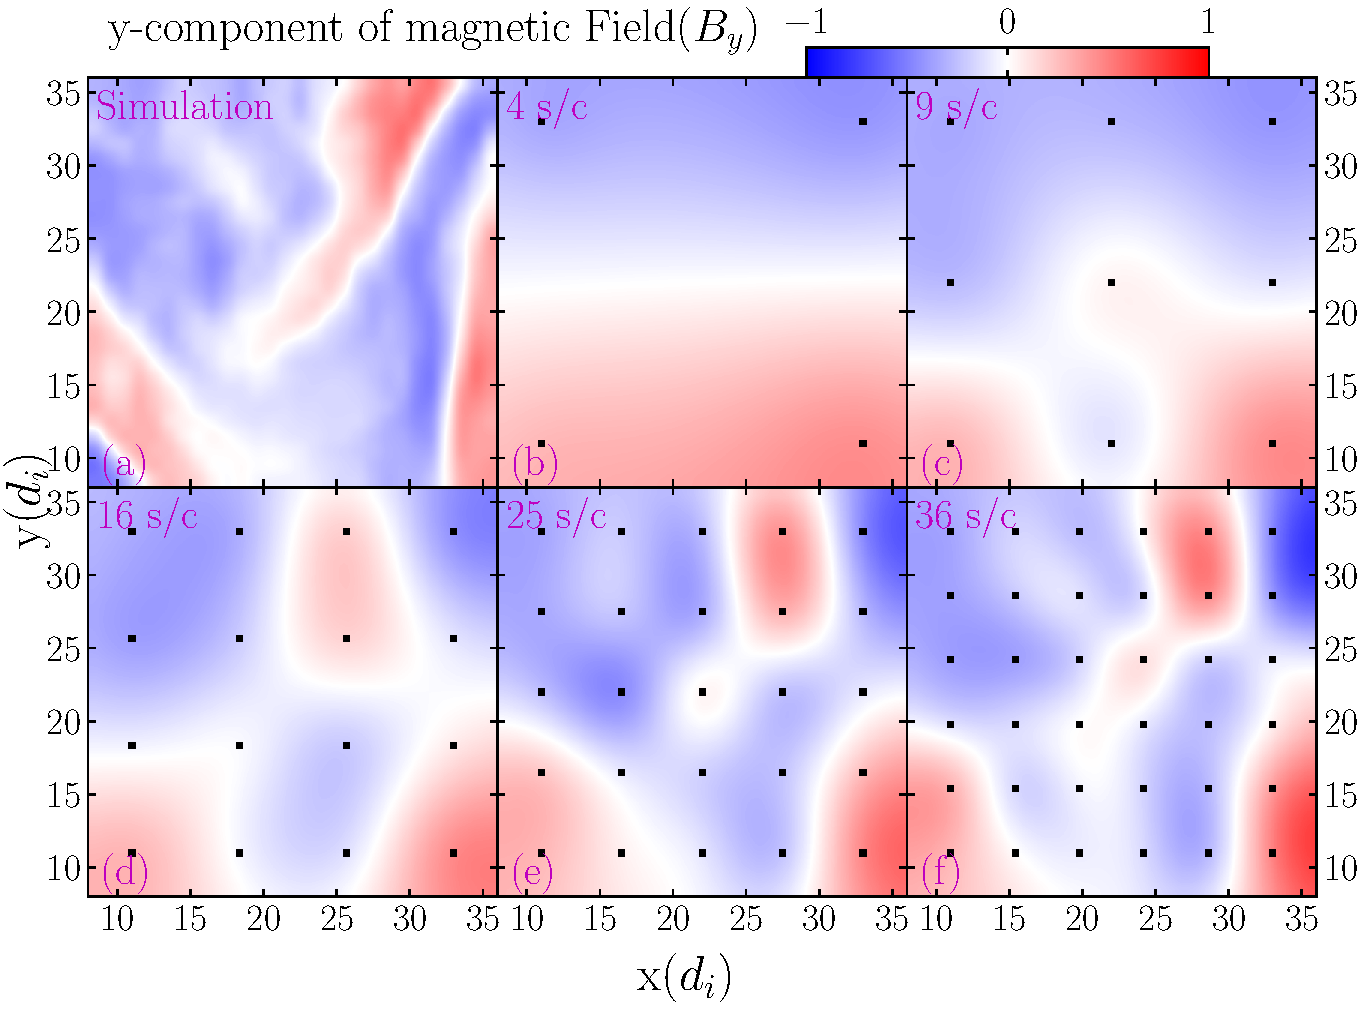
\includegraphics[width=0.85\textwidth, height=3.65in]{figures/chap8/all_spc_by_4_9_16_25_36_001_cas1.pdf}
                \caption[Reconstructed field (y-component), linear configuration]{y-component of
                magnetic field from simulation (Panel \textbf{a}) and reconstructed field
                corresponding to different number of spacecraft (Panels \textbf{b} to \textbf{f})}
                \label{fig:gpr_cas_by}
            \end{center}
        \end{figure}

        \begin{figure}
            \begin{center}
                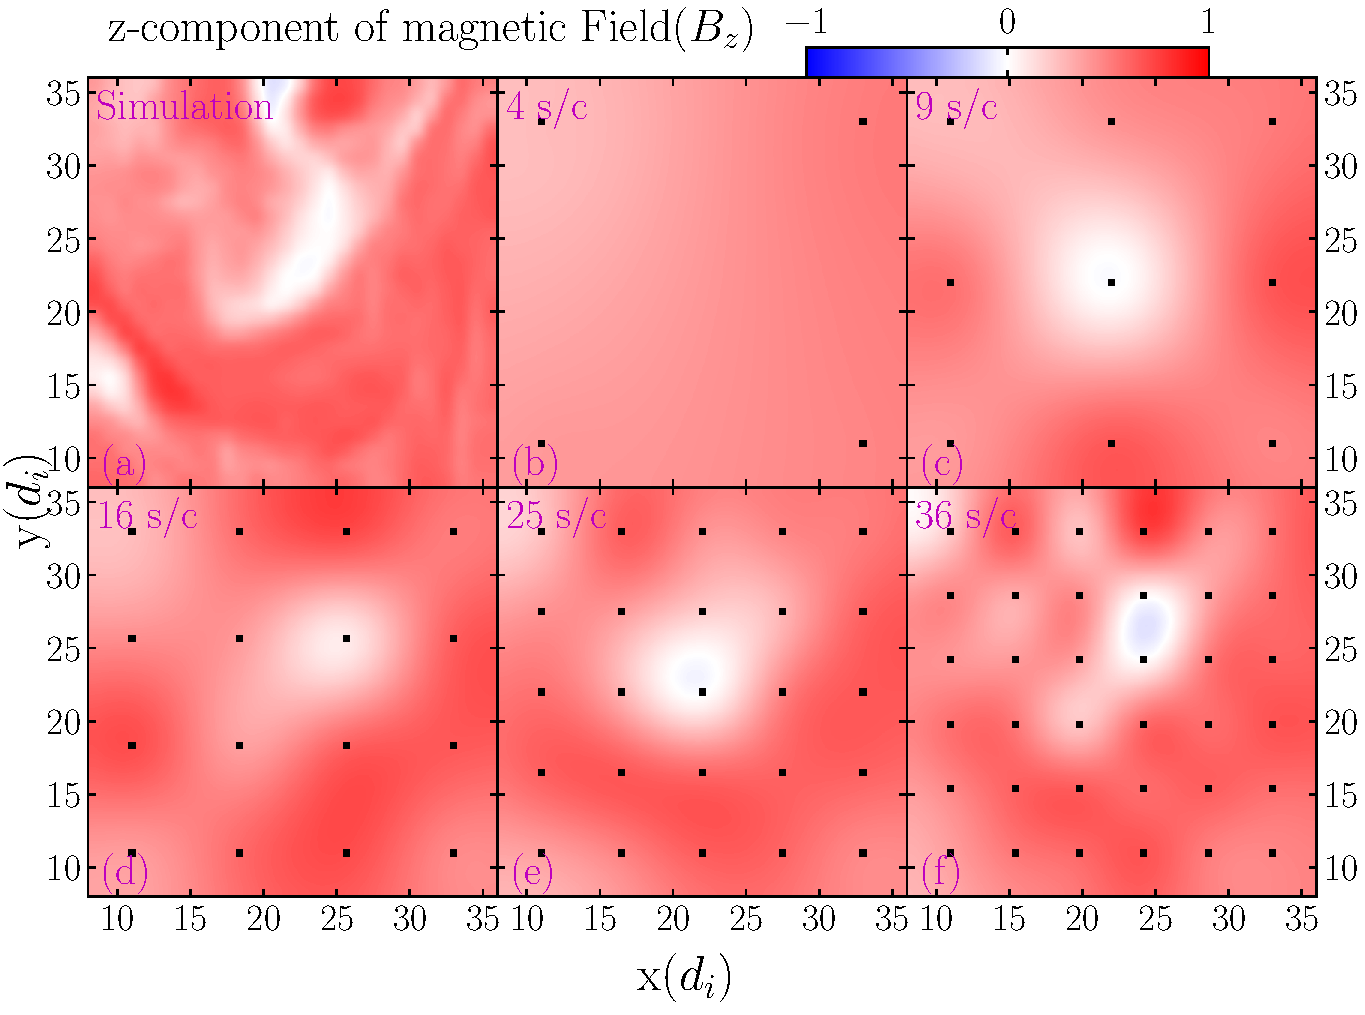
\includegraphics[width=0.85\textwidth, height=3.65in]{figures/chap8/all_spc_bz_4_9_16_25_36_001_cas1.pdf}
                \caption[Reconstructed field (z-component), linear configuration]{z-component of
                magnetic field from simulation (Panel \textbf{a}) and reconstructed field
                corresponding to different number of spacecraft (Panels \textbf{b} to \textbf{f})}
                \label{fig:gpr_cas_bz}
            \end{center}
        \end{figure}

        \begin{figure}
            \begin{center}
                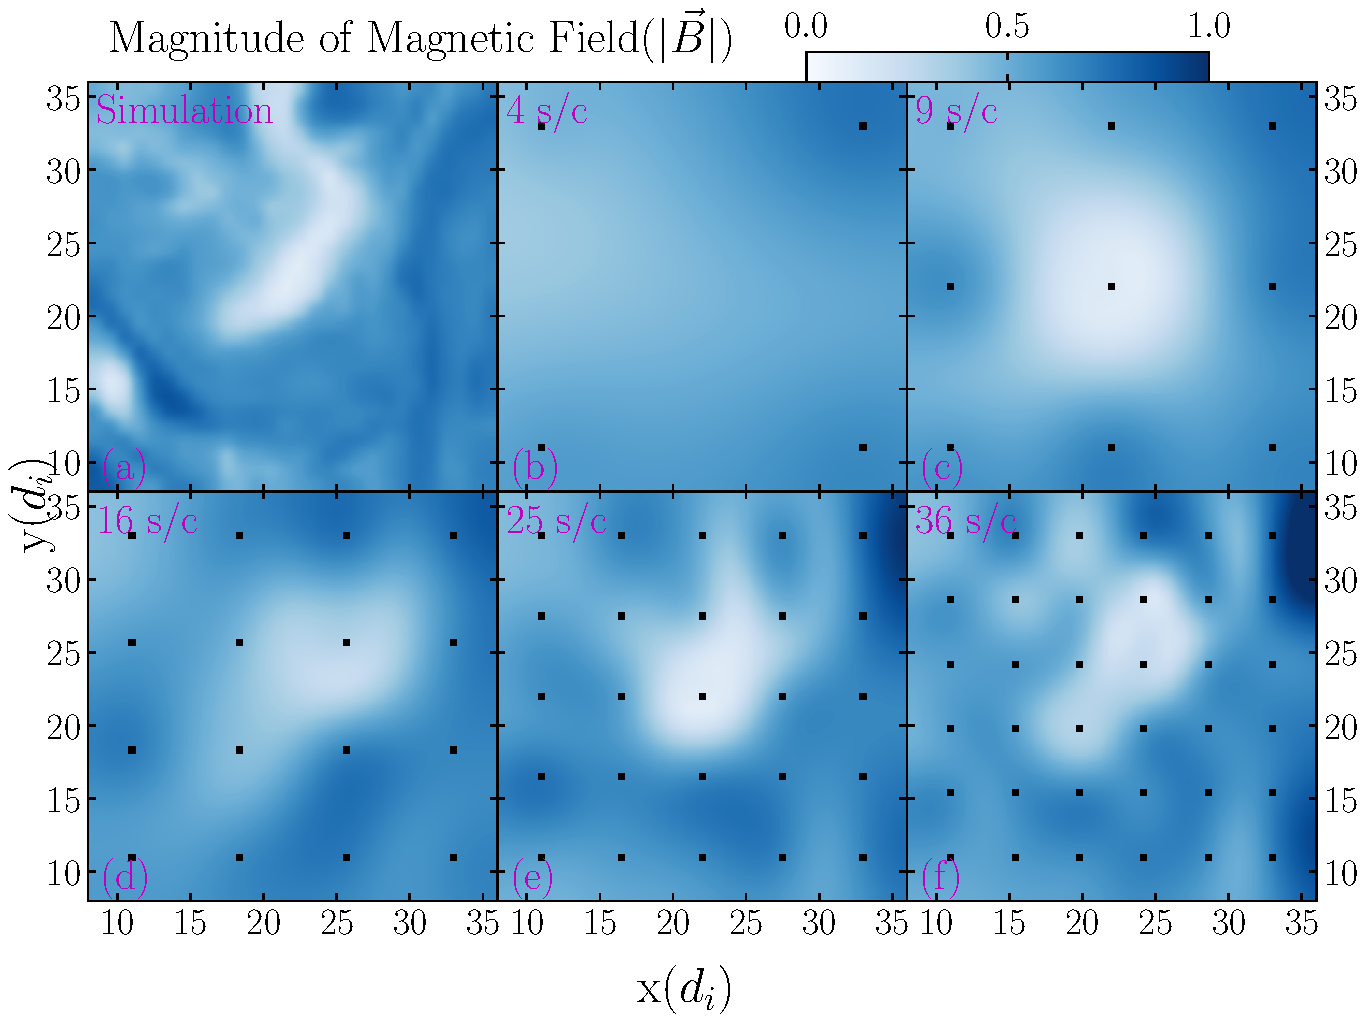
\includegraphics[width=0.85\textwidth, height=3.65in]{figures/chap8/all_spc_bm_4_9_16_25_36_001_cas1.pdf}
                \caption[Reconstructed field, linear configuration]{Magnitude of magnetic field from
                simulation (Panel \textbf{a}) and reconstructed field corresponding to different
                number of spacecraft (Panels \textbf{b} to \textbf{f})}
                \label{fig:gpr_cas_bm}
            \end{center}
        \end{figure}

        Results from circular configurations of spacecraft, for which the kernel in
        \Cref{eq:fin_ker_cir} was used, are shown in \Crefrange{fig:gpr_bx}{fig:gpr_bm}. As
        discussed for the previous figures, Panel (\textbf{a}) shows the original data, whereas
        Panels (\textbf{b}) to (\textbf{h}) show reconstructed field corresponding to different
        number of spacecraft. The spacecraft are distributed around a common center such that
        irrespective of the number of spacecraft employed, maximum distance between two spacecraft
        is always 22$\,d_{\rm i}$ so that they all cover equal volume of space in any given amount
        of time. As was the case for grid-like configuration, reconstructed fields do not capture
        any meaningful structure for 4 or 8 spacecraft. Some structure does show up for 16
        spacecraft however it is only when we employ 24 or more spacecraft that we get the structure
        of the field which looks similar to the original input (more on this later).

        For 24 spacecraft, we also randomized the position of each spacecraft, such that each
        spacecraft could be anywhere in a circle of radius 2$\,d_{\rm i}$ from its starting position
        (see Panel \textbf{g}). Reconstructed data, even for randomized position, continue to
        capture the actual structure of the original field. This observation considerably lessens
        the burden of having precisely defined orbits of each spacecraft. As long as individual
        spacecraft can communicate with each other regarding their relative position, reconstruction
        is not effected in a significant way.

        Given that we have a large number of spacecraft, at least 24, for this observation, a
        scenario might arise where one or more of them fail to function properly, either because of
        partial or full failure of instruments or for any other conceivable reason. We considered
        this scenario in the following way. We record the position of all spacecraft as shown in
        Panel (\textbf{g}) of \Crefrange{fig:gpr_bx}{fig:gpr_bm} and randomly remove two spacecraft,
        as shown in Panel (\textbf{h}) of the same figures. We then carry out GP on the modified
        data. Results from such reconstruction are shown in Panel (\textbf{h}) of each figure. As
        one can see, though the quality of reconstruction deteriorates a bit, compared to 24
        spacecraft (Panel \textbf{e}) it still manages to capture most of the structure present.
        These two observations (randomized location of spacecraft and random failing of 2 out of 24
        spacecraft) shows the robustness of algorithm.

        Based on the results we have shown so far, we thus conclude that if such an algorithm were
        to be applied, we will need at least 24 spacecraft in different configuration.
        \begin{figure}
            \begin{center}
                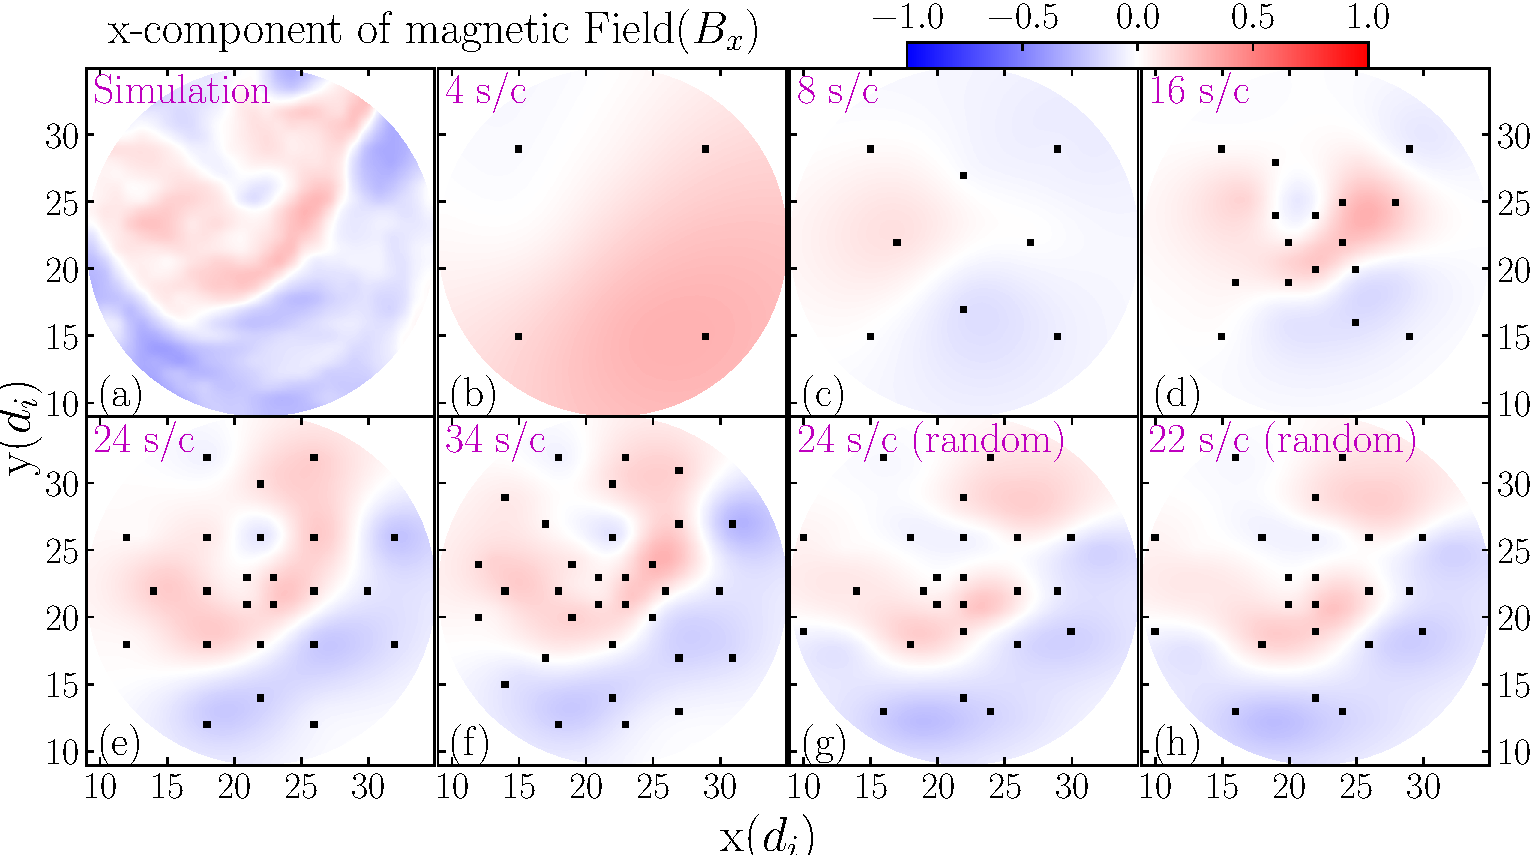
\includegraphics[width=0.85\textwidth]{figures/chap8/all_spc_bx_4_8_16_24_34_24_22_000.pdf}
                \caption[Reconstructed field (x-component), circular configuration]{x-component of the magnetic field from simulation (a) and various different number for circular configuration of spacecraft (b to h)}
                \label{fig:gpr_bx}
            \end{center}
        \end{figure}

        \begin{figure}
            \begin{center}
                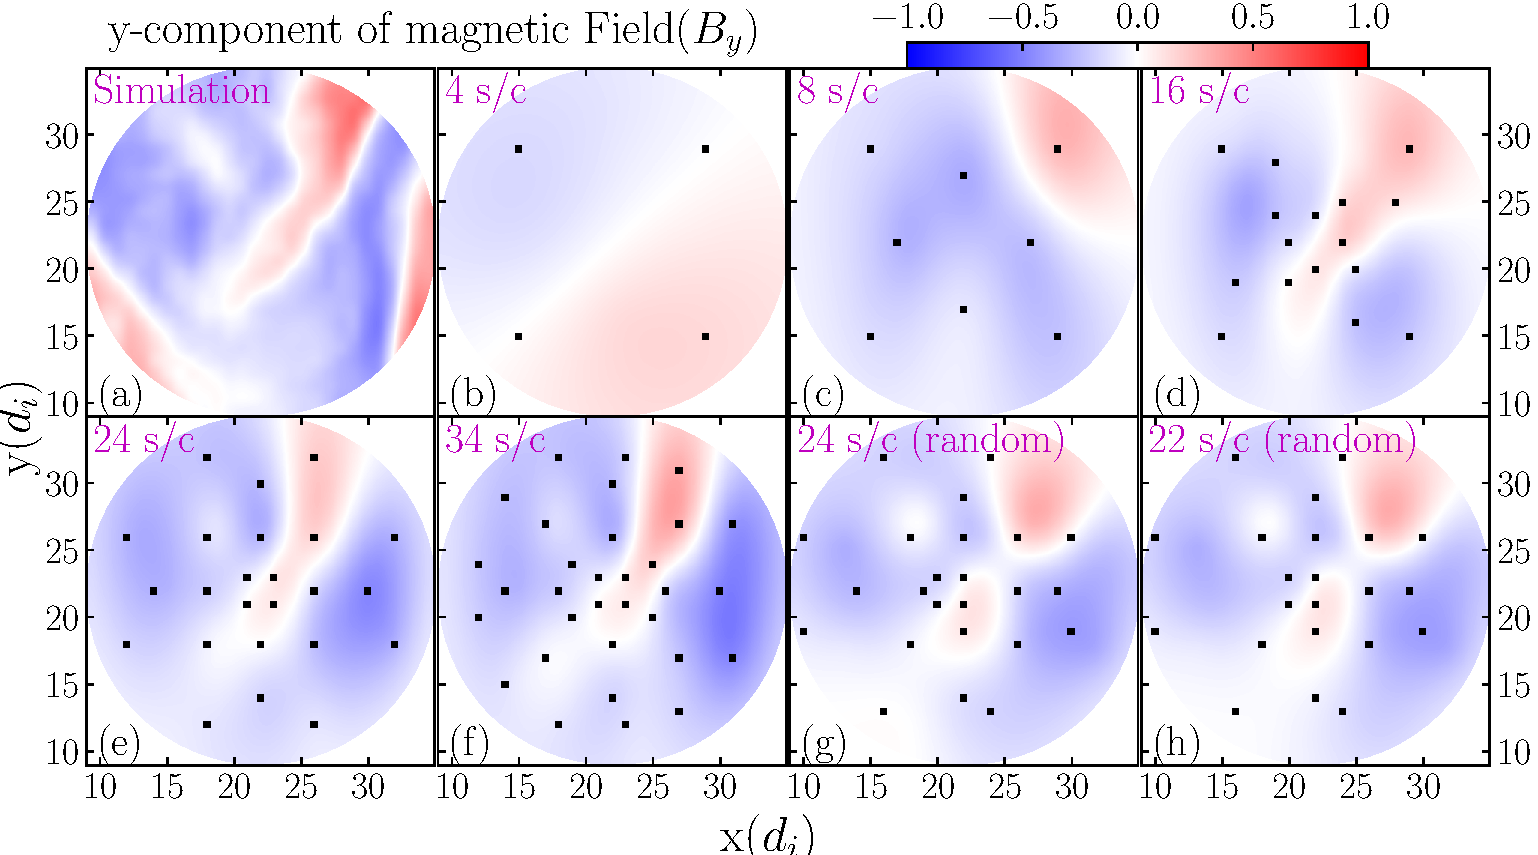
\includegraphics[width=0.85\textwidth]{figures/chap8/all_spc_by_4_8_16_24_34_24_22_000.pdf}
                \caption[Reconstructed field (y-component), circular configuration]{y-component of the magnetic field from simulation (a) and various different number for circular configuration of spacecraft (b to h)}
                \label{fig:gpr_by}
            \end{center}
        \end{figure}

        \begin{figure}
            \begin{center}
                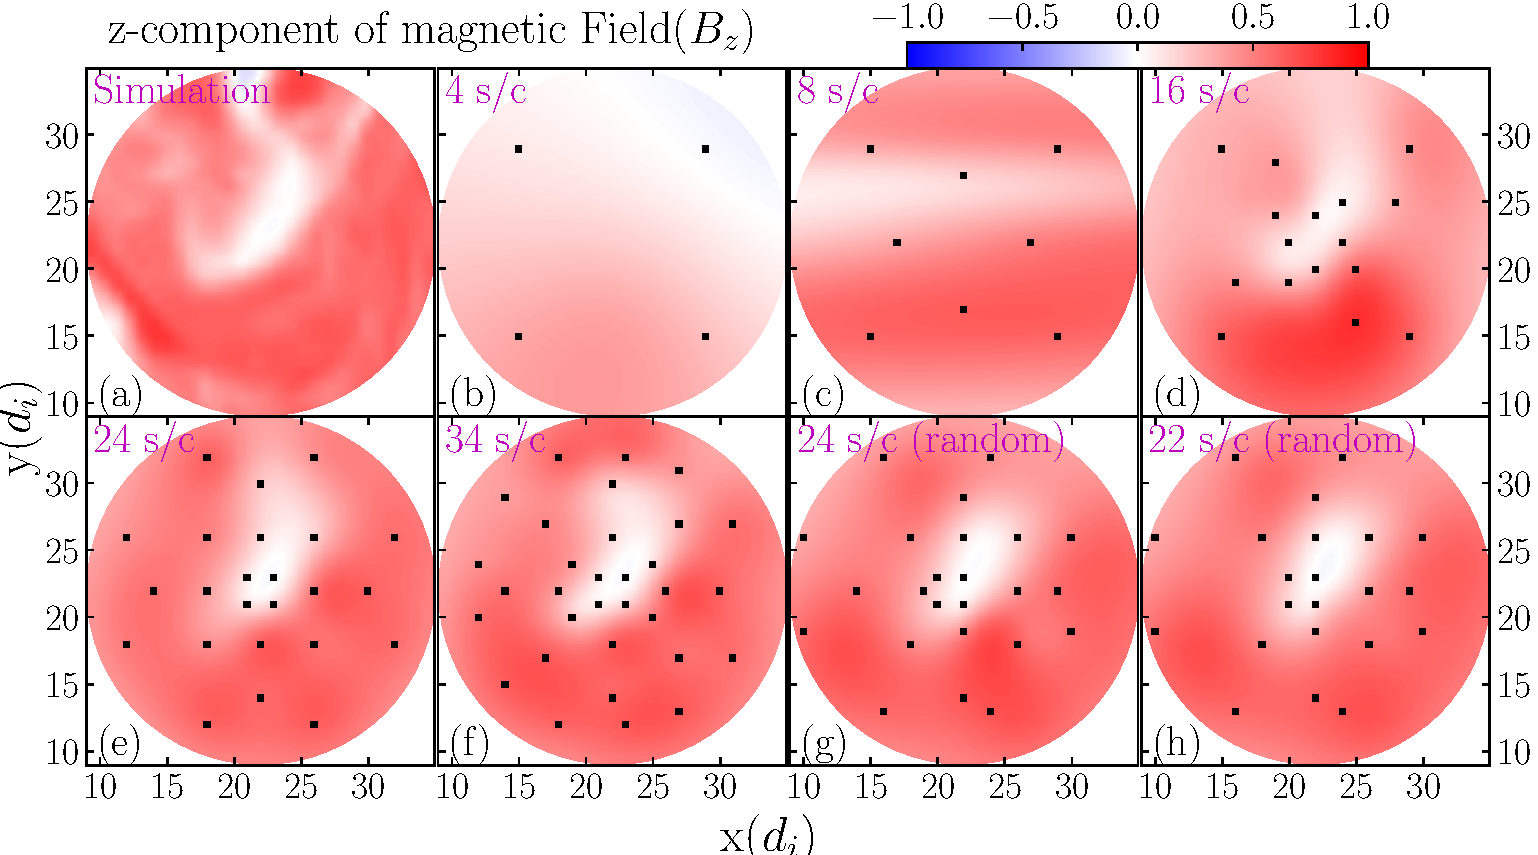
\includegraphics[width=0.85\textwidth]{figures/chap8/all_spc_bz_4_8_16_24_34_24_22_000.pdf}
                \caption[Reconstructed field (z-component), circular configuration]{z-component of the magnetic field from simulation (a) and various different number for circular configuration of spacecraft (b to h)}
                \label{fig:gpr_bz}
            \end{center}
        \end{figure}

        \begin{figure}
            \begin{center}
                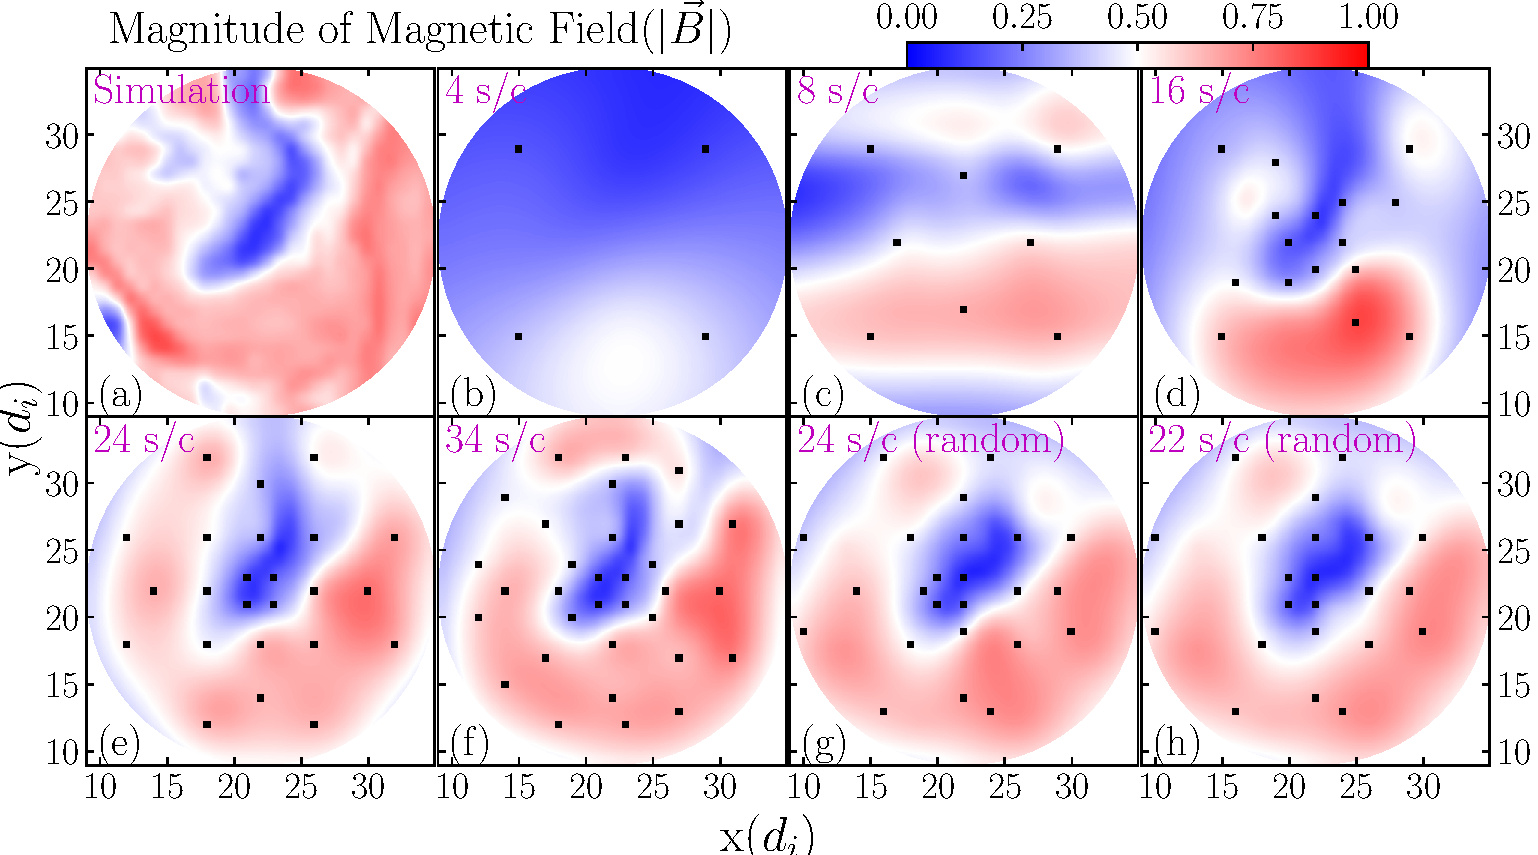
\includegraphics[width=0.85\textwidth]{figures/chap8/all_spc_bm_4_8_16_24_34_24_22_000.pdf}
                \caption[Reconstructed field, circular configuration]{Total magnetic field from simulation (a) and various different number for circular configuration of spacecraft (b to h)}
                \label{fig:gpr_bm}
            \end{center}
        \end{figure}
        
    \section{Discussions} \label{sec:conc8}

        The unknown nature of turbulence in the solar wind has given rise to competing theories to
        explain the structure and evolution of the interplanetary magnetic field and how energy is
        transferred from one scale to another. Measurements from a single spacecraft cannot
        differentiate between temporal and spatial fluctuations in the field and thus cannot
        conclusively support or reject any one of these theories. Measurements of the field's
        complete 3-D morphology and topology will enable us to understand the true nature of
        solar-wind turbulence. This study thus focused on determining the baseline number of
        spacecraft required to produce 3-D images of the IMF from in-situ magnetic field
        measurements.

        Using fully kinetic 3-D PIC simulation data, we demonstrated magnetic field topology
        reconstruction from synthetic time series in 3-D space using Gaussian Processes, a machine
        learning algorithm. Our results indicate that 24 spacecraft would be required for the
        satisfactory reconstruction of 3-D IMF structure. We also showed that precise control of
        spacecraft trajectory is not required for such a mission so long as the spacecraft positions
        are known. A baseline of 24 spacecraft even allows for unfavorable alignment of some
        spacecraft, though substantially fewer spacecraft (e.g., 16) fail to produce consistently
        adequate IMF reconstructions.

        Nevertheless, this study is still very much a work in progress and much needs to be done
        before we can reach a final version of the algorithm. As stated in \Cref{sec:meth8}, we
        applied GP to each component of the field individually, ignoring the other two components.
        In reality the magnetic field components are not fully independent since the magnetic field
        must be divergence-less.  In principle, a kernel could be implemented that would process all
        three components simultaneously and even enforce the requirement of a divergence-less field
        \citep[for a 2-D example of this, see][]{Narcowich2007,Wahlstroem2013}.  Alternatively a
        divergence cleaning algorithm could be applied after the GP algorithm has run. 
        
        We are also investigating alternative machine learning techniques. For example Deep GP
        \citep{Bui2016} can generate the best kernel for a given dataset rather than requiring the
        user to select one.

        More study is also required of how the arrangement of a given number of spacecraft affects
        the accuracy of magnetic reconstruction. A key component of this would be developing
        quantitative metrics for assessing reconstruction quality. A simple point by point
        comparison cannot take into account the benign distortion and blurring which arises because
        of reconstruction using a finite number of spacecraft. Instead, we are focusing on
        physically relevant parameters of magnetic structures: e.g., the connectivity of magnetic
        fields and the aspect ratios and orientations of regions of weak/strong magnetic field.    % This file (chap8.tex) contains the text
                   % for Chapter 8.

\newpage\null\thispagestyle{empty}

%
% This is Chapter 9 file (chap9.tex)
%
\chapter{Conclusion}\label{chap:chap9}

    \section{Broader Context} \label{sec:bcc9}

        Space plasmas such as the solar wind and terrestrial magnetosheath are highly structured and
        dynamic systems. Over the last few decades, two different theoretical frameworks have been
        developed to study their formation and evolution. The first uses linear Vlasov theory to
        explore micro-scale phenomena: the effects of waves and the constraints imposed by
        microinstabilities on the plasmas. The second includes the larger mesoscales and focuses on
        non-linear processes such as turbulence and the coherent structures it generates.

        Though both these frameworks have strong observational supports (see \Cref{sec:app2}), they
        are incompatible as traditionally formulated. Linear theory explicitly assumes a homogeneous
        background for the linear fluctuations that it studies. In contrast, turbulence produces
        strong inhomogeneities at all scales --- including those of linear theory. Reconciling these
        incongruous theories has motivated the work of this thesis.

        We focused our work on ion temperature-anisotropy and heating. Many previous studies have
        identified the heating of solar wind and magnetosheath to be ubiquitous but strongly
        inhomogenous (see \Cref{sec:inter3b}). The rate of heating varies across time and space and
        is often highly anisotropic which leads to strong temperature-anisotropies
        ($T_{\perp}/T_{\parallel} \neq 1$). The observations and simulations strongly indicate that
        turbulence produces inhomogeneous and anisotropic heating (see \Cref{sec:res5,sec:diss6}).
        Likewise, the predicted constraints of linear Vlasov theory align well with the observed
        distribution of ion temperature-anisotropy (see \Cref{sec:app2}). Despite their
        contradictory assumptions, both turbulence and microinstabilities seem to substantially
        affect ion-temperature in space plasmas. We conjectured that though turbulence produces
        inhomogeneities, the plasma remains sufficiently homogeneous at the kinetic micro-scales for
        the fastest modes of linear instability to develop.

    \section{Summary of Key Results} \label{sec:summ9}

        In \Cref{chap:chap5} we reported our analysis on the interplay of temperature-anisotropy
        driven linear microkinetic instabilities and intermittency arising as a consequence of
        turbulence. We showed that the two processes occur in close physical space. We also found
        the indication that the linear instabilities occur in discrete regions or intervals in
        different kinds of simulations as well as in in-situ data from space plasmas (see
        \Crefrange{fig:brjhb}{fig:brjwnd}).

        In \Cref{chap:chap6} we studied how intermittent structures affect the heating of the
        nascent solar wind and the terrestrial magnetosheath.. We used PVI to quantify
        intermittency. Study \citep{Osman2012a} using the same technique at 1\,au shows similar
        result thereby suggesting the ubiquitous nature of PVI heating. While we observed strong
        positive correlation between PVI and radial proton-temperature for the solar wind,
        magnetosheath plasma show little correlation. As discussed in \Cref{sec:diss6} some of the
        reasons for poor correlation might be the lower average value of PVI in magnetosheath as
        compared to the solar wind, small duration of observations as well as the relatively longer
        duration of the PVI events might be other contributing factors. In any case, this remains
        poorly understood and rather surprising given the positive correlation observed between PVI
        and the electron temperature \citep{Chasapis2018}. For the solar wind, we also found
        elevated value of conditionally averaged radial temperature up to one correlation length
        away from the point of a PVI event (see \Cref{fig:tem_pvi_lag}).

        In \Cref{chap:chap7} we compare the characteristic time scales of microinstabilities to
        those of turbulence at the same size scales for 6 different datasets. We observed that for
        the vast majority of data points/regions where the conditions were unstable, turbulence time
        scale is shorter than linear time scale (see
        \Crefrange{fig:ratio_allsim}{fig:ratio_kde_all}). This means that linear instabilities
        rarely have enough time to grow and affect the plasma before turbulence changes the plasma
        conditions driving the instability. However, since anisotropy is well regulated by the
        instability thresholds, we looked at the relative values of two time scales along the edges
        of Brazil plot. We found that along the edges linear instabilities do become faster than
        their turbulence counterpart and thus are able to regulate the extreme values of anisotropy
        (see \Crefrange{fig:ratio_brz_mms}{fig:ratio_brz_wnd}).

        At present we cannot image full structure of the interplanetary magnetic field using a few
        spacecraft. However, constellations with larger and larger number of spacecraft are becoming
        increasingly common with several possible missions to be launched in near future. Thus with
        a view towards the future, we carried out a study in \Cref{chap:chap8} to reconstruct the
        3-D topology and morphology of the interplanetary magnetic field from observations made by
        such a constellation with finite number of spacecraft. Using Gaussian Processes in machine
        learning for different configurations of number and arrangement of spacecraft, we showed
        that we need a baseline of 24 spacecraft to successfully carry out such a process. A
        complete 3-D image of the magnetic field will significantly advance our understanding of
        turbulence in space plasmas and and shed light on the exact process of turbulence cascade.    % This file (chap9.tex) contains the text
                   % for Chapter 9.

\newpage\null\thispagestyle{empty}
\newpage\null\thispagestyle{empty}

%\include{ref}      % This file (ref.tex) contains the text
                   % for the references.

\vspace*{\fill}
\hspace*{0pt}\hfill \Huge{BIBLIOGRAPHY} \hspace*{0pt}\hfill
\vspace*{\fill}
\normalsize
\newpage\null\thispagestyle{empty}

%
% This is the Bibliography file (bibtex.tex)
% This generally works for BibTeX

% Use sample.bib for BibTeX database
\bibliography{bibliographies/Books,bibliographies/Papers}
% BibTeX style (plain, alpha, unsrt, abbrv, apalike, siam, acm, aasjournal, abbrvnat)
\bibliographystyle{aasjournal}
\nocite{}
   % This file (bibtex.tex) contains the text
                   % for a bibliography if using BibTeX with
                   % sample.bib

%\newpage\null\thispagestyle{empty}\newpage

%\include{app}      % This file (app.tex) contains the text
                   % for one Appendix. 

\vspace*{\fill}
\hspace*{0pt}\hfill \Huge{APPENDIX} \hspace*{0pt}\hfill
\vspace*{\fill}
\normalsize
\newpage\null\thispagestyle{empty}\newpage

%
% This is the Appendix A file (appA.tex)
%
\appendix{Brazil Plots} \label{apdx:A}

    In \Cref{sec:app2} we showed Brazil-plots from dataset \texttt{wnd} (\Cref{fig:brazil_prob_wnd})
    and \texttt{mms} (\Cref{fig:brazil_prob_mms}). Here we show the Brazil-plot from rest of the
    datasets mentioned in \Cref{chap:chap4}.
    
    We observe that for 2.5-D simulations because of low values of $R_{\rm p}$ and $\beta_{\parallel
    \rm p}$, the instability thresholds are not very well aligned with the distribution of the
    plasma. However, the plasma in all cases are well confined. For the 3-D case where the
    propagation vector is not restrained, we do observe a Brazil plot which is very similar to that
    observed in space plasma data.
    \begin{figure}
        \begin{center}
            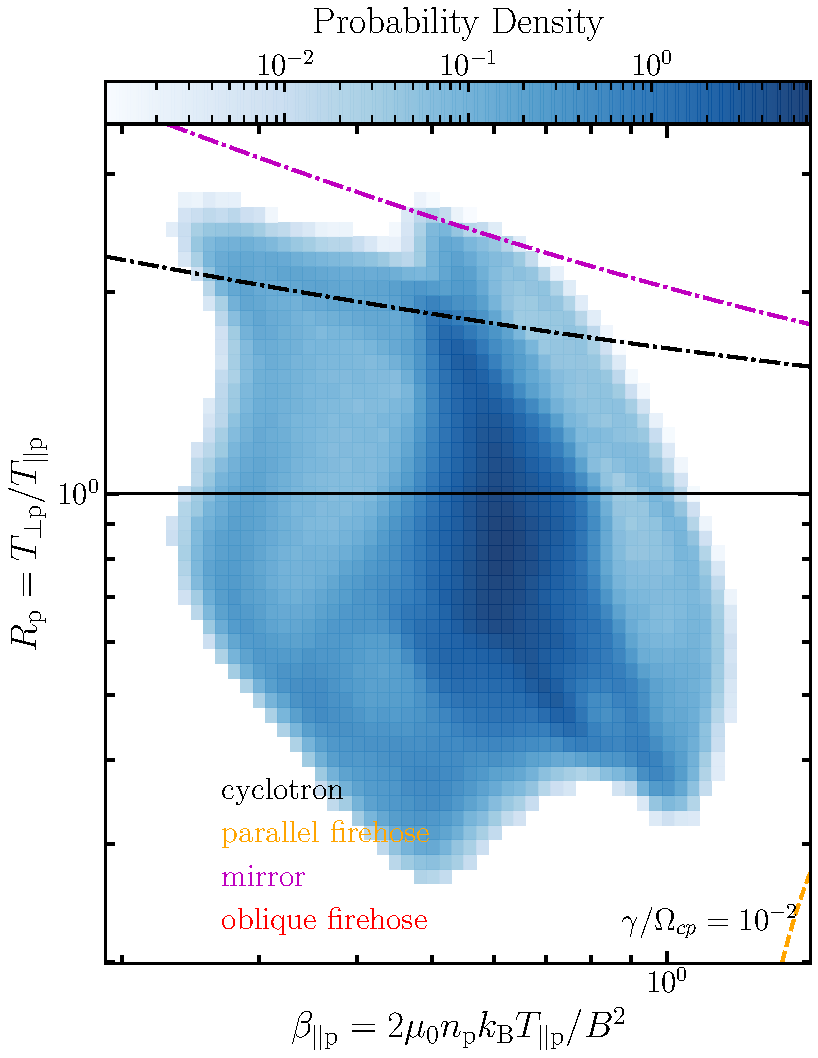
\includegraphics[width=1\textwidth]{figures/apdxA/brazil_prob_2dip.pdf}
            \caption[Brazil-plot of \texttt{149p6} dataset]{Plot of estimated probability density,
            $\Tilde{p}$ of ($R_{\rm p}, \beta_{\parallel \rm p}$) for \texttt{149p6} dataset and
            thresholds associated with different instabilities for threshold value of
            $\gamma_{\max}/\Omega_{\rm cp} = 10^{-3}$.}
            \label{fig:brazil_prob_2dip}
        \end{center}
    \end{figure}

    \begin{figure}
        \begin{center}
            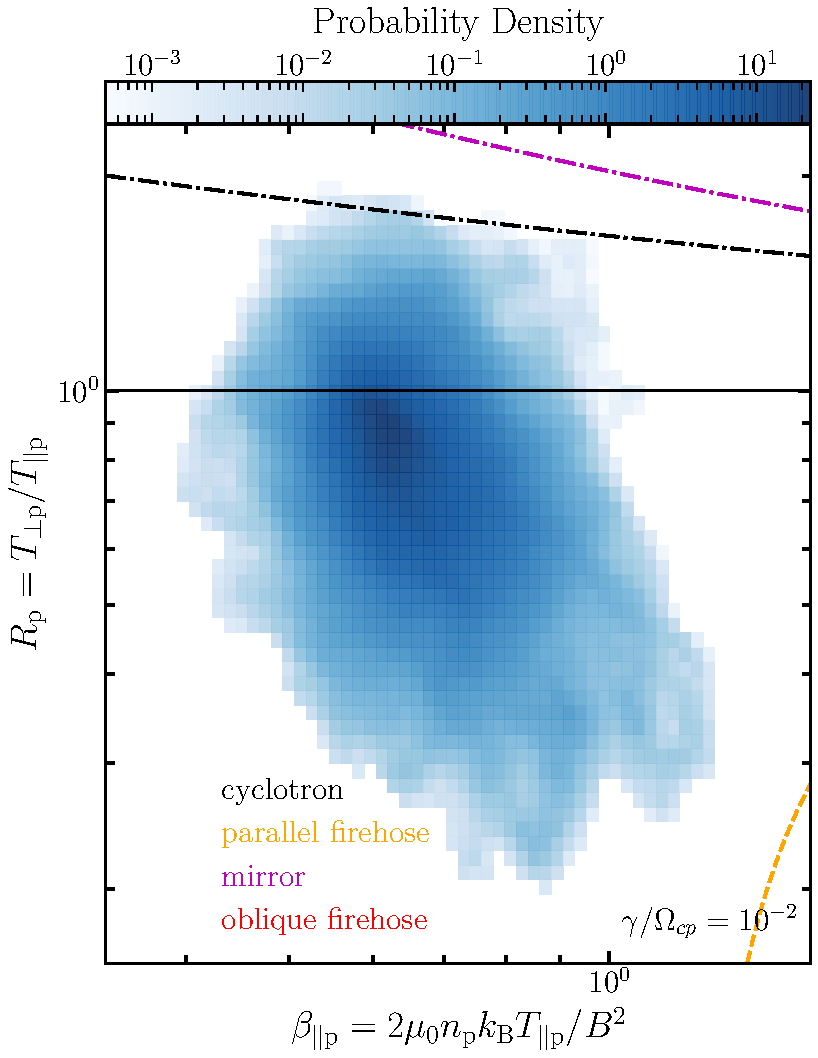
\includegraphics[width=1\textwidth]{figures/apdxA/brazil_prob_2dpp.pdf}
            \caption[Brazil-plot of \texttt{kaw} dataset]{Plot of estimated probability density,
            $\Tilde{p}$ of ($R_{\rm p}, \beta_{\parallel \rm p}$) for \texttt{kaw} dataset and
            thresholds associated with different instabilities for threshold value of
            $\gamma_{\max}/\Omega_{\rm cp} = 10^{-3}$.}
            \label{fig:brazil_prob_2dpp}
        \end{center}
    \end{figure}

    \begin{figure}
        \begin{center}
            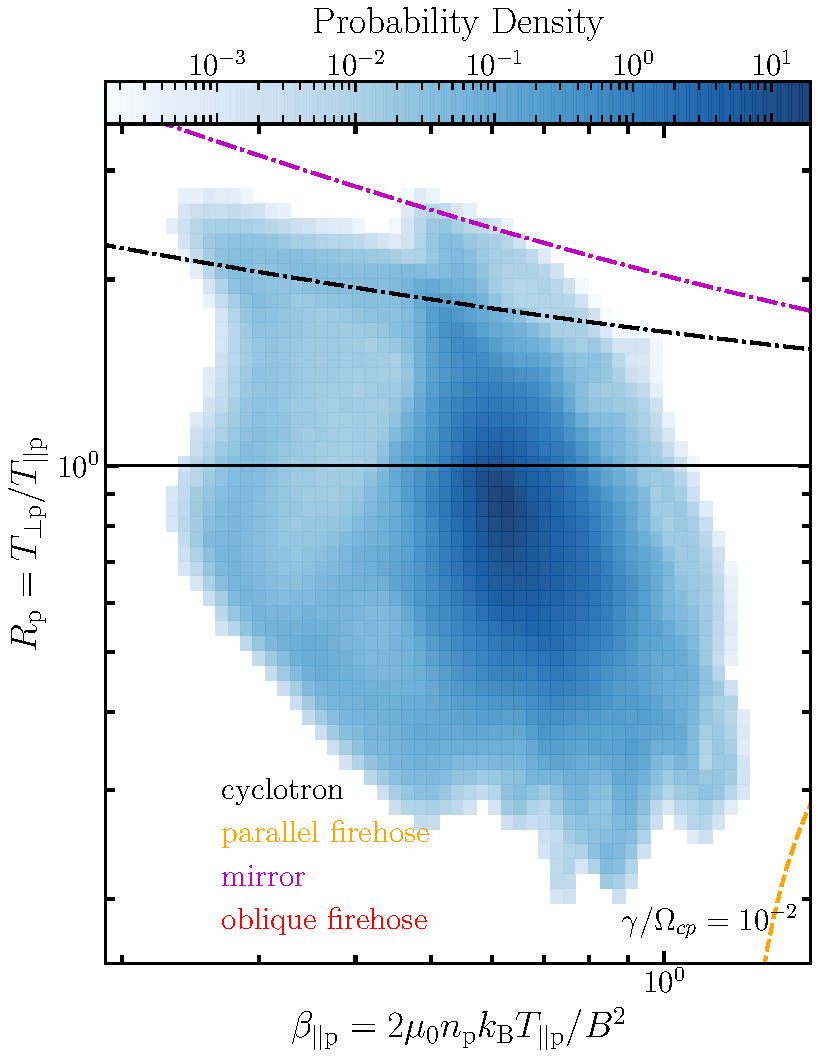
\includegraphics[width=1\textwidth]{figures/apdxA/brazil_prob_2d.pdf}
            \caption[Brazil-plot of \texttt{2dsim} dataset]{Plot of estimated probability density,
            $\Tilde{p}$ of ($R_{\rm p}, \beta_{\parallel \rm p}$) for combination of \texttt{149p6}
            and \texttt{kaw} dataset and thresholds associated with different instabilities for
            threshold value of $\gamma_{\max}/\Omega_{\rm cp} = 10^{-3}$.}
            \label{fig:brazil_prob_2d}
        \end{center}
    \end{figure}

    \begin{figure}
        \begin{center}
            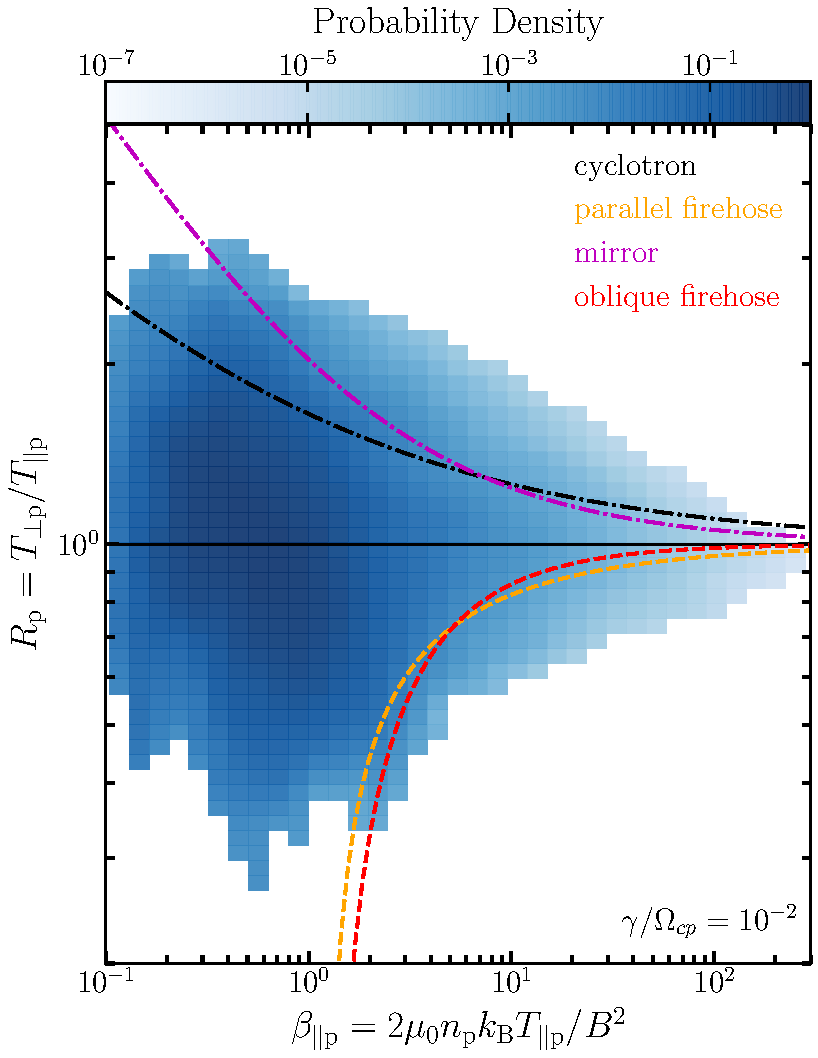
\includegraphics[width=1\textwidth]{figures/apdxA/brazil_prob_3d.pdf}
            \caption[Brazil-plot of \texttt{ros} dataset]{Plot of estimated probability density,
            $\Tilde{p}$ of ($R_{\rm p}, \beta_{\parallel \rm p}$) for \texttt{ros} dataset and
            thresholds associated with different instabilities for threshold value of
            $\gamma_{\max}/\Omega_{\rm cp} = 10^{-1}$.}
            \label{fig:brazil_prob_ros}
        \end{center}
    \end{figure}

    \begin{figure}
        \begin{center}
            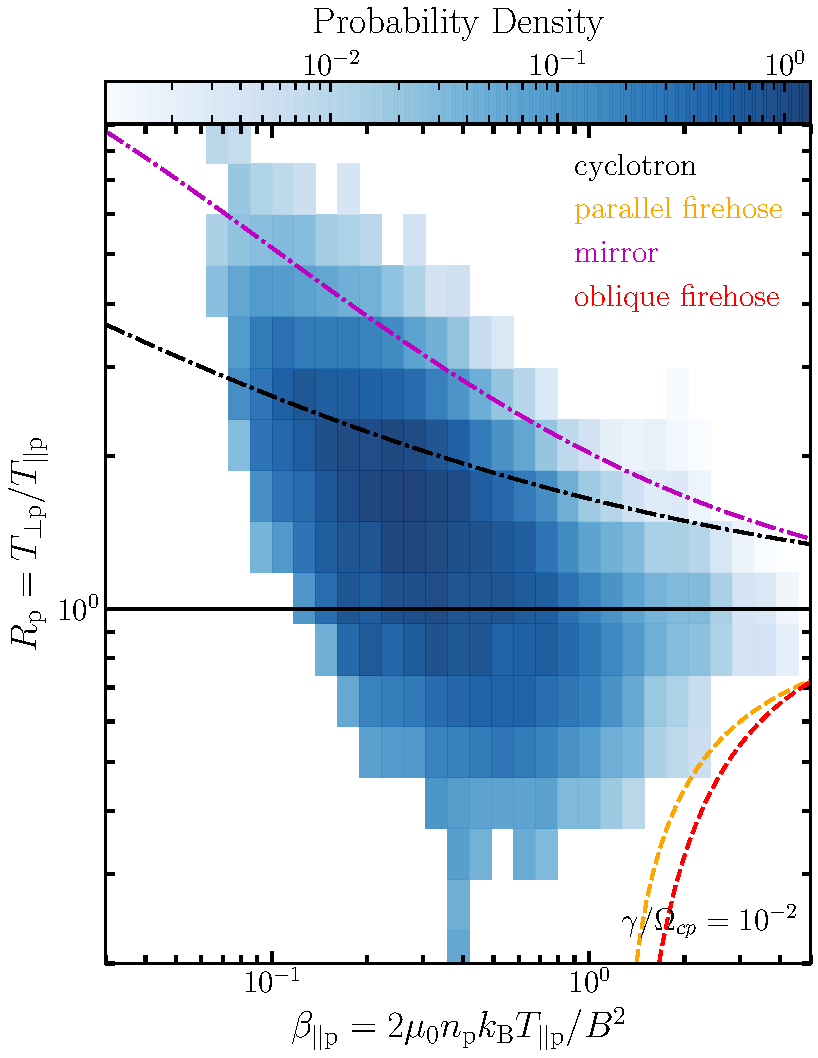
\includegraphics[width=1\textwidth]{figures/apdxA/brazil_prob_psp.pdf}
            \caption[Brazil-plot of \texttt{psp} dataset]{Plot of estimated probability density,
            $\Tilde{p}$ of ($R_{\rm p}, \beta_{\parallel \rm p}$) for \texttt{psp} dataset and
            thresholds associated with different instabilities for threshold value of
            $\gamma_{\max}/\Omega_{\rm cp} = 10^{-1}$.}
            \label{fig:brazil_prob_psp}
        \end{center}
    \end{figure}     % This file (appA.tex) contains the text
                   % for Appendix A. 

%
% This is the Appendix B file (appB.tex)
%
%\appendix{Equation of State} \label{apdx:B}
%
%    Equation 7.19 in \citet{Baumjohann1996} gives the relation between temperature and particle
%    density as:
%    \begin{align}
%        T ~\alpha~ n^{\gamma-1} \label{eq:adb1}
%    \end{align}
%    where $\gamma$ is the adiabatic index. And since particle flux density is conserved, assuming
%    constant velocity of particle, at any distance, $r$, from the Sun we have:
%    \begin{align}
%        n ~ 4\pi r^2 & = const.\\
%        \implies n ~ & \alpha ~ r^{-2} \label{eq:adb2}
%    \end{align}
%    Substituting for $r$ from \Cref{eq:adb2} in \Cref{eq:adb1} and using $\gamma = 5/3$, we have :
%    \begin{align}
%        T ~\alpha~ r^{-2(\gamma-1)}\\
%        \implies T ~\alpha~ r^{-4/3}
%    \end{align}

\appendix{CGL invariants} \label{apdx:B}

This appendix details the Chew–Goldberger–Low (CGL) invariants as mentioned in \Cref{sec:hop}.

%In a plasma for the $j^{\rm th}$ species, the \textit{energy density conservation equation} is
%given as: \begin{align} \frac{3}{2} n_{\rm j} k_{\rm B} \left( \frac{\partial T_{\rm j}}{\partial
%t} + \mathbf{v}_{\rm j} \cdot \nabla T_{\rm j} \right) + p_{\rm j} \nabla \cdot \mathbf{v}_{\rm j}
%= - \nabla \cdot \mathbf{q}_{\rm j} - \left(\mathbf{P}'_{\rm j} \cdot \nabla \right) \cdot
%\mathbf{v}_{\rm j} \label{eq:cgl1} \end{align} where $\mathbf{q}_{\rm j}$ is the heat flux vector,
%$\mathbf{P}_{\rm j}'$ is the stress tensor part of the full pressure tensor $\mathbf{P}_{\rm j}$
%and the other symbols have their usual meaning as define in the thesis.

%If we assume the pressure to be isotropic and that their time variations are happening
%adiabatically that is they are fast enough that no perceptible heat exchange takes place as the
%plasma evolves, then the right side of \Cref{eq:cgl1} is simply zero. And thus we can write the
%left side of the equation as: \begin{align} \frac{3}{2}\frac{d\left(n_{\rm j}\,k_{\rm B}\,T_{\rm
%j}\right)}{d\,t} - \frac{5}{2} k_{\rm B}\, T_{\rm j} \frac{dn_{\rm j}}{dt} & = 0 \label{eq:cgl2}
%\end{align} which is same as: \begin{align} n_{\rm j}\,\frac{dT_{\rm j}}{dt} - \frac{2}{3}\,T_{\rm
%j}\,\frac{dn_{\rm j}}{dt} & = 0 \label{eq:cgl3} \end{align}

As mentioned in \Cref{sec:hop}, for a slowly changing magnetic field (compared to the ion gyrotropic
time scale) we have conservation of magnetic moment ($\mu$) of the particle and thus we have:
\begin{align}
    \frac{d \mu}{dt} & = 0 \label{eq:cgl1}
\end{align}
where, $\mu = m_{\rm p}\,w_{\rm \perp p}^2/(2B)$, $m_{\rm p}$ is the proton mass, $w_{\rm \perp
p}^2$ is the perpendicular thermal velocity and $B$ is the magnitude of magnetic field. Writing
\Cref{eq:cgl1} in terms of proton-perpendicular temperature using \Cref{eq:temp}, we have:
\begin{align}
    \frac{d}{dt} \left(\frac{k_{\rm B} T_{\rm \perp p}}{B}\right) & = 0 \label{eq:cgl2}
\end{align}
or:
\begin{align}
    T_{\rm \perp p} & \propto B \label{eq:cgl3}
\end{align}

For the parallel case, consider the equation for parallel pressure ($p_\parallel$), for which under
similar assumptions one can write \citep{Baumjohann1996}:
\begin{align}
    p_\perp \, \frac{dp_\parallel}{dt} + 2\,p_\parallel\,\frac{dp_\perp}{dt} + 5\,p_\perp p_\parallel \, \nabla \cdot \mathbf{v} & = 0\label{eq:cgl4}
\end{align}
Substituting for $\nabla \cdot \mathbf{v}$ from the continuity equation (\Cref{eq:cgl5}),
\begin{align}
    \frac{\partial n}{\partial t} + \mathbf{v} \cdot \nabla n + n \nabla \cdot \mathbf{v} & = 0 \label{eq:cgl5}
\end{align}
and the fact that $d/dt = \partial/\partial t + \mathbf{v}\cdot\nabla$, we can rewrite
\Cref{eq:cgl4} as:
\begin{align}
    \frac{d}{dt}\left(\frac{p_\parallel p_\perp^2}{n^5} \right) & = 0 \label{eq:cgl6}
\end{align}
or:
\begin{align}
        \frac{d}{dt} \left(\frac{p_\parallel B^2}{n^3}\right) & = 0 \label{eq:cgl7}
\end{align}
which in terms of temperature can be written as:
\begin{align}
    T_\parallel \propto \left(n/B\right)^2 \label{eq:cgl8}
\end{align}
which is same as \Cref{eq:mu_4}.

\Cref{eq:cgl2,eq:cgl7} are referred as the \textit{Chew–Goldberger–Low} invariants.     % This file (appB.tex) contains the text
                   % for Appendix B.   

%
% This is the Appendix C file (appC.tex)
%
\appendix{Gaussian Processes Algorithm} \label{apdx:C}

    This appendix details the Gaussian Processes Regression followed in Section~\ref{sec:meth8}. We
    start with the \texttt{ros} dataset. As discussed in \Cref{sec:3pic} the dataset has a
    resolution of $2048^3$ cells with a box size of $\sim 42\,d_{\rm i}$. Since the resolution of
    reconstructed image is of the order of $d_{\rm i}$, we decided to downsample the dataset using
    \texttt{block\_reduce} in \texttt{skimage}. We lowered the resolution to 42 cells along $x$ and
    $y$-directions, and 128 cells along $z$-direction. In units of $d_{\rm i}$, this gives us
    resolution of $\sim 0.3\,d_{\rm i}$ in $z$-direction and $1\,d_{\rm i}$ along the other two. The
    reason for different resolutions is the fact that along $xy$-plane, the resolution is limited by
    the minimum separation between two spacecraft ($1\,d_{\rm i}$), whereas along the $z$-direction
    it is the sampling rate of our instrument which determines the resolution.
    
    Here we list typical values of some of the parameters associated with the simulation and solar
    wind at 1\,au:
    \begin{align*}
        d_i \rm{(1\,au)} & \sim 100 ~\rm{km} \\
        V_{sw} & \sim 500 ~\rm{km/sec} \\
        X_{sim} \rm{(box size)} & \sim 40\,d_{\rm i} \\
        & \sim 4\times 10^3\,\rm{km} \\
        d_{\rm spc} & \sim [1, 11]\,d_{\rm i} \\
        & \sim \rm{ [10^2, 10^3]\,km} \\
        f_{\rm min} & \sim V_{sw}/(2\times d_{spc, min}) \\
        & \sim 2.5\,\rm{Hz} \\
    \end{align*}
    At the assumed solar wind speed of $500\,\rm{km/s}$, it takes the spacecraft configuration
    roughly 10 seconds to cross the whole box. And because of Nyquist criteria, we must have a
    sampling rate faster than $2.5\,\rm{Hz}$. Because of restrictions provided by Nyquist frequency
    and the box size and because we wanted to have a sample at every plane along the $z$-direction,
    we chose a sampling frequency of $40\,\rm{Hz}$. This is easily achievable for modern day
    magnetometers \citep{Bale2016, Russell2016}.

    Once we have the sampling rate and the spacecraft configuration fixed, we virtually fly through
    the simulation box and collect data for each spacecraft. At the end of simulated flight we have
    $n_{\rm spc}$ (number of spacecraft) number of data points for each plane and thus $128 \times
    n_{\rm spc}$ total data points along with their positions. We then define a kernel and
    associated variables as: \\
    \texttt{pln} ~\texttt{=}~ \texttt{`xy'} \\
    \texttt{drn} ~\texttt{=}~ \texttt{`z'} \\
    \texttt{ck\_len} ~\texttt{=}~ \texttt{5} \\
    \texttt{mat\_len\_scl} ~\texttt{=}~ \texttt{[2,2,6]} \\
    \texttt{mat\_nu} ~\texttt{=}~ \texttt{5/2} \\
    \texttt{sigma\_0} ~\texttt{=}~ \texttt{0} \\
    \texttt{n\_restarts\_optimizer} ~\texttt{=}~ \texttt{20} \\
    \texttt{kernel} ~\texttt{=}~ \texttt{ CK(ck\_len, (1e-2, 1e2)) + CK(ck\_len, (1e-2, 1e2)) *} \\
    \indent \indent \texttt{Matern(length\_scale=mat\_len\_scl, nu=mat\_nu)} \\
    \\
    we then run the Gaussian Processes with the selected kernel:\\
    \texttt{gp} ~\texttt{=}~\texttt{GaussianProcessRegressor(kernel=kernel, } \\
    \indent \indent \texttt{n\_restarts\_optimizer=n\_restarts\_optimizer)} \\
    \\
    We can then get the model based on the data collected by the spacecraft:\\
    \texttt{gp.fit(X, y)} \\
    \\
    and then provide \texttt{gp.fit} with the coordinate of all the locations at which we want to
    find the value of the field:\\ 
    \texttt{y\_pred, mse\_pred = gp.predict(x1x2x3, return\_std=True)} \\
    \\
    and reshape the output get the final value of field at each point:\\
    \texttt{Zp = np.reshape(y\_pred,(indx\_max - indx\_min + 1,}\\
    \indent \texttt{indy\_max - indy\_min + 1, indz\_max - indz\_min + 1, 3))} \\
    \texttt{MSE = np.reshape(mse\_pred,(indx\_max - indx\_min + 1,} \\
    \indent \texttt{indy\_max - indy\_min + 1, indz\_max - indz\_min + 1))} \\
    %\end{flalign*}

    \texttt{Zp} is the output that we have plotted in \Crefrange{fig:gpr_cas_bx}{fig:gpr_bm}.     % This file (appC.tex) contains the text
                   % for Appendix C.

%
% This is the Appendix D file (appD.tex)
%
\appendix{Permission Letter} \label{apdx:D}

    Permission letter from the Physical Science Publication for
    \Cref{fig:brjhb,fig:spcsim,fig:pvi_hst_psp,fig:pvi_pdf_psp,fig:tem_pvi_lag}.
    \begin{figure*}[h!]
        \begin{center}
            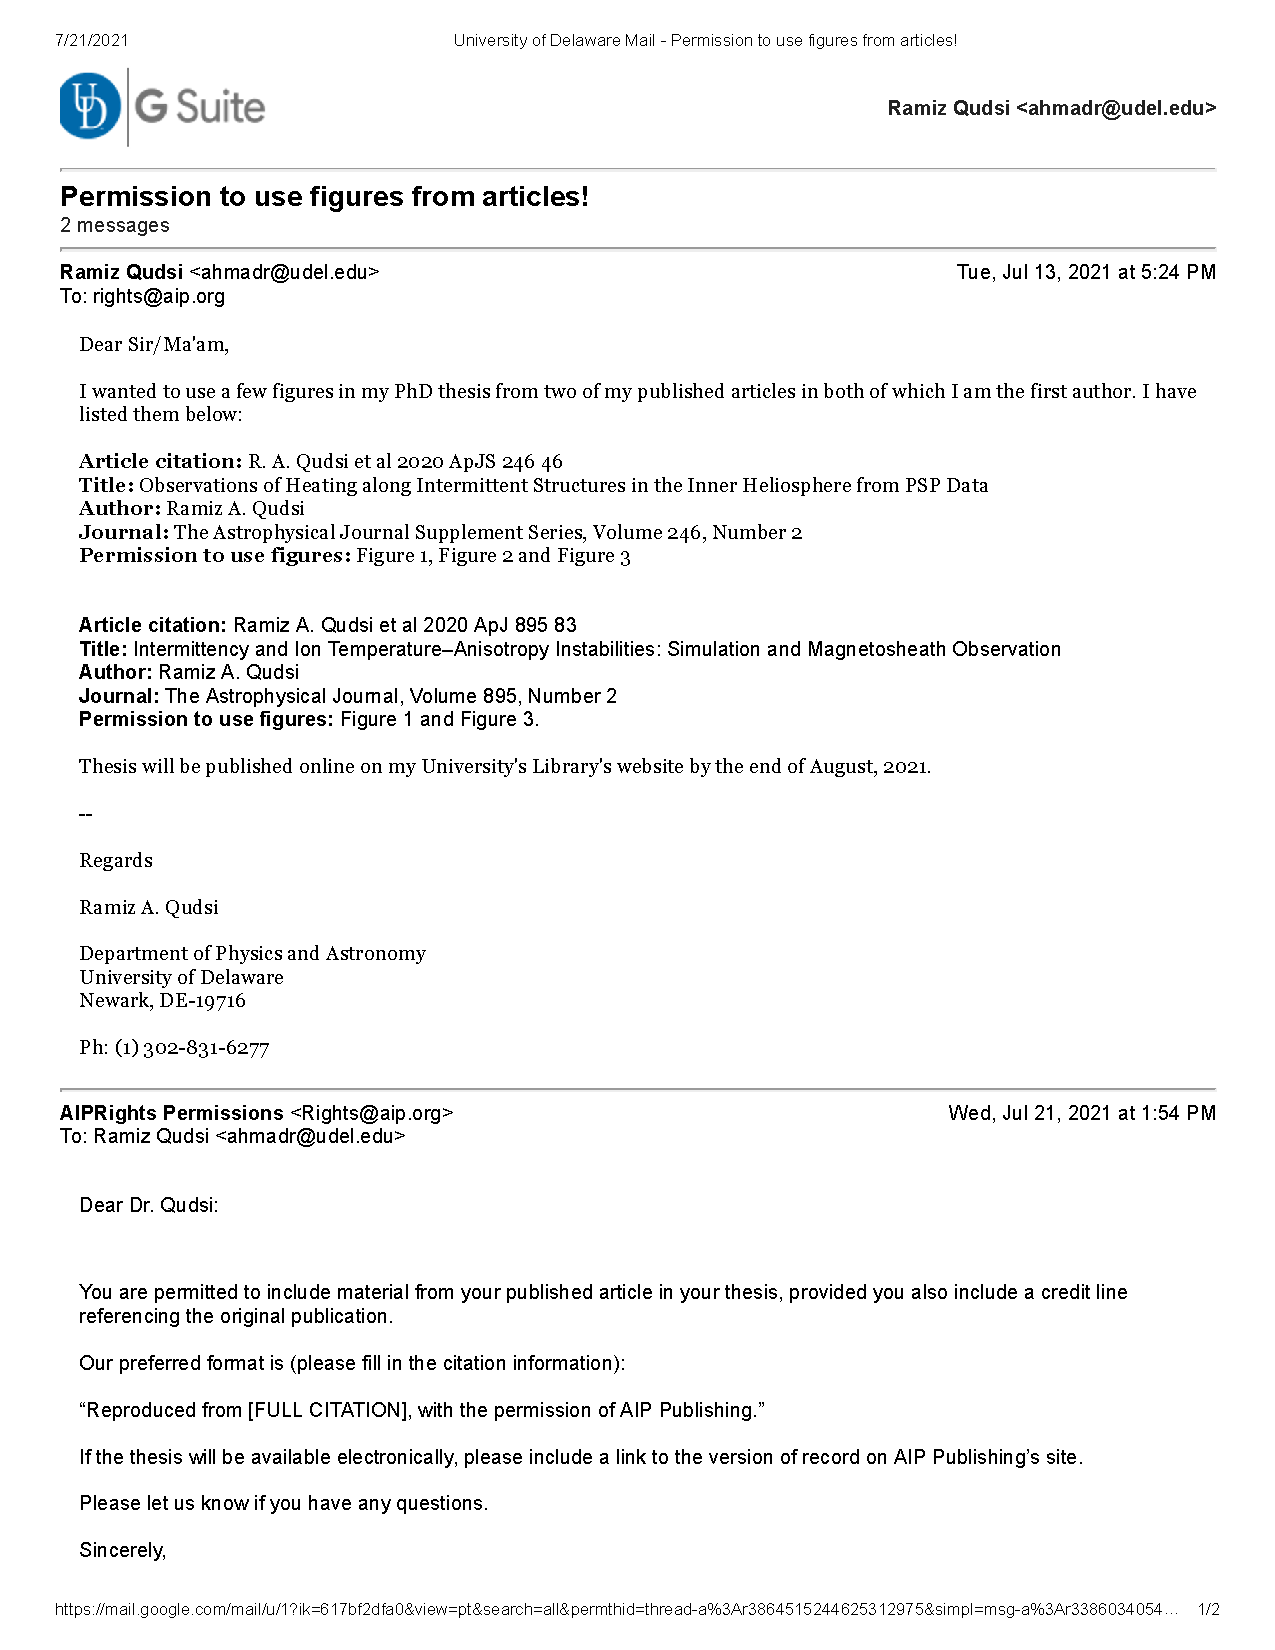
\includegraphics[width=0.7\textwidth]{figures/apdxD/apj_permission_letter.pdf}
            \captionsetup{labelformat=empty}
            \caption[]{}
            \label{fig:prmsn_ltr}
        \end{center}
    \end{figure*}     % This file (appD.tex) contains the text
                   % for Appendix D.

\printindex
\end{document}